\documentclass[12pt,english]{article}

%%%%%%%%%%%%%%%%%%%%%%%%%
%% SEC: PACKAGEs MAIN  %%
%%%%%%%%%%%%%%%%%%%%%%%%%
\usepackage{mathpazo}
\usepackage{eulervm}
\usepackage{amsmath}
\usepackage{amssymb}
\usepackage[utf8]{inputenc}
\usepackage[T1]{fontenc}
\usepackage{color}
% \usepackage[monochrome]{xcolor}
\usepackage{babel}
\usepackage{csquotes}
\usepackage{setspace}
\usepackage{graphicx}
\usepackage{booktabs,dcolumn}
\usepackage{array}
\usepackage{multirow}
\usepackage[font=singlespacing, skip=3pt]{caption}
\usepackage[usenames,dvipsnames,svgnames,table]{xcolor}
%\usepackage[usenames,dvipsnames,svgnames,table,monochrome]{xcolor} % test black and white color results, 2018-11-21 08:48
\usepackage{float}
\usepackage[export]{adjustbox}[2011/08/13]
\usepackage{enumitem}
% \usepackage{subfig}
%\usepackage[nolists, tablesfirst, nomarkers]{endfloat}
% \usepackage[unicode=true,pdfusetitle,
%  bookmarks=true,bookmarksnumbered=false,bookmarksopen=false,
%  breaklinks=false,pdfborder={0 0 1},backref=false,colorlinks=false]
%  {hyperref}
\usepackage[colorlinks=true, linkcolor=blue, citecolor=blue, plainpages=false, pdfpagelabels=true, urlcolor=blue]{hyperref}
\usepackage{geometry}
\usepackage{ragged2e}
\usepackage{appendix}
\usepackage{subcaption} % For subfigures

\usepackage{makecell}
\usepackage{adjustbox}
\usepackage{siunitx}
\usepackage{indentfirst}
\newcolumntype{d}{S[input-symbols = ()]}
\usepackage{lscape}
\usepackage{longtable}
\newcommand{\source}[1]{\caption*{Source: {#1}} }
\usepackage{threeparttable} % For tables with notes
\usepackage{threeparttablex} % For extending threeparttable functionality
\usepackage{pdflscape}

% Redefine the footnoterule command
\usepackage[hang,flushmargin]{footmisc}
\renewcommand{\footnoterule}{%
    \kern-3pt % Adjust the vertical position of the line
    \hrule width 0.2\columnwidth height 0.4pt % Width and height of the line
    \kern2.6pt % Adjust the spacing between the line and the footnotes
}

\renewcommand{\thetable}{\arabic{table}}
\renewcommand{\thefigure}{\arabic{figure}}

% *****************************************************************
% Estout LaTeX wrapper
% *****************************************************************

%%Original code developed by Jörg Weber: see
%% https://www.jwe.cc/2012/03/stata-latex-tables-estout/
%% andwho
%% https://www.jwe.cc/blog/


\let\estinput=\input % define a new input command so that we can still flatten the document

\newcommand{\estwide}[3]{
		\vspace{.75ex}{
			%\textsymbols% Note the added command here
			\begin{tabular*}
			{\textwidth}{@{\hskip\tabcolsep\extracolsep\fill}l*{#2}{#3}}
			\toprule
			\estinput{#1}
			\bottomrule
			\addlinespace[.75ex]
			\end{tabular*}
			}
		}	

\newcommand{\estauto}[3]{
		\vspace{.75ex}{
			%\textsymbols% Note the added command here
			\begin{tabular}{l*{#2}{#3}}
			\toprule
			\estinput{#1}
			\bottomrule
			\addlinespace[.75ex]
			\end{tabular}
			}
		}

% Allow line breaks with \ in specialcells
\newcommand{\specialcell}[2][c]{%
    \begin{tabular}[#1]{@{}c@{}}#2\end{tabular}
}

% \newcommand{\sym}[1]{\rlap{#1}}% Thanks David Carlisle


%%%%%%%%%%% End of wrapper %%%%%%%%%%%%%%%%%%%%%
    
%%%%%%%%%%% TiKz %%%%%%%%%%%%%%%%%%%%%
\usepackage{tikz}
\usetikzlibrary{shapes.geometric, arrows}

\tikzstyle{startstop} = [rectangle, rounded corners, minimum width=3cm, minimum height=1cm,text centered, draw=black, fill=red!30]

\tikzstyle{io} = [trapezium, trapezium left angle=70, trapezium right angle=110, minimum width=3cm, minimum height=1cm, text centered, text width =5cm, draw=black, fill=blue!30]

\tikzstyle{process} = [rectangle, minimum width=3cm, minimum height=1cm, text centered, text width =5cm, draw=black, fill=orange!30]

\tikzstyle{decision} = [diamond, minimum width=3cm, minimum height=1cm, text centered, draw=black, fill=green!30]

\tikzstyle{arrow} = [thick,->,>=stealth]

% Citation comes loading other packages, so that footnotes follow biblatex-chicago style
%%%%%%%%%%%%%%%%%%%%%%%%
%% SEC: Bibliography %%
%%%%%%%%%%%%%%%%%%%%%%%%
\usepackage[authordate,
backend=bibtex,
doi=false,
isbn=false,
sorting=nyt,
maxbibnames=10,
maxcitenames=3,
sortcites=False]{biblatex-chicago}


% \bibliography{../_bib/ref_one, ../_bib/ref_two, ../_bib/ref_three, ../_bib/ref_four, ../_bib/ref_five}

\AtEveryBibitem{\clearlist{note}\clearlist{language}\clearlist{issn}} % clears issn
\AtEveryBibitem{%
	\ifentrytype{online}{%
		\clearfield{urlyear}
		\clearfield{urlmonth}
		\clearfield{urlday}
		\clearfield{note}
		\clearlist{language}
	}{%
		\clearfield{eprint}%
		\clearfield{url}%
		\clearfield{urlyear}
		\clearfield{urlmonth}
		\clearfield{urlday}
		\clearfield{note}
		\clearlist{language}
	}
}

% \renewcommand*{\bibfont}{\small}


% Responses to Referees
\usepackage{blindtext}
\newcommand{\aptxspc}{1.8}
\newcommand{\rrquote}{1.1}
\newcommand{\rrxspc}{1.5}

\begin{document}

% SUBMISSION COVER
\thispagestyle{empty}
\begingroup
  \doublespacing
  \centering
  \LARGE REVISE \& RESUBMIT SUBMISSION\\[0.25em]
  \LARGE Journal of Policy Analysis and Management \\[0.25em]
  \LARGE MANUSCRIPT ID: JPAM-2025-13688 \\[1.0em]
\endgroup
This document and the associated contents in the accepted version of JPAM-2025-13688 for the Journal of Policy Analysis and Management. I include:
\begin{enumerate}
    \item Title page information
    \begin{itemize}
        \item Title and Author
        \item Abstract
        \item Keywords
        \item Acknowledgment
    \end{itemize}
    \item The manuscript
    \begin{itemize}
        \item Main manuscript text
        \item Main manuscript references
        \item Main manuscript figures
        \item Main manuscript tables
    \end{itemize}  
    \item \hyperref[r&r:responses]{Responses to the editor and referees comments}
    \item The online appendix, which is separately paged. It includes an online appendix title page, appendix A, appendix B, appendix C, and references for citations in the appendix.
\end{enumerate}
\clearpage


%%%%%%%%%%%%%%%%%%%%%%%%%%%%%%%%%%%%%%%%
% Part I. Title Page, Authors, Abstract, etc. 
%%%%%%%%%%%%%%%%%%%%%%%%%%%%%%%%%%%%%%%%
% Load in title page information, title, author information, abstract, etc are stored here

%%%%%%%%%%%%%%%%%%%%%%%%%%%%%%%%%%%%%%%%
% 1. Define Keywords, JEL
%%%%%%%%%%%%%%%%%%%%%%%%%%%%%%%%%%%%%%%%
\newcommand{\PAPERKEYWORDS}{\textbf{Keywords}: Economics of Minorities, Race, and Immigrants; Discrimination and Prejudice; Stratification Economics}
\newcommand{\PAPERJEL}{\textbf{JEL}: I310, J15, J71, Z13}

%%%%%%%%%%%%%%%%%%%%%%%%%%%%%%%%%%%%%%%%
% 2. Define Title
%%%%%%%%%%%%%%%%%%%%%%%%%%%%%%%%%%%%%%%%
\newcommand{\PAPERTITLE}{The Effect of Racial and Ethnic Attitudes on Asian Identity in the U.S}

%%%%%%%%%%%%%%%%%%%%%%%%%%%%%%%%%%%%%%%%
% 3. Define Authors contact information
%%%%%%%%%%%%%%%%%%%%%%%%%%%%%%%%%%%%%%%%
\newcommand{\AUTHORHADAH}{Hussain Hadah}
\newcommand{\AUTHORHADAHURL}{https://orcid.org/0000-0002-8705-6386}
\newcommand{\AUTHORHADAHINFO}{\href{\AUTHORHADAHURL}{\AUTHORHADAH}: The Murphy Institute and Department of Economics, Tulane University, Caroline Richardson Building, 62 Newcomb Place, Suite 118, New Orleans, LA 70118, United States (e-mail: \href{mailto:hhadah@tulane.edu}{hhadah@tulane.edu}, phone: +1-602-393-8077)}


%%%%%%%%%%%%%%%%%%%%%%%%%%%%%%%%%%%%%%%%
% 4. Define Thanks
%%%%%%%%%%%%%%%%%%%%%%%%%%%%%%%%%%%%%%%%
\newcommand{\ACKNOWLEDGMENTS}{
 I thank Patrick Button, Willa Friedman, Chinhui Juhn, Vikram Maheshri, and Yona Rubinstein for their support and advice. I also thank Aimee Chin, Steven Craig, German Cubas, Elaine Liu, Fan Wang, and the participants of the Applied Microeconomics Workshop at the University of Houston, the European Society for Population Economics (ESPE), the anonymous referees, and the editor for their helpful feedback.}

%%%%%%%%%%%%%%%%%%%%%%%%%%%%%%%%%%%%%%%%
% 5. Define Abstract
%%%%%%%%%%%%%%%%%%%%%%%%%%%%%%%%%%%%%%%%
\newcommand{\PAPERABSTRACT}{
I study the determinants of the choice to identify as Asian among those who could—those whose parents, grandparents, or selves were born in an Asian country. Using a multiple proxy regression approach, I construct a bias measure based on the Implicit Association Test (IAT), the American National Election Studies (ANES), and hate crimes against Asians. I find that individuals with Asian ancestry are significantly less likely to self-identify as Asian if they live in states with high levels of bias. A one standard deviation increase in bias decreases self-reported Asian identity by 9 percentage points across all generations. The effects vary by generation and family type: bias decreases Asian racial identity by 5 percentage points among first-generation immigrants (statistically insignificant), 8 percentage points among second-generation, and 8 percentage points among third-generation Asian Americans. Mixed-race families show the strongest responses, with bias decreasing Asian racial identity by 15 percentage points among children of Asian fathers and White mothers, and 10 percentage points among children of White fathers and Asian mothers. Using multinomial logit regression, I find that high bias environments drive substantial shifts from ``Asian only'' to ``White only'' racial identity, with probabilities changing by up to 50 percentage points. Higher parental education and income generally increase the probability of reporting Asian identity, with particularly strong effects among mixed-race children. These findings have implications for the interpretation of research on racial and ethnic gaps in economic outcomes and accurate population measurement. \PAPERJEL}

%%%%%%%%%%%%%%%%%%%%%%%%%%%%%%%%%%%%%%%%
% 6. Define citation or availability of latest draft
%%%%%%%%%%%%%%%%%%%%%%%%%%%%%%%%%%%%%%%%
\newcommand{\PAPERDOIURL}{https://doi.org/10.1086/711654}
\newcommand{\PAPERINFO}{

 \url{\PAPERDOIURL}.
}
\pagenumbering{roman}
\setcounter{page}{1}

% Part I.a.1 Title
\section*{TITLE AND AUTHORS}
\subsection*{TITLE AND RUNNING HEAD}
\begin{itemize}[label={}, leftmargin=*]
    \item Title: \textbf{\PAPERTITLE}
    \item Running Head:  \textbf{Bias and Asian Identity}
\end{itemize}
% Part I.a.2 Author info
\subsection*{AUTHORS}
\begin{itemize}[label={}, leftmargin=*]
    \item List of authors:
    \begin{enumerate}
        \item \AUTHORHADAHINFO
    \end{enumerate}
    \item Corresponding author:
    \begin{itemize}
        \item \textbf{\AUTHORHADAHINFO}
    \end{itemize}
\end{itemize}

\subsection*{Data Availability Statement}
The data that support the findings of this study will be openly available to all researchers after the review process. For immediate information regarding the data and/or computer programs used for this study, please contact Hussain Hadah at hhadah@tulane.edu.

\subsection*{Funding Statement}

The author has no funding for the research, authorship, and/or publication of this article to report.

\subsection*{Conflict of Interest Disclosure}
The author declare that they have no conflicts of interest regarding the publication of this manuscript.

\clearpage 

% Part I.b Abstract
\doublespacing
\section*{ABSTRACT}
% \begin{myRaggedRight}
\PAPERABSTRACT
% \end{myRaggedRight}
\clearpage 

% Part I.c Keywords
\doublespacing
\section*{KEYWORDS}
\PAPERKEYWORDS
\clearpage 

% Part IV.d Acknowledgements
\doublespacing
\section*{ACKNOWLEDGMENT}
% \begin{myRaggedRight}
\ACKNOWLEDGMENTS
% \end{myRaggedRight}
\clearpage 

%%%%%%%%%%%%%%%%%%%%%%%%%%%%%%%%%%%%
% Part II. Manuscript main text
%%%%%%%%%%%%%%%%%%%%%%%%%%%%%%%%%%%%
\pagenumbering{arabic}
\setcounter{page}{1}
\renewcommand*{\thefootnote}{\arabic{footnote}}
\begingroup
  \centering
  \Large MANUSCRIPT TEXT\\[1em]
\endgroup
% Manuscript main text
% \begin{myRaggedRight}
%%%%%%%%%%%%%%%%%%%%%%%%%%%%%%%%%%%
% Main Text
%%%%%%%%%%%%%%%%%%%%%%%%%%%%%%%%%%%

\section{Introduction}\label{sec:intro}

Asian Americans represent the fastest-growing racial group in the United States, yet their experiences with discrimination and identity formation remain underexplored in economic research.\footnote{The 2020 Census counted more than 20 million Asian Americans---6.4 percent of the population---nearly double the number counted two decades earlier \autocite{floodsarahIntegratedPublicUse2021a}. The Asian American population numbers are based on the author's calculations from the Current Population Survey and US Census data.} Unlike other minority groups, Asian Americans occupy a distinctive position in America's racial hierarchy—simultaneously experiencing discrimination while being characterized through the ``model minority'' stereotype. This dual status creates complex incentives around racial identity choices that fundamentally differ from other groups' experiences, as Asian identification can signal both academic excellence and perpetual foreignness.

An extensive literature has documented Asian-White gaps in various outcomes \autocite{chiswick1983analysis, duleep2012economic, hilger2016upward, arabsheibani2010asian}, yet the role of identity selection in shaping these disparities remains understudied. The challenge lies in defining and measuring racial identity, particularly when individuals possess agency in how they racially self-identify. To the extent that reporting Asian racial identity represents a strategic choice influenced by local discrimination, measured gaps may systematically vary across geographic contexts in ways that previous research has not fully explored.

Various contextual factors, including anti-Asian sentiment and stereotype threat, can influence how individuals navigate their racial identity choices. Recent events have brought renewed attention to how external hostility shapes Asian American experiences. In this paper, I examine the determinants of Asian racial identity reporting and analyze how Asian Americans strategically select between Asian and White racial identities. Specifically, I investigate how anti-Asian bias shapes decisions to racially identify, or not, as Asian American.

This paper has important implications for several reasons. First, if individuals respond to prejudice by avoiding Asian racial identification, conventional analyses of racial gaps may systematically overestimate disparities in the most prejudiced areas. This would lead to misunderstanding of both the extent and geographic distribution of discrimination against Asian Americans. Second, identity choices may influence measured labor market trajectories among racial groups, potentially making Asian American integration appear more successful than reality suggests, thereby reinforcing model minority stereotypes that obscure genuine barriers faced by Asian American communities. Third, strategic identity reporting affects the enumeration of Asian American populations, with implications for political representation, resource allocation, and the design of policies aimed at addressing racial inequities.

I explore how individual characteristics and societal attitudes toward Asian Americans influence racial identity reporting. I utilize identity and ancestry data from the Current Population Survey (CPS) combined with measures of anti-Asian bias derived from Harvard's Project Implicit Association Test (IAT), the American National Election Studies (ANES), and hate crimes targeting Asian Americans.\footnote{The IAT data comes from Harvard's Project Implicit \autocite{greenwaldMeasuringIndividualDifferences1998}. Implicit bias measures have gained prominence in economics, with IAT scores correlating with economic outcomes \autocite{chettyRaceEconomicOpportunity2020,gloverDiscriminationSelfFulfillingProphecy2017}, voting patterns \autocite{friesePredictingVotingBehavior2007}, and health disparities \autocite{leitnerRacialBiasAssociated2016}.} I ground my analysis in a theoretical framework of \textcite{akerlofEconomicsIdentity2000}, explicitly modeling how external prejudice creates differential utility from identity choices and establishing conditions under which individuals strategically modify their racial self-presentation.

Measuring identity choices outside of lab settings presents is challenging, requiring both objective ancestry indicators and subjective identity measures. I leverage birthplace and ancestry data to construct objective Asian ancestry measures, then analyze deviations between objective ancestry and subjective racial identification. The analysis reveals that racial identity reporting negatively correlates with individual characteristics like parental education, and with environmental factors reflecting local discrimination levels.

Among individuals with Asian ancestry, I document that heightened anti-Asian bias correlates with reduced Asian racial identity reporting. Specifically, a one standard deviation increase in bias corresponds to a statistically significant 9 percentage point decrease in Asian racial identification among first-generation immigrants, a statistically insignificant 5 percentage point decrease among second-generation individuals, and a statistically significant 8 percentage point decrease among third-generation Asian Americans. The analysis by family structure reveals additional heterogeneity: bias effects prove strongest among children from mixed-race families, with a one standard deviation bias increase correlating with a 15 percentage point decrease in Asian identification among children of Asian fathers and White mothers, and a 10 percentage point decrease among children of White fathers and Asian mothers. These patterns suggest that economically successful Asian Americans—those with higher education and wealth—may strategically avoid Asian racial identification, leading research using subjective measures to underestimate Asian-White gaps in highly prejudiced areas.

This research contributes to multiple scholarly literatures in economics. First, it extends the economics of identity framework by examining how racial stereotypes—both positive and negative—influence identity choices \autocite{akerlofEconomicsIdentity2000}. Building on \textcite{charnessSocialIdentityGroup2020} and \textcite{atkinHowWeChoose2021}, I show that Asian Americans face a complex utility landscape where Asian identity can simultaneously signal competence (in educational contexts) and foreignness (in social settings).

The analysis connects to stratification economics research examining how racial hierarchies shape economic outcomes \autocite{darityEconomicsIdentityOrigin2006,darityPositionPossessionsStratification2022}. This framework extends to Asian American experiences, where model minority stereotypes create unique forms of racialization distinct from other groups' experiences \autocite{goldsmithDarkLightSkin2007,hamiltonSheddingLightMarriage2009,dietteSkinShadeStratification2015}.

While my formal theoretical model provides a logical framework for understanding how bias affects racial identity, the behavioral literature on racial identity and assimilation offers crucial empirical insights that complement this theoretical approach. Research in this tradition emphasizes how racial identity is not merely a cognitive construct but is actively performed, negotiated, and reconstructed through daily interactions and life experiences \autocite{waters1990ethnic}. \textcite{telles2008generations} study of Mexican Americans demonstrates how individuals strategically adapting their racial presentations across different social contexts while maintaining core identity elements across generations. Similarly, behavioral studies have documented how discrimination experiences shape identity salience and group attachment, with individuals developing adaptive strategies that range from ethnic distancing to reactive ethnicity depending on situational factors \autocite{zhou1997segmented}. This behavioral perspective reveals that racial identity operates as both a response to external categorization and an active process of boundary maintenance \autocite{cornell2006ethnicity}. While this literature has primarily relied on qualitative observations and ethnographic methods to document identity flexibility, the present analysis advances this understanding by quantifying these strategic choices through systematic comparison of objective ancestry measures with subjective racial identification across varying environmental contexts.

The paper also contributes to research on discrimination in economic contexts. \textcite{bertrandAreEmilyGreg2004} and \textcite{charlesPrejudiceWagesEmpirical2008} demonstrate how prejudice affects labor market outcomes, while recent work by \textcite{bursztynImmigrantNextDoor2022} explores how long-term exposure shapes attitudes. My analysis extends this literature by examining how discrimination influences the fundamental question of racial self-identification.

Within immigration and integration research, this work builds on studies examining how Asian Americans navigate assimilation processes \autocite{abramitzkyCulturalAssimilationAge2016,abramitzkyNationImmigrantsAssimilation2014}. Unlike European immigrant groups, Asian Americans face persistent ``perpetual foreigner'' stereotypes that complicate integration patterns regardless of generational status \autocite{foukaImmigrantsAmericansRace2022}. The model minority myth creates additional complexity, as Asian identification may carry both benefits and costs depending on context \autocite{mengIntermarriageEconomicAssimilation2005}.

This paper most closely relates to recent economic research on racial identity fluidity and strategic ethnic identification \autocite{hadah2024hispanicidentity, antmanEthnicAttritionObserved2016,antmanIncentivesIdentifyRacial2015,antmanAmericanIndianCasinos2021}. However, while previous work focused primarily on Hispanic ethnic attrition, Asian American identity choices operate through different economic mechanisms due to distinct stereotypes, discrimination patterns, and socioeconomic profiles. The concept of ``racial identity flexibility'' among Asian Americans reflects both the economic advantages and constraints of model minority positioning.

Recent work in behavioral economics provides additional context for understanding these identity choices. \textcite{bordaloStereotypes2016} demonstrate how stereotypes influence economic decision-making, while \textcite{bonomiIdentityBeliefsPolitical2021} show how identity affects political and economic preferences. My analysis contributes to this literature by showing how external discrimination shapes the fundamental choice of racial identity.

Taking into consideration the identity flexibility that characterizes Asian American experiences, I investigate the economic determinants driving racial self-identification decisions. \textcite{hadah2024hispanicidentity} finds that bias and self-reported Hispanic identity are negatively associated among objectively Hispanic immigrants. I aim to examine how certain personal and environmental factors influence the complexity of endogenous racial identity among Asian Americans, recognizing that the model minority stereotype creates unique economic incentive structures not present for other groups.

The empirical analysis documents how observable characteristics—individual traits and societal attitudes—affect racial identity reporting among Asian Americans. These findings have important implications for measuring racial economic disparities and understanding how discrimination operates in modern labor markets.

\section{Theoretical Framework}\label{sec:model}

I develop a theoretical framework for understanding racial identity choice that extends \textcite{akerlofEconomicsIdentity2000} to incorporate stereotype-specific costs and benefits. Unlike generic minority identification models, this framework recognizes that Asian Americans face unique utility trade-offs where racial identity can signal both positive attributes (academic achievement, work ethic) and negative characteristics (foreignness, social exclusion).

Formally, individual $i$ belongs to racial group $r_i \in \{A, W\}$, where $A$ represents Asian and $W$ represents White. Agent $i$'s utility depends on their actions and how those actions interact with their chosen racial identity $I_i$:

\begin{equation}
U_i = U_i(\pmb{a_i}, \pmb{a_{-i}}, I_i)\label{eq:util}
\end{equation}

Individual identity $I_i$ reflects personal actions, others' behaviors toward them, and societal expectations associated with their racial group:

\begin{equation}
I_i = I_i(\pmb{a_i}, \pmb{a_{-i}}; \pmb{S}_{r_{i}})\label{eq:identity}
\end{equation}

Where $\pmb{a_i}$ represents individual $i$'s actions, $\pmb{a_{-i}}$ captures others' actions affecting $i$'s identity (including anti-Asian bias), and $\pmb{S}_{r_{i}}$ denotes societal stereotypes and expectations associated with racial group membership.\footnote{This extends \textcite{akerlofEconomicsIdentity2000}'s proscription concept to encompass both negative stereotypes and positive model minority expectations.}

The key insight for Asian Americans is that $\pmb{S}_{A}$ includes both positive stereotypes (academic excellence, economic success) and negative ones (perpetual foreigner status, social exclusion). This creates context-dependent utility from Asian identification—beneficial in some settings (academic achievement contexts) but costly in others (social acceptance, political inclusion).

Individual $i$ selects actions $a_i$ to maximize utility given their racial group $r_i$, associated stereotypes $\pmb{S}_{r_{i}}$, and others' actions $\pmb{a_{-i}}$. The first-order condition becomes:

\begin{equation}
\frac{\partial U_i}{\partial a_i} + \frac{\partial U_i}{\partial I_i} \cdot \frac{d I_i}{d a_i} = 0\label{eq:foc}
\end{equation}

The solution $a_{i}^{\star}$ yields utility $U_{i}^{\star}$. Now suppose individuals can strategically choose their racial identity at cost $c$. They will switch identities when $\tilde{U_{i}}^{\star} \geq U_{i}^{\star} + c$, where $\tilde{U_{i}}^{\star}$ represents utility under the alternative racial identity.

Identity switching occurs when benefits $\tilde{U_{i}}^{\star} - U_{i}^{\star}$ exceed costs $c$. These net benefits are non-zero only when $\frac{d I_i}{d a_i} \neq 0$ and $\frac{\partial U_i}{\partial I_i} \neq 0$. This framework suggests empirical analysis should focus on: (1) individual characteristics affecting optimal actions under different racial identities, (2) contextual factors (anti-Asian bias) creating differential treatment by racial group, (3) populations with low switching costs $c$, and (4) groups whose utility significantly depends on racial identity.

From the empirical analysis, I investigate characteristics affecting individual actions under different identity choices from point (1). These characteristics include immigrant generation, mixed-race versus mono-racial family structure, etc. I also examine how anti-Asian bias influences identity choices. Finally, restricting analysis to individuals with low identity switching costs $c$ ensures the sample excludes populations unlikely to modify racial identification—for example, non-Asian Whites without Asian ancestry.

The model predicts that anti-Asian bias increases the utility differential between White and Asian identification, making identity switching more attractive. Mixed-race individuals face lower switching costs due to phenotypic ambiguity, while later-generation Asian Americans may find identity switching more feasible due to cultural assimilation.

\section{Data Sources and Measurement Strategy}\label{sec:data}

This section describes the datasets employed in the analysis. To examine relationships between social attitudes and Asian racial identity reporting, I require both subjective and objective Asian identity measures for selecting appropriate Asian American subgroups. I utilize the Integrated Public Use Microdata Series (IPUMS) Current Population Survey (CPS) \autocite{floodsarahIntegratedPublicUse2021a} with ancestry information to construct objective identity measures. I develop composite anti-Asian bias measures using \textcite{lubotskyInterpretationRegressionsMultiple2006}'s methodology to reduce attenuation bias.

\subsection{Measuring Asian Racial Identity}\label{subsec:cps}

I measure Asian racial identity using Current Population Survey (CPS) data from 2004-2021, enabling construction of objective Asian ancestry measures for minors living with parents. Following \textcite{antmanEthnicAttritionObserved2016,antmanEthnicAttritionAssimilation2020}, I utilize birthplace information for individuals, parents, and grandparents to create objective Asian ancestry indicators.\footnote{This approach parallels previous research but focuses on racial rather than ethnic categorization.} The methodology allows perfect identification of first-, second-, and third-generation Asian Americans (see Figure \ref{fig:diag} for visual representation). This approach enables construction of objective Asian ancestry measures for minors under age 17 living with parents. I also use another CPS sample of adults aged 18+ to examine whether their racial identity reporting patterns differ from minors. For the adult sample, I can only identify first- and second-generation.\footnote{Since adults still living with parents are might not representative of the overall adult population and is a rare occurrence, I do not link adults to their parents.}

The objective ancestry measure—distinct from subjective racial identification where respondents select ``Asian'' as their race—depends on birthplaces across three generations.\footnote{For this analysis, Asian countries comprise East Asian and Southeast Asian nations, including China, Hong Kong, Taiwan, Japan, Korea, Mongolia, Cambodia, Indonesia, Laos, Malaysia, Philippines, Singapore, Thailand, and Vietnam, but exclude South Asian and Middle Eastern countries, consistent with standard demographic classifications.} The three identifiable generations include: 1) first-generation immigrants born in Asian countries with both parents also born in Asian countries, 2) second-generation individuals who are US-born citizens with at least one parent born in an Asian country, 3) third-generation Asian Americans who are US-born citizens with two US-born parents and at least one grandparent born in an Asian country. It is important to note that while the ancestry measure provides an objective assessment of Asian heritage, it may not capture all nuances of racial identity. For instance, White individuals with Asian ancestry born to non-Asian parents in Asia, such as on American military bases, may not be classified as Asian in the data. To avoid potential misclassification, I remove individuals who report that they were born abroad of American parents. The sample includes Asian Americans, first-, second-, and third-generation immigrants aged 17 and younger living with parents between 2004 and 2021. Summary statistics appear in Table (\ref{tab:sumstat1}). The adult sample includes first- and second-generation Asian American immigrants aged 18 and older between 2004 and 2021. The summary statistics for the adult sample appear in Table (\ref{tab:sumstat-adults}). 

While CPS relies on household respondents (parents or caregivers) to report children's racial identity, this proxy reporting likely reflects children's actual identity since parents significantly influence identity formation. \textcite{duncanIntermarriageIntergenerationalTransmission2011} support this perspective, demonstrating no variation in Asian identification based on household respondent type. The data confirms consistent Asian identity reporting regardless of whether mother (72\%), father (72\%), or child/other caregiver (87\%) serves as respondent, as shown in Table \ref{tab:hispbyproxy}.\footnote{According to CPS guidelines, household respondents must be at least 15 years old with sufficient household knowledge. When the proxy is `self,' the respondent ranges from 15 to 17 years old.} Since my analysis compares high and low bias states, estimates remain valid provided reporting patterns don't systematically differ between these contexts.

The overall sample comprises 49\% females, with 65\% self-reporting Asian racial identity—answering affirmatively to ``what is your race.'' Average age equals 8.4 years. Approximately 52\% of mothers and 52\% of fathers hold college degrees. Additional summary statistics for the overall sample and each generation appear in Table (\ref{tab:sumstat1}).

Using parental and grandparental birthplaces, I objectively identify ethnic ancestry and categorize different family types. For second-generation children, parental birthplaces create three objective categories:
\begin{enumerate}
\item Objectively Asian-father-Asian-mother (AA)
\item Objectively Asian-father-White-mother (AW)  
\item Objectively White-father-Asian-mother (WA)
\end{enumerate}

Similarly, grandparental birthplaces create 15 objective categories for third-generation children: (1) objectively Asian paternal grandfather-Asian paternal grandmother-Asian maternal grandfather-Asian maternal grandmother (AAAA); (2) objectively White paternal grandfather-Asian paternal grandmother-Asian maternal grandfather-Asian maternal grandmother (WAAA); (3) objectively Asian paternal grandfather-White paternal grandmother-Asian maternal grandfather-Asian maternal grandmother (AWAA), etc.

My analysis employs a US population subsample; Table (\ref{tab:hispbygen}) demonstrates sufficient observations across generations. Consistent with literature on racial identity fluidity among Asian Americans, I document significant attrition among third-generation Asian Americans.\footnote{\textcite{duncanIdentifyingLaterGenerationDescendants2018,duncanSocioeconomicIntegrationImmigrant2018, antmanEthnicAttritionObserved2016,antmanEthnicAttritionAssimilation2020} document substantial identity attrition among various groups.} Furthermore, ethnic attrition patterns among adults align with those observed in children, as shown in Table (\ref{tab:hispbygen-adults}), suggesting that proxy reporting aligns with individuals' self-identification. 

\subsection{Measuring Anti-Asian Sentiment}

I construct anti-Asian sentiment measures using implicit association tests, American National Election Studies, and hate crimes targeting Asian Americans from 2004-2021. The implicit association test measures conceptual associations—for example, linking Asian Americans with negative stereotypes—and evaluative responses. Respondents rapidly categorize words into screen-displayed categories. Figure (\ref{fig:iatexamples}) shows examples from Harvard's Project Implicit skin tone test.

I employ Asian-focused implicit association test data to construct anti-Asian prejudice proxies \autocite{greenwaldMeasuringIndividualDifferences1998}. This measure has extensive social science applications, particularly in psychology. Previous research demonstrates IAT score manipulation difficulty \autocite{egloffPredictiveValidityImplicit2002}.

The IAT measures bias direction and magnitude while capturing unconscious biases individuals may be unwilling to report. Meta-analysis of over 122 IAT studies by \textcite{greenwaldMeasuringIndividualDifferences1998} finds significantly higher predictive validity for IAT compared to self-report measures. However, some research questions IAT predictive validity claims.\footnote{Research correlates IAT tests with economic outcomes \autocite{chettyRaceEconomicOpportunity2020,gloverDiscriminationSelfFulfillingProphecy2017}, voting behavior \autocite{friesePredictingVotingBehavior2007}, and health \autocite{leitnerRacialBiasAssociated2016}. IAT participation is voluntary, potentially creating selection bias. However, IAT-reflected bias serves as a prejudiced attitude proxy \autocite{chettyRaceEconomicOpportunity2020}.} Implicit Association Tests may not reliably measure or predict implicit prejudice or biased behaviors. Research shows implicit biases experience minor, temporary intervention-induced changes. Additionally, implicit bias fails to predict dictator game contributions or social pressure susceptibility, highlighting distinctions between implicit bias and biased actions \autocite{arkesAttributionsImplicitPrejudice2004,forscherMetaanalysisProceduresChange2019,leeDoesImplicitBias2018}. Therefore, I supplement IAT with explicit bias measures from American National Election Studies (ANES) to construct composite bias measures.

I develop another racial animus proxy using ANES surveys \autocite{anes2021} measuring discrimination against racial groups. ANES, conducted since 1948, enjoys widespread political science usage. The survey examines attitudes toward different racial groups, voting intentions, and political questions. I employ several 2004-2020 ANES questions measuring racial animus. The racial animus index averages responses across multiple animus-measuring questions.\footnote{Questions parallel those used by \textcite{charlesPrejudiceWagesEmpirical2008}: (1) ``Conditions Make it Difficult for Blacks to Succeed'', (2) ``Blacks Should Not Have Special Favors to Succeed'', (3) ``Blacks Must Try Harder to Succeed'', (4) ``Blacks Gotten Less than They Deserve Over the Past Few Years'', and (5) ``Feeling Thermometer Toward Asians.''} While the ANES racial animus questions primarily focus on attitudes toward Black Americans, research demonstrates that racial prejudices are highly correlated across different minority groups, with individuals who express bias toward one racial minority typically holding similar attitudes toward others \autocite{almasalkhi2023links, mora2020antiblackness}. These measures therefore capture broader patterns of racial animus that extend beyond anti-Black sentiment specifically. When combined with the Asian-focused IAT measures and hate crimes against Asian Americans in my composite index, this multi-proxy approach weights the bias measure more heavily toward Asian-specific prejudice while still capturing the general racial climate.

Finally, I incorporate Uniform Crime Reports (UCR) data quantifying hate crimes against Asian Americans \autocite{ucrbook}. Hate crime data provides tangible racially-motivated aggression and discrimination measures. Combined with implicit and explicit bias measures, this enables comprehensive prejudice understanding across states. This multidimensional approach—implicit bias, explicit bias, and hate crime statistics—offers fuller racial prejudice landscape understanding.

To reduce attenuation bias and measurement error, I follow \textcite{lubotskyInterpretationRegressionsMultiple2006} constructing composite bias measures using IAT, ANES racial animus measures, and hate crimes against Asian Americans.\footnote{I show additional methodological details appear in the Data Online Appendix, Section~\ref{sub:lw-bias}.} Figure (\ref{fig:skiniat}) graphically represents bias measures over time in most and least biased locations. Figure (\ref{fig:Asian-twostates}) shows Asian racial identity reporting in the two most and least biased locations. Lower scores indicate less bias; higher scores indicate greater racial animus. One standard deviation bias increases equivalent to moving from Washington, DC, or Vermont to North Dakota in 2020. State-level average bias over time appears in Figure (\ref{fig:skiniat-maps}) maps, with overall 2004-2021 averages in Figure (\ref{fig:iat-map-all}).

\section{From the Data: Asian Racial Identity and Attrition}\label{sec:attrition}

\subsection{Asian Racial Identity Attrition by Generation and Family Structure}

In this section, I document Asian racial identity reporting patterns and attrition across generations. First, I show that Asian racial identity attrition by generation for both children and adult samples. Second, I examine which racial identities individuals with objective Asian ancestry report (Asian, White, multiracial, etc.), presenting results for children broken down by generation and family structure (interracial versus endogamous parents).

Table (\ref{tab:hispbygen}) displays the pattern of racial attrition. Most first- and second-generation Asian Americans racially self-identify as Asian. Among first-generation Asian Americans, 96\% self-report Asian racial identity displaying weak racial attrition. Among second-generation Asian Americans, 73\% self-identify as Asian, while 31\% of third-generation Asian Americans choose Asian racial identification. Attrition among second- and third-generation Asian Americans primarily occurs among children from interracial families. Interracial second-generation Asian Americans with one Asian and one White parent report 33\% Asian identification, while those with two Asian parents report 97\% Asian identification. Among third-generation Asian Americans, 25\% report Asian identification, with 94\% of those with four Asian grandparents reporting Asian identification. Therefore, Asian racial identity attrition is substantial, driven mainly by children from interracial families.

I show the racial identity choices among adults in Table (\ref{tab:hispbygen-adults}). Since I cannot observe the birth places of grandparents among the adult sample, I show the identity choices of Asian racial identity among first- and second-generation adults. Among first-generation Asian adults, 96\% self-identify as Asian. Among second-generation native-born Asian individuals 73\%  self-identify as Asian. Breaking down by interracial families, second-generation Asian Americans with Asian parents report 95\% Asian identification, while those with one Asian and one White parent report 37\% Asian identification. Thus, the first- and second-generation Asian adult samples exhibit similar patterns to the child sample.

\subsection{Racial Identity Choices Among Those with Asian Ancestry}
I display racial identity choices among objectively Asian children by generation in Figures \ref{fig:histogram-all}-\ref{fig:histogram-thirdgen}. The figures show the distribution of racial identity choices among objectively Asian children, broken down by generation, and family structure (interracial versus endogamous parents). The figures reveal that while most first-generation Asian children identify as Asian, a significant portion of second- and third-generation children choose other racial identities, particularly those from interracial families. This highlights the complexity of racial identity formation and the influence of family structure on identity choices. Beginning in 2003, the Current Population Survey (CPS) allowed respondents to report multiple racial identities. This methodological change enabled individuals to identify with more than one racial category. In the figures, I present the racial identity choices of individuals with documented Asian ancestry, categorizing their responses into six distinct classifications: (1) Asian only, (2) White only, (3) Asian and White/Pacific Islander, (4) other non-Asian multiracial combinations, (5) Asian combined with other races, and (6) Asian/Pacific Islander.


I show the racial identity choices among all objectively Asian children in Figure \ref{fig:histogram-all}. The majority of objectively Asian children report Asian only racial identity (63\%), followed by White only (15\%) and Asian and White/Pacific Islander (15\%). Around a combined 5\% report other racial identities. 

I show the racial identity choices among first-generation Asian children in Figure \ref{fig:histogram-firstgen}. The vast majority of first-generation Asian children report Asian only racial identity (94\%), with a small portion reporting White only (3\%) and Asian and White/Pacific Islander (1\%) and approximately 1\% report other racial identities.

I show the racial identity choices among second-generation Asian children in Figure \ref{fig:histogram-secondgen} broken down by family structure. Panel (A) shows the racial identity choices among all second-generation Asian children. The majority of second-generation Asian children report Asian only racial identity (72\%), followed by Asian and White/Pacific Islander (14\%) and White only (10\%). Approximately 4\% report other racial identities. Panel (B) shows the racial identity choices among second-generation Asian children with two Asian parents, i.e. endogamous families. The vast majority of these children report Asian only racial identity (96)\%, with a small portion reporting White only (2\%) and Asian and White/Pacific Islander (1\%) and approximately 1.5\% report other racial identities. Panel (C) shows the racial identity choices among second-generation Asian children with an Asian father and a White mother, i.e. interracial families. The majority of these children report Asian only racial identity (36\%), followed by Asian and White/Pacific Islander (29\%) and White only (27\%). Approximately 8\% report other racial identities. Panel (D) shows the racial identity choices among second-generation Asian children with interracial parents---White father and an Asian mother. The majority of these children report Asian and White/Pacific Islander (40\%), followed by Asian only (29\%) and White only (24\%). Approximately 7\% report other racial identities. Therefore, racial attrition among second-generation Asian children is primarily driven by children from interracial families.

Finally, I show the racial identity choices among third-generation Asian children in Figure \ref{fig:histogram-thirdgen} broken down by family structure. Panel (A) shows the racial identity choices among all third-generation Asian children. The majority of third-generation Asian children report White only racial identity (35\%), followed by Asian only (29\%), and Asian and White/Pacific Islander (26\%). Approximately 9\% reported other other racial identities. Similar to second-generation children, racial attrition among third-generation Asian children is primarily driven by children from interracial families. Panel (B) shows the racial identity choices among third-generation Asian children with one Asian grandparent. The majority of these children report White only racial identity (54\%), followed by Asian and White/Pacific Islander (26\%) and Asian only (8\%). Approximately 12\% report other racial identities. Panel (C) shows the racial identity choices among third-generation Asian children with two Asian grandparents. The majority of these children report Asian and White/Pacific Islander (39\%), followed by White only racial identity (28\%), and Asian only (23\%). Approximately 8\% report other racial identities. Panel (D) shows the racial identity choices among third-generation Asian children with three Asian grandparents. The majority of these children report Asian only racial identity (74\%), followed by White/Pacific Islander (13\%) and White only (10\%). Approximately 3\% report other racial identities. Finally, panel (E) shows the racial identity choices among third-generation Asian children with four Asian grandparents. The vast majority of these children report Asian only racial identity (92\%), with a small portion reporting White only (4\%) and Asian and White/Pacific Islander (2\%) and approximately 1\% report other racial identities.

The patterns I presented reveal a clear racial attrition that is heterogenous by generation and family structure among children with Asian ancestry. The data demonstrate that racial identity becomes increasingly fluid across generations, with first-generation individuals overwhelmingly identifying as Asian only (94\%), while third-generation individuals are almost equally likely to identify as White only (35\%) or Asian only (29\%). Crucially, the influence of family composition becomes more pronounced in later generations, whereas endogamous Asian families maintain high rates of Asian identification across generations, interracial family structures significantly increase the likelihood of non-Asian identity choices. These findings highlight the importance of distinguishing between ancestral background and self-reported racial identity when analyzing labor market outcomes, economic mobility, and demographic trends in Asian American populations.


\section{Empirical Approach and Findings}\label{sec:empstrat}

To understand associations between Asian racial self-identification and anti-Asian bias, I estimate regressions of the following form for each generation $g$:

\begin{align}
A_{ist}^g &= \beta_1^g AntiAsianBias_{st} + \beta_2^g DadCollegeGrad_{ist} + \beta_3^g MomCollegeGrad_{ist} \nonumber \\ 
            &+ \beta_4^g Women_{ist} + X_{ist}^g\pi + \gamma_{rt} 
           + \varepsilon_{ist}; 
           \text{where } g \in \{1,2,3\} \label{eq:identity_reg_bias}
\end{align}

Where $A_{ist}^g$ represents self-reported Asian racial identity of person $i$ in state $s$ at interview time $t$, $AntiAsianBias_{st}$ represents average anti-Asian bias in state $s$ at time $t$, $DadCollegeGrad_{ist}$ and $MomCollegeGrad_{ist}$ are indicator variables equaling one if father or mother graduated college, $Women_{ist}$ indicates sex, and $X_{ist}$ represents a control vector.\footnote{Controls include quartic age, Asian population fraction in state $s$, parent types (WA, AW, or AA), grandparent types (AAAA, AAAW, etc.), and generation dummy variables.} Additionally, $\gamma_{rt}$ represents region-time fixed effects controlling for region $\times$ year specific shocks.\footnote{I exclude state fixed effects due to insufficient within-state bias variation.} Region $\times$ year controls also account for systematic regional differences in overall Asian American populations and anti-Asian bias, even with temporal variation. Throughout the analysis, I cluster standard errors at state level accounting for error term $\varepsilon_{ist}$ correlation within states over time.

Since specifications include region $\times$ year $\gamma_{rt}$, the $\beta_1^g$ coefficient summarizes individual $i$ responsiveness to anti-Asian bias changes in their residence state. In other words, $\beta_1^g$ captures associations between Asian racial identity reporting and anti-Asian bias across states within Census division regions. Additionally, $\gamma_{rt}$ fixed effects account for regional and national bias trends over time. Consequently, $\beta_1^g$ provides correlations between Asian racial identity reporting and anti-Asian bias beyond national and regional bias trends. If individuals in regional states responded similarly to bias changes, then $\beta_1^g$ equals zero.

Moreover, to further understand how explanatory variables affect Asian racial identity reporting, I estimate a multinomial logit model replacing the dependent variable $A_{ist}^g$ with categorical racial identity choices: (1) Asian only, (2) White only, (3) Asian and White/Pacific Islander. The equation is as follows:

\begin{align}
\log\left(\frac{P(Y_{ist}^g = j)}{P(Y_{ist}^g = \text{Asian only})}\right) &= \beta_{1j}^g AntiAsianBias_{st} + \beta_{2j}^g DadCollegeGrad_{ist}\nonumber \\ 
& + \beta_{3j}^g MomCollegeGrad_{ist} + \beta_{4j}^g Female_{ist} + X_{ist}^g\pi_j  \nonumber \\ 
& + \gamma_{rtj} + \varepsilon_{istj}; \quad j \in \{\text{White only}, \text{Asian and White}\} \label{eq:multinomial_logit}
\end{align}

where $Y_{ist}$ represents the categorical racial identity of person $i$ in state $s$ at interview time $t$, $j$ indexes the identity categories, with "Asian only" as the reference category, $P(Y_{ist}^g = j)$ denotes the probability of person $i$ in state $s$ at time $t$ choosing identity $j$, $\mathbf{X}_{ist}^g$ represents the vector of controls that include quartic age, Asian population fraction, parent types, grandparent types, and generation dummies, $\boldsymbol{\beta}_j^g$ denotes the coefficient vector for outcome $j$ and generation $g$, and $J$ indexes the three identity categories. Finally, $\gamma_{rtj}$ represents region-time fixed effects that would control for region $\times$ year specific shocks affecting identity choice $j$, and $\varepsilon_{istj}$ is the error term.

The model specification allows the effects of anti-Asian bias and other covariates to vary across identity choices. For instance, $\beta_{1,\text{White only}}^g$ captures how anti-Asian bias affects the log-odds of choosing "White only" versus "Asian only" identity, while $\beta_{1,\text{Asian and White}}^g$ measures the bias effect on choosing "Asian and White" versus "Asian only." This framework enables analysis of how bias, sex, and parental education differentially influences various identity strategies available to individuals with Asian ancestry.

The coefficients of interest are $\beta_{1j}^g$, $\beta_{2j}^g$, $\beta_{3j}^g$ and $\beta_{4j}^g$, which capture how anti-Asian bias, parental education, and sex influence the likelihood of selecting each identity category relative to "Asian only." I estimate separate models for each generation $g \in \{1,2,3\}$ to assess whether these relationships differ across generational status.

The multinomial specification proves particularly appropriate for analyzing Asian American identity choices because it accounts for the distinct utility individuals may derive from different identity options. Unlike binary choice models, the multinomial framework recognizes that choosing "White only" identity represents a fundamentally different strategy than selecting "Asian and White" multiracial identification, even though both alternatives to "Asian only" may respond to anti-Asian bias. This distinction is particularly important for mixed-ancestry individuals, who may strategically choose between complete ethnic distancing (reporting "White only") versus maintaining partial ethnic connection through multiracial identification ("Asian and White").

Since log odds coefficients from multinomial logit models are difficult to interpret directly, I estimate marginal effects to interpret coefficients, calculating how a one-unit change in each covariate affects the probability of selecting each identity category. For binary variables such as parental education, I calculate discrete changes in predicted probabilities when the variable shifts from zero to one, holding all other covariates at their sample means.

\section{Results}\label{sec:results}

\subsection*{Dichotomous Asian Racial Identity Reporting and Anti-Asian Bias}

The empirical analysis provides consistent evidence that anti-Asian bias negatively correlates with Asian racial identity reporting. These relationships are strongest among individuals with greatest identity flexibility—mixed-race individuals and later-generation Asian Americans.

I report main results from estimating equation (\ref{eq:identity_reg_bias}) in Figure (\ref{plot01-regression-gen}). I present results estimating the main specification for all generations in panel (A) and for first-, second-, and third-generation subsamples in panels (B), (C), and (D), respectively. Anti-Asian bias and Asian racial identity reporting exhibit negative associations. One standard deviation anti-Asian bias increases correlate with 9 percentage point decreases in Asian racial identity reporting. Among first- and second-generation Asian Americans, one standard deviation anti-Asian bias increases associate with 5 and 8 percentage point decreases in Asian racial identity reporting. The first-generation coefficient lacks statistical significance, but confidence intervals remain predominantly negative. Among third-generation Asian Americans, one standard deviation anti-Asian bias increases associate with 8 percentage point decreases in Asian racial identity reporting. Moreover, I find that---among all objectively Asian individuals---having a college-educated father or mother increases Asian racial identity reporting by 1 percentage point.\footnote{I show the results using county-level and MSA-level anti-Asian bias measures from the Implicit Association Test (IAT) show similar patterns. I present the county-level results in Figures \ref{plot01-regression-gen-county} and \ref{plot01-regression-byparent-county}, while I show the MSA-level in Figures \ref{plot01-regression-gen-msa} and \ref{plot01-regression-byparent-msa}.} \footnote{I present linear probability model (LPM) results alongside logit and probit estimations with marginal effects to demonstrate the consistency of findings across different functional forms. Tables \ref{regtab-all-gen}-\ref{regtab-third-gen} show that the marginal effects from logit and probit models closely align with the LPM coefficients across all generations, providing confidence in the estimated relationships between anti-Asian bias and racial identity reporting regardless of modeling approach.} Examining the effect of parental education and sex, I observe that gender has minimal effects on Asian identity reporting across most specifications. Parental education effects vary by generation: among second-generation immigrants, both maternal and paternal college education show positive associations with Asian identity reporting, while among third-generation immigrants, the effects are smaller and sometimes statistically insignificant.

I report the results using adult samples in Figure (\ref{plot01-regression-gen-adults}). I present results estimating the main specification for all adults in panel (A) and for first- and second-generation subsamples in panels (B) and (C), respectively. Anti-Asian bias and Asian racial identity reporting exhibit negative associations. One standard deviation anti-Asian bias increases correlate with 5 percentage point decreases in Asian racial identity reporting. Among first-generation Asian American adults, one standard deviation anti-Asian bias increases associate with 2 percentage point decreases in Asian racial identity reporting but is statistically insignificant. Among second-generation Asian American adults, one standard deviation anti-Asian bias increases associate with 13 percentage point decreases in Asian racial identity reporting. The adult specifications reveal additional socioeconomic influences: higher household income and years of education both positively correlate with Asian identity reporting, with each additional year of education associated with approximately 1-2 percentage point increases in the probability of reporting Asian identity.

I report identical regression results for second-generation immigrant subsamples by parent type—interracial versus endogamous parents—in Figure (\ref{plot01-regression-byparent}). I present main specification results for second-generation immigrants in panel (A) and for AA, AW, and WA children subsamples in panels (B), (C), and (D), respectively. Children from interracial families show greater bias influence. One standard deviation anti-Asian bias increases associate with 5 percentage point decreases in Asian racial identity reporting among endogamous parent children—estimates are statistically insignificant. However, one standard deviation anti-Asian bias increases associate with 15 percentage point decreases in Asian racial identity reporting among Asian father-White mother children, and 10 percentage point decreases among White father-Asian mother children. Among endogamous Asian families, maternal college education consistently shows positive effects on children's Asian identity reporting. In contrast, among mixed-race families, the effects of parental education are more heterogeneous, with college-educated mothers in Asian father-White mother families showing particularly strong positive associations with Asian identity reporting.

I report the results using adult samples in Figure (\ref{plot01-regression-byparent-adults}). I present results estimating the main specification for all second-generation adults in panel (A) and for AA, AW, and WA children subsamples in panels (B), (C), and (D), respectively. One standard deviation anti-Asian bias increases associate with 13 percentage point decreases in Asian racial identity reporting among second-generation adults. Among second-generation adults with endogamous parents, one standard deviation anti-Asian bias increases associate with 10 percentage point decreases in Asian racial identity reporting but are statistically insignificant. However, one standard deviation anti-Asian bias increases associate with a statistically insignificant 3 percentage point decreases in Asian racial identity reporting among Asian father-White mother adults, and 24 percentage point decreases among White father-Asian mother adults. Among endogamous Asian families, maternal college education consistently shows positive effects on children's Asian identity reporting. In contrast, among mixed-race families, the effects of parental education are more variable, with college-educated mothers in Asian father-White mother families showing particularly strong positive associations with Asian identity reporting.

I also report regression results for third-generation immigrant subsamples by Asian grandparent numbers in Table (\ref{regtab-bygrandparents}). Overall anti-Asian bias effects on different Asian American children types are negative but mostly statistically insignificant. One standard deviation anti-Asian bias increases associate with 69 percentage point decreases in Asian racial identity reporting among Asian American children with three Asian-born grandparents. The demographic and family characteristics reveal interesting patterns by grandparent composition. Female gender is associated with lower Asian identity reporting among those with four Asian grandparents, while parental education effects are strongest among those with two Asian grandparents, where maternal college education increases Asian identity reporting by 7 percentage points.

\subsection*{Multinomial Logit Results: Racial Identity Choices and Anti-Asian Bias}


\section{Robustness Checks and Alternative Explanations}\label{sec:robcheck}

This section explores empirical relationships between anti-Asian bias and interracial marriages, plus migration patterns among second-generation Asian Americans as robustness checks for main analysis and proxy response effects. I examine anti-Asian bias impacts on interracial marriage likelihood, focusing on interracial couples, and Asian American migration decisions within the United States.

I investigate relationships between anti-Asian bias and interracial marriages using the following regression specification:

\begin{align}
interracial_{ist}^2 &= \beta_1^2 AntiAsianBias_{st} + X_{ist}^2\pi + \gamma_{rt} 
            + \varepsilon_{ist}  \label{eq:inter-interracial} 
\end{align}

Where $interracial_{ist}^2$ indicates interracial couples, i.e., Asian husband-White wife or White husband-Asian wife. $AntiAsianBias_{st}$ represents average anti-Asian bias in state $s$ at time $t$, and $X_{ist}^2$ represents partner-specific controls affecting marriage matching including wife's and husband's education, age, and years since US immigration.

I present equation (\ref{eq:inter-interracial}) estimation results in Table (\ref{regtab-logit-02}). One standard deviation anti-Asian bias increases raise interracial parent probabilities by 4 percentage points. Breaking down analysis by couple ethnicity: one standard deviation anti-Asian bias increases associate with 1 percentage point decreases in Asian husband-White wife marriage chances. One standard deviation anti-Asian bias increases associate with 3 percentage point increases in Asian wife-White husband chances. Anti-Asian bias and interracial marriage positive correlations may result from Asian Americans in high-bias states aiming to reduce children's Asian ethnicity signal likelihood. For example, Asian American women in high-bias states might marry non-Asian White husbands, providing children non-Asian surnames.

I also investigate relationships between anti-Asian bias and migration. Since CPS doesn't report birth states, I use 2004-2021 Censuses constructing second-generation Asian American samples \autocite{floodsarahIntegratedPublicUse2021}. I construct mover variables indicating whether second-generation Asian Americans moved from birth states to other states. I use the following models estimating relationships between anti-Asian bias and migration:

\begin{align}
BirthPlaceMigration_{ist}^2 &= \beta_1^2 AntiAsianBias_{st} 
                   + X_{ist}^2\pi + \gamma_{rt} 
                   + \varepsilon_{ist} \label{eq:migration-3} \\
BirthPlaceMigration_{ilb}^2 &= \beta_1^2 AntiAsianBias_{lb} 
                   + X_{ilb}^2\pi + \gamma_{lb} 
                   + \varepsilon_{ilb} \label{eq:migration-4}
\end{align}

Where $BirthPlaceMigration_{ist}^2$ indicates whether person $i$ in state $s$ at interview $t$ lives in states different from birth states. $BirthPlaceMigration_{ilb}^2$ indicates whether person $i$ in birthplace $l$ doesn't currently live in the same state as birth year $b$. Analysis, restricted to second-generation Asian Americans with both Asian-born parents, uses equations (\ref{eq:migration-3}) and (\ref{eq:migration-4}).

I employ two approaches defining bias variables studying relationships between bias and migration variables. First specification from equation (\ref{eq:migration-3}) estimates relationships between average bias at interview time $t$ in state $s$ and $BirthPlaceMigration_{ist}^2$. Second specification from equation (\ref{eq:migration-4}) estimates relationships between average bias in birth state $l$ at birth year $b$ and $BirthPlaceMigration_{ilb}^2$.

I also estimate whether Asian-identifying individuals tend moving from high-bias to low-bias states using:

\begin{align}
Y_{ist} &= \beta_0 + \beta_1^2 Asian_{ist} +
                   X_{ist}^2\pi
                   + \varepsilon_{ist} \label{eq:migration-5}
\end{align}

Where $Y_{ist} \equiv AntiAsianBias_{ist} - AntiAsianBias_{ilb}$, $AntiAsianBias_{ist}$ represents $i$'s anti-Asian bias in state $s$ at interview time $t$, and $AntiAsianBias_{ilb}$ represents $i$'s anti-Asian bias in birth state $l$ at birth year $b$. Analysis restricts to second-generation Asian Americans with both Asian-born parents who migrated from birth state $b$ to another state $s$.

I show the results of estimating Equations (\ref{eq:migration-3}), (\ref{eq:migration-4}), and (\ref{eq:migration-5}) in Table (\ref{regtab-mig-01}) columns (1), (2), and (3) respectively. Among second-generation immigrants, no significant correlations exist between anti-Asian bias and migration decisions. Among second-generation Asian American movers, those self-reporting Asian racial identity live in states with 0.06 standard deviations greater bias than birth states. While this result shows selection into more biased states among second-generation immigrants, it doesn't affect main results showing correlations between anti-Asian bias and Asian racial identity reporting. Since Asian-identifying individuals are movers, my bias and Asian racial identity reporting relationship assessments might underestimate bias effects.

These findings indicate negative correlations between anti-Asian bias and Asian racial identity reporting among Asian Americans. Consequently, suggesting that depending on state bias levels, racial gaps relying on self-reported identity might overestimate or underestimate discrimination effects.

Several analysis concerns exist. First, Current Population Survey (CPS) self-reported identity comes from household respondents—parents or adult caregivers. Thus, 'self-reported' racial identity might not reflect children's true identity. I view parent- or caregiver-reported identity as accurate child identity representation since parents essentially shape children's self-concepts. Also, I compare high- and low-bias states for analysis. Estimates remain unchanged if self-reporting likelihood doesn't differ between these states.

Moreover, \textcite{duncanIntermarriageIntergenerationalTransmission2011} show reported Hispanic identification doesn't vary with household respondent identity. Additionally, I present main Asian racial identity reporting effects by household respondent in Table (\ref{tab:hispbyproxy}). Main reported Asian racial identity effects equal 72 percentage points when mothers serve as proxies, 72 percentage points when fathers serve as proxies, and 87 percentage points when children or other caregivers serve as household respondents.\footnote{According to Current Population Survey (CPS) guidelines, household respondents must be at least 15 years old with sufficient household knowledge. When the proxy is `self,' respondents range from 15 to 17 years old.}. To further address this concern, I examine adult Asian American samples where individuals self-report racial identity. I find similar patterns of ethnic attrition and bias effects among adults, as shown in Table (\ref{tab:hispbygen-adults}) and Figures (\ref{plot01-regression-gen-adults}-\ref{plot01-regression-byparent-adults}).

A second concern involves IAT voluntary participation and non-representative population sampling. While I don't claim IAT anti-Asian bias proxies represent populations, \textcite{egloffPredictiveValidityImplicit2002} demonstrate manipulation difficulty. Several studies correlate IAT with economic outcomes \autocite{chettyRaceEconomicOpportunity2020,gloverDiscriminationSelfFulfillingProphecy2017}, voting behavior \autocite{friesePredictingVotingBehavior2007}, decision-making \autocite{bertrandImplicitDiscrimination2005,carlanaImplicitStereotypesEvidence2019}, and health \autocite{leitnerRacialBiasAssociated2016}. Another concern involves IAT test-taker characteristic changes over time, creating non-identical samples. I address this concern including non-parametric region $\times$ year fixed effects controlling systematic test-taker characteristic differences between regions. These changes remain controlled provided test-taker characteristic differences don't vary across states within regions. Most importantly, I use ANES racial animus measures and hate crimes against Asian Americans constructing composite bias measures reducing measurement error using \textcite{lubotskyInterpretationRegressionsMultiple2006}.

Another concern involves reverse causality between greater Asian American or Black populations in states and bias levels. Greater Asian American populations in states might affect resident bias levels. For example, more Asian Americans in California or Black Americans in Louisiana could affect California and Louisiana resident bias. To demonstrate this isn't occurring, I provide Figure (\ref{scatter-plot-1}) evidence. Figure (\ref{scatter-plot-1}) plots self-reported Asian American state percentages at specific years against average anti-Asian bias in identical states during those years. I find no correlations between anti-Asian bias and Asian American state populations, making reverse causality unlikely.

Finally, bias (prejudice) and Asian racial identity reporting relationship estimators could be biased if non-Asian-identifying individuals migrate to more prejudiced states. I've shown above this isn't occurring (Table \ref{regtab-mig-01}). I find no evidence of relationships between migration decisions and anti-Asian bias. Additionally, I find those reporting Asian racial identity moved from less biased birthplaces and lived in more biased states at survey times. Thus, my results might underestimate relationships between anti-Asian bias and Asian racial identity reporting.

\section{Conclusion}\label{sec:conc}

As American society becomes increasingly multiracial, racial identity choices will significantly influence political representation, resource allocation, and social cohesion. Understanding identity determinants are particularly important for researchers studying discrimination's role in racial economic gaps. This paper demonstrates how individual characteristics and anti-Asian sentiment influence racial identity reporting among Asian Americans.

I find that individuals with Asian ancestry are significantly less likely to racially identify as Asian in states with increases anti-Asian bias. The relationships between Asian racial identity reporting and anti-Asian bias among first-generation immigrants show one standard deviation bias increases correlating with 9 percentage point decreases in Asian racial identity reporting; results are statistical significance. Relationships between Asian racial identity reporting and anti-Asian bias are more prominent among second-generation immigrants, where one standard deviation bias increases correlate with 5 percentage point decreases in Asian racial identity reporting. Among third-generation Asian Americans, one standard deviation anti-Asian bias increases correlate with 8 percentage point decreases in Asian racial identity reporting.

Additionally, anti-Asian bias produces more substantial effects among second-generation immigrant children from mixed-race families. One standard deviation anti-Asian bias increases correlate with 15 percentage point decreases in Asian racial identity reporting among second-generation Asian American children of Asian fathers and White mothers, and 10 percentage point decreases among children of White fathers and Asian mothers. I also find anti-Asian bias positively correlates with interracial marriage and shows no correlation with migration decisions.

These results are important due to consequences for correct Asian American and minority enumeration, integration patterns, and social mobility. They indicate anti-Asian bias could significantly affect how economists estimate racial gaps. Most race and ethnicity research relies on self-reported racial and ethnic identity measures. Since anti-Asian bias negatively correlates with Asian racial identity reporting, characteristics of those avoiding Asian racial identification could produce important consequences. For example, if individuals whose identities are most likely affected by bias represent the most educated, then racial gaps will be overestimated in the most biased states. Furthermore, identity decisions likely profoundly affect people's choices, investments, and well-being.

Moreover, this study could encourage further research into relationships between bias and self-reported identities for other groups. Analysis of bias effects on self-reported identity could apply to other groups. For example, researchers could estimate bias effects on sexual minority identities and other ethnic and racial minorities such as Black, Native American, and Arab American populations in the United States. Researchers could also explore outcome differences between ethnic and racial minorities who self-report versus those who don't using restricted administrative data.

The research opens several avenues for future investigation. First, scholars could examine how recent anti-Asian violence following COVID-19 has influenced identity patterns, providing natural experiments in bias effects. Second, researchers might explore identity choices in specific institutional contexts like college admissions or workplace advancement, where model minority stereotypes create complex incentive structures. Third, analysis could extend to other Asian American subgroups, recognizing that Chinese, Korean, Vietnamese, and other communities face distinct stereotypes and discrimination patterns. Fourth, more granular geographic units, such as counties, city, or zip-code level, could provide a more precise measure of local bias. However, data limitations prevent the use of these finer geographic levels in the current analysis. Future research could explore this question using more detailed geographic identifiers if such data becomes available, allowing for a deeper understanding of how local contexts shape racial identity.

Understanding strategic racial identification among Asian Americans is essential for designing effective anti-discrimination policies and accurately measuring racial equity progress. As debates over affirmative action, immigration, and racial justice continue evolving, recognizing how Asian Americans navigate identity choices becomes increasingly critical for promoting inclusive and equitable outcomes.
% \end{myRaggedRight}

%%%%%%%%%%%%%%%%%%%%%%%%%%%%%%%%%%%
% Part III. Bibliography
%%%%%%%%%%%%%%%%%%%%%%%%%%%%%%%%%%%
\pagebreak
\begingroup
\setstretch{1.0}
\setlength\bibitemsep{5.0pt}
\printbibliography[title=References for Manuscript]
\endgroup
\pagebreak

%%%%%%%%%%%%%%%%%%%%%%%%%%%%%%%%%%%%
% Part IV. Tables and figures
%%%%%%%%%%%%%%%%%%%%%%%%%%%%%%%%%%%%

%%%%%%%%%%%%%%%%%%%%%%%%%%%%%%%%%%%%
% Tables
%%%%%%%%%%%%%%%%%%%%%%%%%%%%%%%%%%%%
\begin{landscape}
\begin{table}[H]
\centering
\caption{CPS Summary Statistics \label{tab:sumstat1}}
\centering
\begin{threeparttable}
\begin{tabular}[t]{lcccc}
\toprule
\multicolumn{1}{c}{ } & \multicolumn{1}{c}{\textbf{Overall}} & \multicolumn{3}{c}{\textbf{By Generation}} \\
\cmidrule(l{3pt}r{3pt}){2-2} \cmidrule(l{3pt}r{3pt}){3-5}
\textbf{Characteristic} & \makecell[c]{\textbf{All Sample} \\N = 318,404} & \makecell[c]{\textbf{First} \\N=40,033} & \makecell[c]{\textbf{Second} \\N=199,294} & \makecell[c]{\textbf{Third} \\N=79,077}\\
\midrule
Female & 0.49 & 0.53 & 0.49 & 0.49\\
Asian & 0.65 & 0.96 & 0.73 & 0.31\\
Age & 8.4 (5.1) & 10.9 (4.5) & 8.3 (5.1) & 7.7 (5.0)\\
College Graduate:\ \ 	 Father & 0.52 & 0.59 & 0.52 & 0.50\\
College Graduate:\ \ 	 Mother & 0.52 & 0.56 & 0.51 & 0.52\\
Total Family Income\ \ 	 (1999 dollars) & 87,031 (84,797) & 75,815 (74,489) & 88,295 (88,411) & 89,436 (80,051)\\
\bottomrule
\end{tabular}
\begin{tablenotes}
\item[1] The samples include children ages 17 and below who live in intact families. First-generation Asian immigrant children that were born in a Asian country. Native-born second-generation Asian immigrant children with at least one parent born in a Asian country. Finally, native-born third generation Asian immigrant children with native-born parents and at least one grand parent born in a Asian country.
\item[2] Data source is the 2004-2021 Current Population Survey.
\end{tablenotes}
\end{threeparttable}
\end{table}

\end{landscape}

\newpage
\pagebreak

\begin{table}

\caption{Current Population Survey (CPS) Summary Statistics \label{tab:sumstat-adults}}
\centering
\begin{threeparttable}
\begin{tabular}[t]{lccc}
\toprule
\multicolumn{1}{c}{ } & \multicolumn{1}{c}{\textbf{Overall}} & \multicolumn{2}{c}{\textbf{By Generation}} \\
\cmidrule(l{3pt}r{3pt}){2-2} \cmidrule(l{3pt}r{3pt}){3-4}
\textbf{Characteristic} & \makecell[c]{\textbf{All Sample} \\N = 48,153} & \makecell[c]{\textbf{First} \\N=35,728} & \makecell[c]{\textbf{Second} \\N=12,425}\\
\midrule
Female & 0.56 & 0.58 & 0.50\\
Asian & 0.90 & 0.96 & 0.73\\
Age & 46 (17) & 49 (16) & 38 (17)\\
Years of Education & 14.0 (3.5) & 13.9 (3.8) & 14.5 (2.5)\\
Total Family Income\ \ 	 (1999 dollars) & 68,121 (71,266) & 66,093 (70,444) & 73,950 (73,269)\\
\bottomrule
\end{tabular}
\begin{tablenotes}
\item[1] The samples include people of Asian ancestry ages 18 and above. First-generation Asian immigrants were born in a Asian country. Native-born second-generation Asian immigrants have at least one parent born in a Asian country. 
\item[2] Data source is the 2004-2021 Current Population Survey.
\end{tablenotes}
\end{threeparttable}
\end{table}


\newpage
\pagebreak

\begin{table}[H]
\centering\centering
\caption{Asian Self-identification by Generation \label{tab:hispbygen}}
\centering
\begin{threeparttable}
\begin{tabular}[t]{>{}lcccc}
\toprule
  & \specialcell{Self-identify \\ as Asian} & \specialcell{Self-identify as \\ non-Asian} & \specialcell{\% Self-identify \\ as Asian} & \specialcell{\% Self-identify \\ as non-Asian}\\
\midrule
\textbf{1st Gen.} & 14,811 & 688 & 0.96 & 0.04\\
\textbf{2nd Gen.} & 58,756 & 21,381 & 0.73 & 0.27\\
\hspace{1em}\textbf{Asian on:} &  &  &  \vphantom{1} & \\
\hspace{1em}\hspace{1em}\textbf{Both Sides} & 49,118 & 1,717 & 0.97 & 0.03\\
\hspace{1em}\hspace{1em}\textbf{One Side} & 9,638 & 19,664 & 0.33 & 0.67\\
\addlinespace
\textbf{3rd Gen.} & 10,394 & 23,048 & 0.31 & 0.69\\
\hspace{1em}\textbf{Asian on:} &  &  &  & \\
\hspace{1em}\hspace{1em}\textbf{Both Sides} & 5,428 & 316 & 0.94 & 0.06\\
\hspace{1em}\hspace{1em}\textbf{One Side} & 3,030 & 9,213 & 0.25 & 0.75\\
\bottomrule
\end{tabular}
\begin{tablenotes}
\item[1] The samples include children ages 17 and below who live in intact families. First-generation Asian immigrant children that were born in a Asian country. Native-born second-generation Asian immigrant children with at least one parent born in a Asian country. Finally, native-born third-generation Asian immigrant children with native-born parents and at least one grandparent born in a Asian country.
\item[2] Data source is the 2004-2021 Current Population Survey.
\end{tablenotes}
\end{threeparttable}
\end{table}


\newpage
\pagebreak

\begin{table}[H]
\centering\centering
\caption{Asian Self-identification by Generation \label{tab:hispbygen-adults}}
\centering
\begin{threeparttable}
\begin{tabular}[t]{>{}lcccc}
\toprule
  & \specialcell{Self-identify \\ as Asian} & \specialcell{Self-identify as \\ non-Asian} & \specialcell{\% Self-identify \\ as Asian} & \specialcell{\% Self-identify \\ as non-Asian}\\
\midrule
\textbf{1st Gen.} & 275,516 & 11,037 & 0.96 & 0.04\\
\textbf{2nd Gen.} & 74,345 & 28,027 & 0.73 & 0.27\\
\hspace{1em}\textbf{Asian on:} &  &  &  & \\
\hspace{1em}\hspace{1em}\textbf{Both Sides} & 59,880 & 2,935 & 0.95 & 0.05\\
\hspace{1em}\hspace{1em}\textbf{One Side} & 14,465 & 25,092 & 0.37 & 0.63\\
\bottomrule
\end{tabular}
\begin{tablenotes}
\item[1] The samples include people of Asian ancestry ages 18 and above. First-generation Asian immigrants were born in a Asian country. Native-born second-generation Asian immigrants have at least one parent born in a Asian country. 
\item[2] Data source is the 2004-2021 Current Population Survey.
\end{tablenotes}
\end{threeparttable}
\end{table}


\begin{center}
\begin{figure}[H]
\caption{Bias and Self-reported Asian Identity in the Least and Most Biased Places}

% first
\begin{subfigure}{.9\textwidth}
\caption{Bias Over Time}
\centering
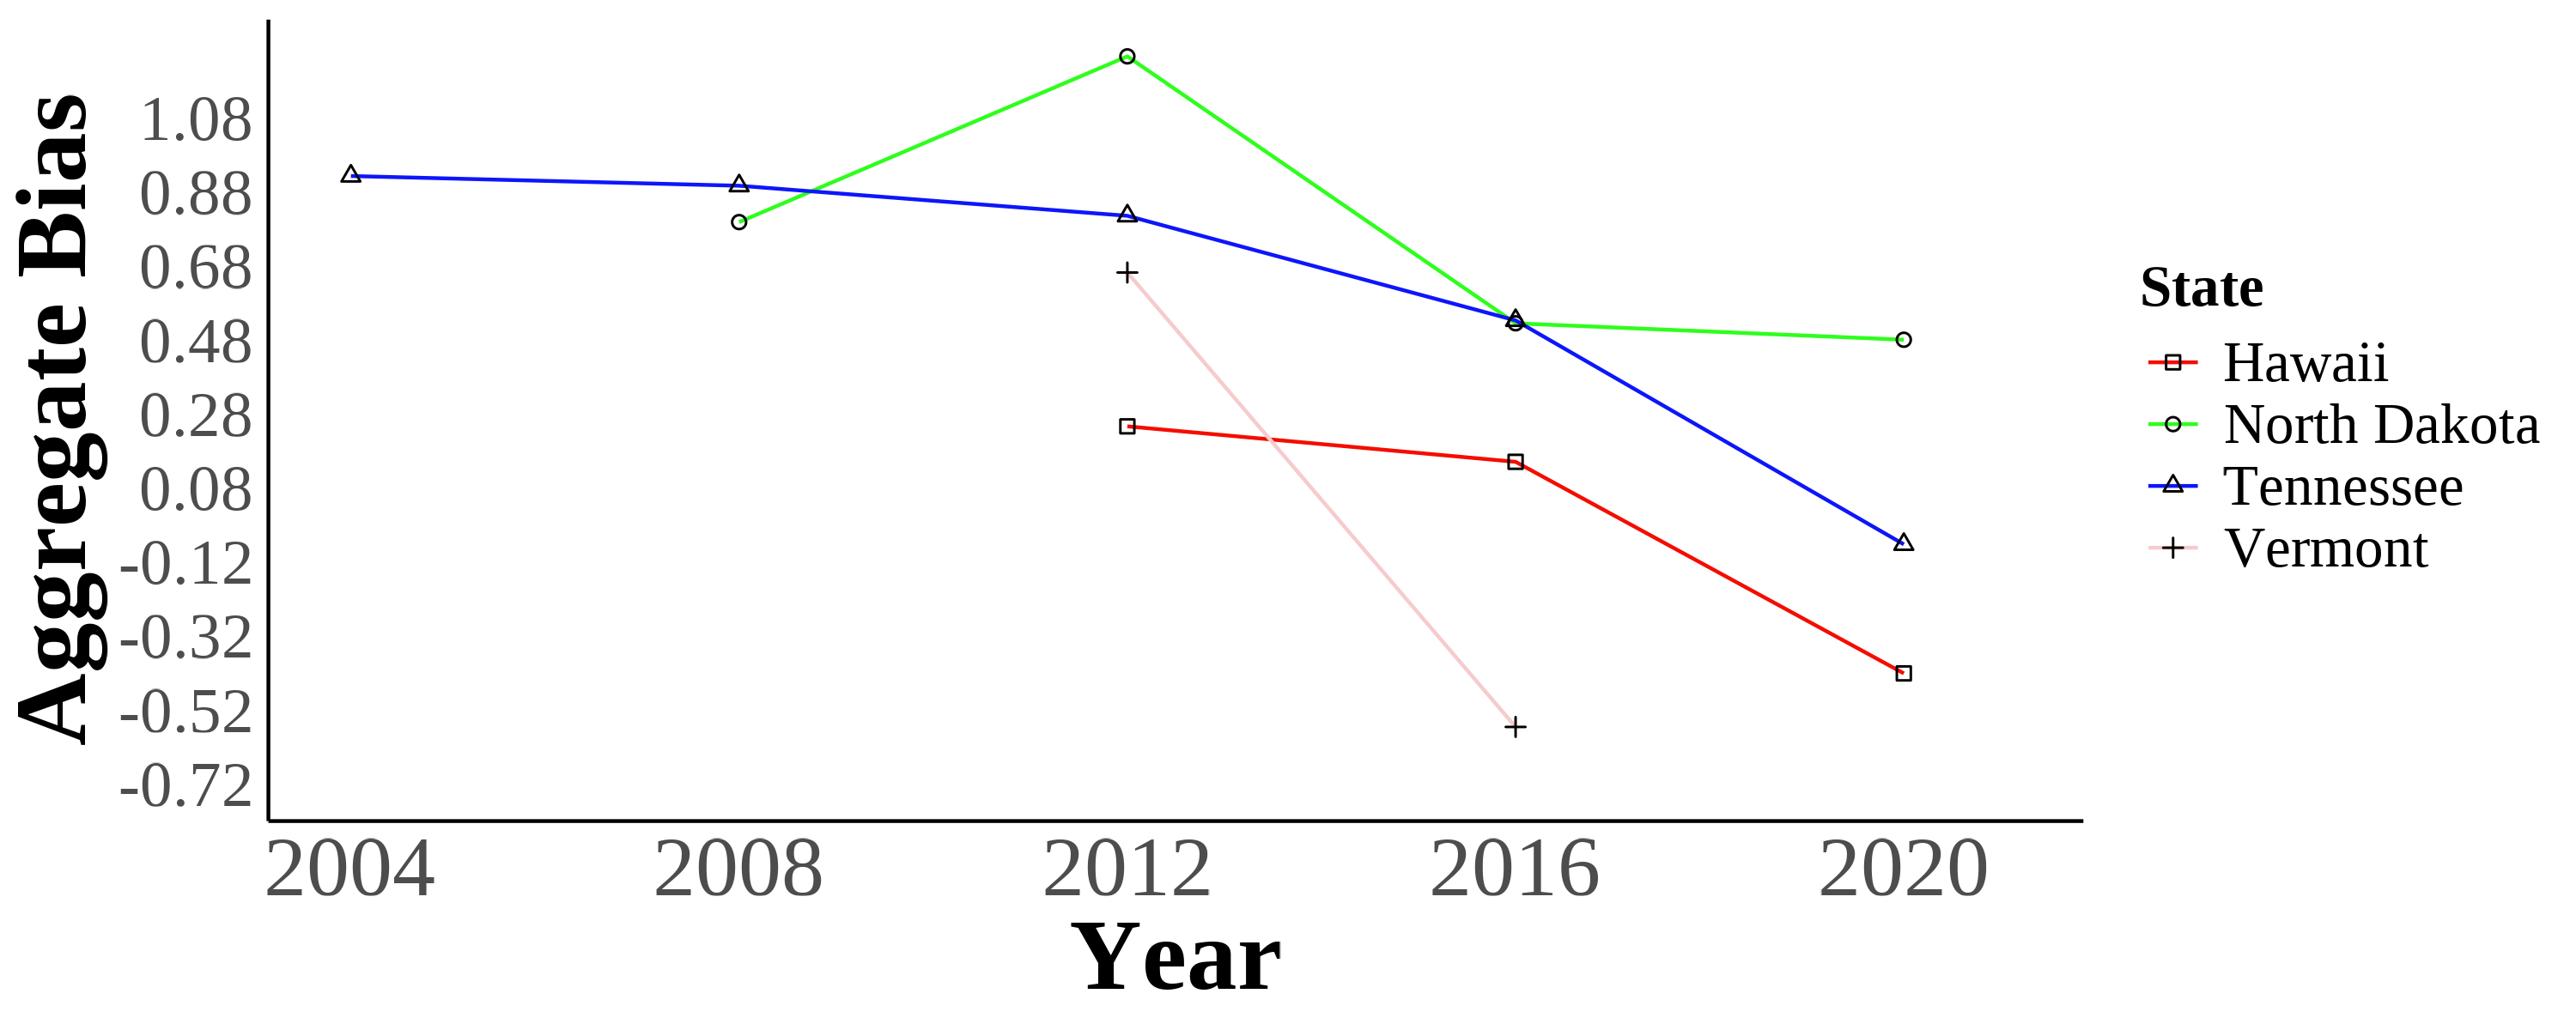
\includegraphics[width=.9\linewidth]{Bias_twostates.png} 
\label{fig:skiniat}
\end{subfigure}
% Second
\begin{subfigure}{.9\textwidth}
\caption{Self-reported Asian Identity Over Time}
\centering
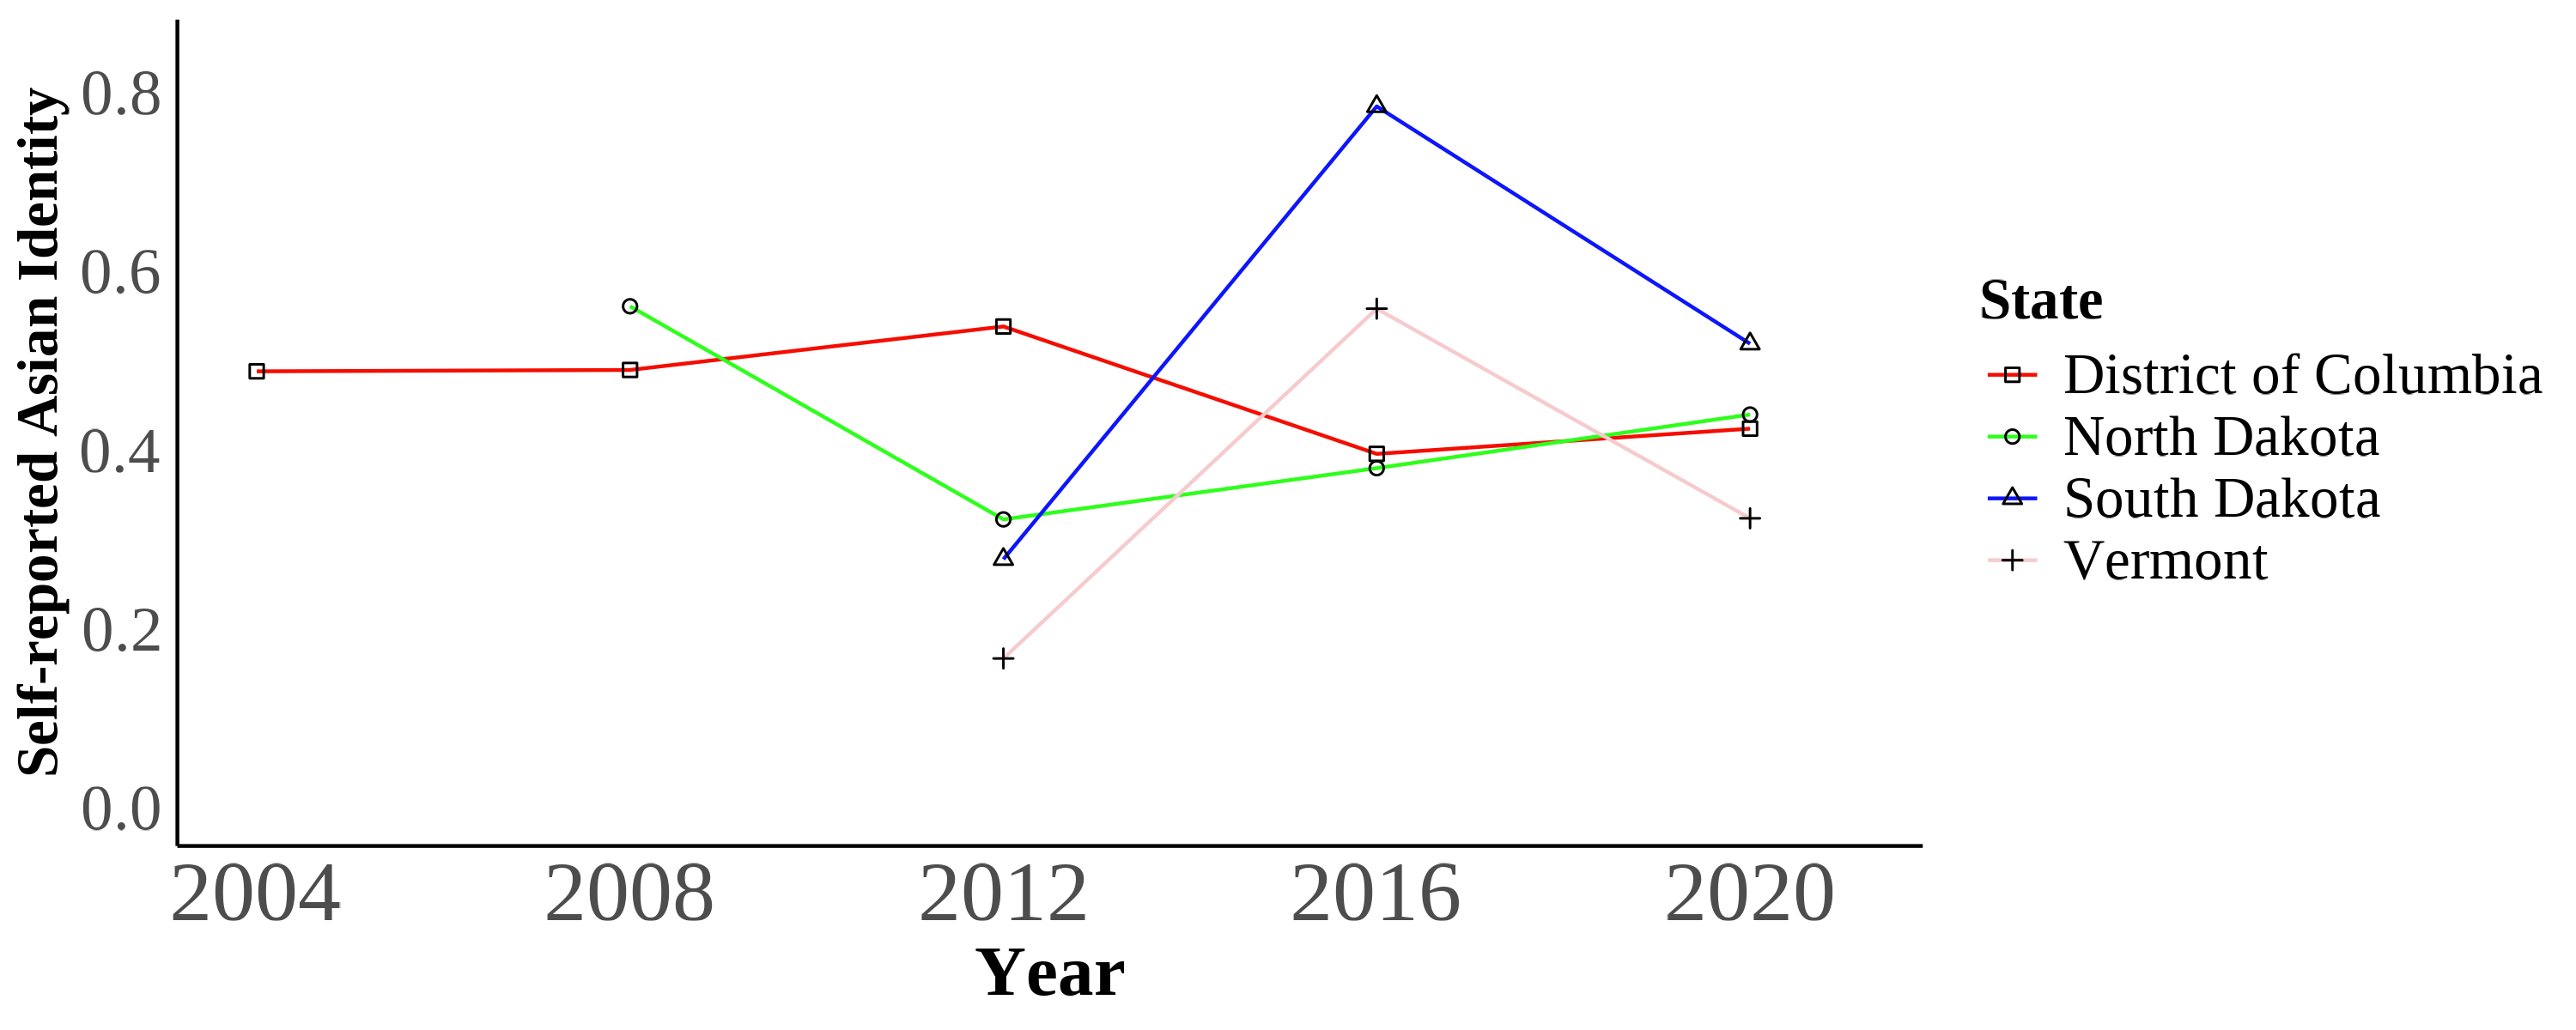
\includegraphics[width=.9\linewidth]{Bias_twostates-asian.png} 
\label{fig:Asian-twostates}
\end{subfigure}
\caption*{\footnotesize{These two panels show the trends in bias (panel a) and self-reported Asian identity among Asian immigrants (panel b) of the least and most biased places in the data. The District of Colombia is the least biased geographical area, and North Dakota is the most biased. The bias units are in standard deviations. Self-reported Asian identity is among first, second, and third-generation Asian immigrants aged 17 and younger still living in intact families.\\
Bias data is from the 2004-2021 Harvard's Project Implicit Association Test scores, American National Election Studies (ANES), and state-level hate crimes against Asians. Identity data is from the 2004-2021 Current Population Survey (CPS).}}
\end{figure}
\end{center}


\newpage
\pagebreak

\begin{center}
\begin{figure}[H]
\caption{Diagram of the Three Different Generations of Asian Immigrants.}
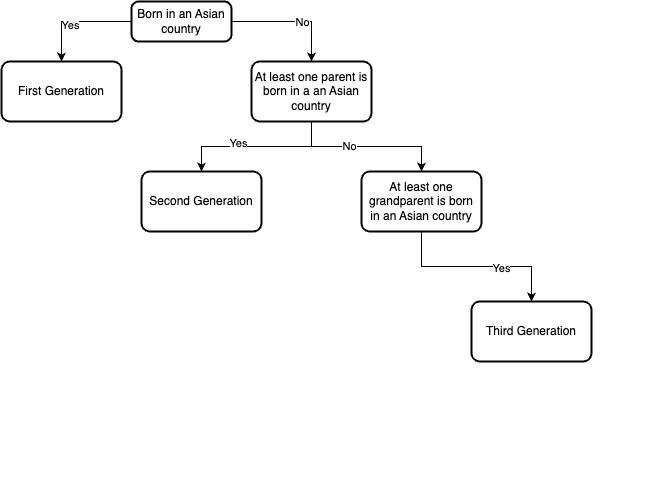
\includegraphics[width=\textwidth, height=9cm]{diag.png} 
\label{fig:diag}
\end{figure}
\hfill%
\end{center}

\pagebreak
\newpage

\begin{center}
\begin{figure}[H]
\caption{Maps of State-level Association Test Bias Over Time Measure with Census Division Regional Boundaries}
\label{fig:skiniat-maps}
% first
\begin{subfigure}{.45\textwidth}
\caption{State-level Bias in 2004}
\centering
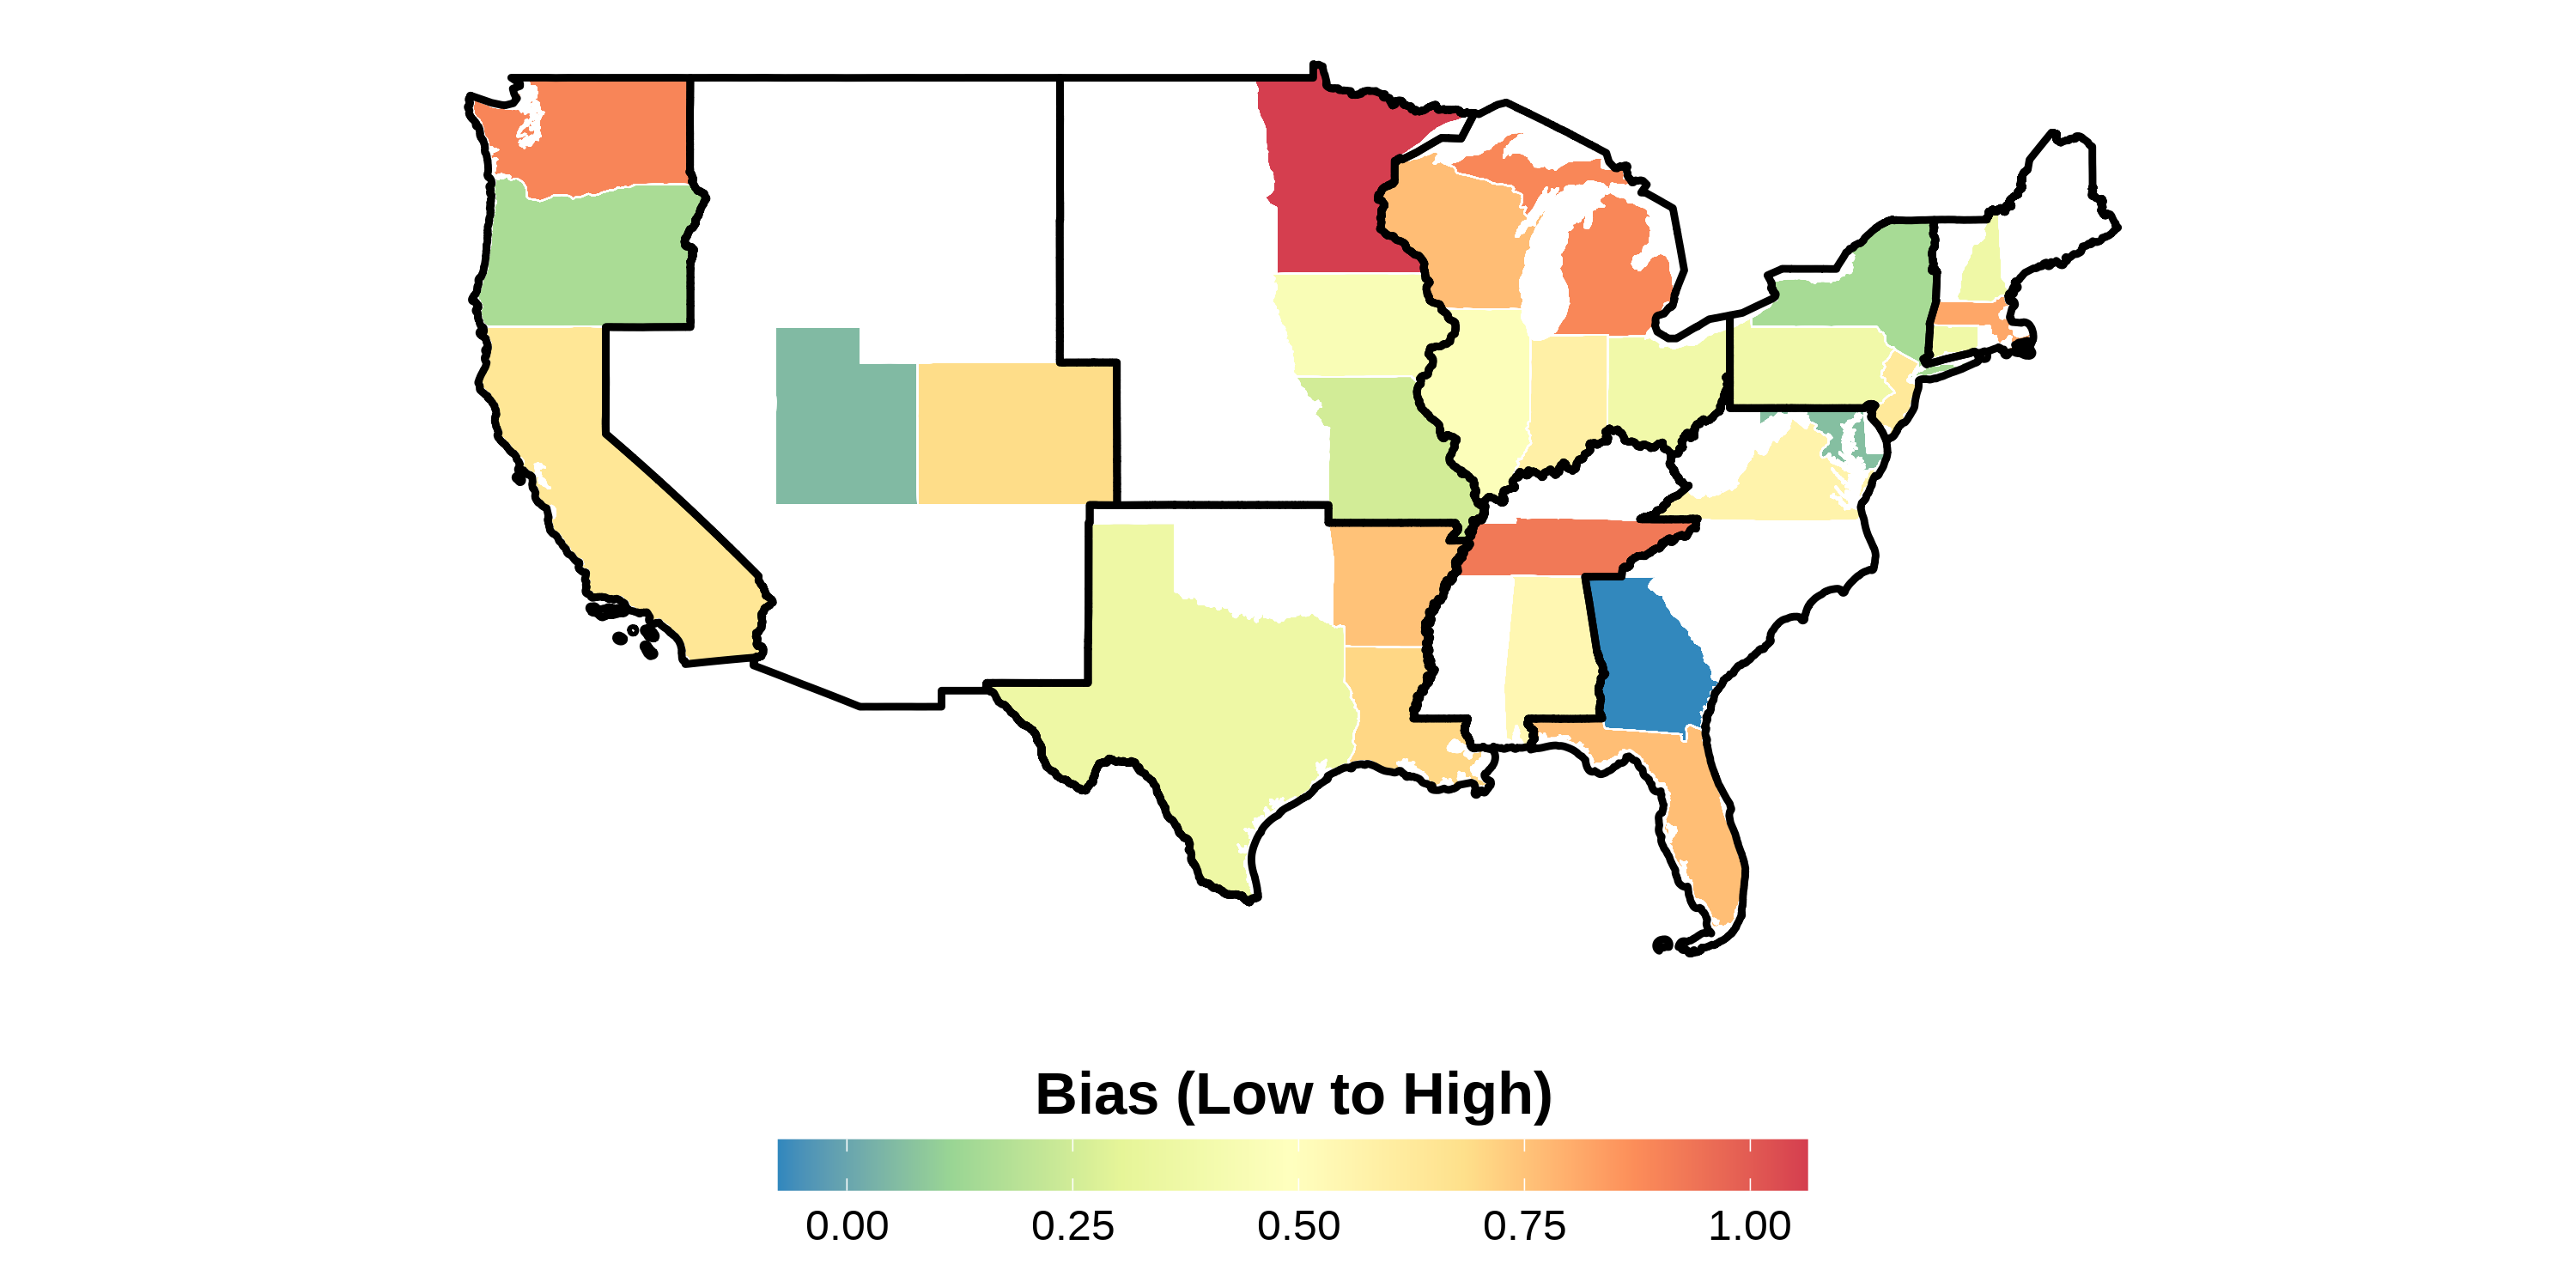
\includegraphics[width=0.9\linewidth]{2004skinmap.png} 
\label{fig:skiniat-map-2004}
\end{subfigure}
\hfill%
% Second
\begin{subfigure}{.45\textwidth}
\caption{State-level Bias in 2008}
\centering
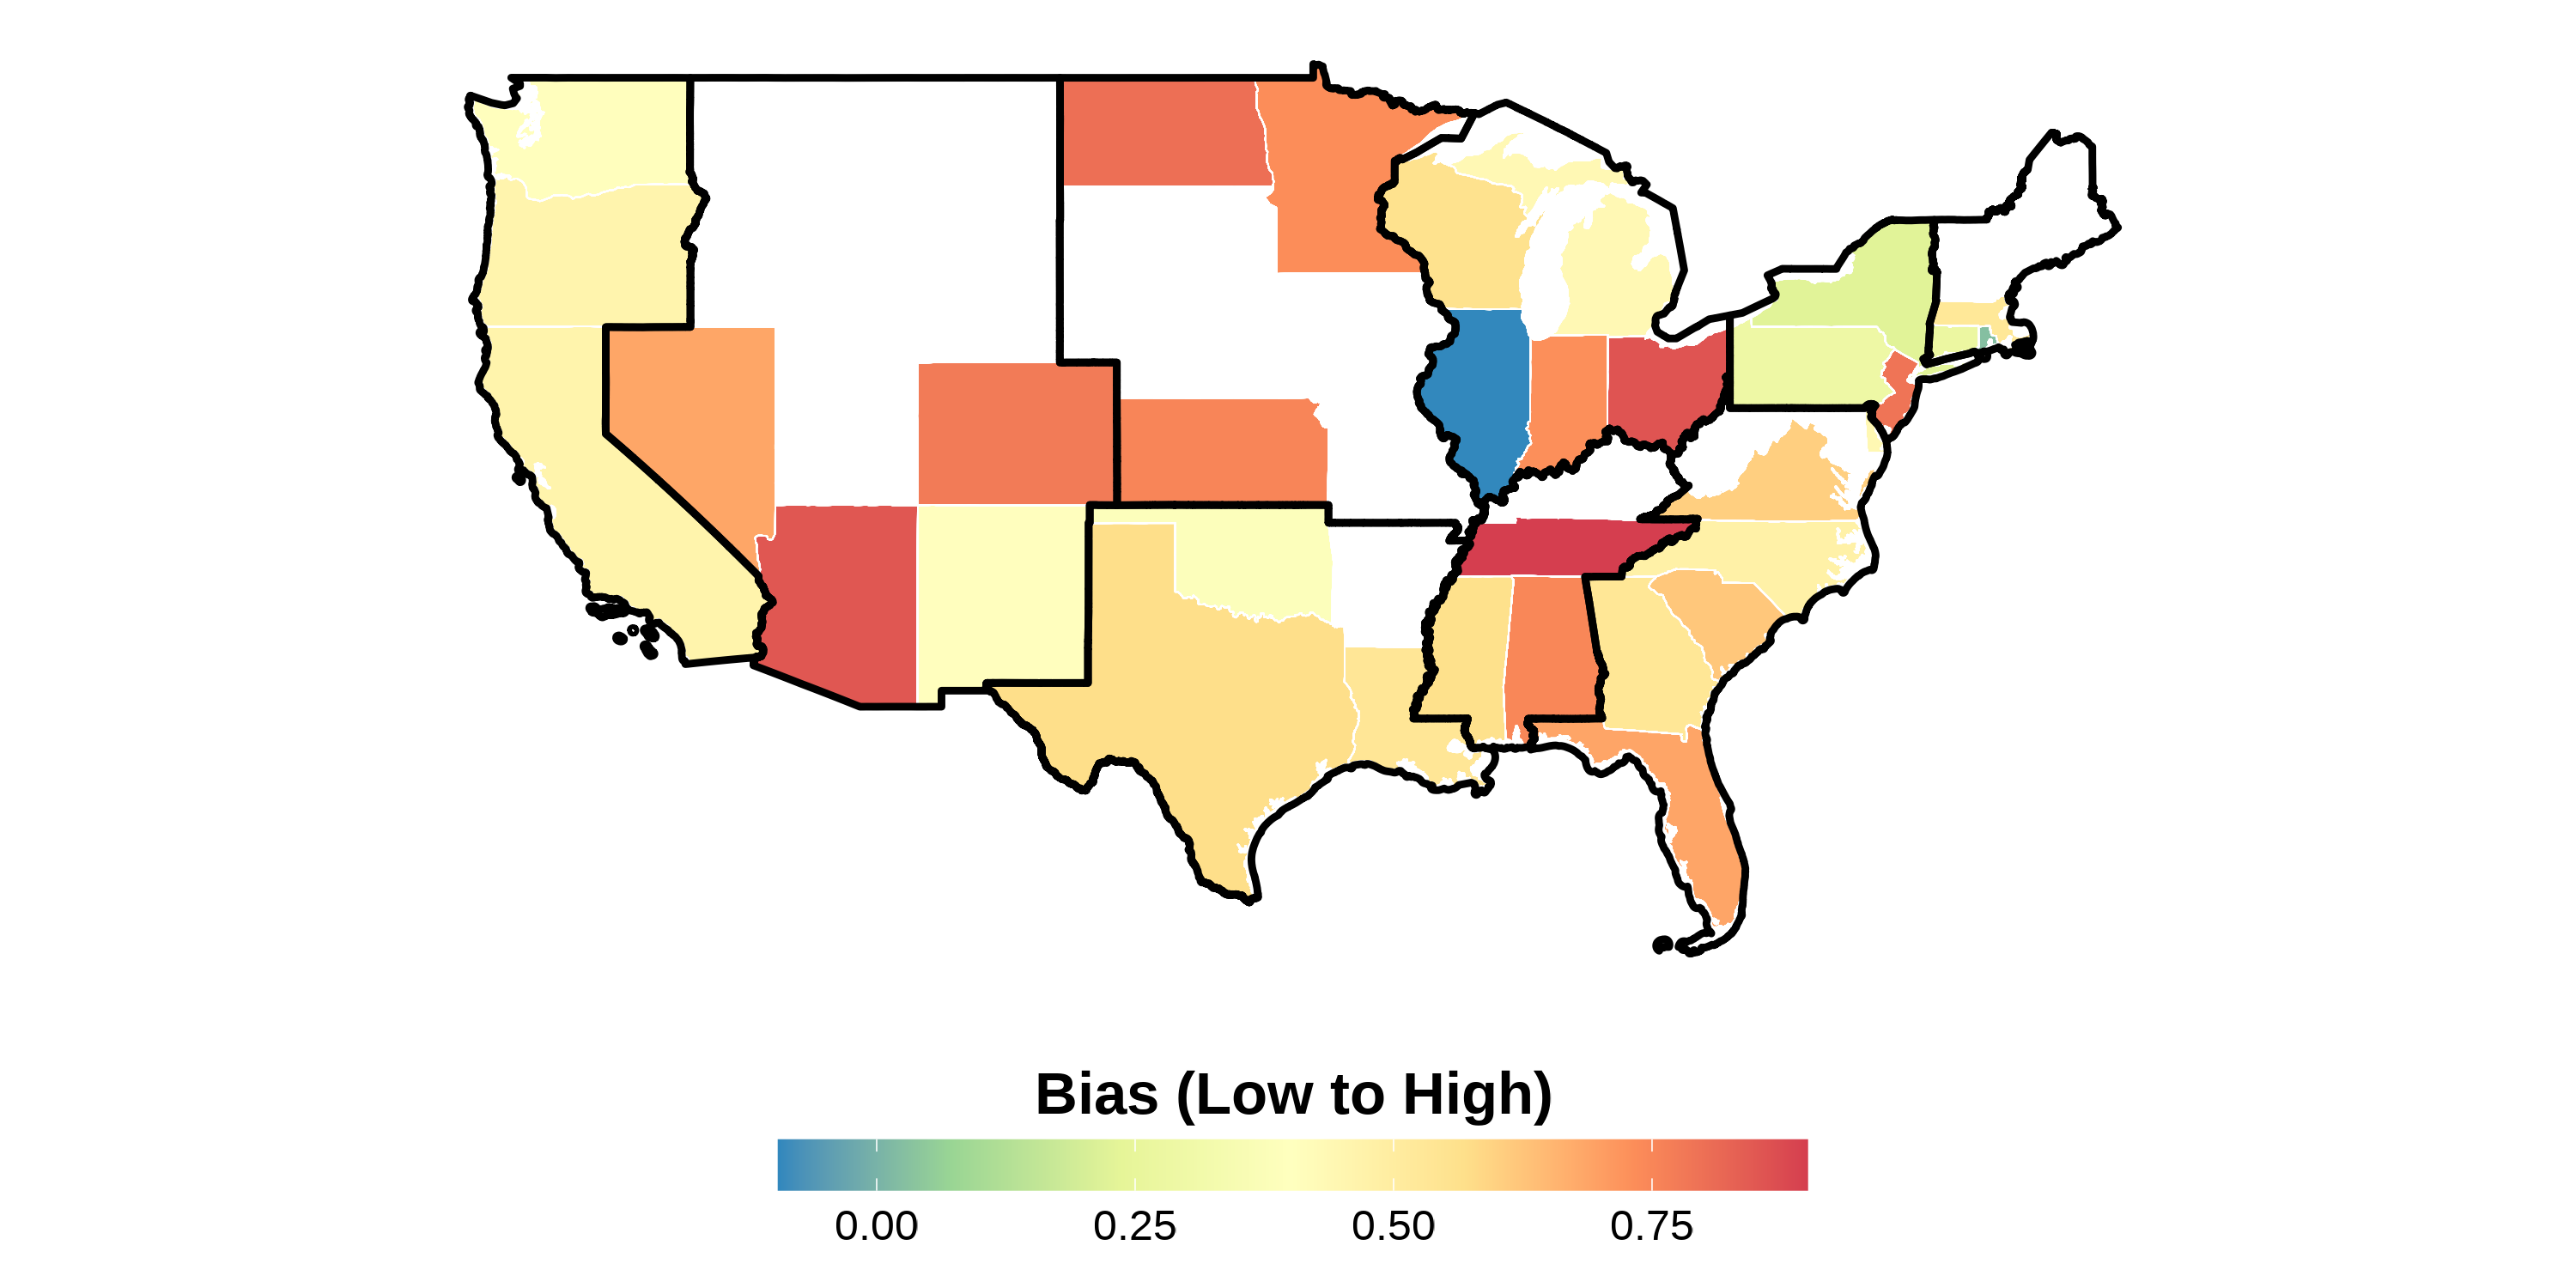
\includegraphics[width=0.9\linewidth]{2008skinmap.png} 
\label{fig:skiniat-map-2006}
\end{subfigure}
\hfill%
% third
\begin{subfigure}{.45\textwidth}
\caption{State-level Bias in 2012}
\centering
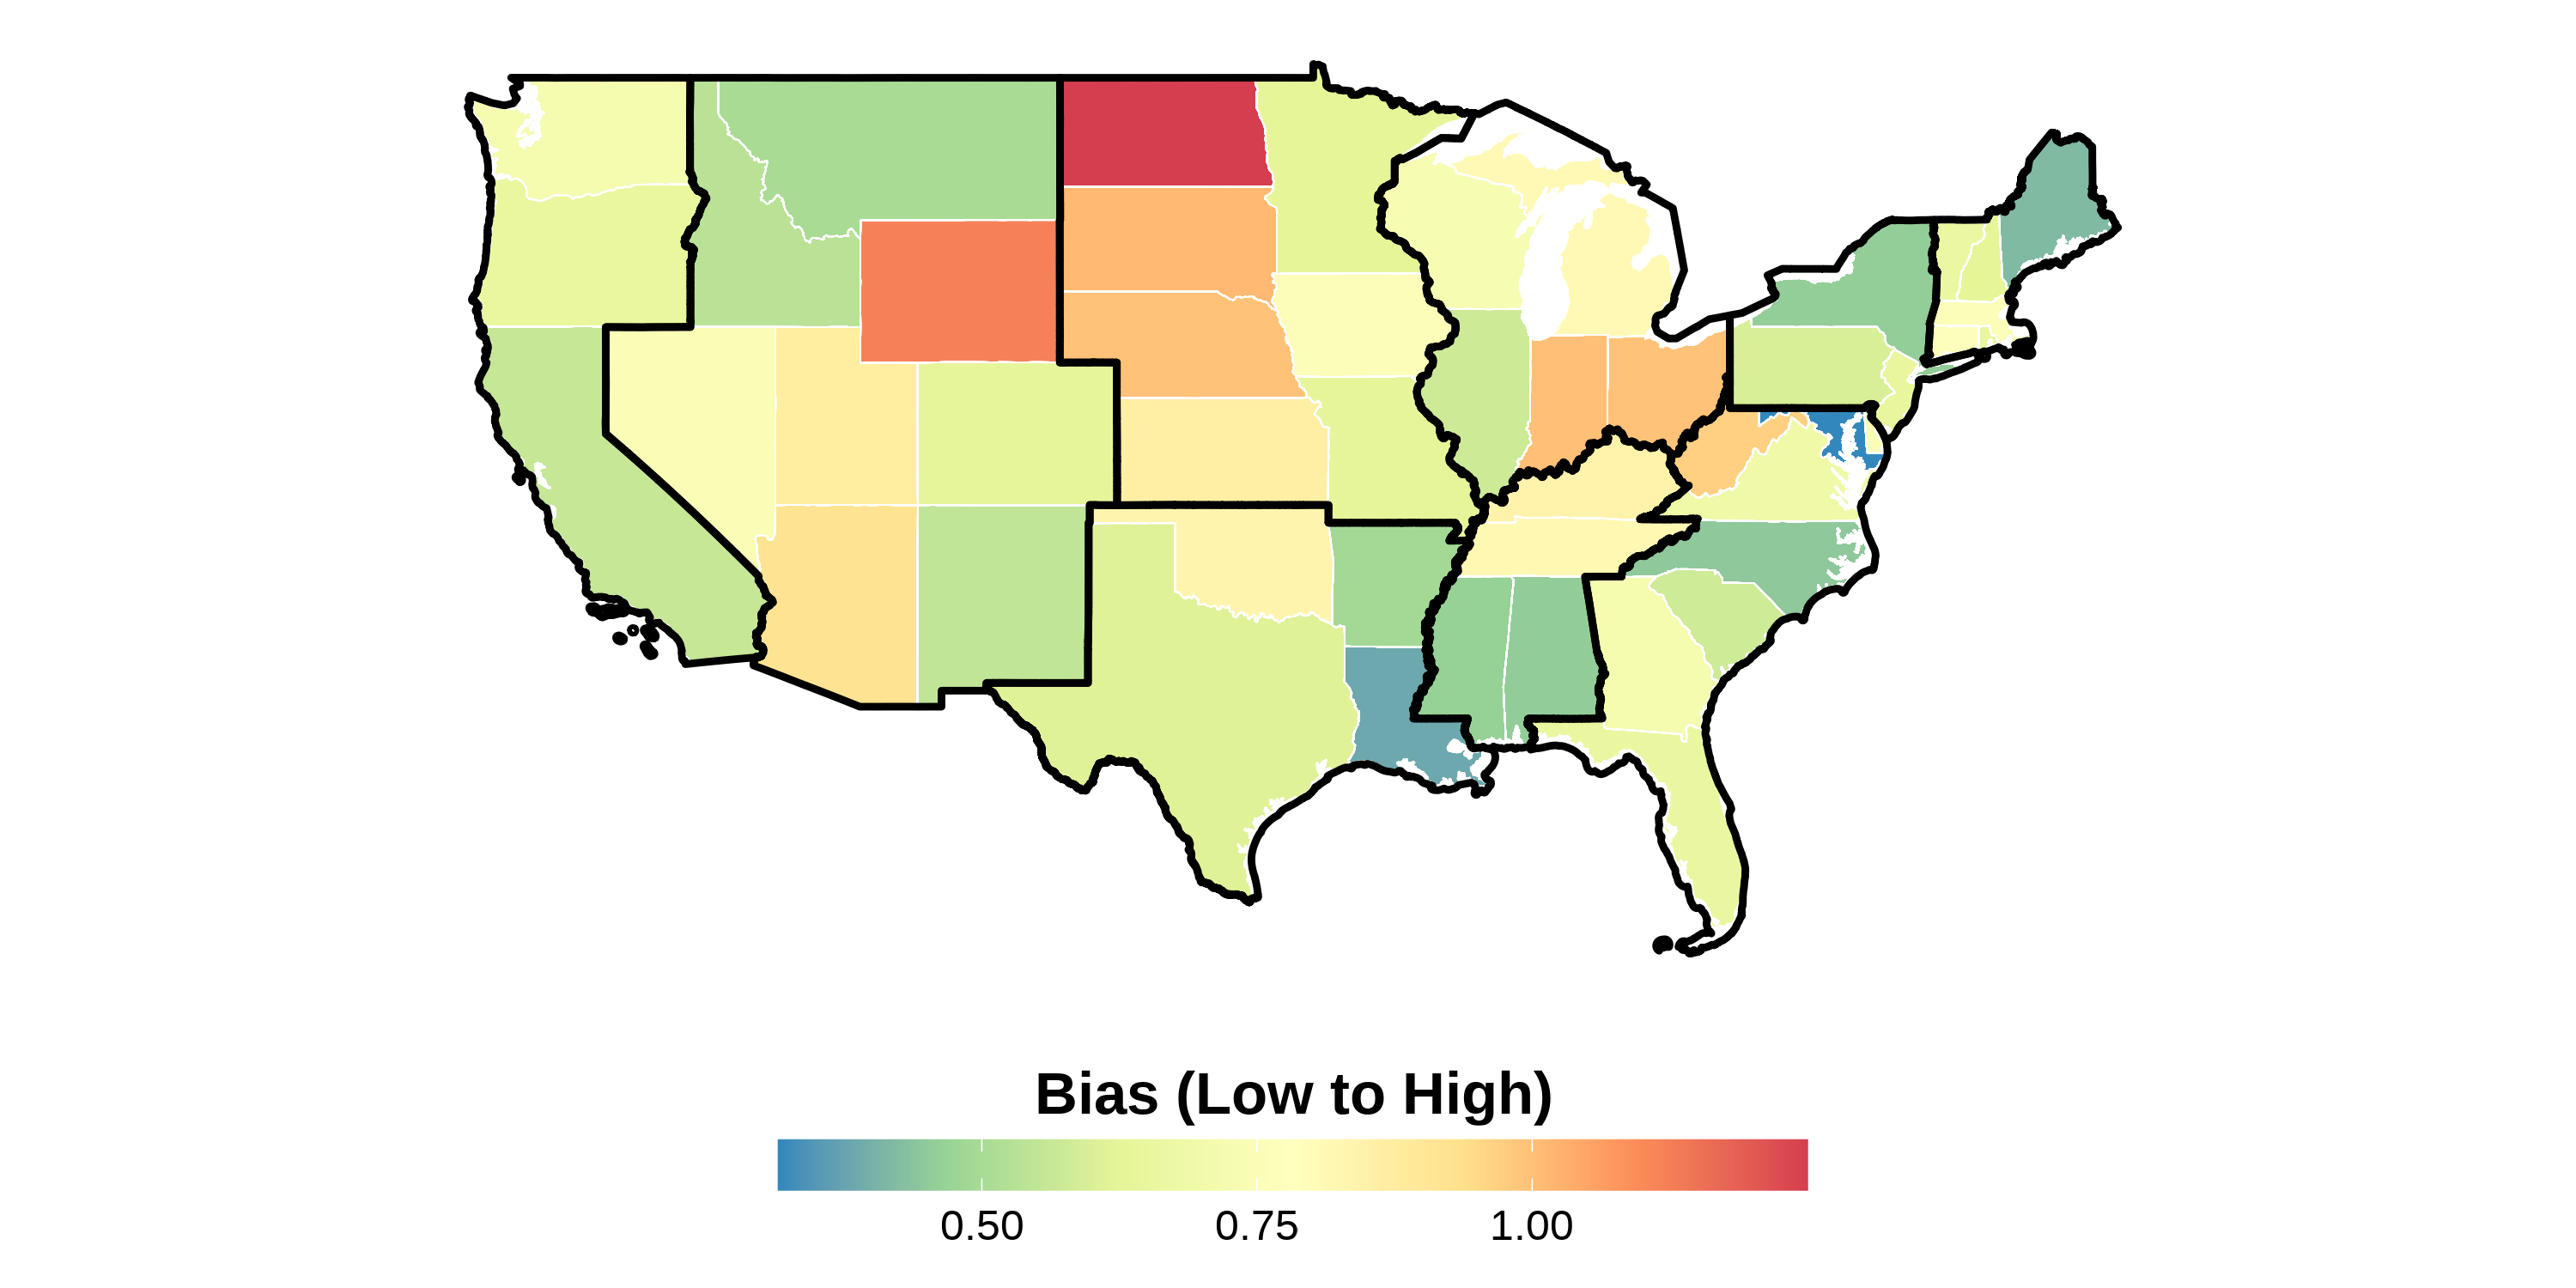
\includegraphics[width=0.9\linewidth]{2012skinmap.png} 
\label{fig:skiniat-map-2008}
\end{subfigure}
\hfill%
% fourth
\begin{subfigure}{.45\textwidth}
\caption{State-level Bias in 2016}
\centering
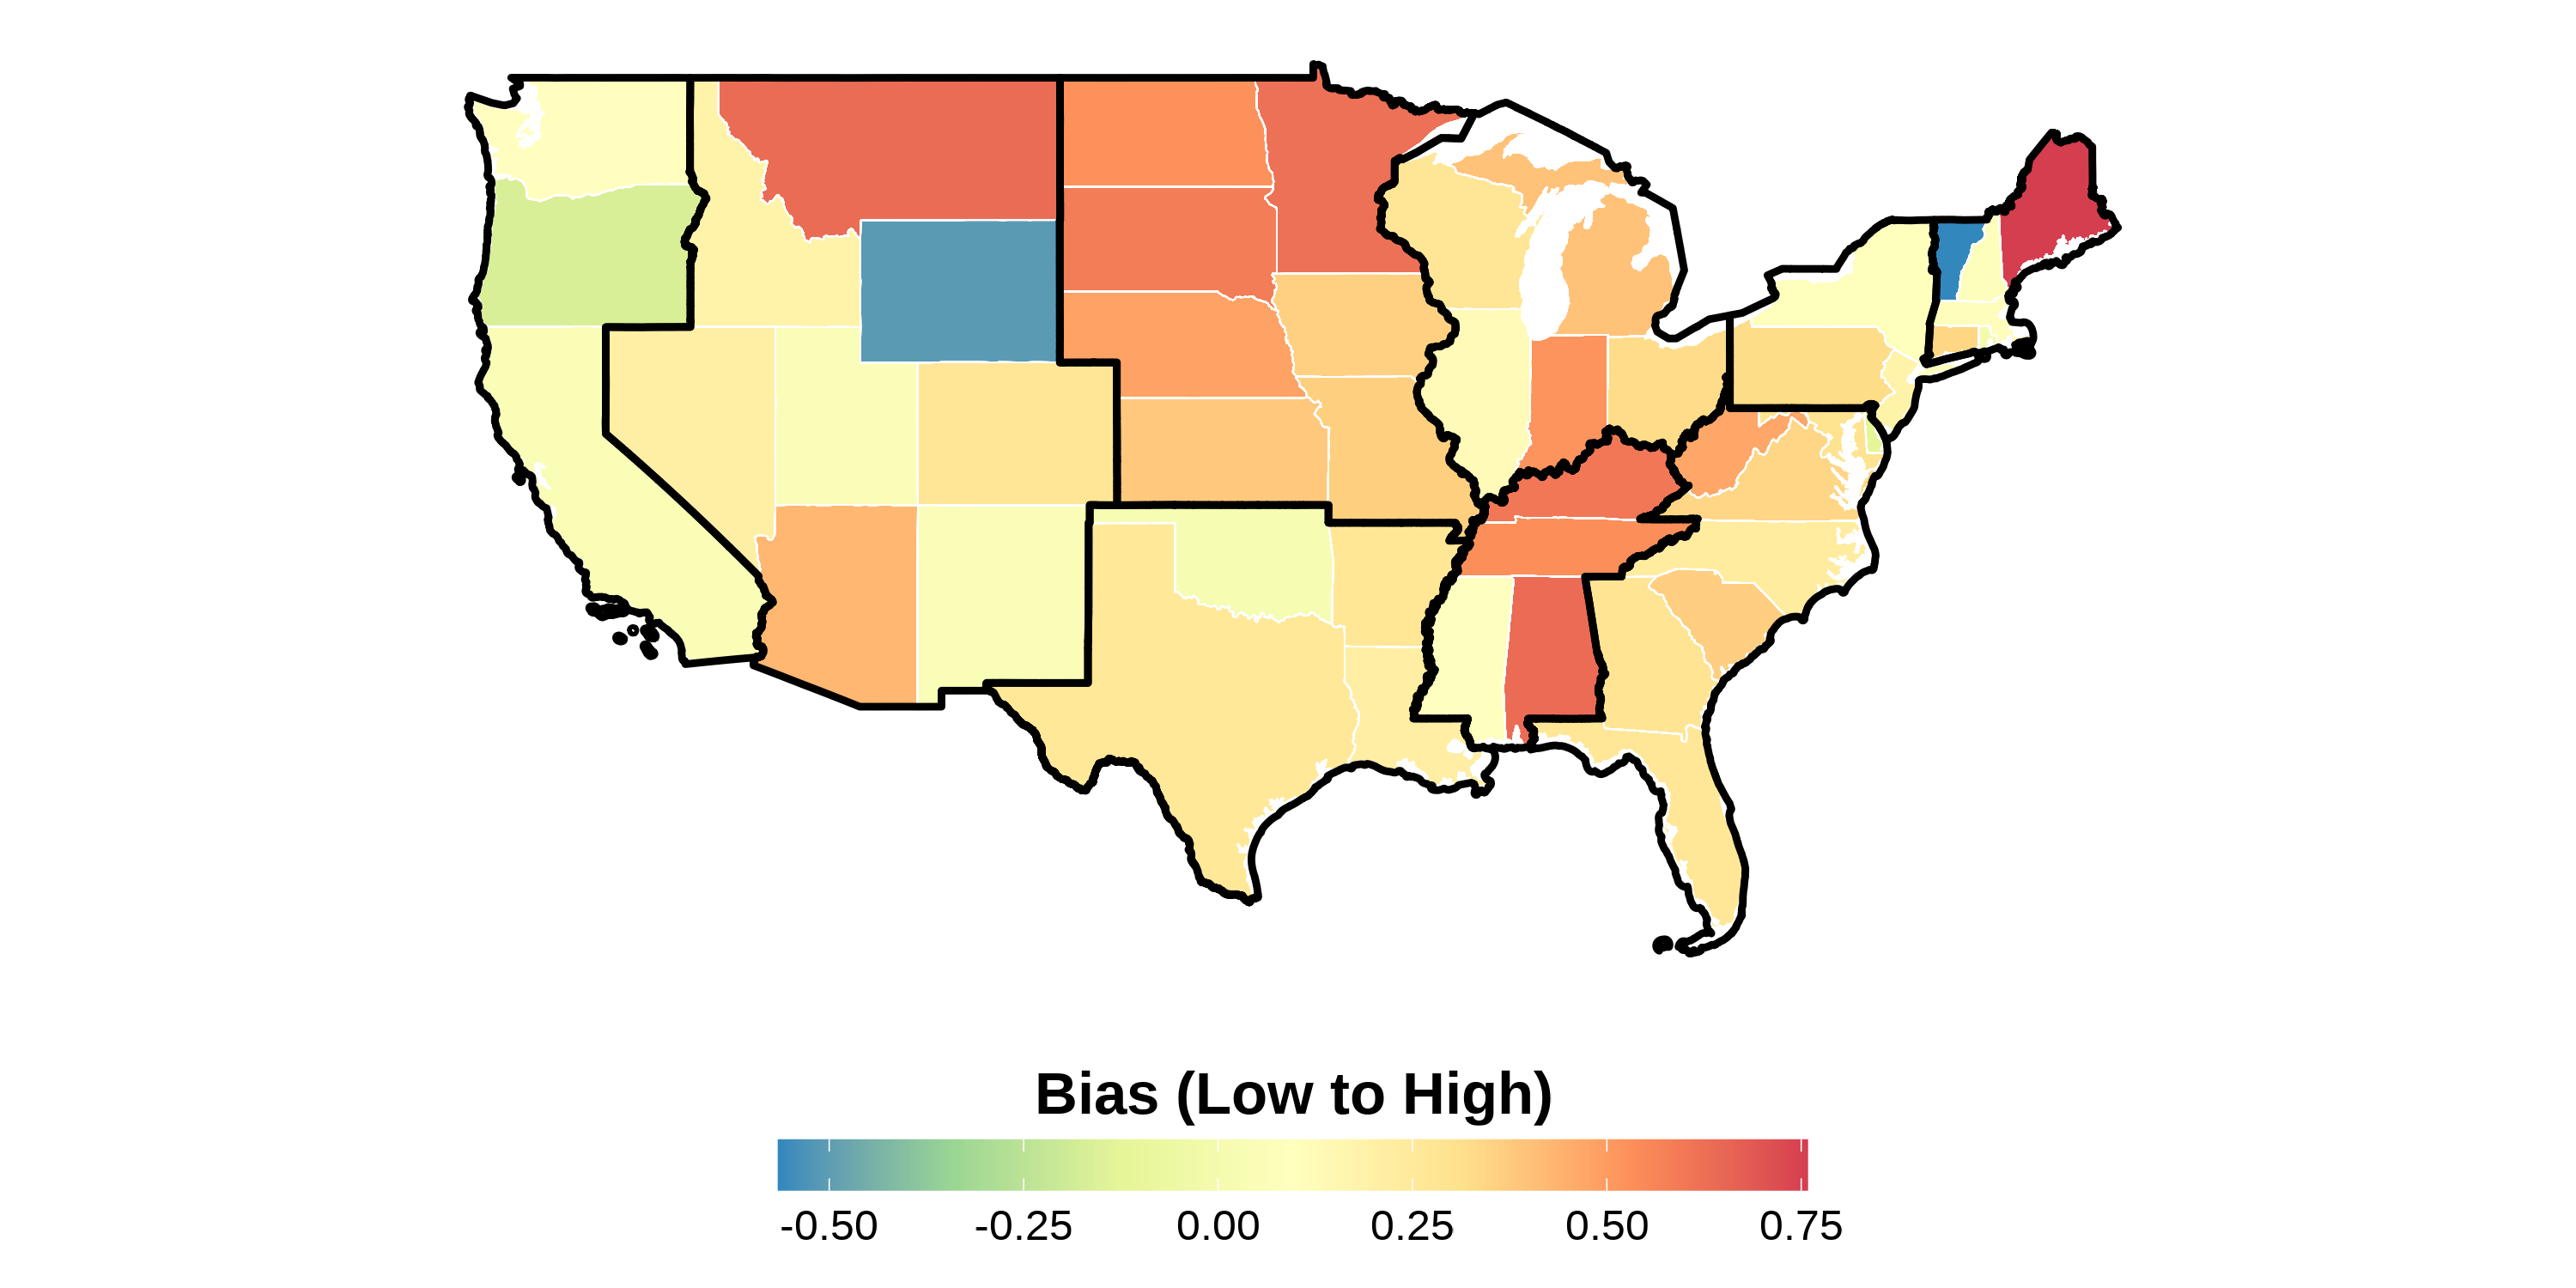
\includegraphics[width=0.9\linewidth]{2016skinmap.png} 
\label{fig:skiniat-map-2010}
\end{subfigure}

\caption*{\footnotesize{This figure shows the state-level bias index in different years in the sample. The bias units are in standard deviations and ranges from low to high bias. Bias index is constructed following \textcite{lubotskyInterpretationRegressionsMultiple2006}. The data is from the 2004-2021 Harvard's Project Implicit Association Test scores, American National Election Studies (ANES), and state-level hate crimes against Asians. Each panel presents state-level bias during a certain year. The boundaries in black represent the different Census divisions in the United States. Notice how there is a variation across states within a region.}}
\end{figure}
\end{center}

\newpage
\pagebreak

\begin{center}
\begin{figure}[H]
\caption{Maps of State-level Bias 2004-2021 Measure with Census Division Regional Boundaries}
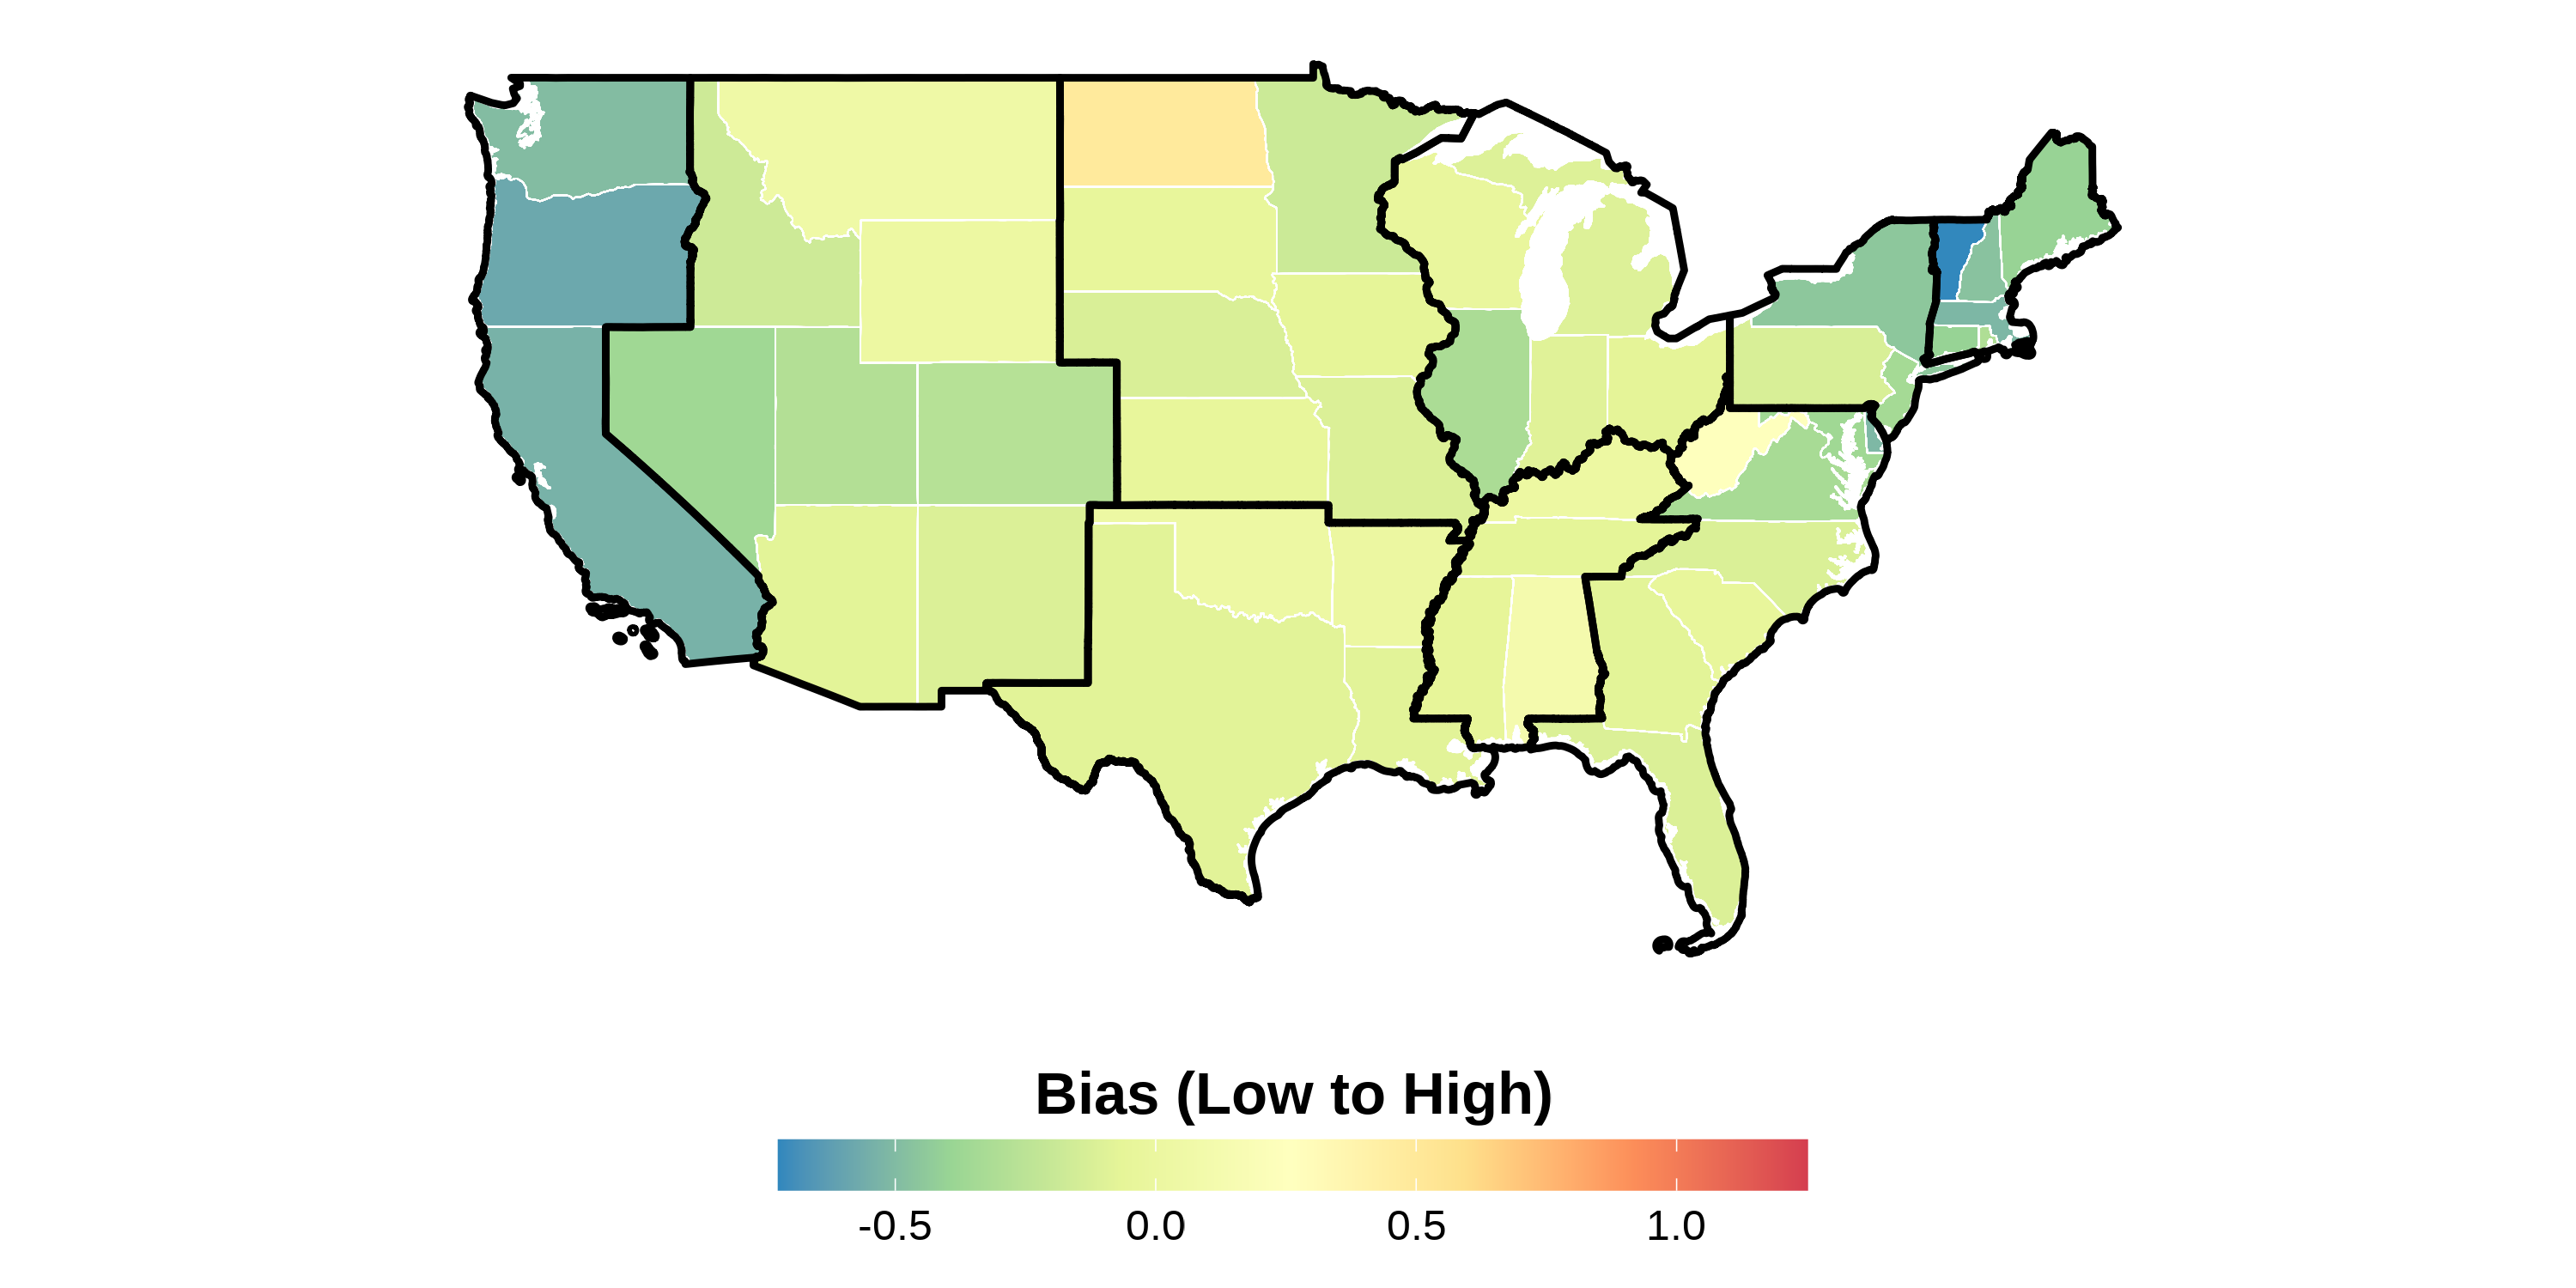
\includegraphics[width=\textwidth]{Average_Skinmap.png} 
\label{fig:iat-map-all}
\caption*{\footnotesize{This figure shows the state-level bias index in the sample from 2004 to 2021. The bias units are in standard deviations and ranges from low to high bias. Bias index is constructed following \textcite{lubotskyInterpretationRegressionsMultiple2006}. The data is from the 2004-2021 Harvard's Project Implicit Association Test scores, American National Election Studies (ANES), and state-level hate crimes against Asians. The boundaries in black represent the different Census divisions in the United States. Notice how there is a variation across states within a region.}}
\end{figure}
\end{center}

\newpage
\pagebreak

\begin{center}
\begin{figure}[H]
\caption{Asian Racial Identity}
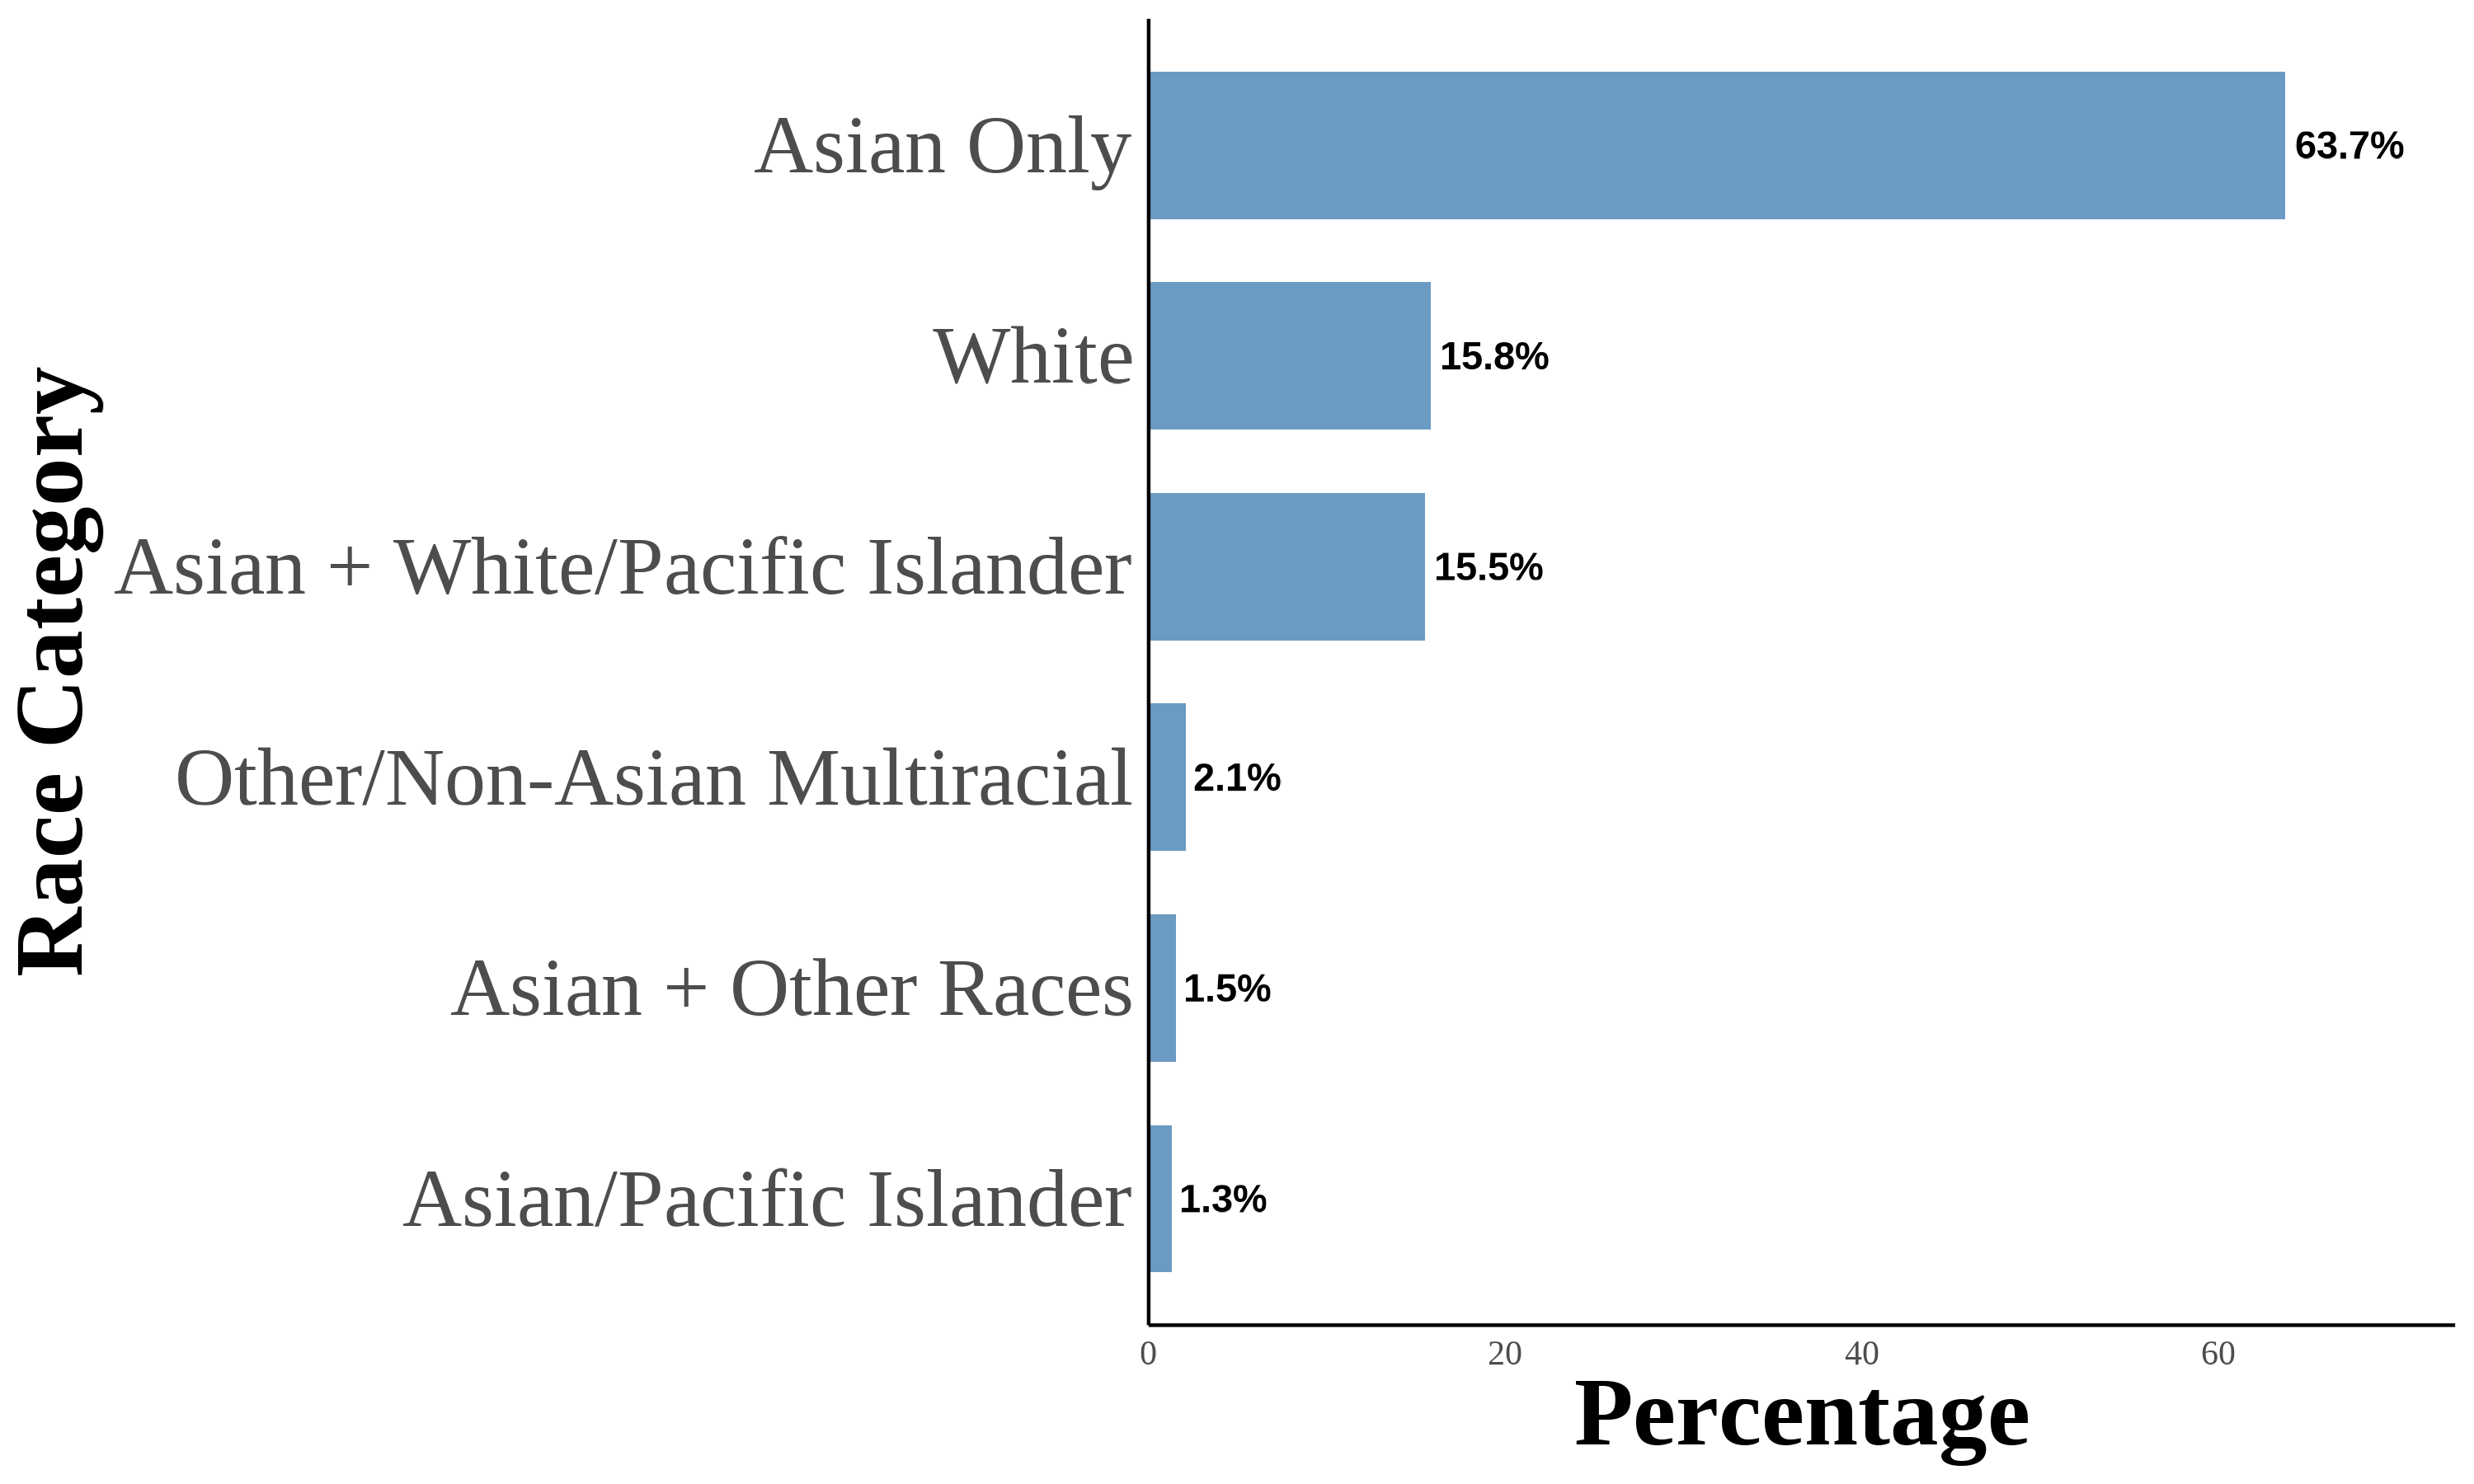
\includegraphics[width=\textwidth]{histogram_asian_american_race_aggregated.png} 
\label{fig:histogram-all}
\caption*{\footnotesize{This figure shows the distribution of Asian racial identity among respondents. 
The data is aggregated from the 2004-2021 Current Population Survey (CPS). 
The sample includes first-, second-, and third-generation objectively Asian Americans.
Following \textcite{antmanEthnicAttritionObserved2016,antmanEthnicAttritionAssimilation2020}, 
I utilize birthplace information for individuals, parents, and grandparents to create objective Asian ancestry indicators.
}}
\end{figure}
\end{center}

\newpage
\pagebreak

\begin{center}
\begin{figure}[H]
\caption{Asian Racial Identity: First Generation}
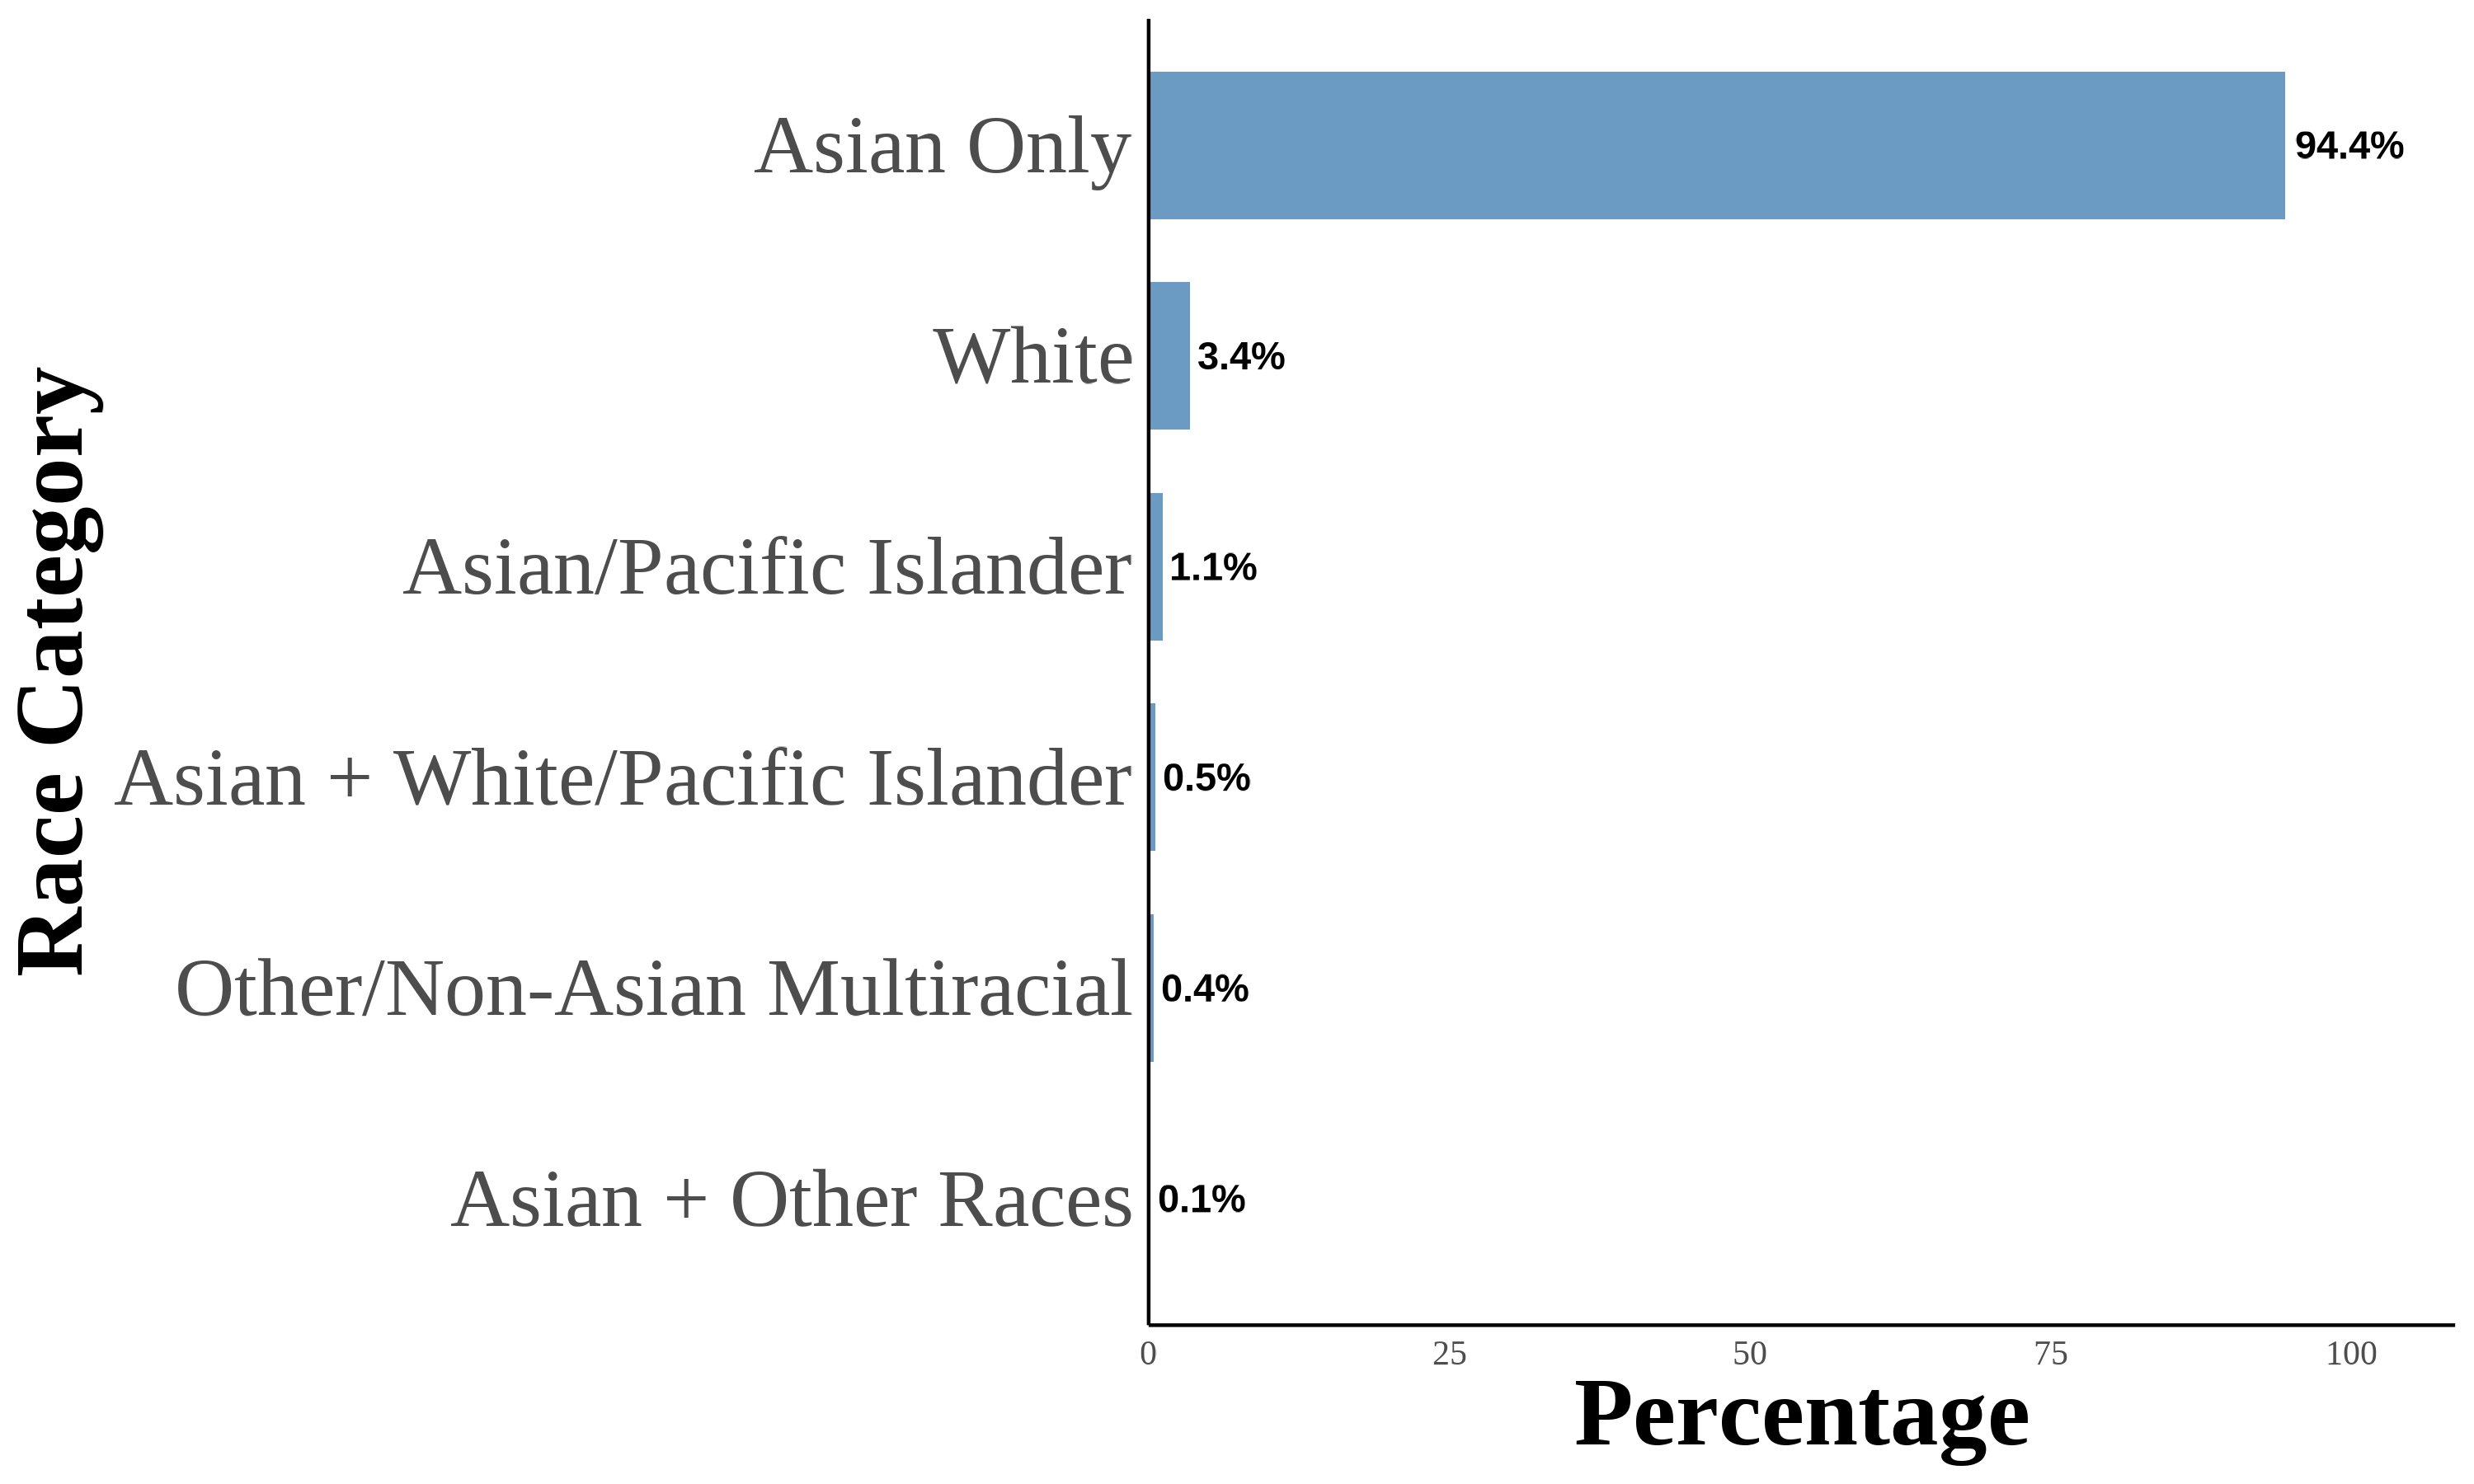
\includegraphics[width=\textwidth]{histogram_asian_american_race_firstgen.png} 
\label{fig:histogram-firstgen}
\caption*{\footnotesize{This figure shows the distribution of Asian racial identity among respondents. 
The data is aggregated from the 2004-2021 Current Population Survey (CPS). 
The sample includes first-generation objectively Asian Americans.
Following \textcite{antmanEthnicAttritionObserved2016,antmanEthnicAttritionAssimilation2020}, 
I utilize birthplace information for individuals, parents, and grandparents to create objective Asian ancestry indicators.
A first-generation Asian American is defined as an individual born in an Asian country and is not a US citizen born to US citizen parents abroad.
}}
\end{figure}
\end{center}


\pagebreak
\newpage

\begin{landscape}
\begin{figure}[!htb]
\centering
\caption{Asian Racial Identity: Second Generation}
\label{fig:histogram-secondgen}

% Top row
\begin{subfigure}{.48\textwidth}
\caption{All Second Generation}
\centering
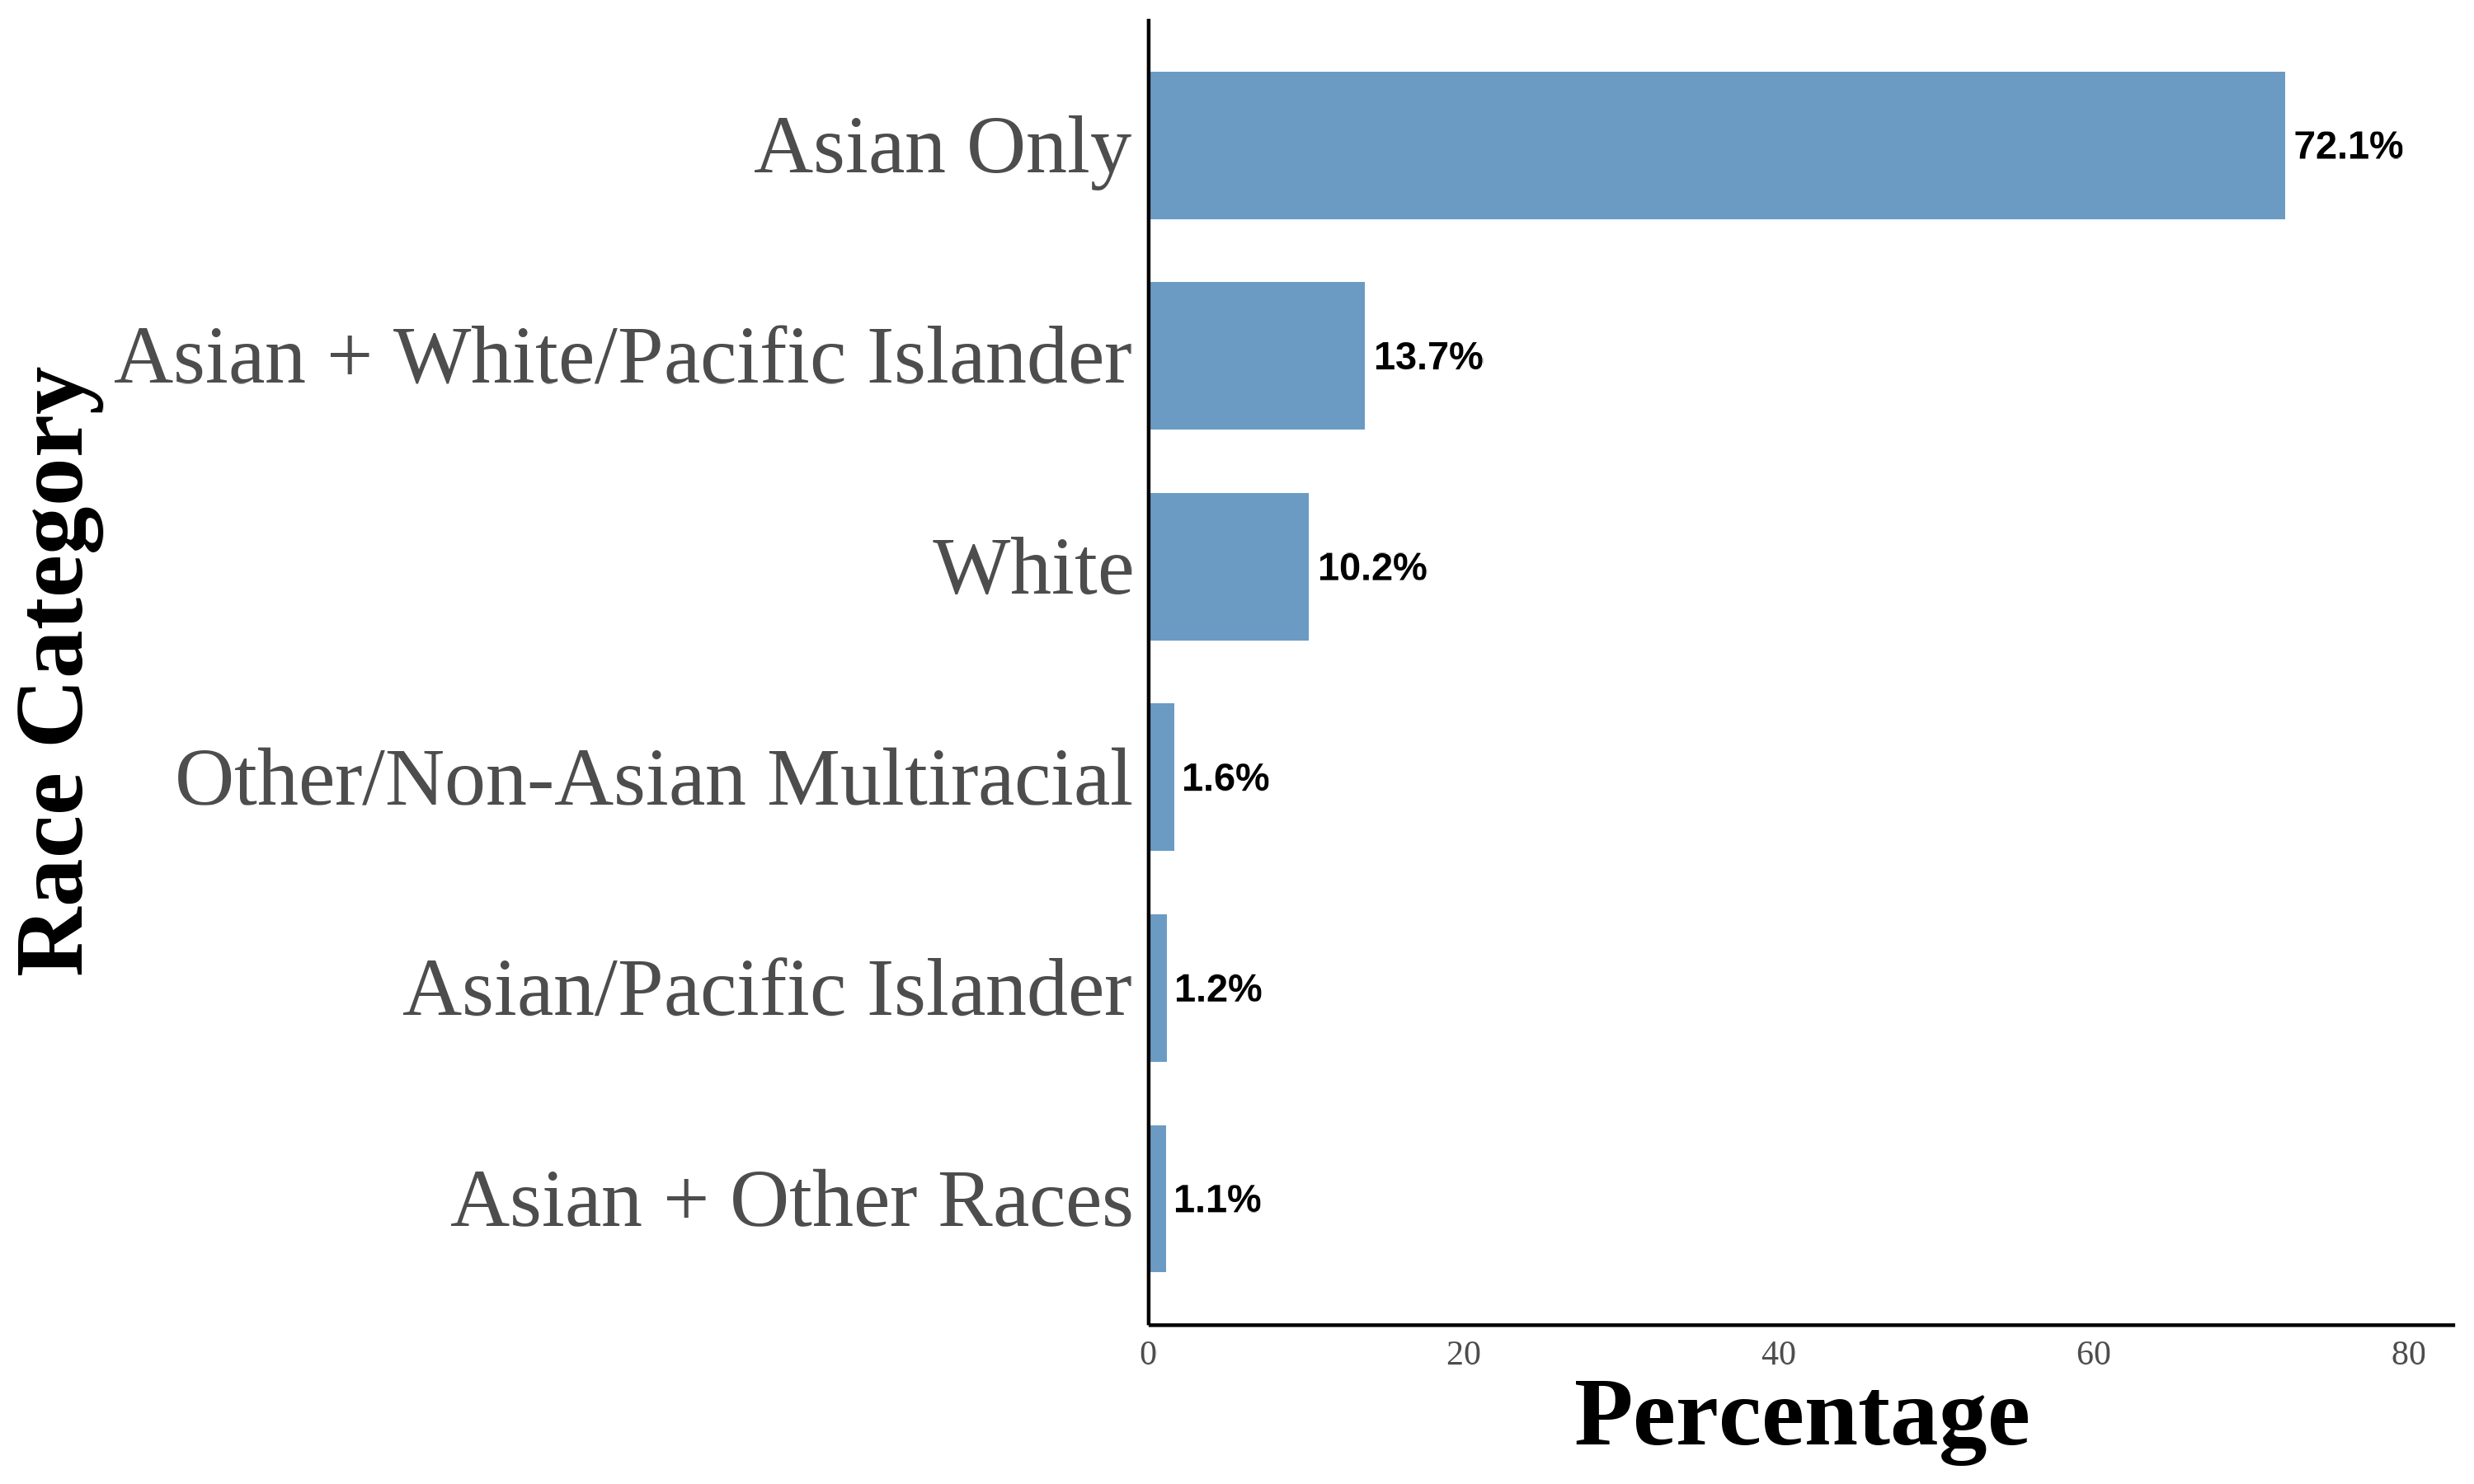
\includegraphics[width=1\linewidth]{histogram_asian_american_race_secondgen.png}
\end{subfigure}
\hfill
\begin{subfigure}{.48\textwidth}
\caption{Second Generation: Asian Fathers-Asian Mothers}
\centering
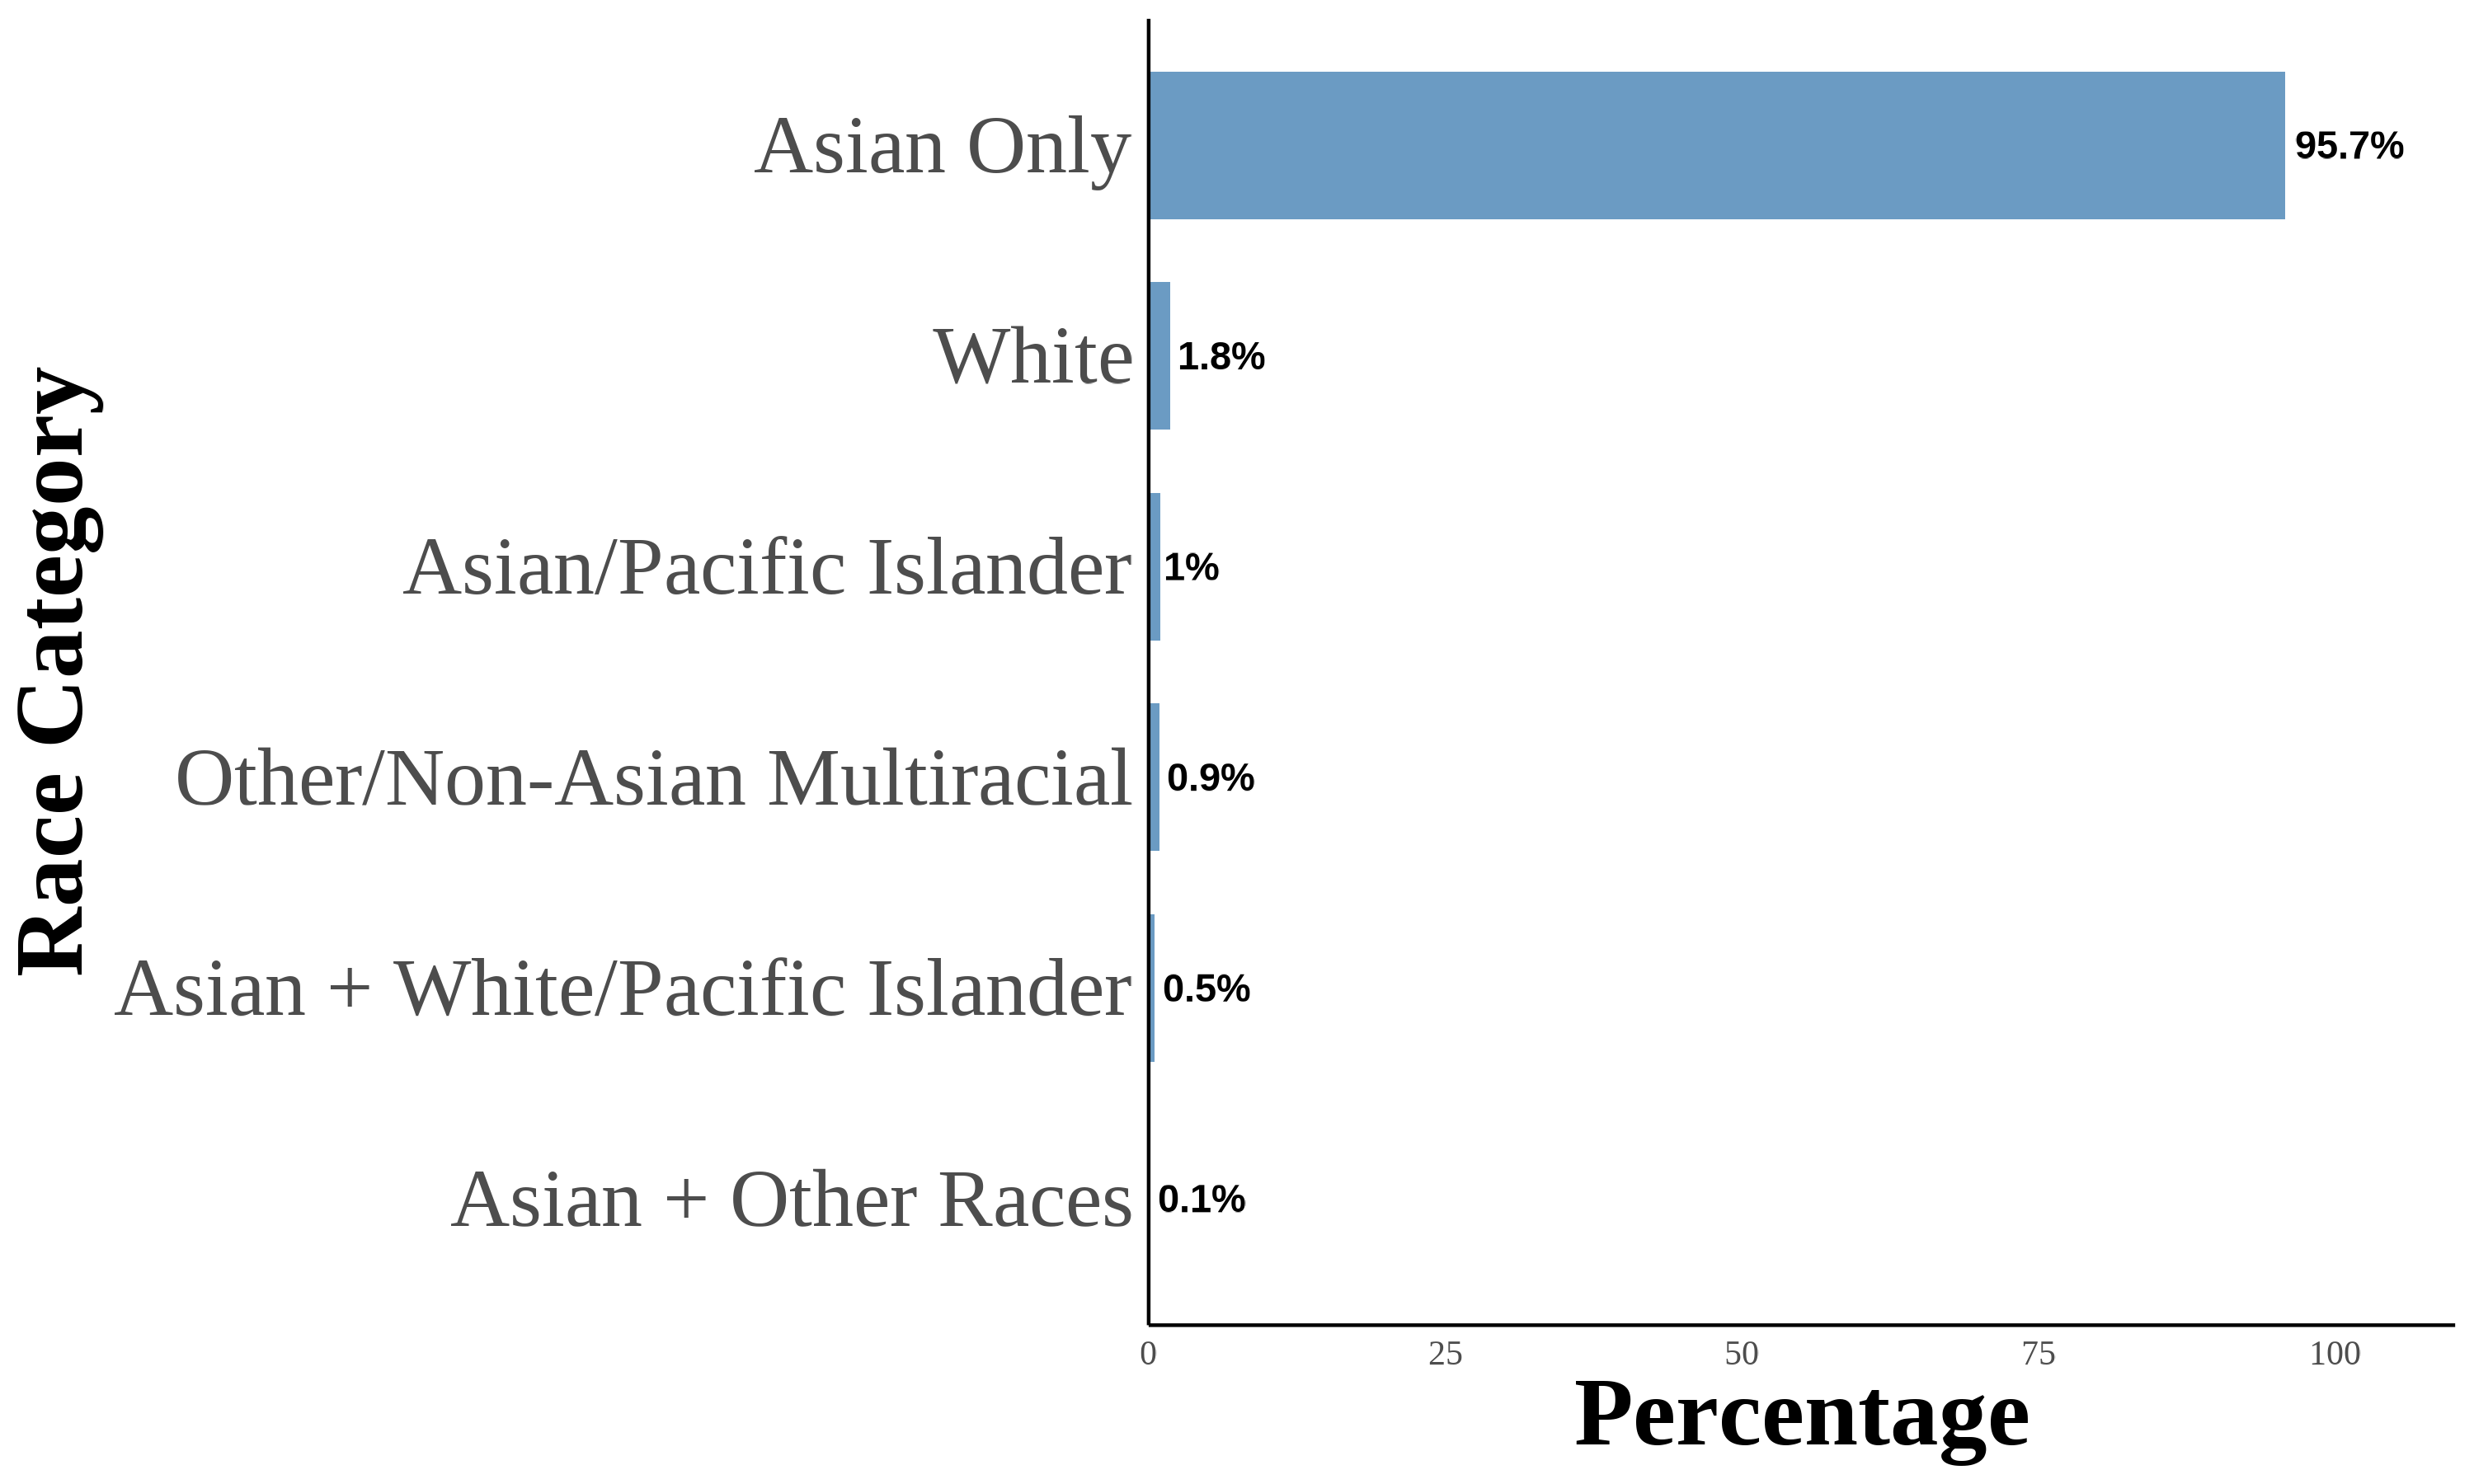
\includegraphics[width=1\linewidth]{histogram_asian_american_race_secondgen_AA.png}
\end{subfigure}

\vspace{1cm}

% Bottom row
\begin{subfigure}{.48\textwidth}
\caption{Second Generation: Asian Fathers-White Mothers}
\centering
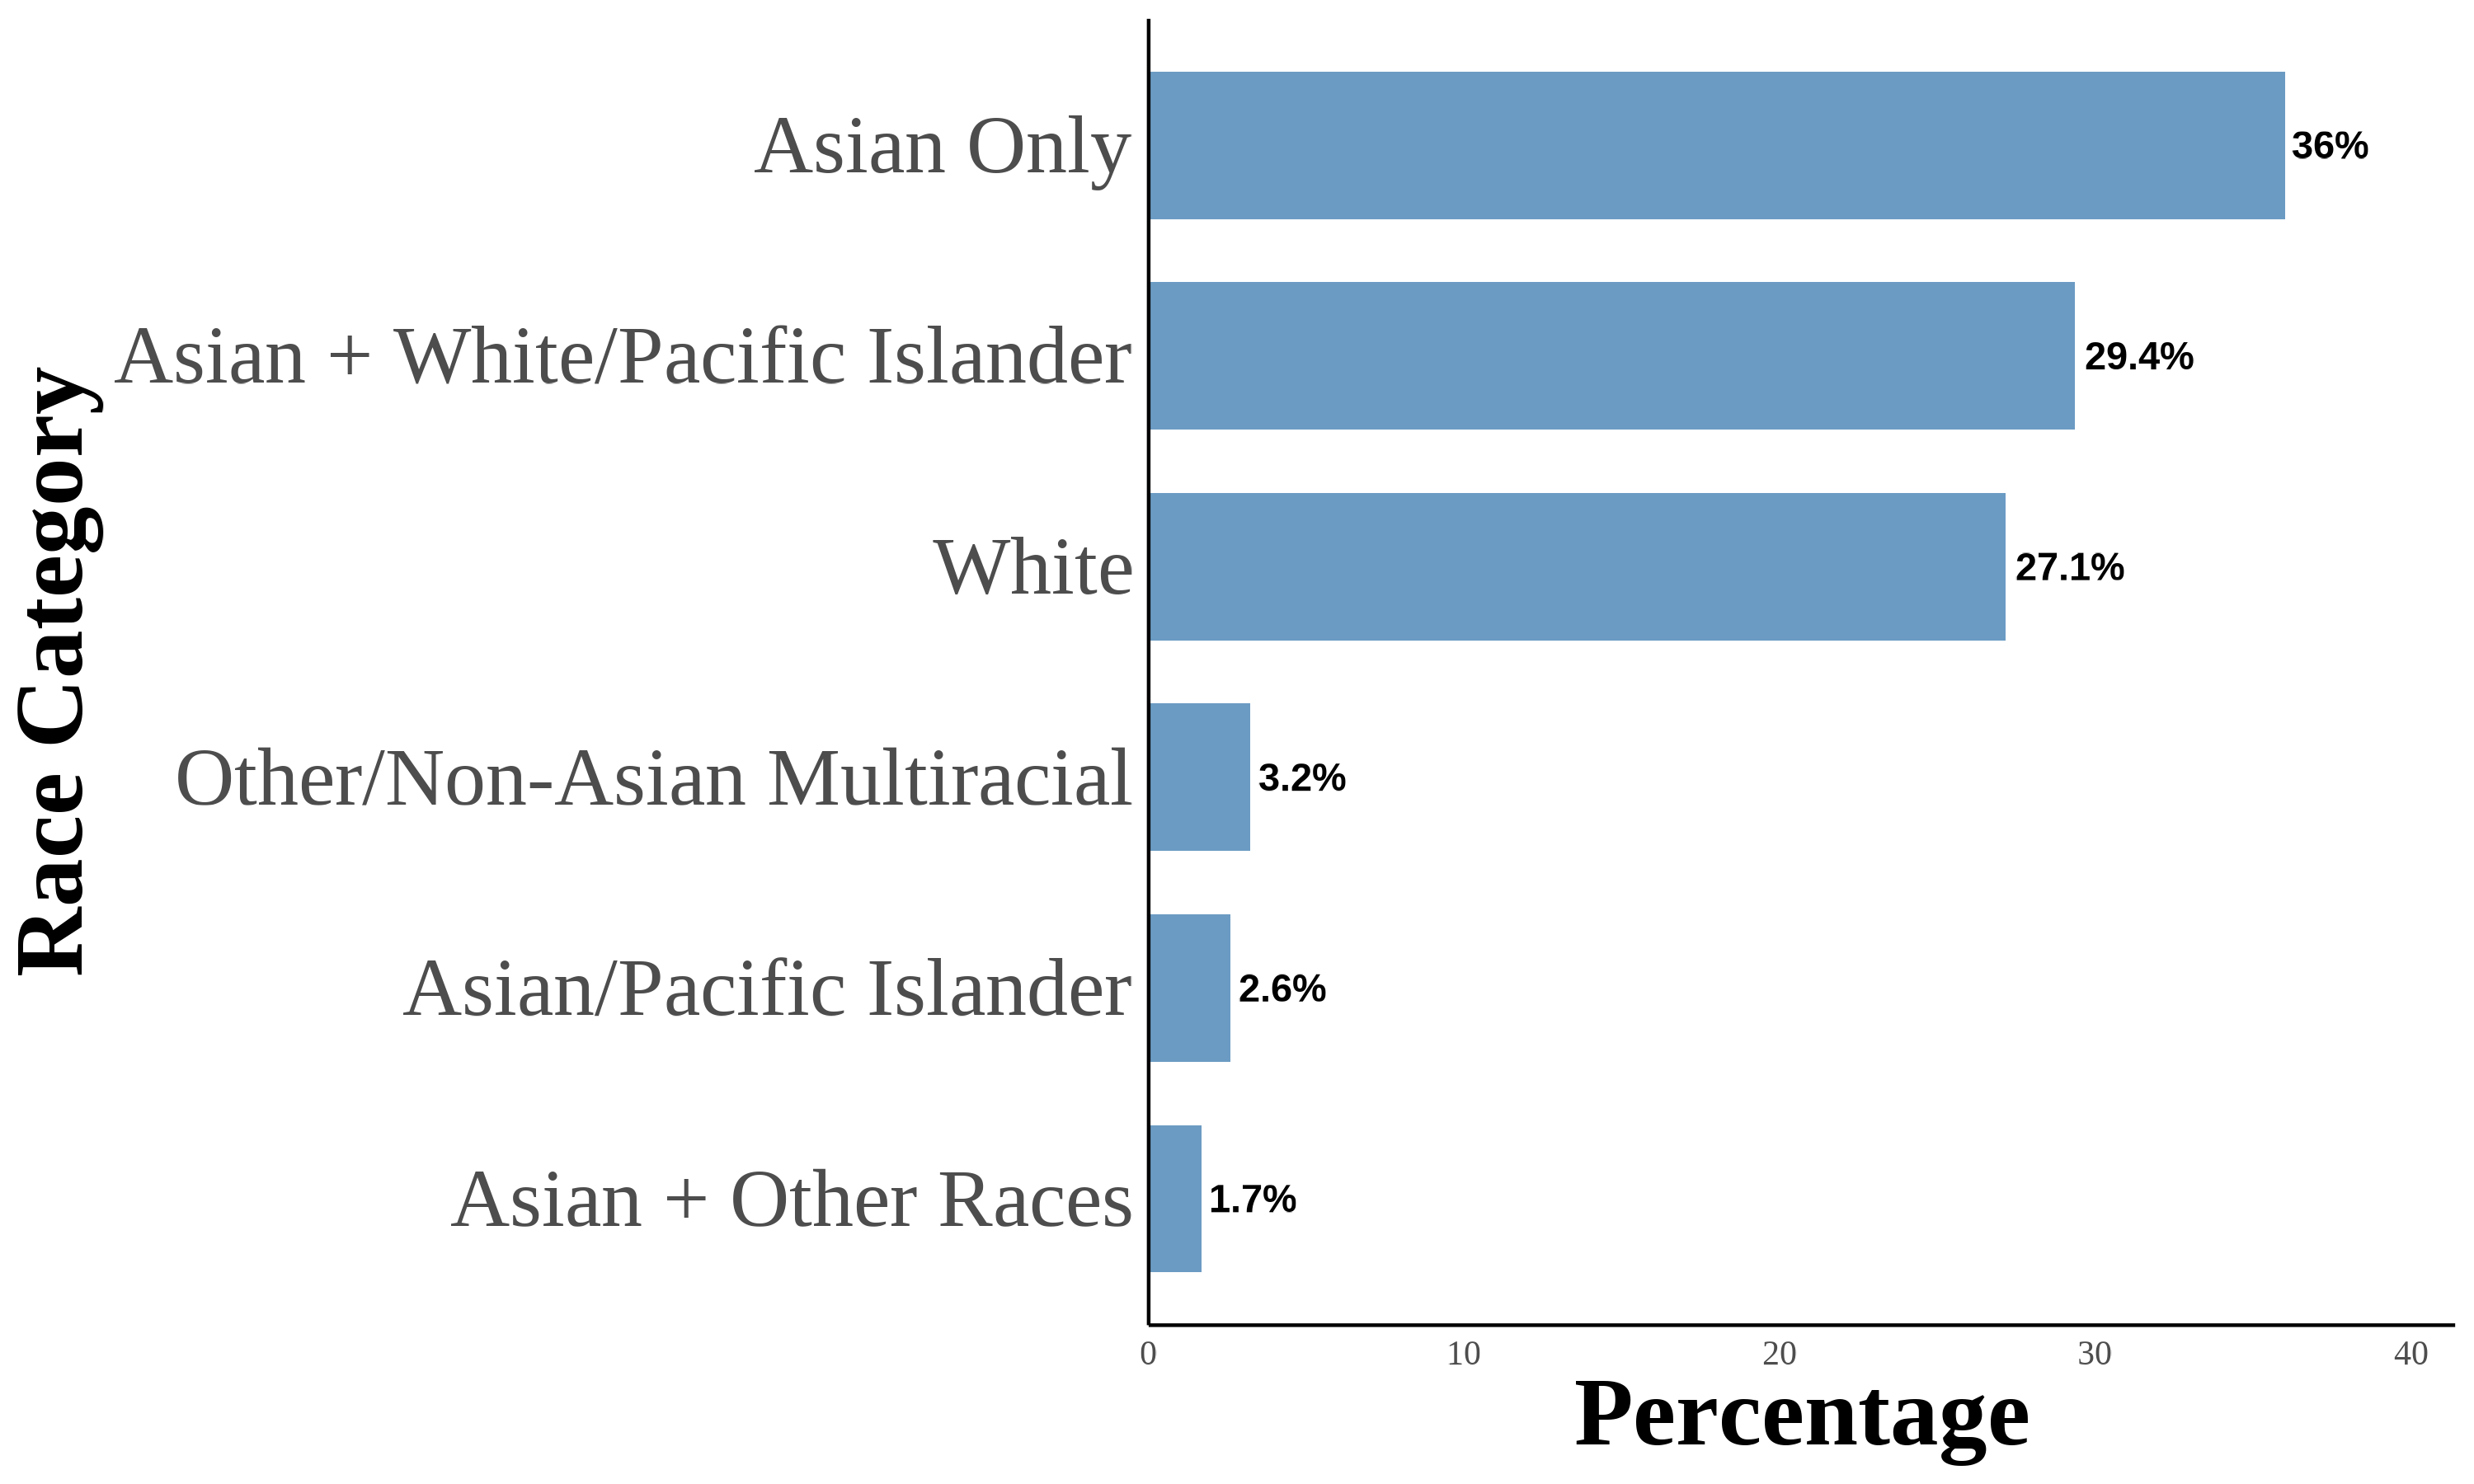
\includegraphics[width=1\linewidth]{histogram_asian_american_race_secondgen_AW.png}
\end{subfigure}
\hfill
\begin{subfigure}{.48\textwidth}
\caption{Second Generation: White Fathers-Asian Mothers}
\centering
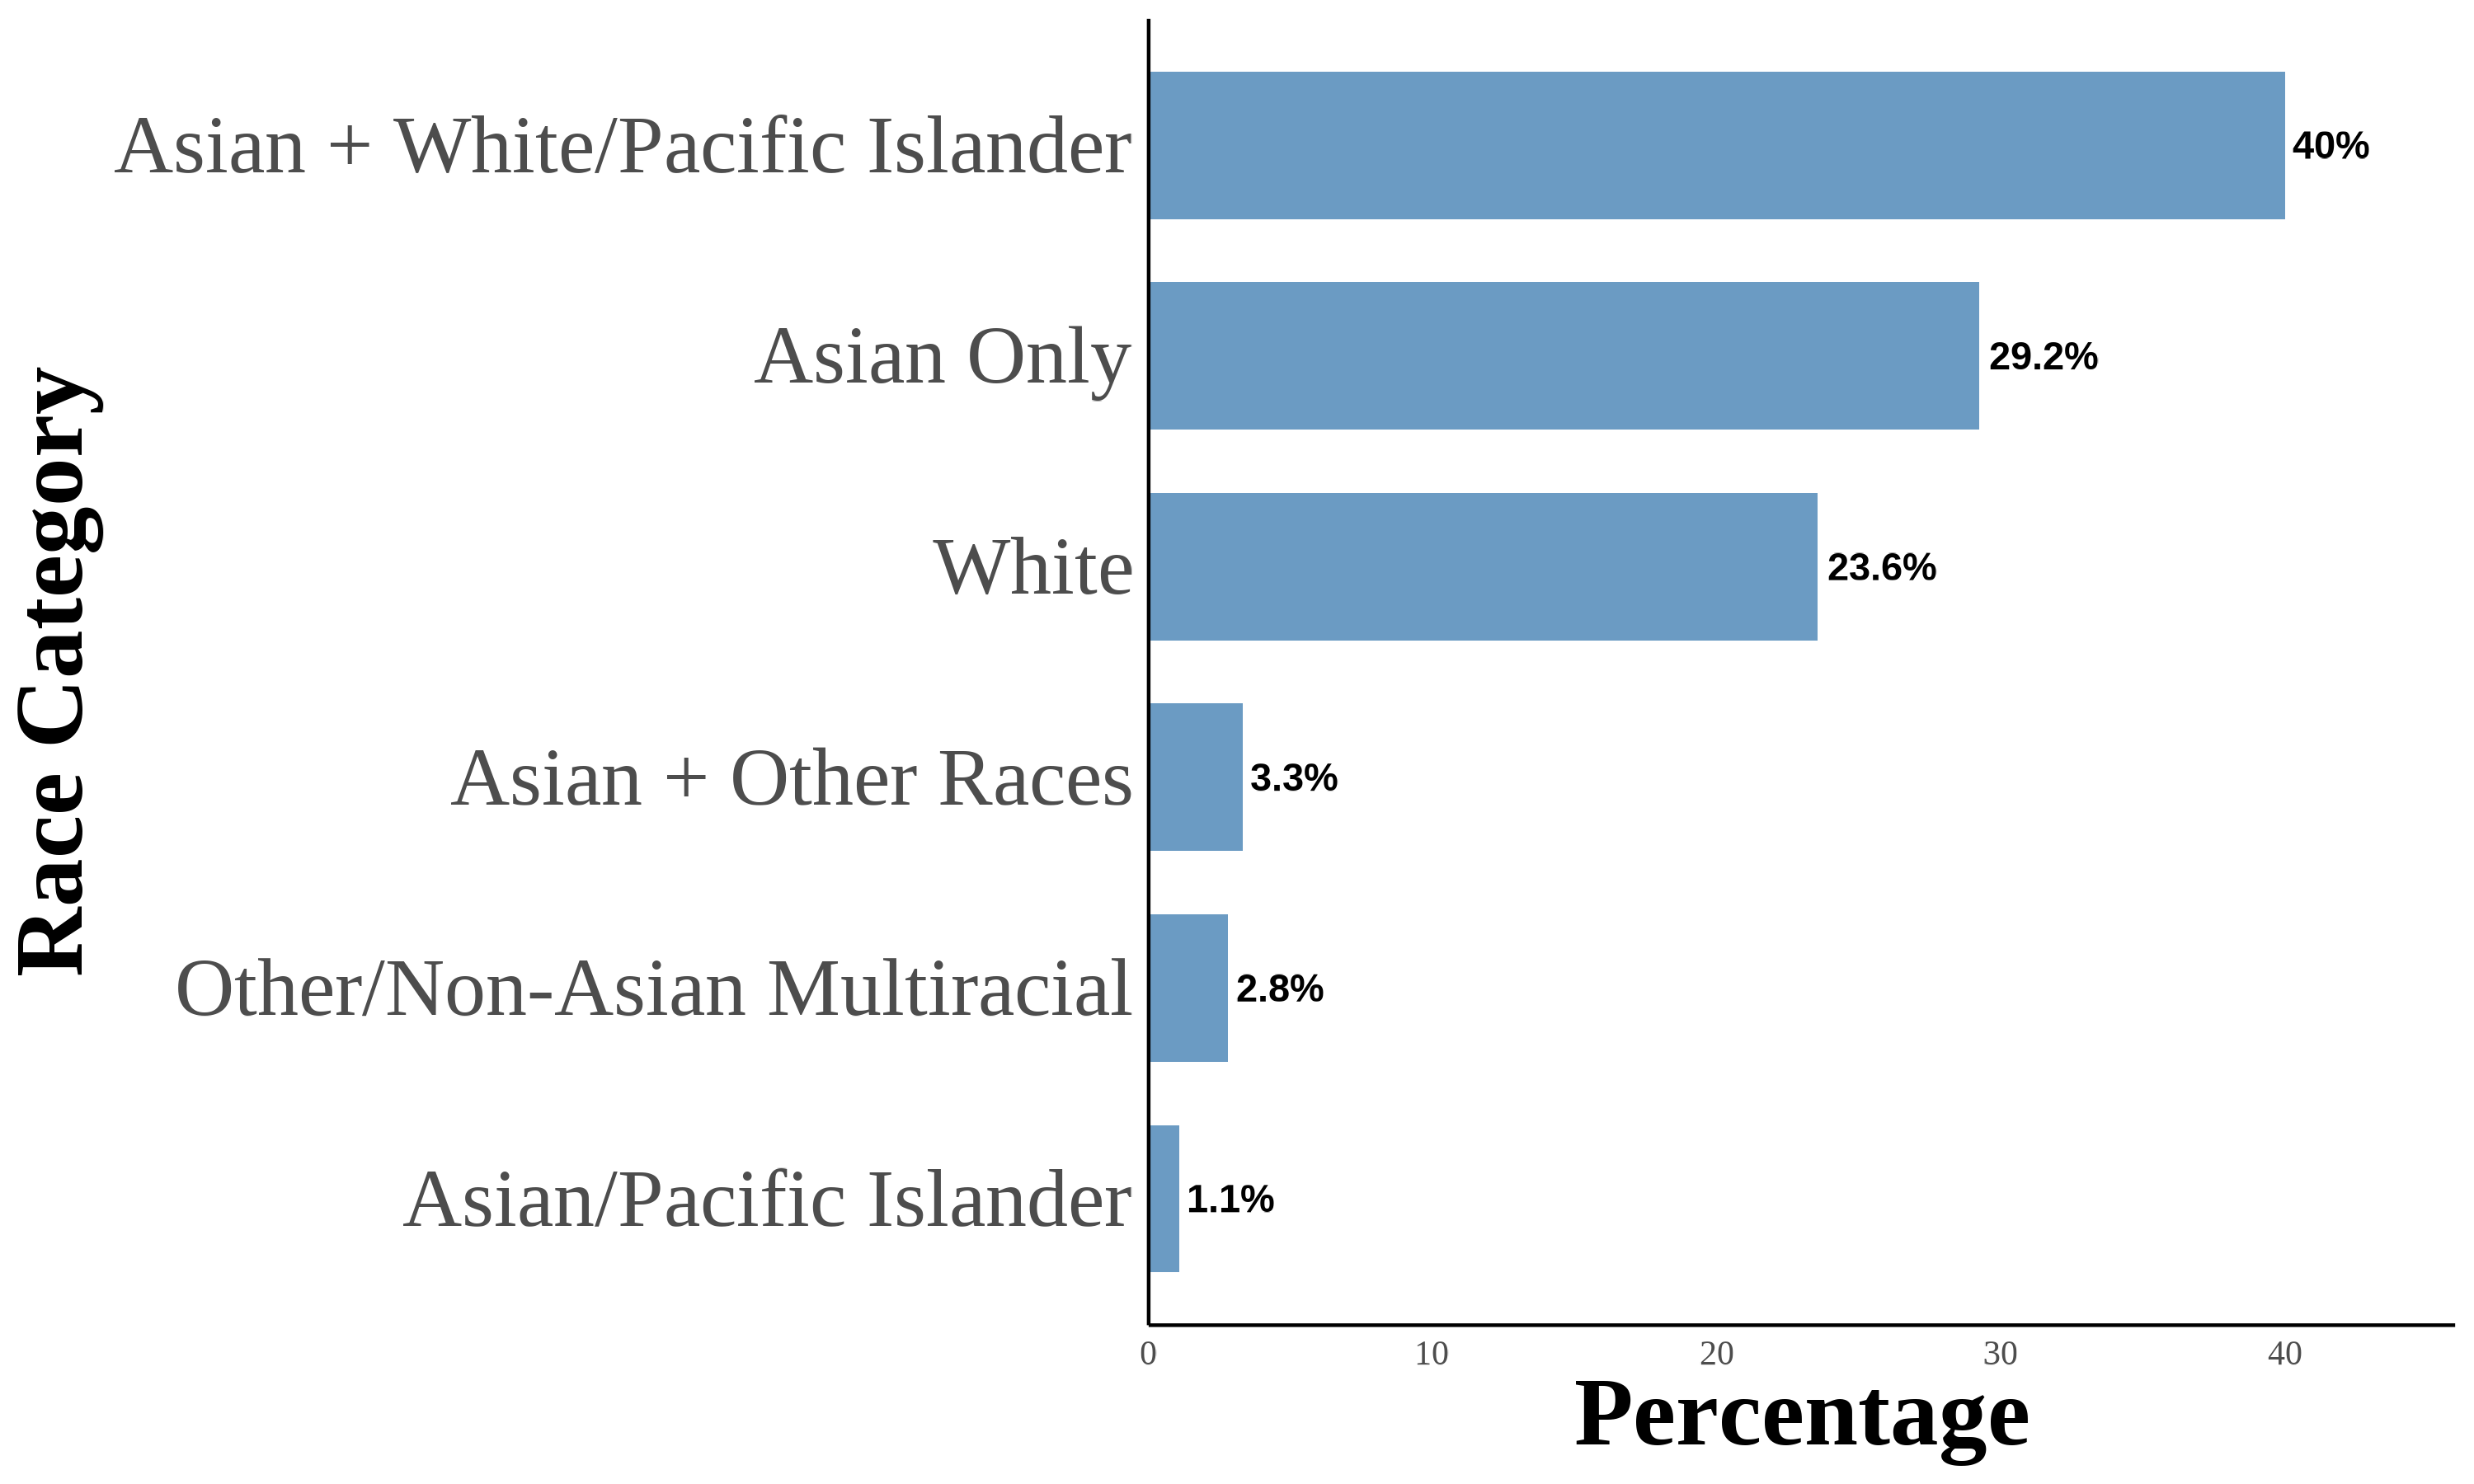
\includegraphics[width=1\linewidth]{histogram_asian_american_race_secondgen_WA.png}
\end{subfigure}

\caption*{\footnotesize{This figure shows the distribution of Asian racial identity among respondents. 
The data is aggregated from the 2004-2021 Current Population Survey (CPS). 
The sample includes second-generation objectively Asian Americans.
Following \textcite{antmanEthnicAttritionObserved2016,antmanEthnicAttritionAssimilation2020}, 
I utilize birthplace information for individuals, parents, and grandparents to create objective Asian ancestry indicators.
A second-generation Asian American is defined as a native-born individual with at least one parent born in an Asian country. 
The first panel is for second-generation Asian Americans. The second panel is for second-generation Asian Americans with both parents born in an Asian country. 
The third panel is for second-generation Asian Americans with an Asian father and a White mother. 
The fourth panel is for second-generation Asian Americans with a White father and an Asian mother.
}}
\end{figure}
\end{landscape}

\pagebreak
\newpage

\pagebreak
\newpage

\begin{landscape}
\begin{figure}[!htb]
\centering
\caption{Asian Racial Identity: Third Generation}
\label{fig:histogram-thirdgen}

% Top row - 3 graphs
\begin{subfigure}{.32\textwidth}
\caption{All Third Generation}
\centering
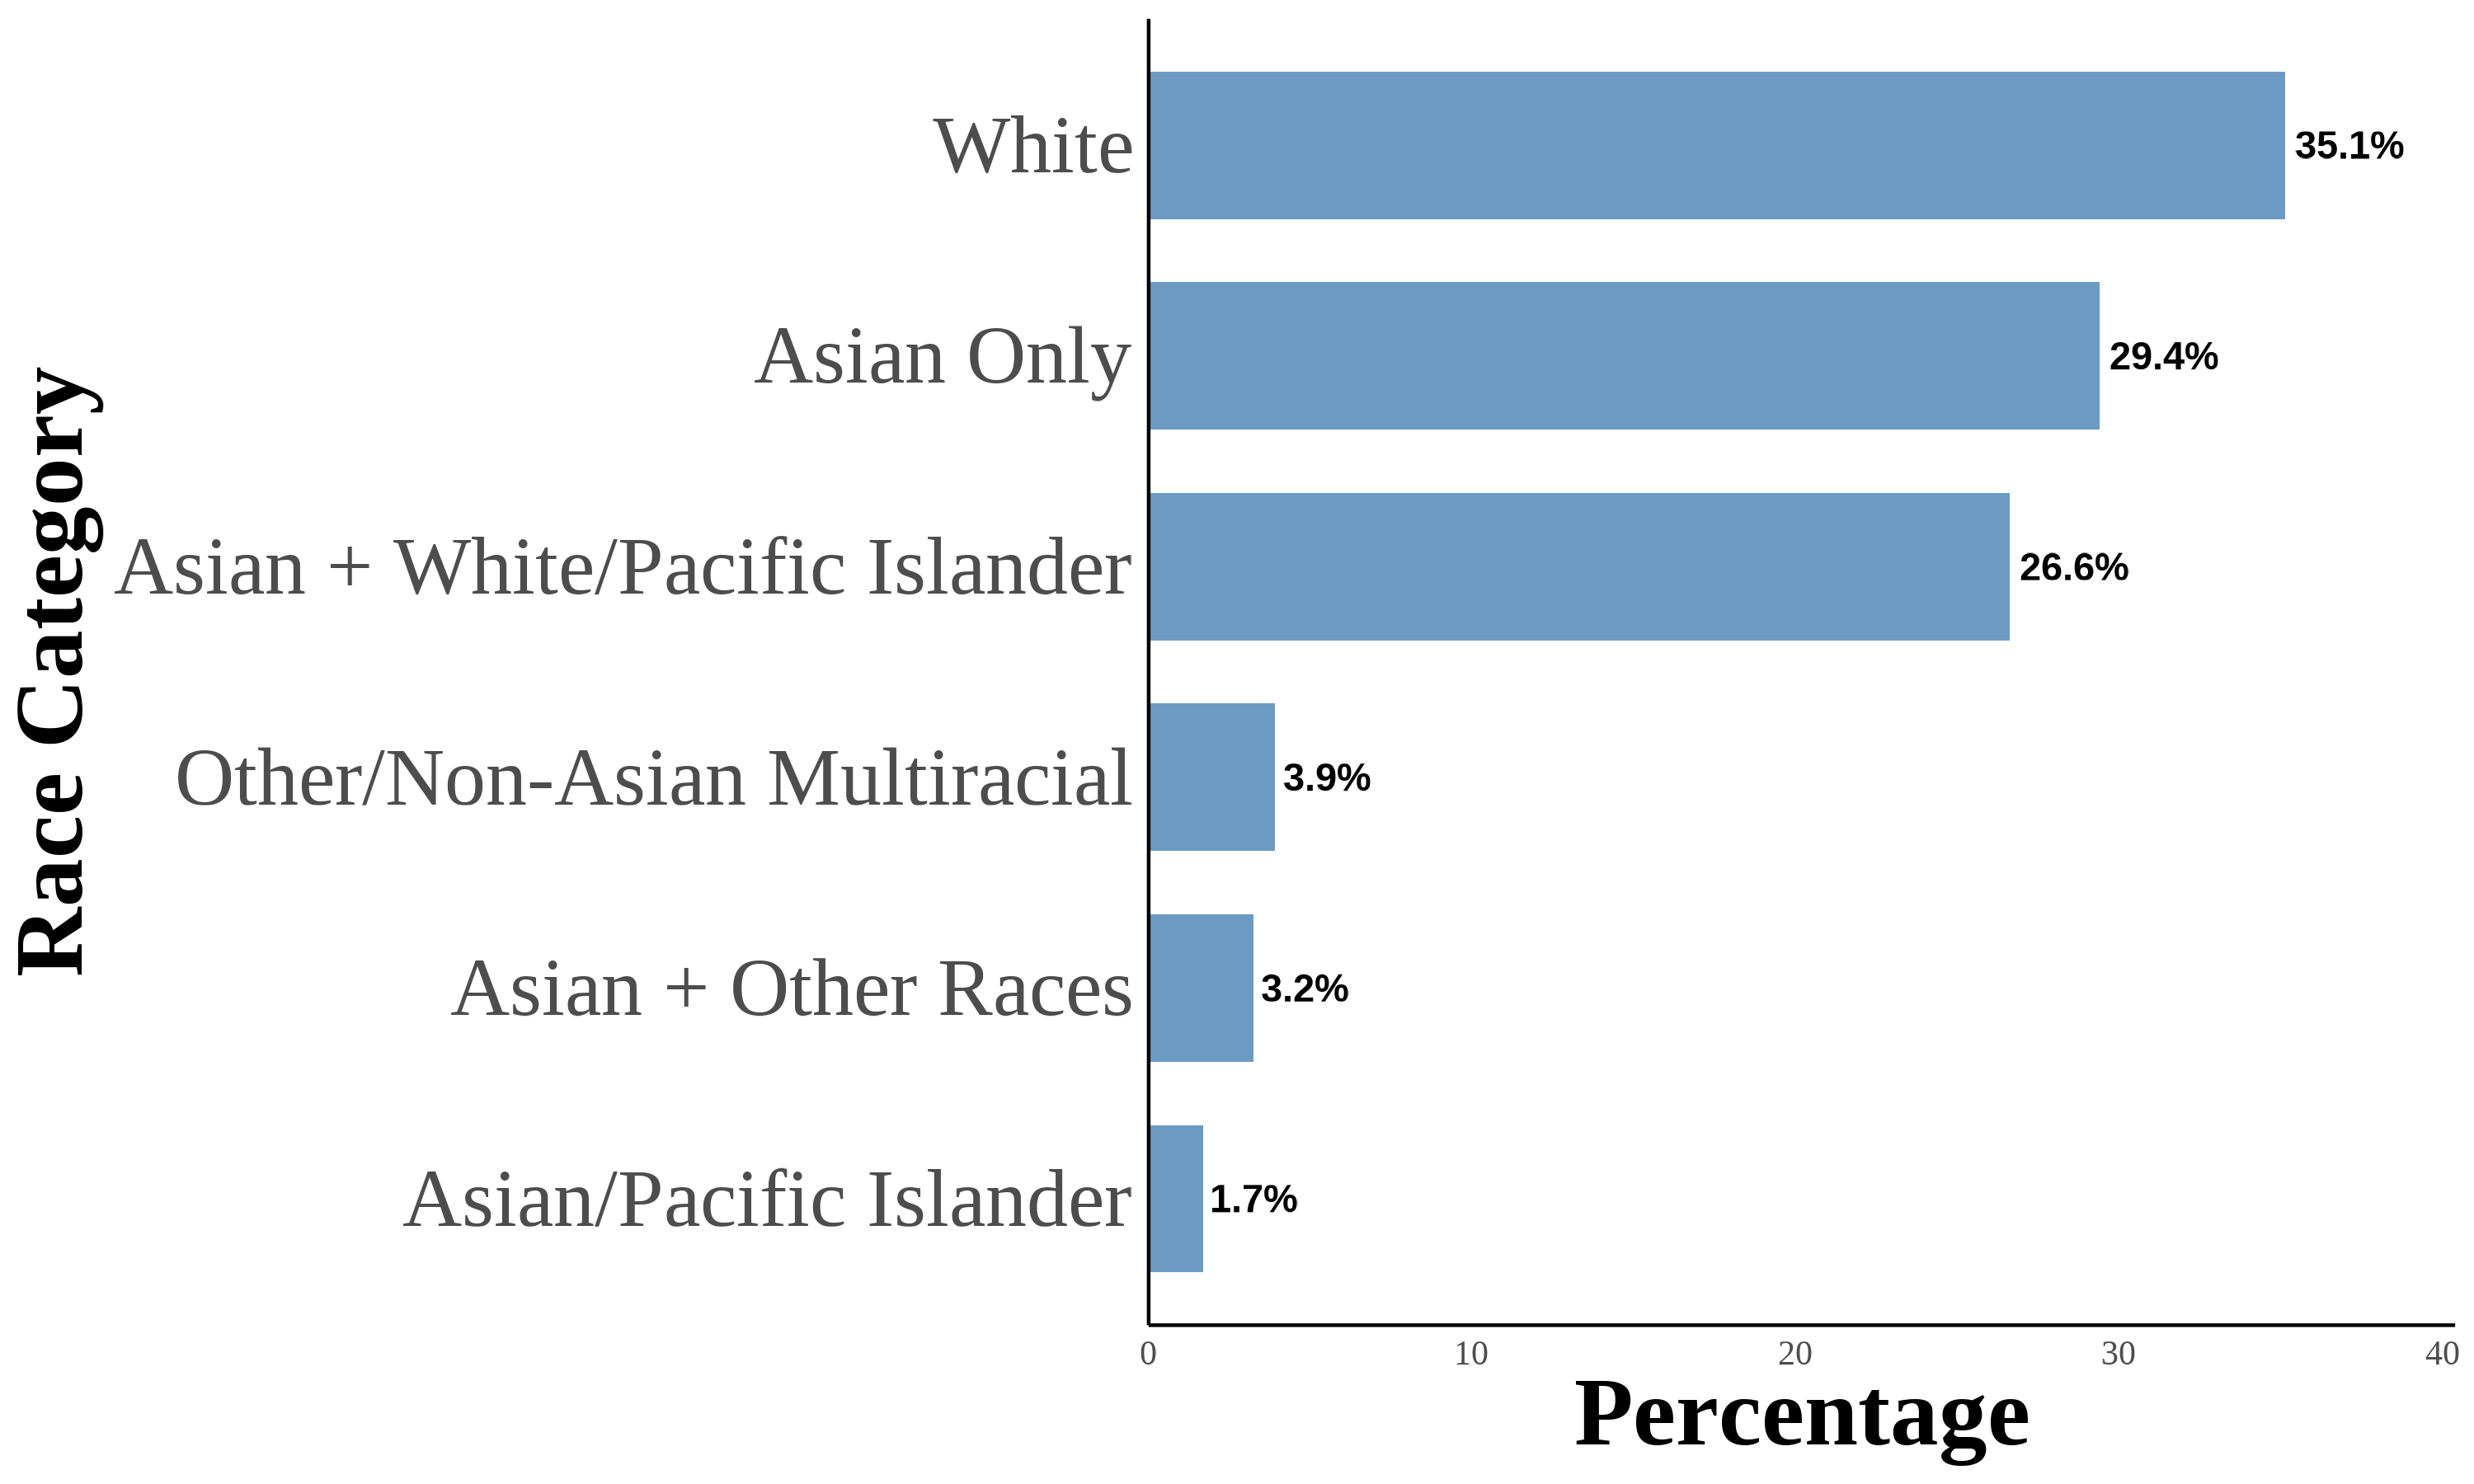
\includegraphics[width=1\linewidth]{histogram_asian_american_race_thirdgen.png}
\end{subfigure}
\hfill
\begin{subfigure}{.32\textwidth}
\caption{Third Generation: One Asian Grandparent}
\centering
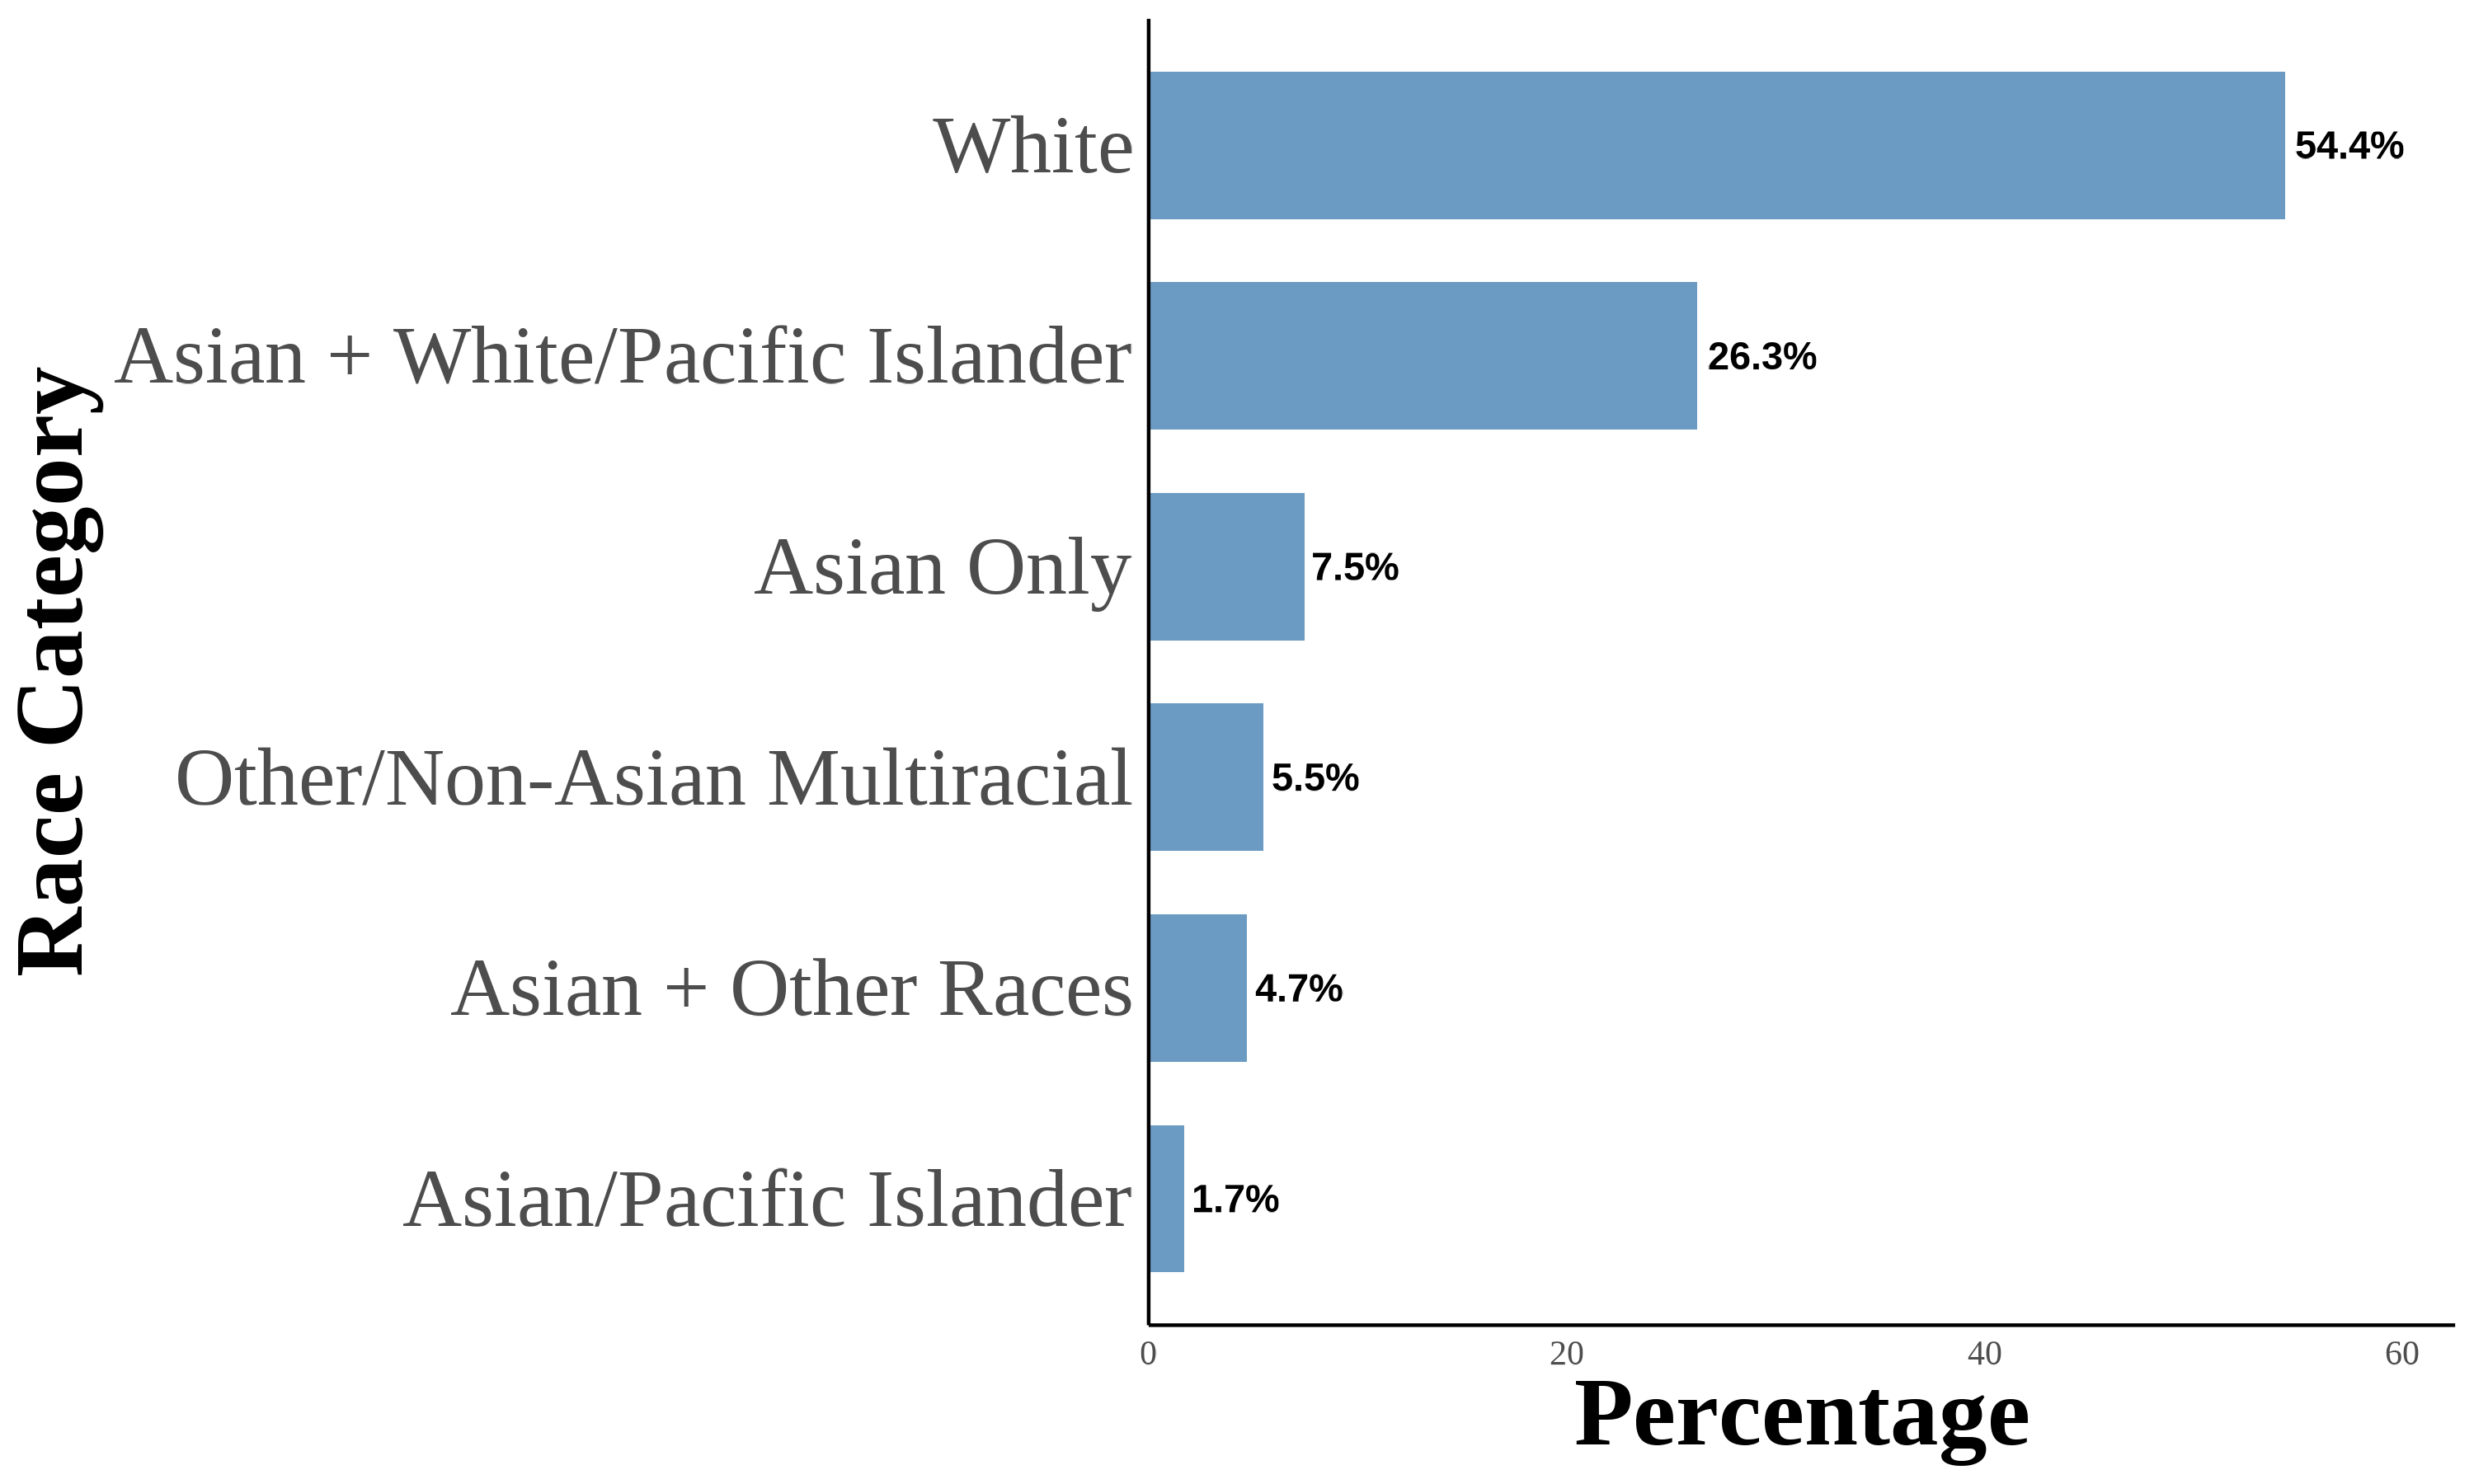
\includegraphics[width=1\linewidth]{histogram_asian_american_race_thirdgen_oneasiangran.png}
\end{subfigure}
\hfill
\begin{subfigure}{.32\textwidth}
\caption{Third Generation: Two Asian Grandparents}
\centering
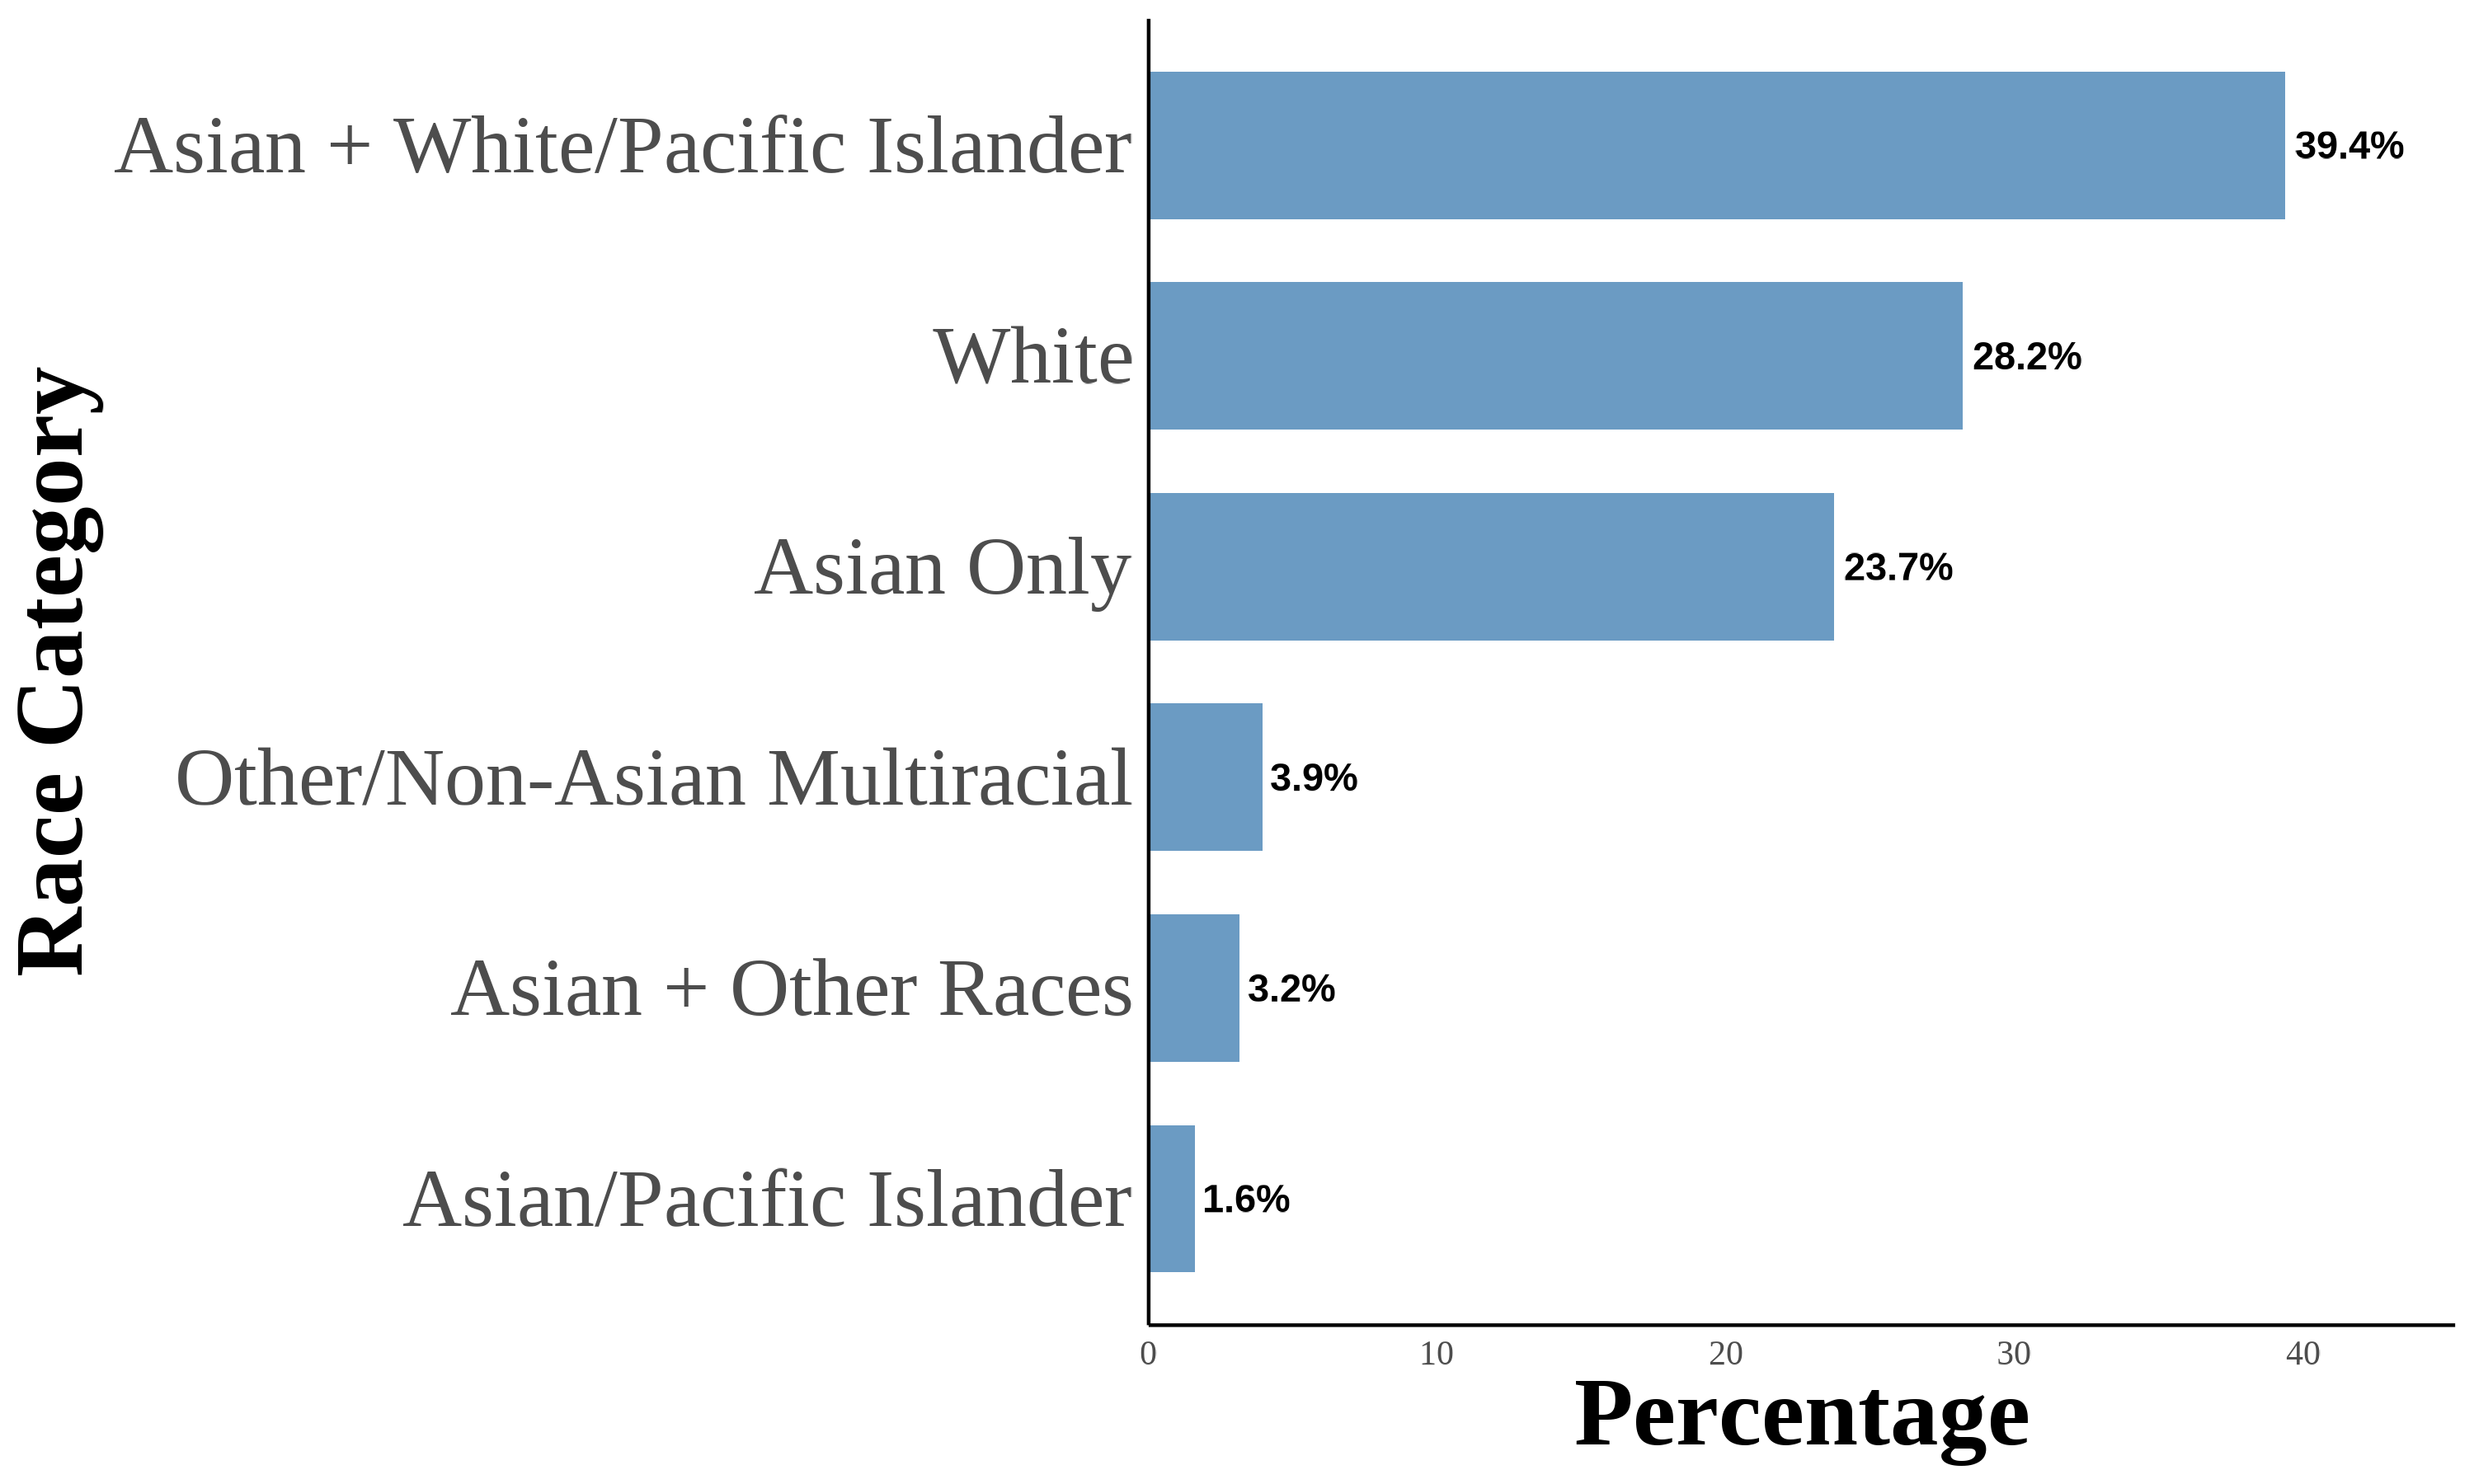
\includegraphics[width=1\linewidth]{histogram_asian_american_race_thirdgen_twoasiangran.png}
\end{subfigure}

\vspace{1cm}

% Bottom row - 2 graphs centered with more space
\hspace*{\fill}
\begin{subfigure}{.4\textwidth}
\caption{Third Generation: Three Asian Grandparents}
\centering
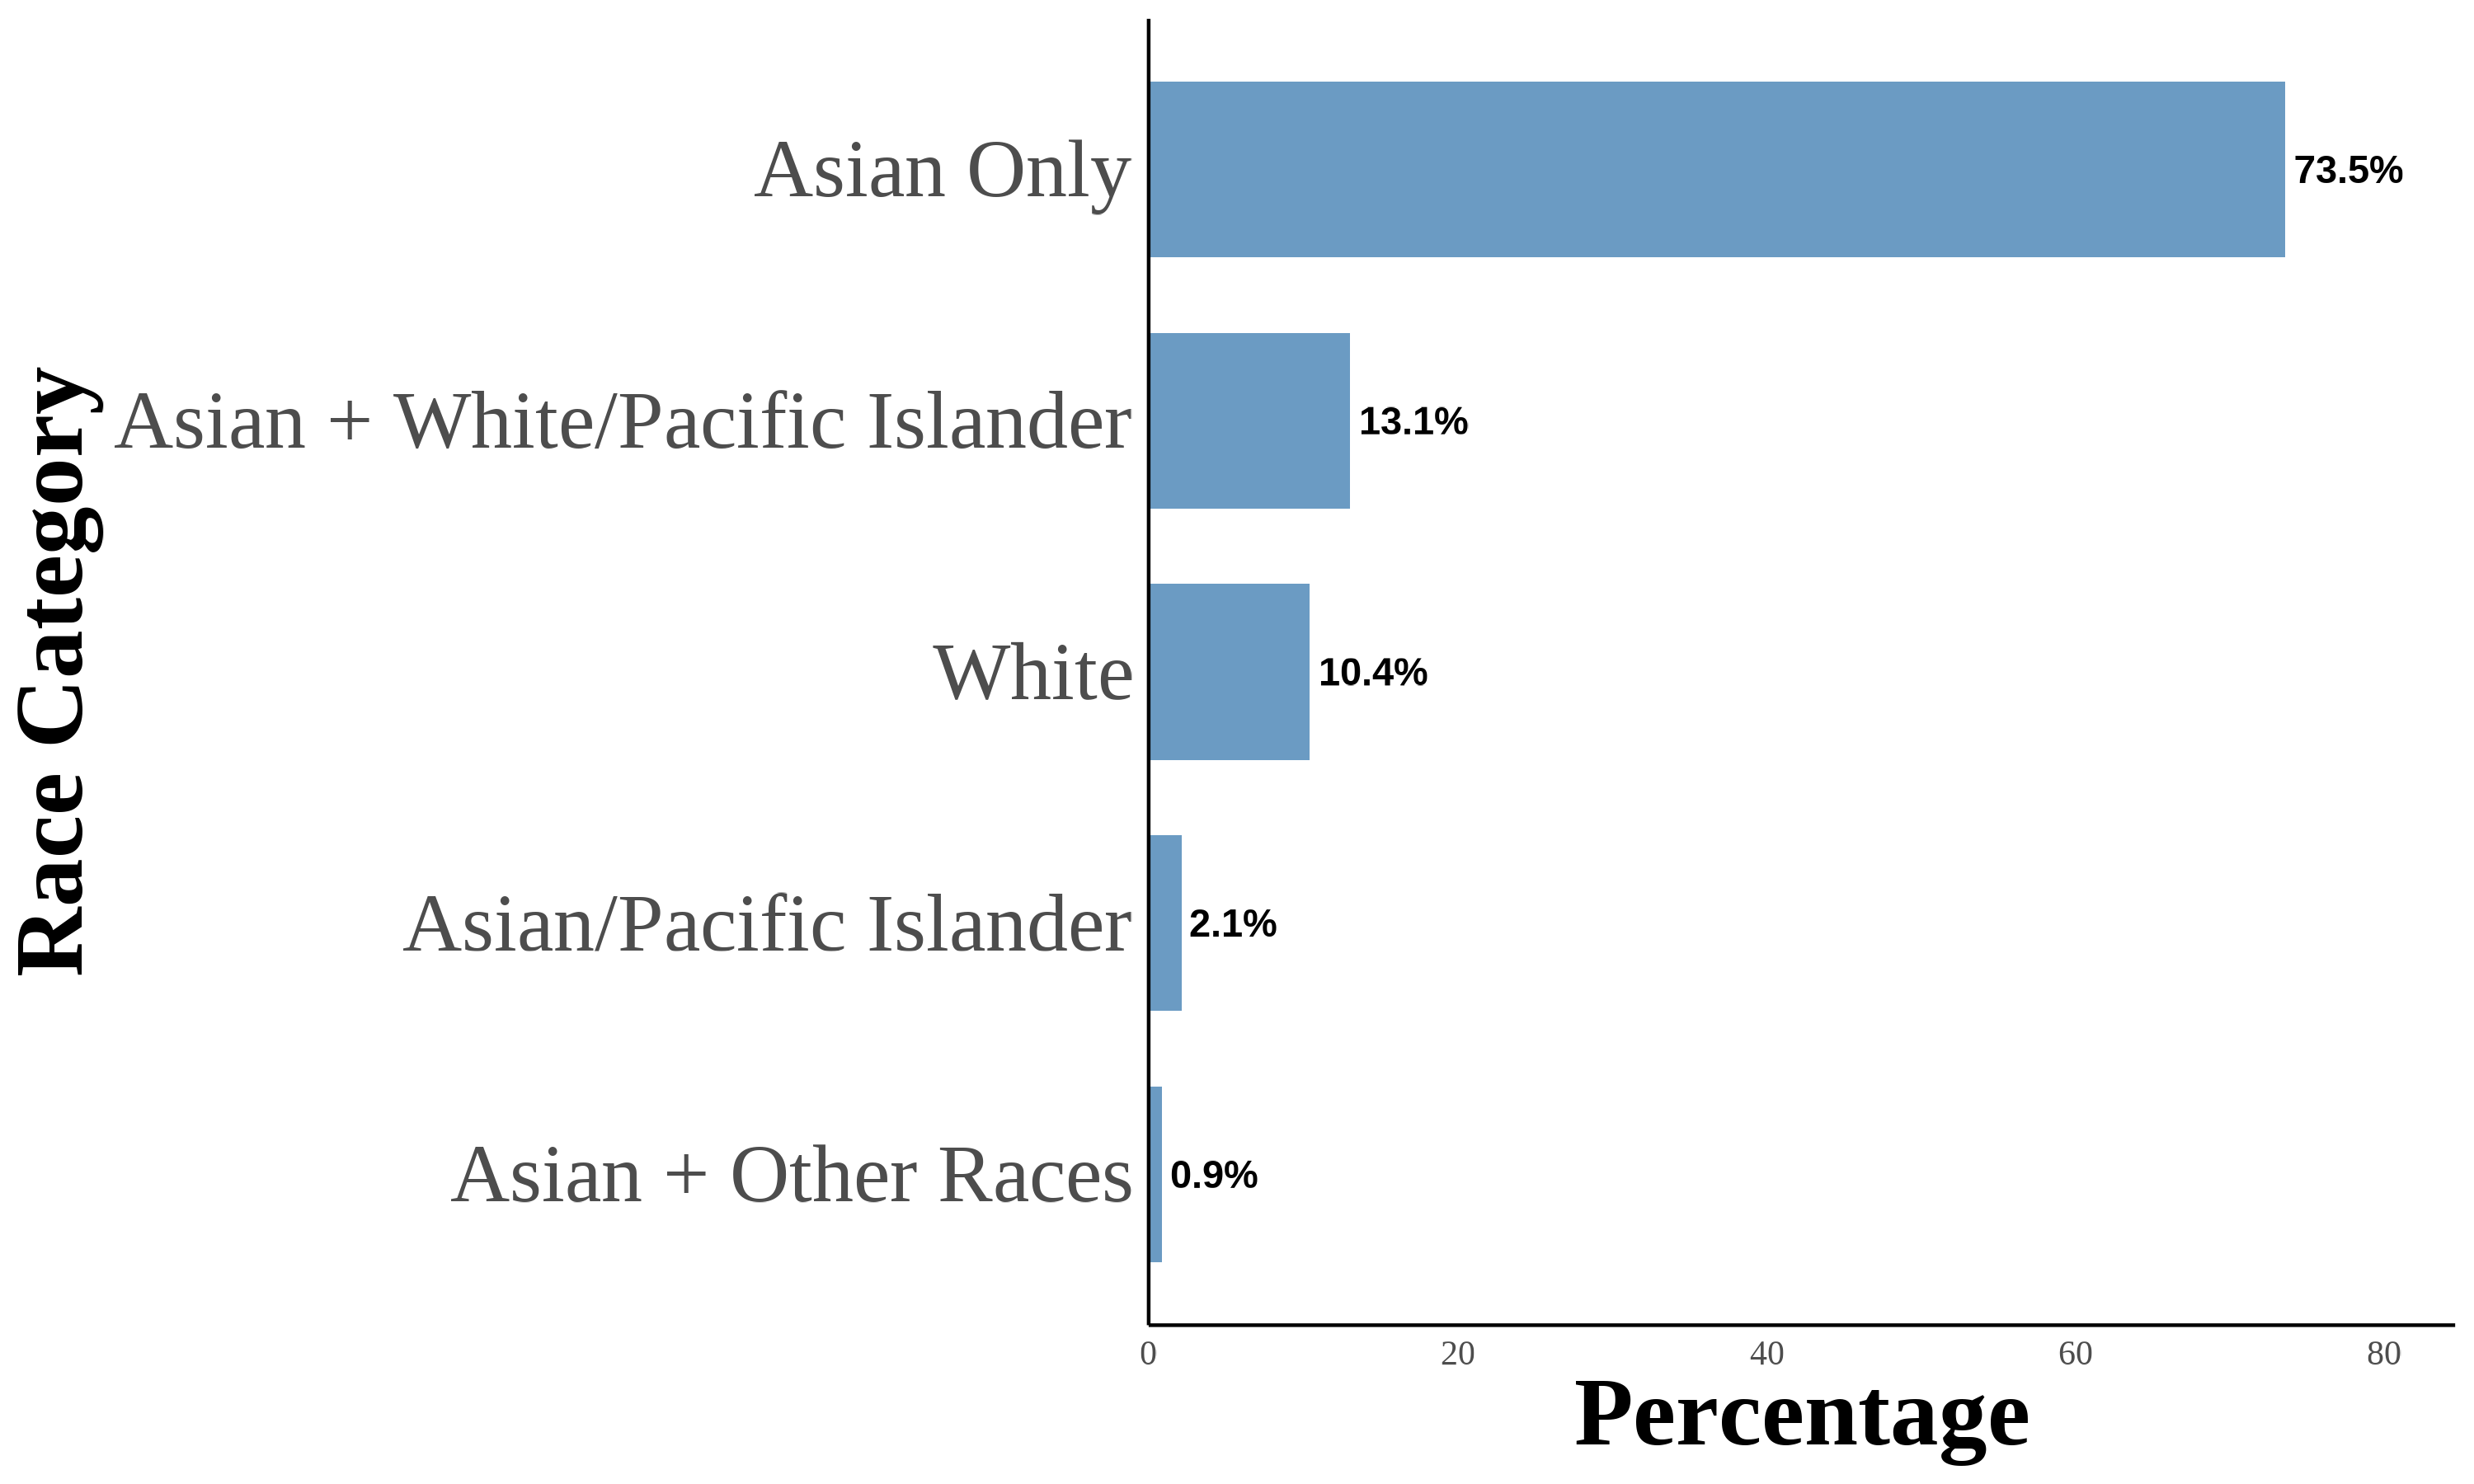
\includegraphics[width=1\linewidth]{histogram_asian_american_race_thirdgen_threeasiangran.png}
\end{subfigure}
\hfill
\begin{subfigure}{.4\textwidth}
\caption{Third Generation: Four Asian Grandparents}
\centering
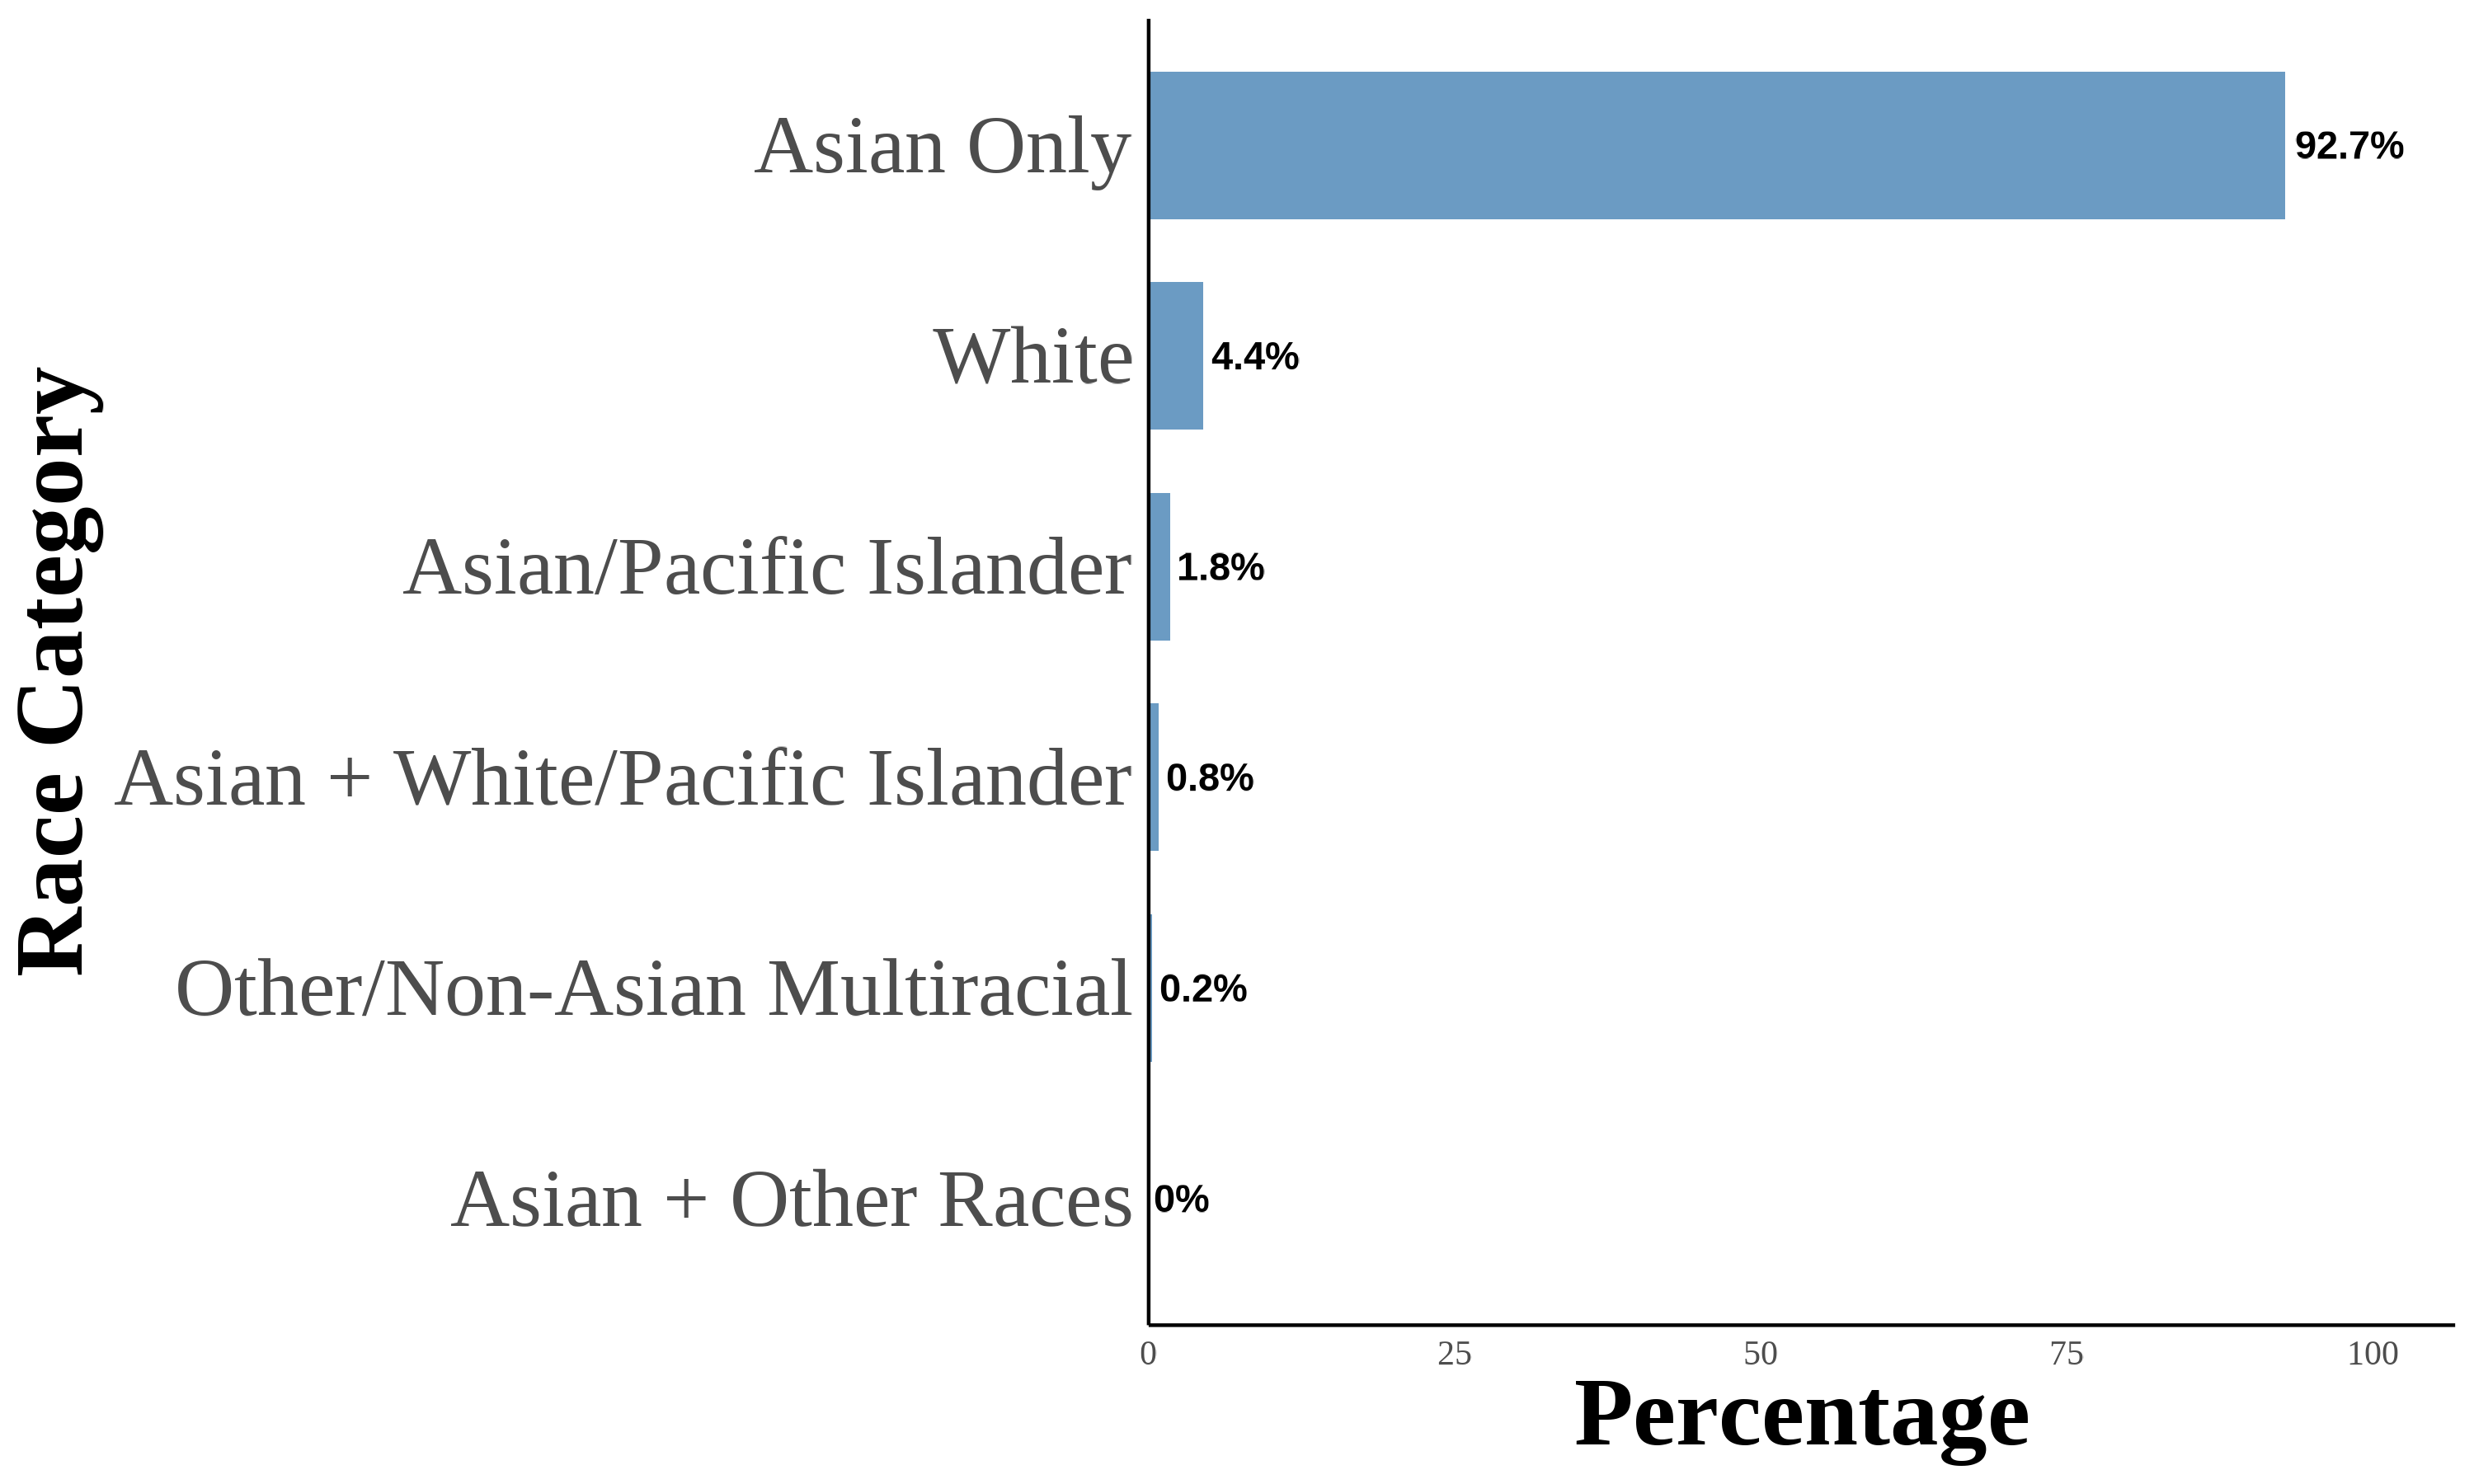
\includegraphics[width=1\linewidth]{histogram_asian_american_race_thirdgen_fourasiangran.png}
\end{subfigure}
\hspace*{\fill}

\caption*{\footnotesize{This figure shows the distribution of Asian racial identity among respondents. 
The data is aggregated from the 2004-2021 Current Population Survey (CPS). 
The sample includes second-generation objectively Asian Americans.
Following \textcite{antmanEthnicAttritionObserved2016,antmanEthnicAttritionAssimilation2020}, 
I utilize birthplace information for individuals, parents, and grandparents to create objective Asian ancestry indicators.
A third-generation Asian American is defined as a native-born individual with native-born parents and at least one grandparent born in an Asian country. 
The first panel is for third-generation Asian Americans. The second panel is for third-generation Asian Americans with one grandparent born in an Asian country. 
The third panel is for third-generation Asian Americans with two grandparents born in an Asian country. 
The fourth panel is for third-generation Asian Americans with three grandparents born in an Asian country.
The fifth panel is for third-generation Asian Americans with four grandparents born in an Asian country.
}}
\end{figure}
\end{landscape}

\pagebreak
\newpage

\begin{center}
\begin{figure}[!htb]
\centering
\caption{Relationship Between Self-Reported Asian Identity and Bias: By Generation}
\label{plot01-regression-gen}
%First graph
\begin{subfigure}{.48\textwidth}
\caption{All Generations}
\centering
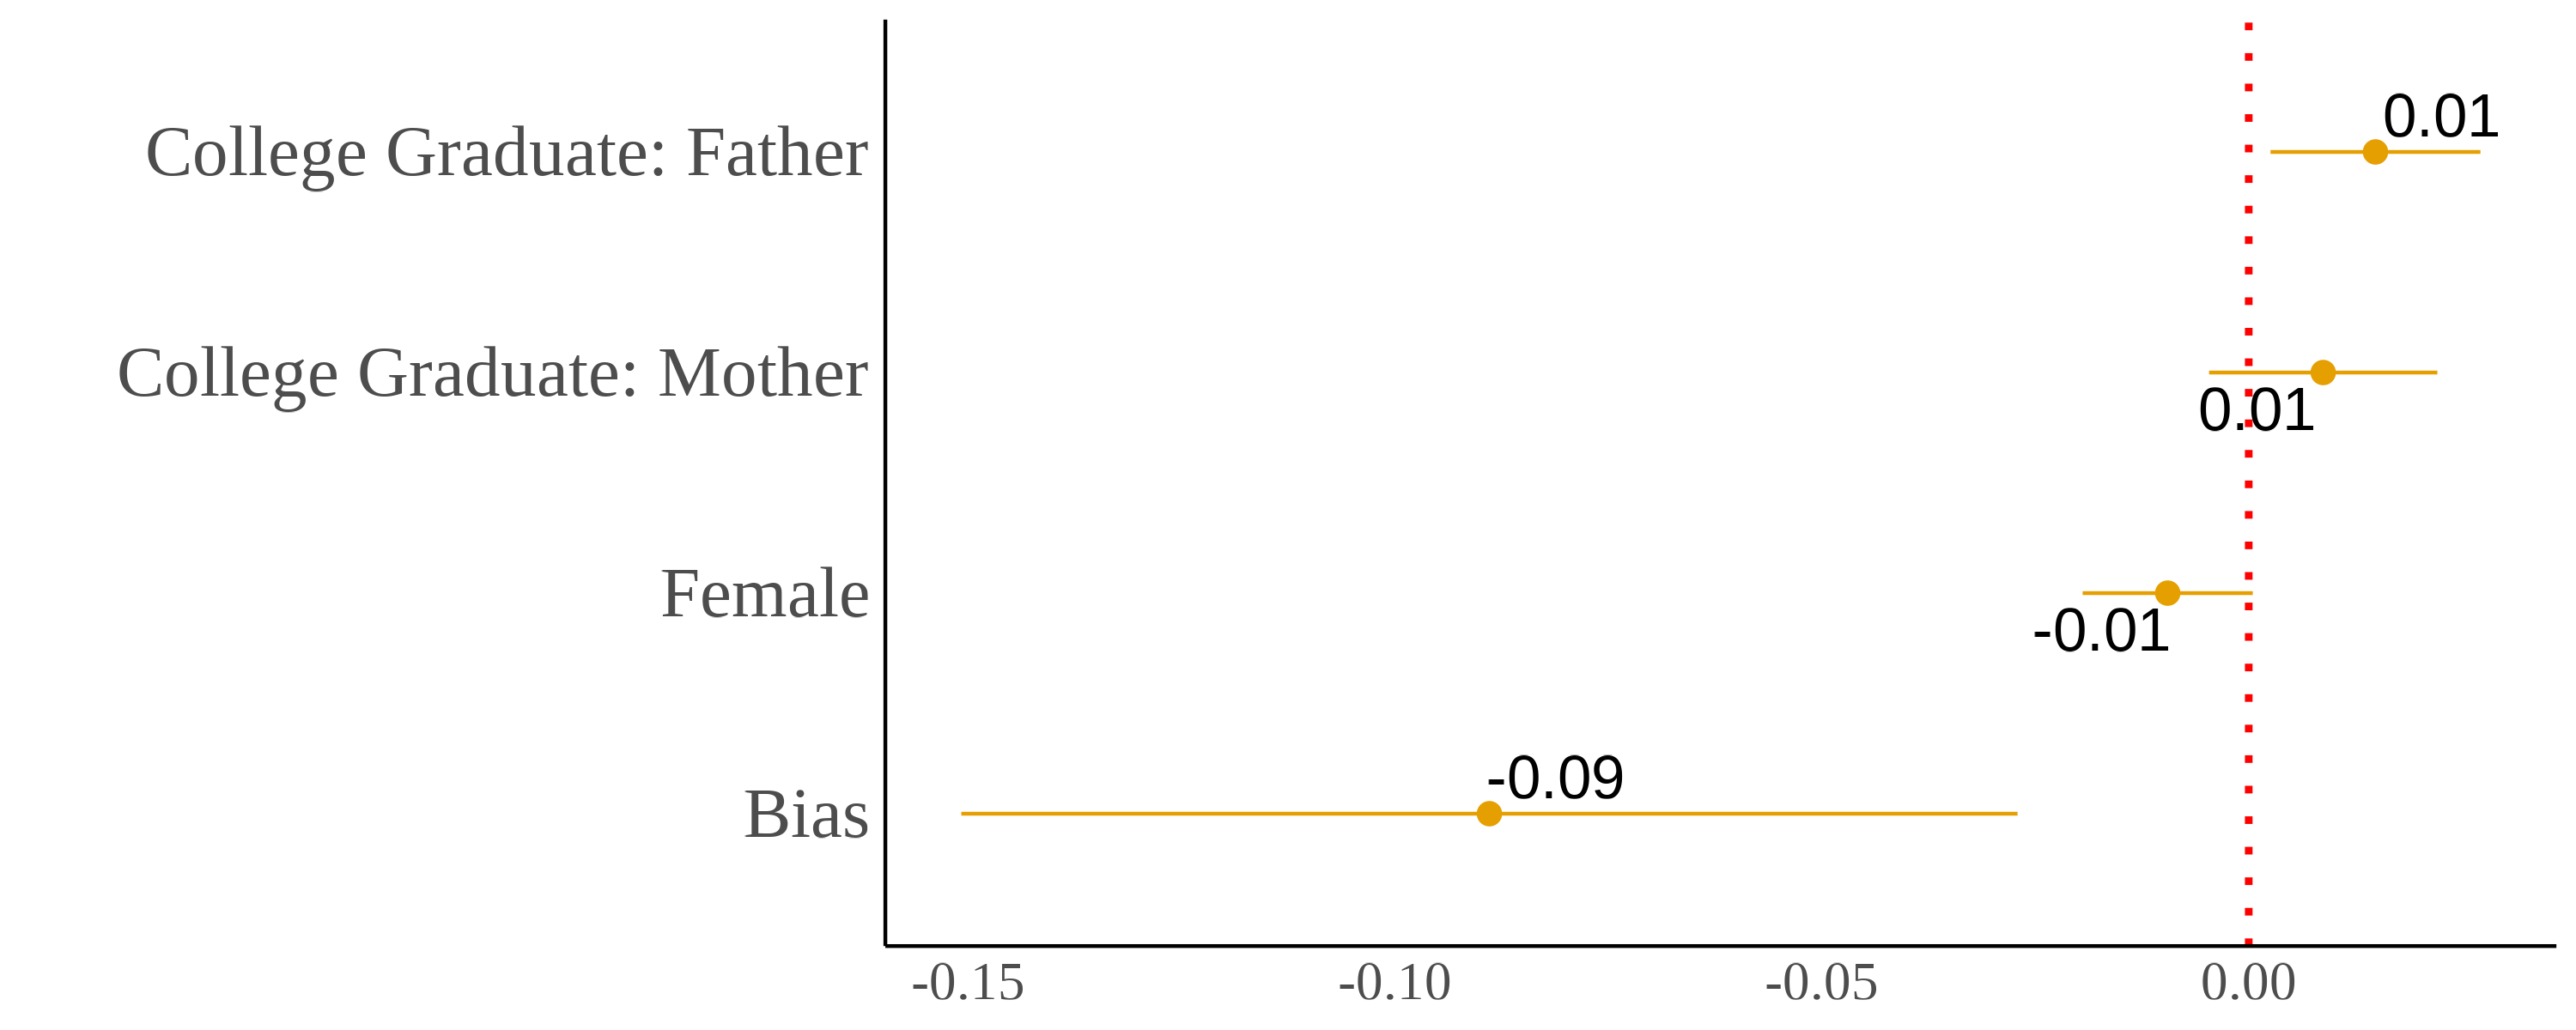
\includegraphics[width=.9\linewidth]{skin-iat-regression-all-gens.png}
\end{subfigure}
\centering
%Second graph
\begin{subfigure}{.48\textwidth}
\caption{First-Generation}
\centering
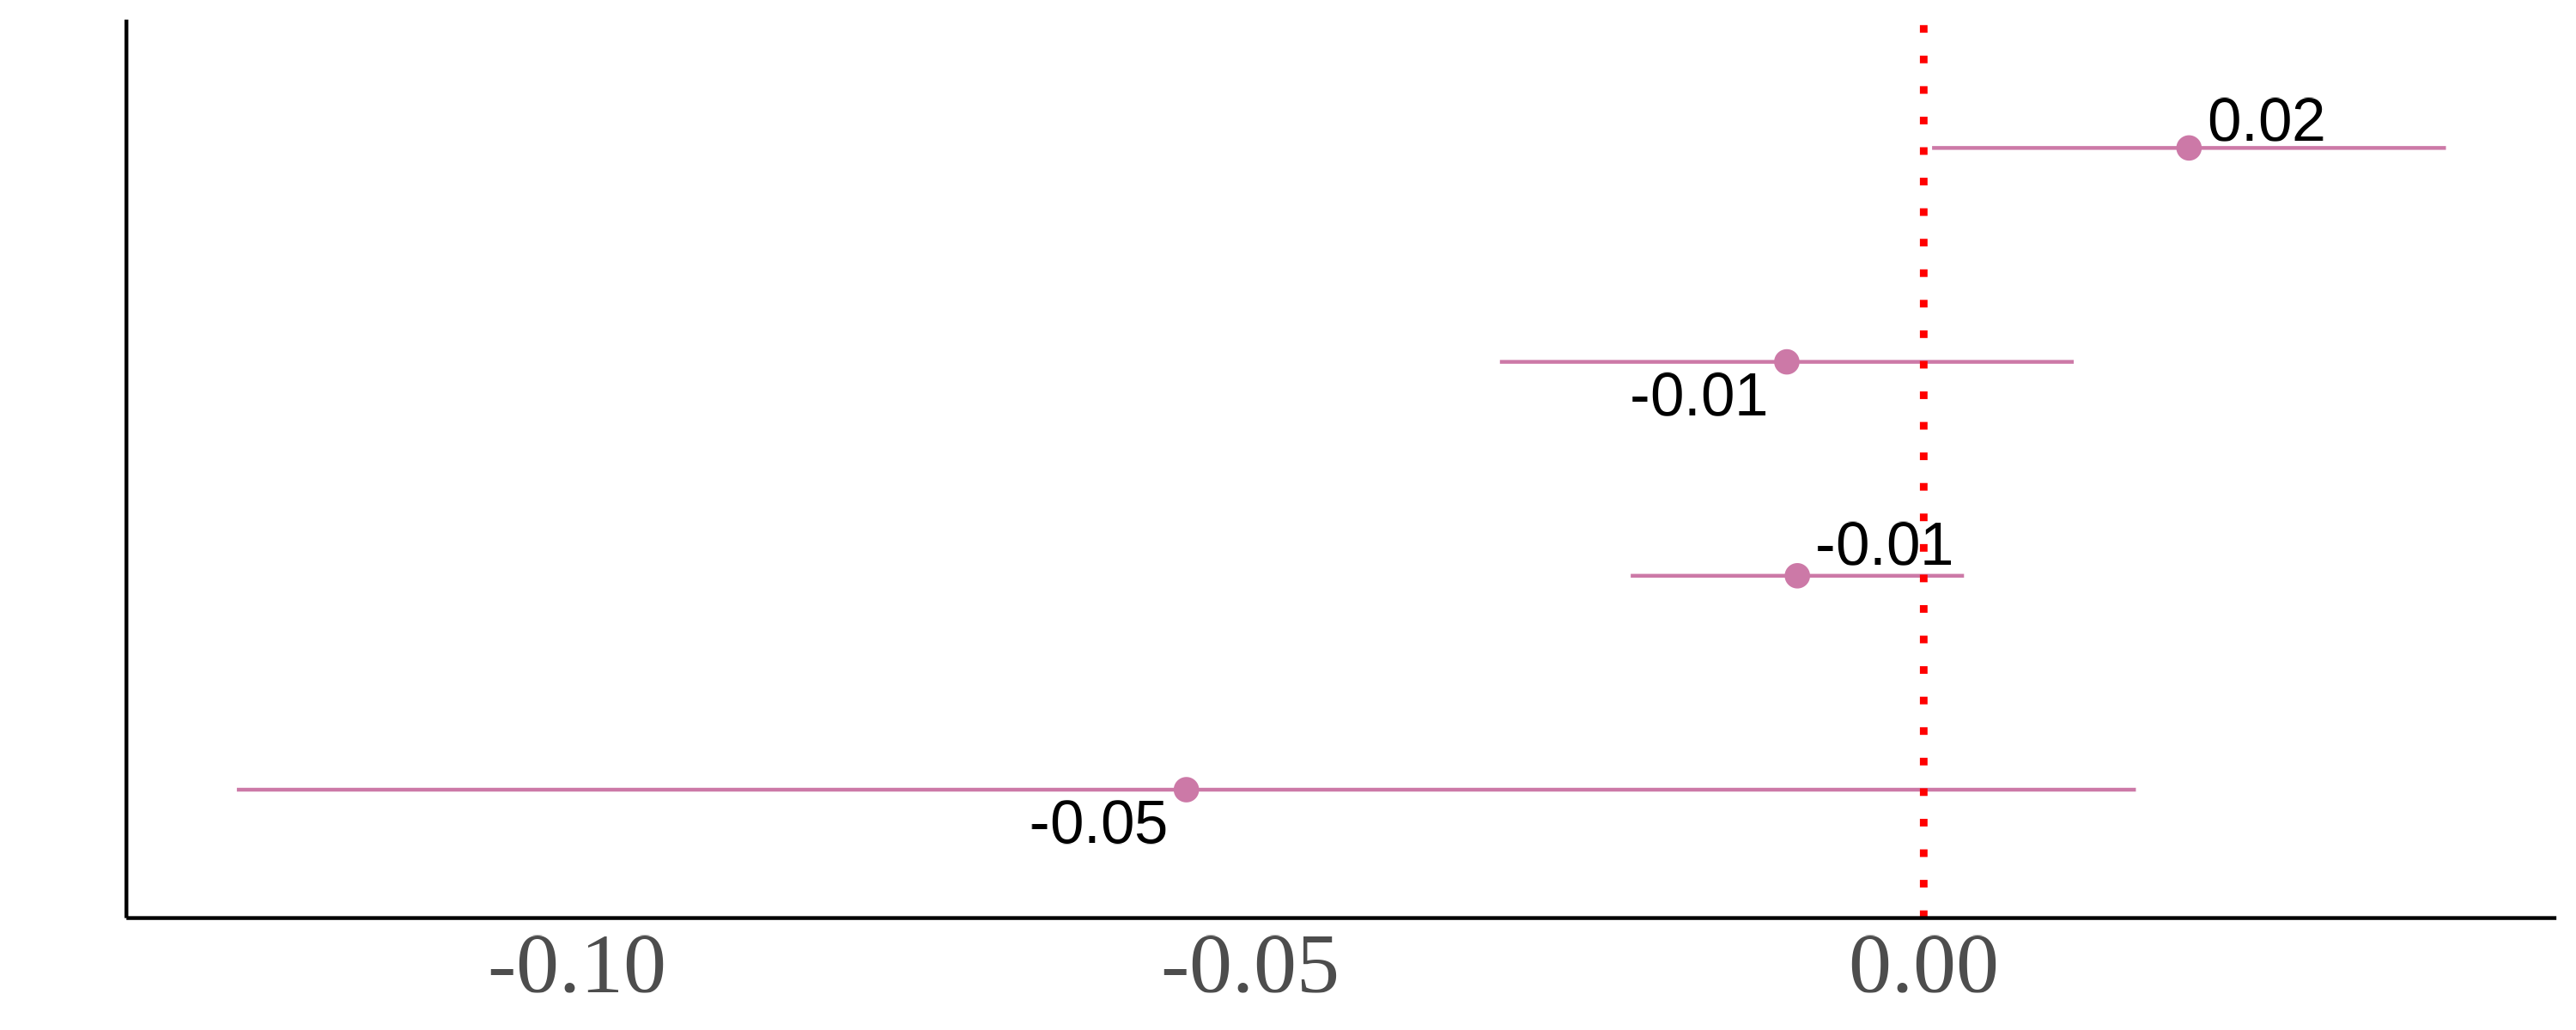
\includegraphics[width=.9\linewidth]{skin-iat-regression-first-gen.png}
\end{subfigure}
%Third Graph
\begin{subfigure}{.48\textwidth}
\caption{Second-Generation}
\centering
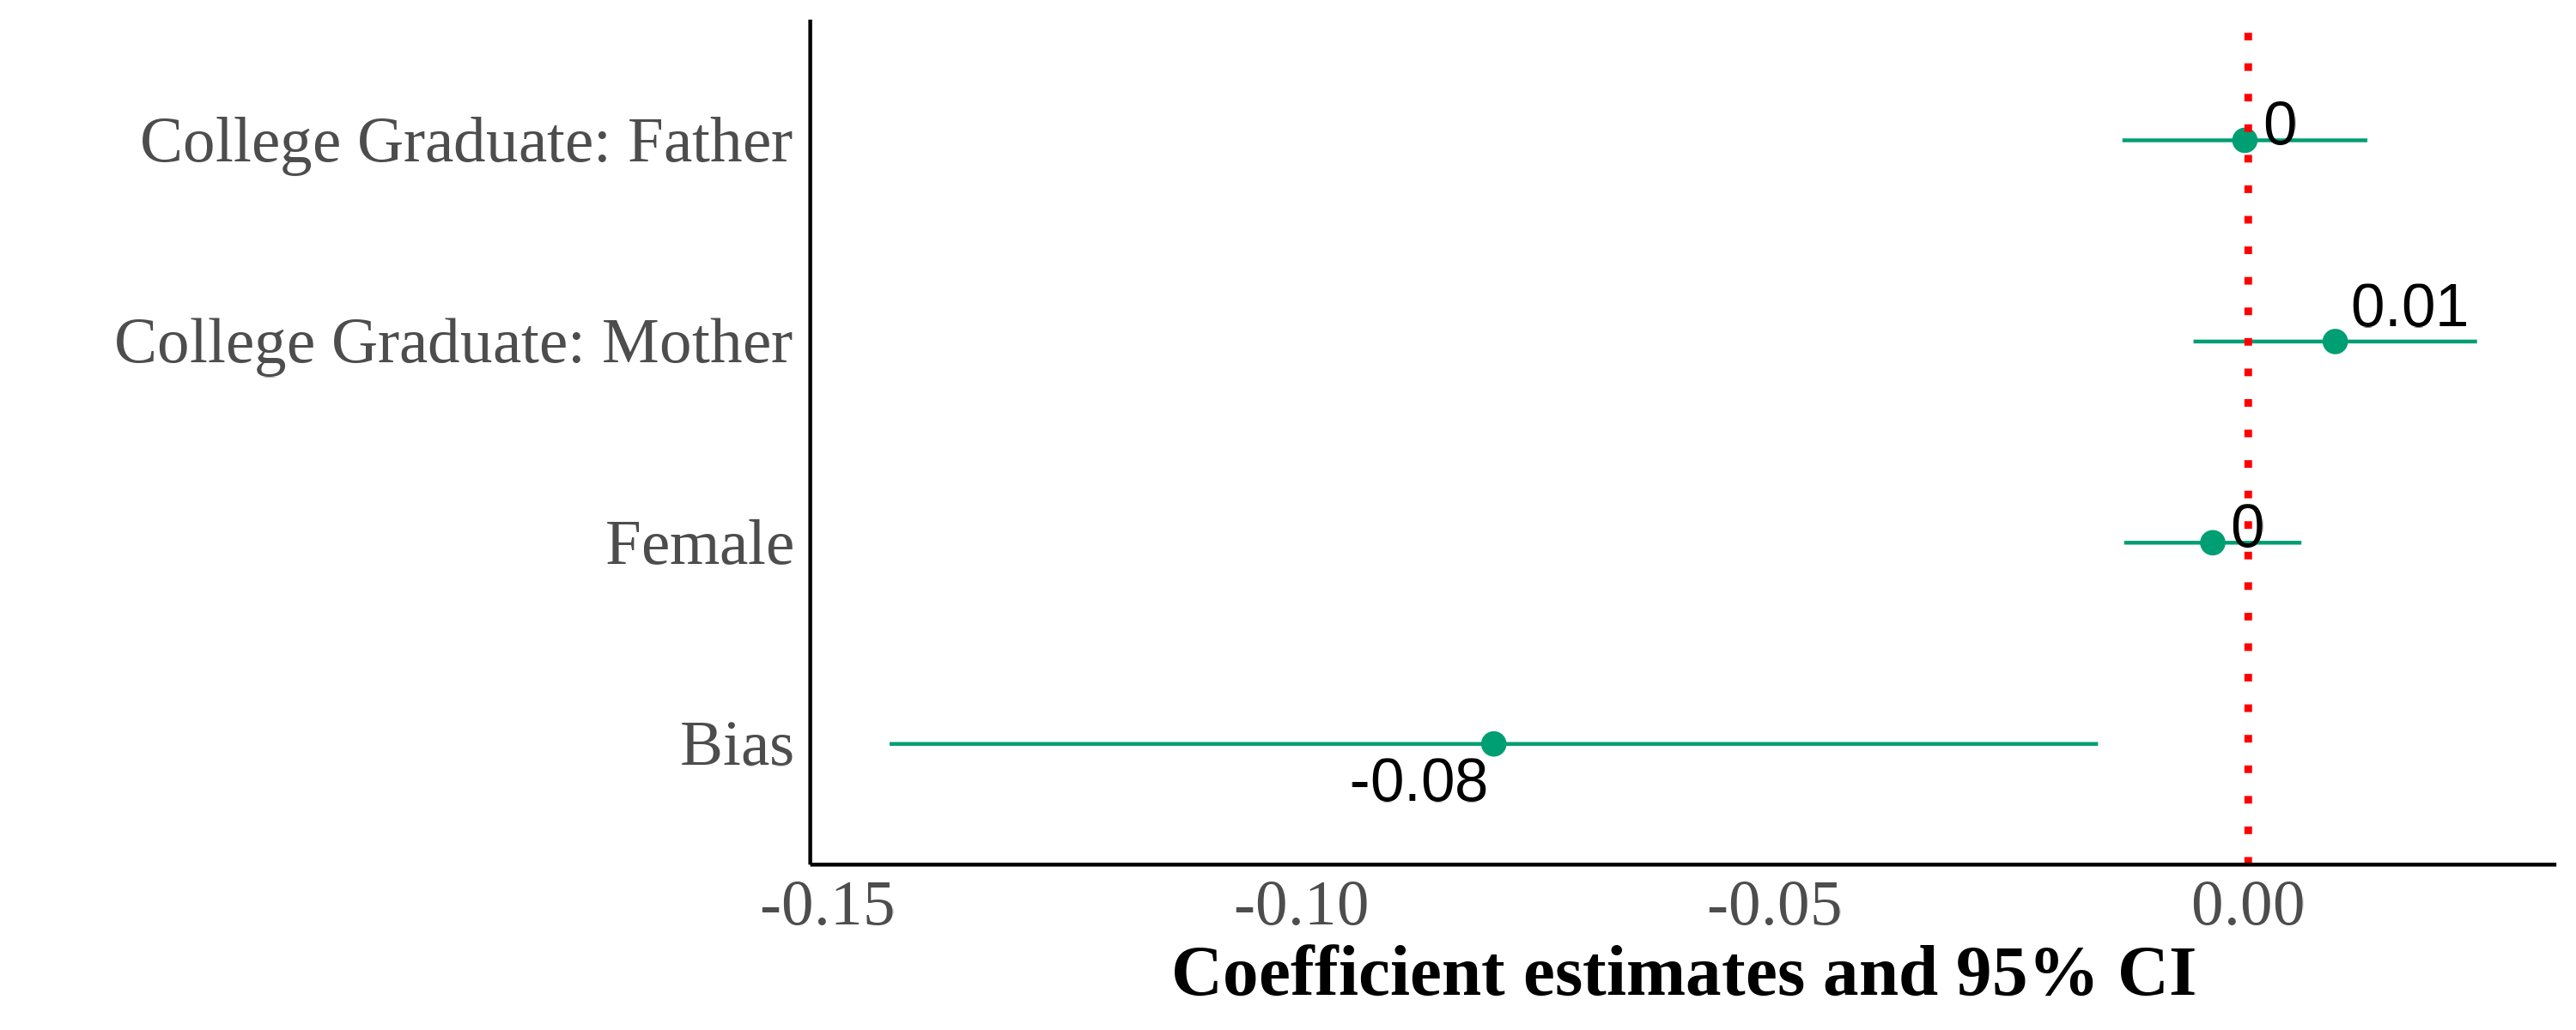
\includegraphics[width=.9\linewidth]{skin-iat-regression-second-gen.png}
\end{subfigure}
%Fourth Graph
\begin{subfigure}{.48\textwidth}
\caption{Third-Generation}
\centering
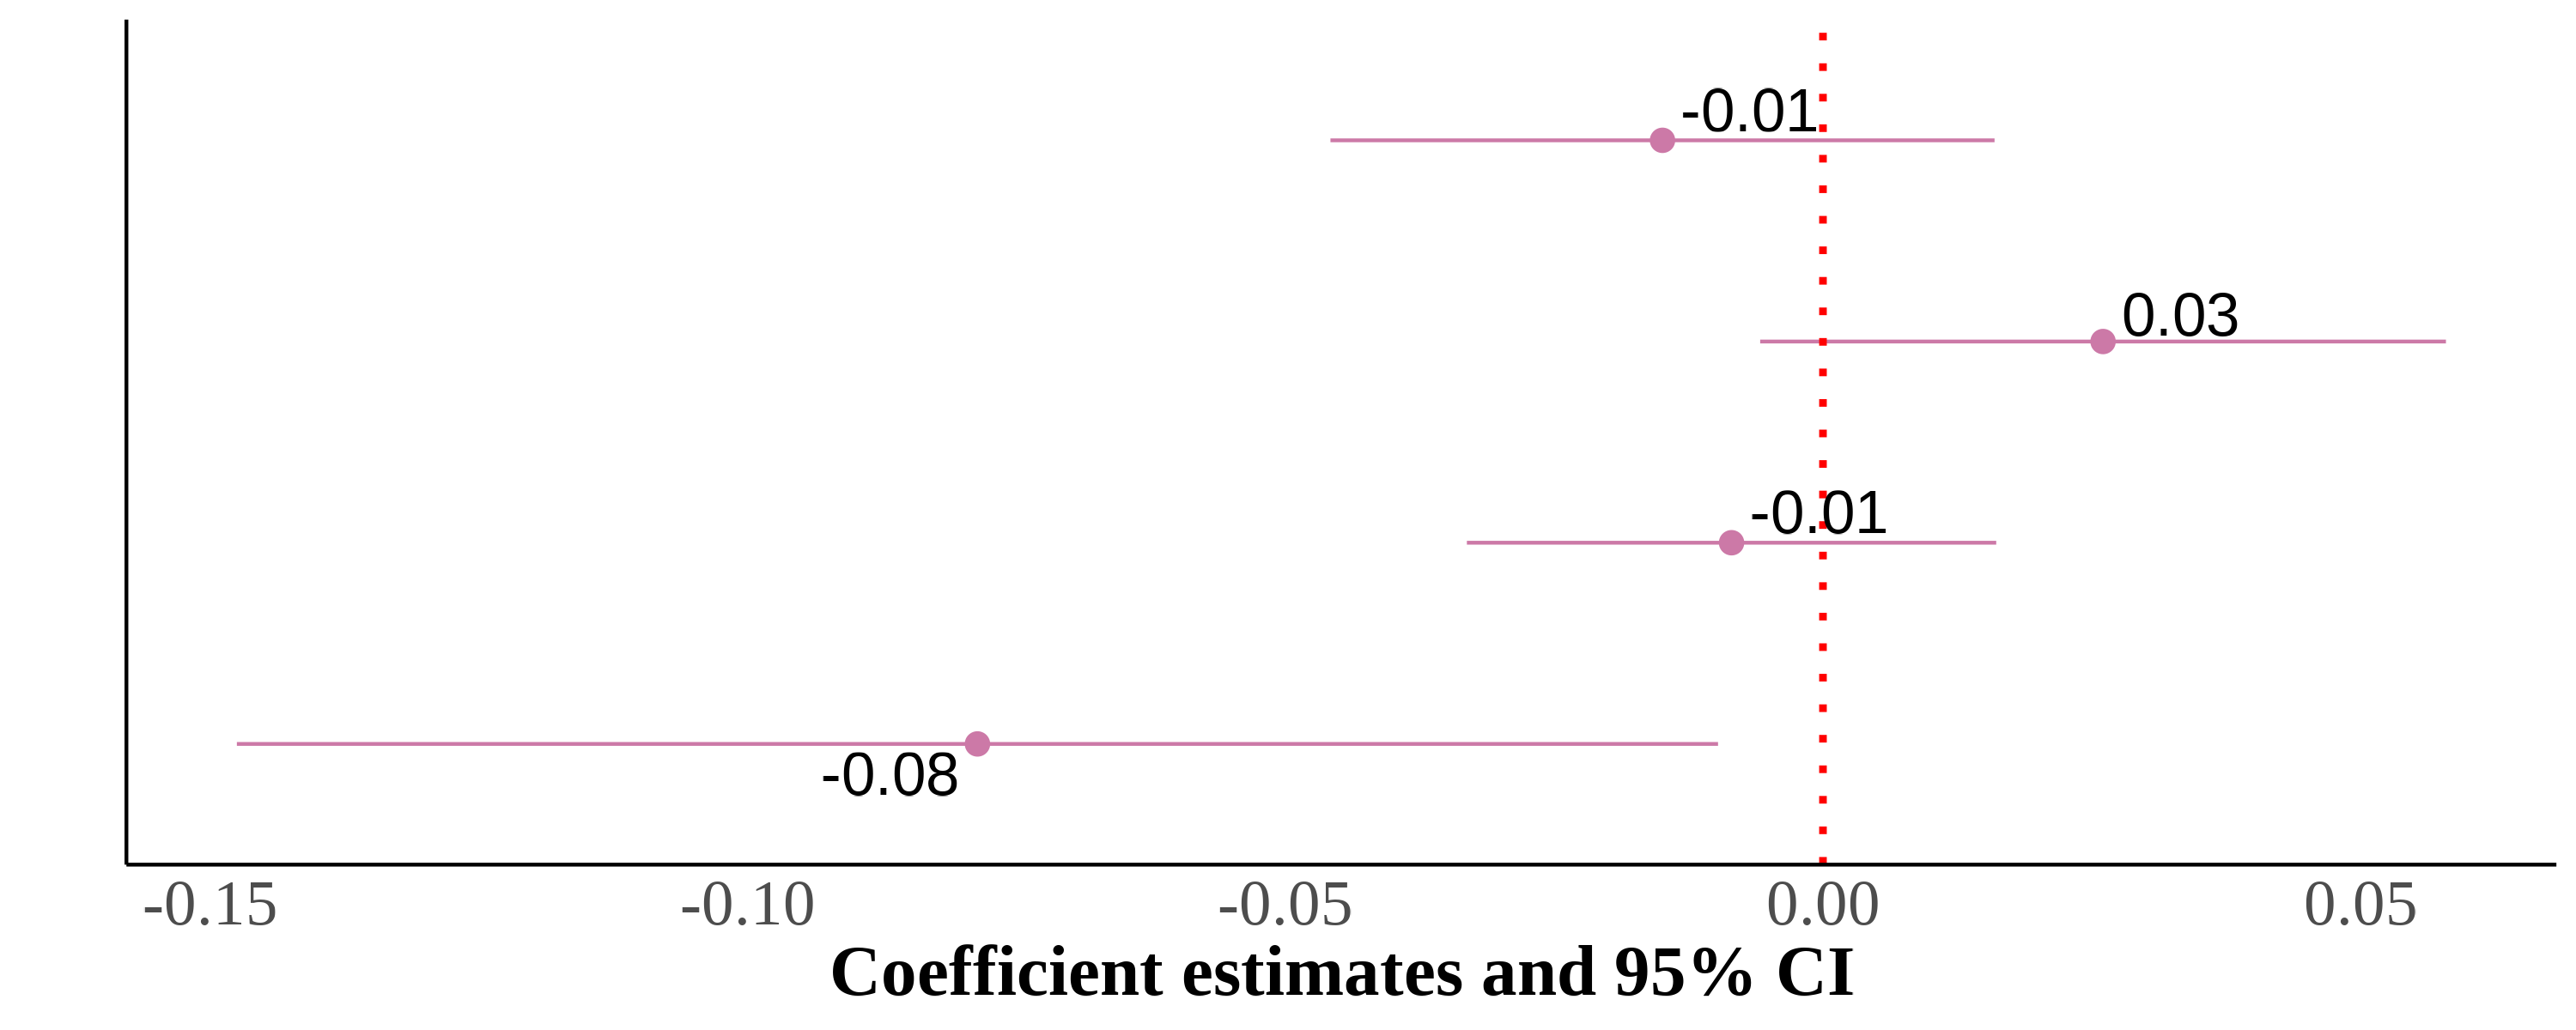
\includegraphics[width=.9\linewidth]{skin-iat-regression-third-gen.png}
\end{subfigure}
\caption*{\footnotesize{I show four panels of estimating equation (\ref{eq:identity_reg_bias}). I include region $\times$ year fixed effects with controls for sex, quartic age, and parental education. The dependent variable is self-reported Asian identity and the independent variable is state-level bias. Each panel is the results from the same regression but on different samples that are divided by generation. Standard errors are clustered on the state level. The samples include first-, second-, and third-generation Asian children ages 17 and below who live in intact families. First-generation Asian immigrants are children that were born in a Asian country. Native-born second-generation Asian immigrants are children with at least one parent born in a Asian country. Finally, native-born third-generation Asian immigrants are children with native-born parents and at least one grandparent born in a Asian country.}}
\end{figure}
\end{center}

\pagebreak
\newpage

\begin{center}
\begin{figure}[!htb]
\centering
\caption{Relationship Between Self-Reported Asian Identity and Bias: By Generation Among Adults}
\label{plot01-regression-gen-adults}
%First graph
\begin{subfigure}{.48\textwidth}
\caption{All Generations}
\centering
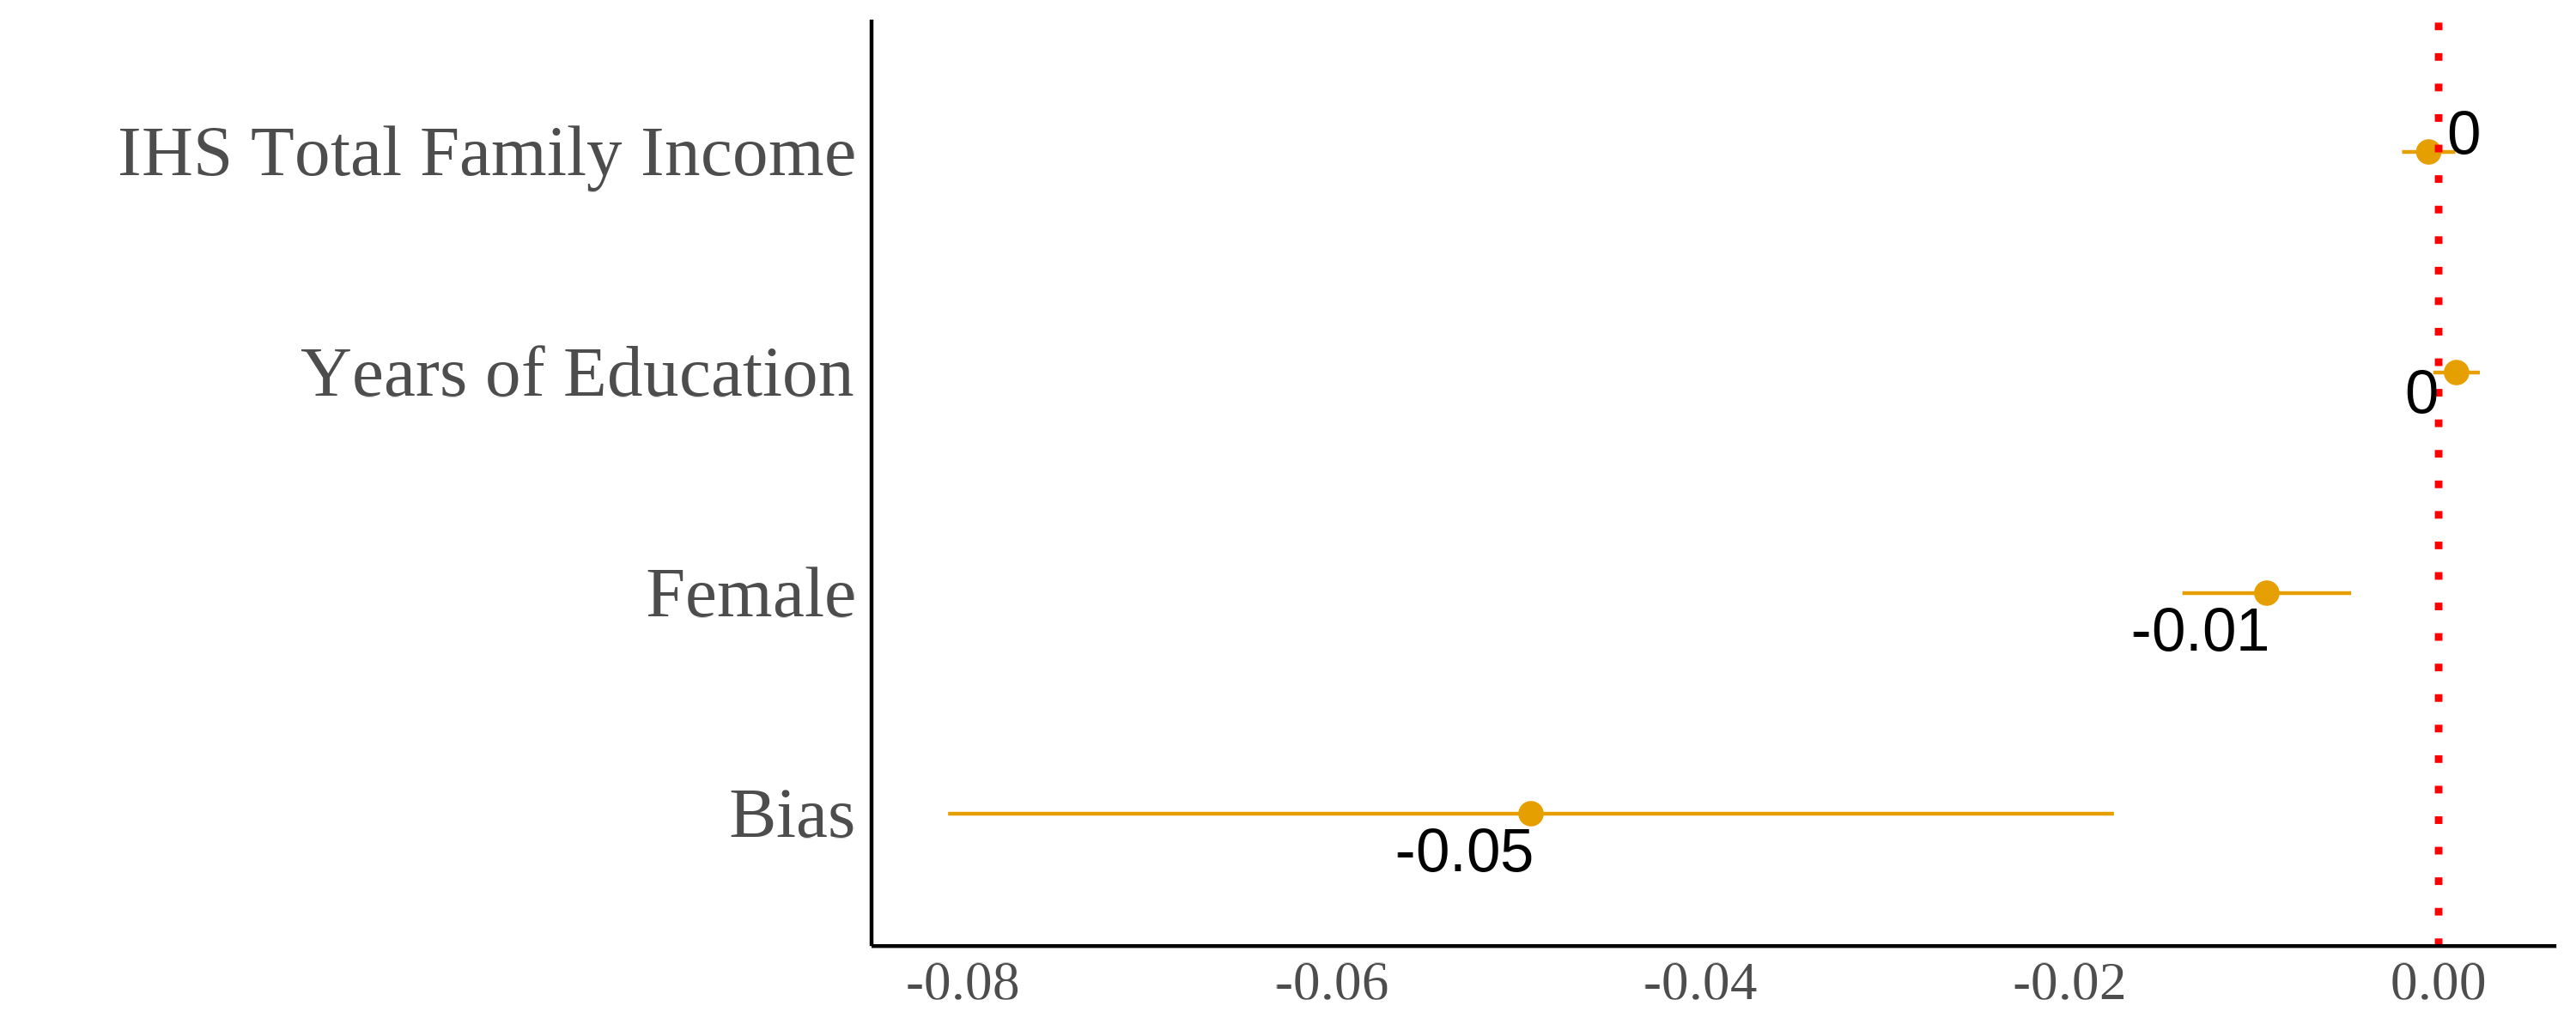
\includegraphics[width=.9\linewidth]{skin-iat-regression-all-gens-adults.png}
\end{subfigure}
\centering
%Second graph
\begin{subfigure}{.48\textwidth}
\caption{First-Generation}
\centering
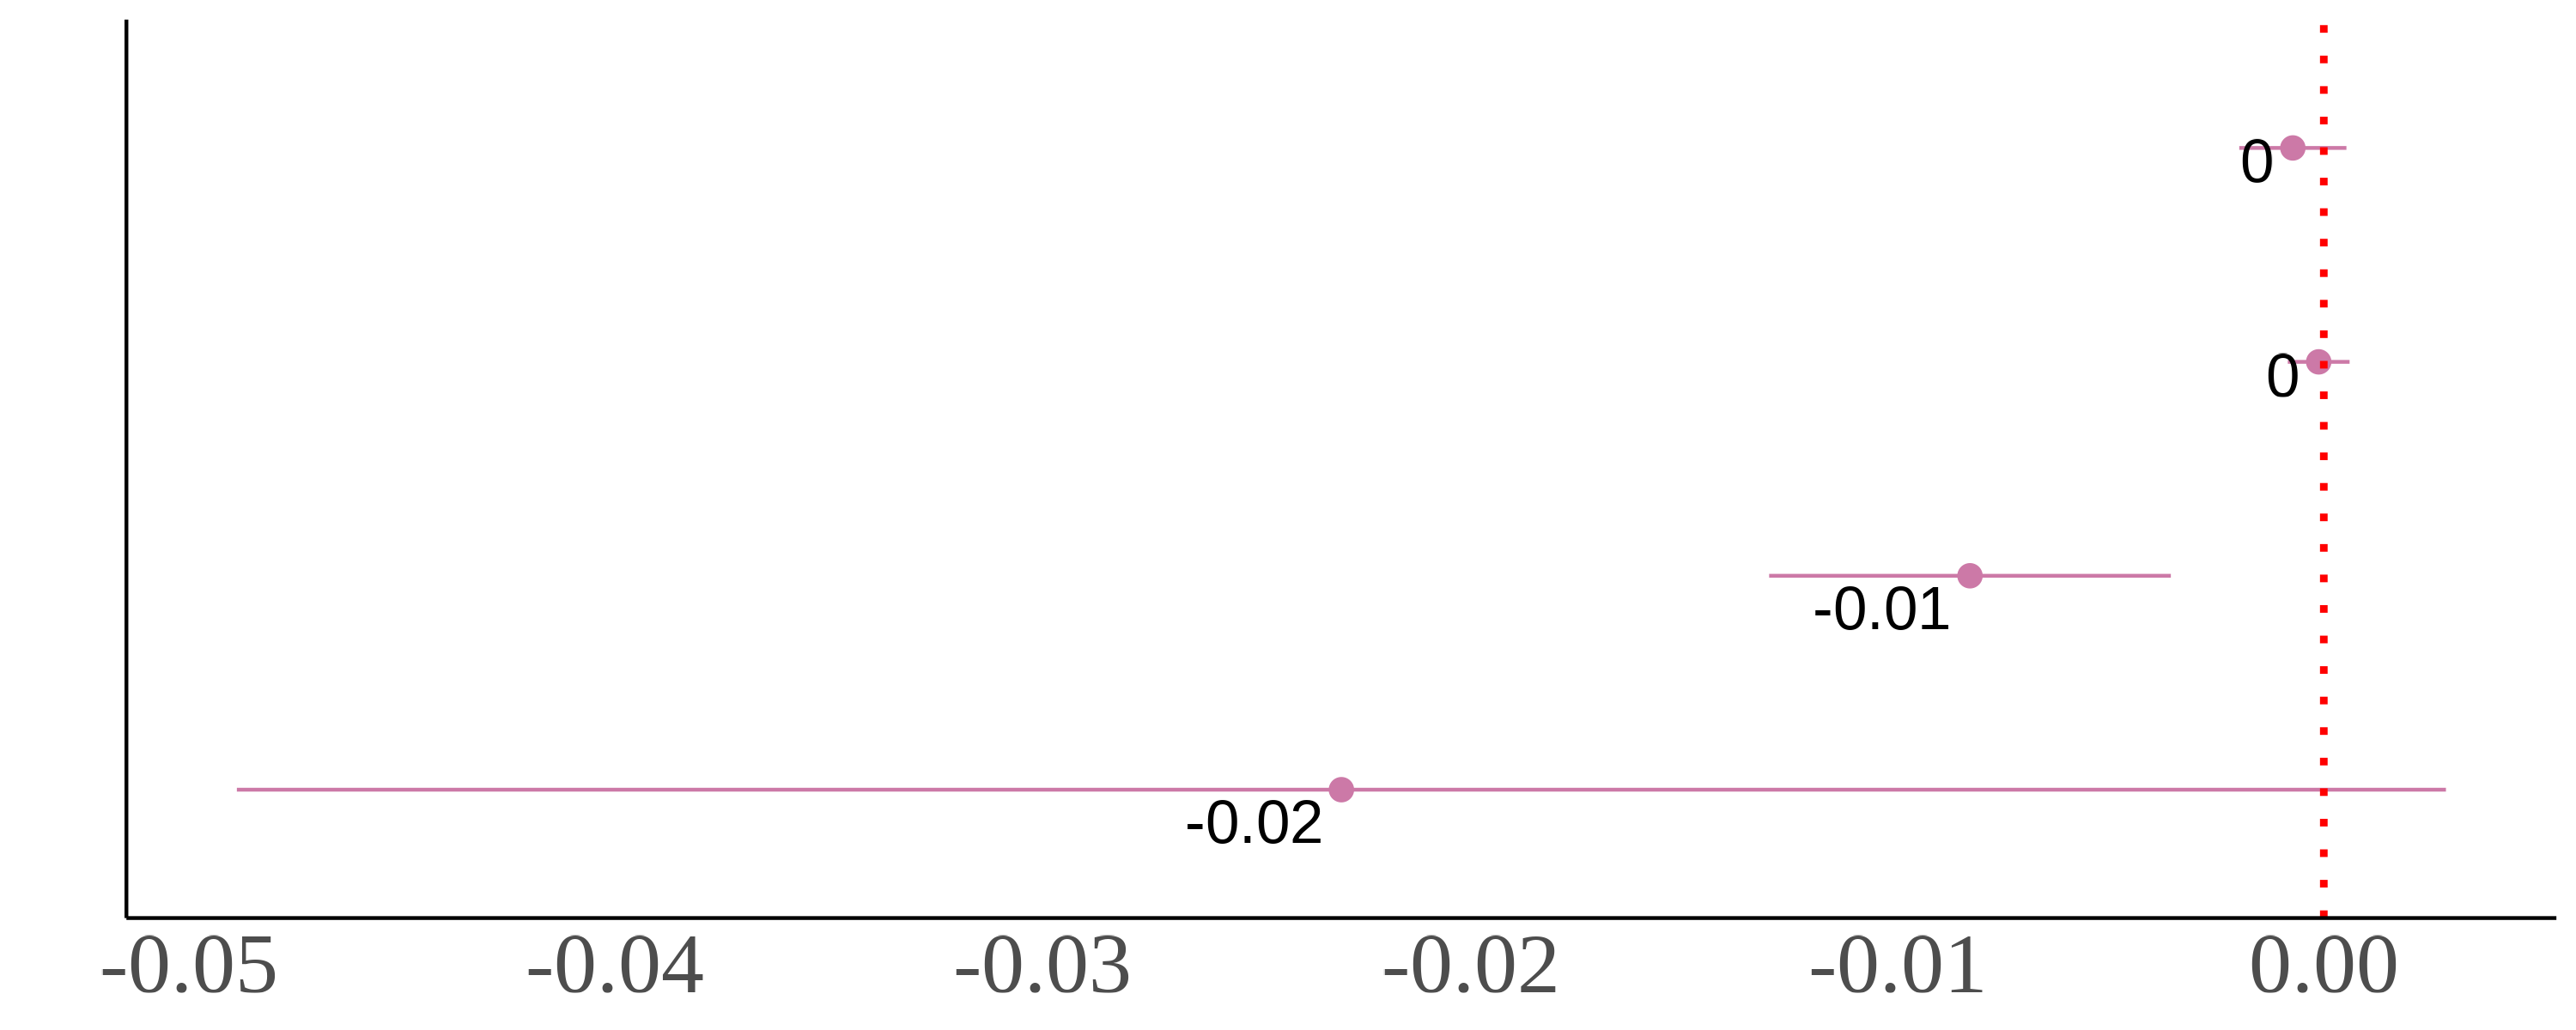
\includegraphics[width=.9\linewidth]{skin-iat-regression-first-gen-adults.png}
\end{subfigure}
%Third Graph
\begin{subfigure}{.48\textwidth}
\caption{Second-Generation}
\centering
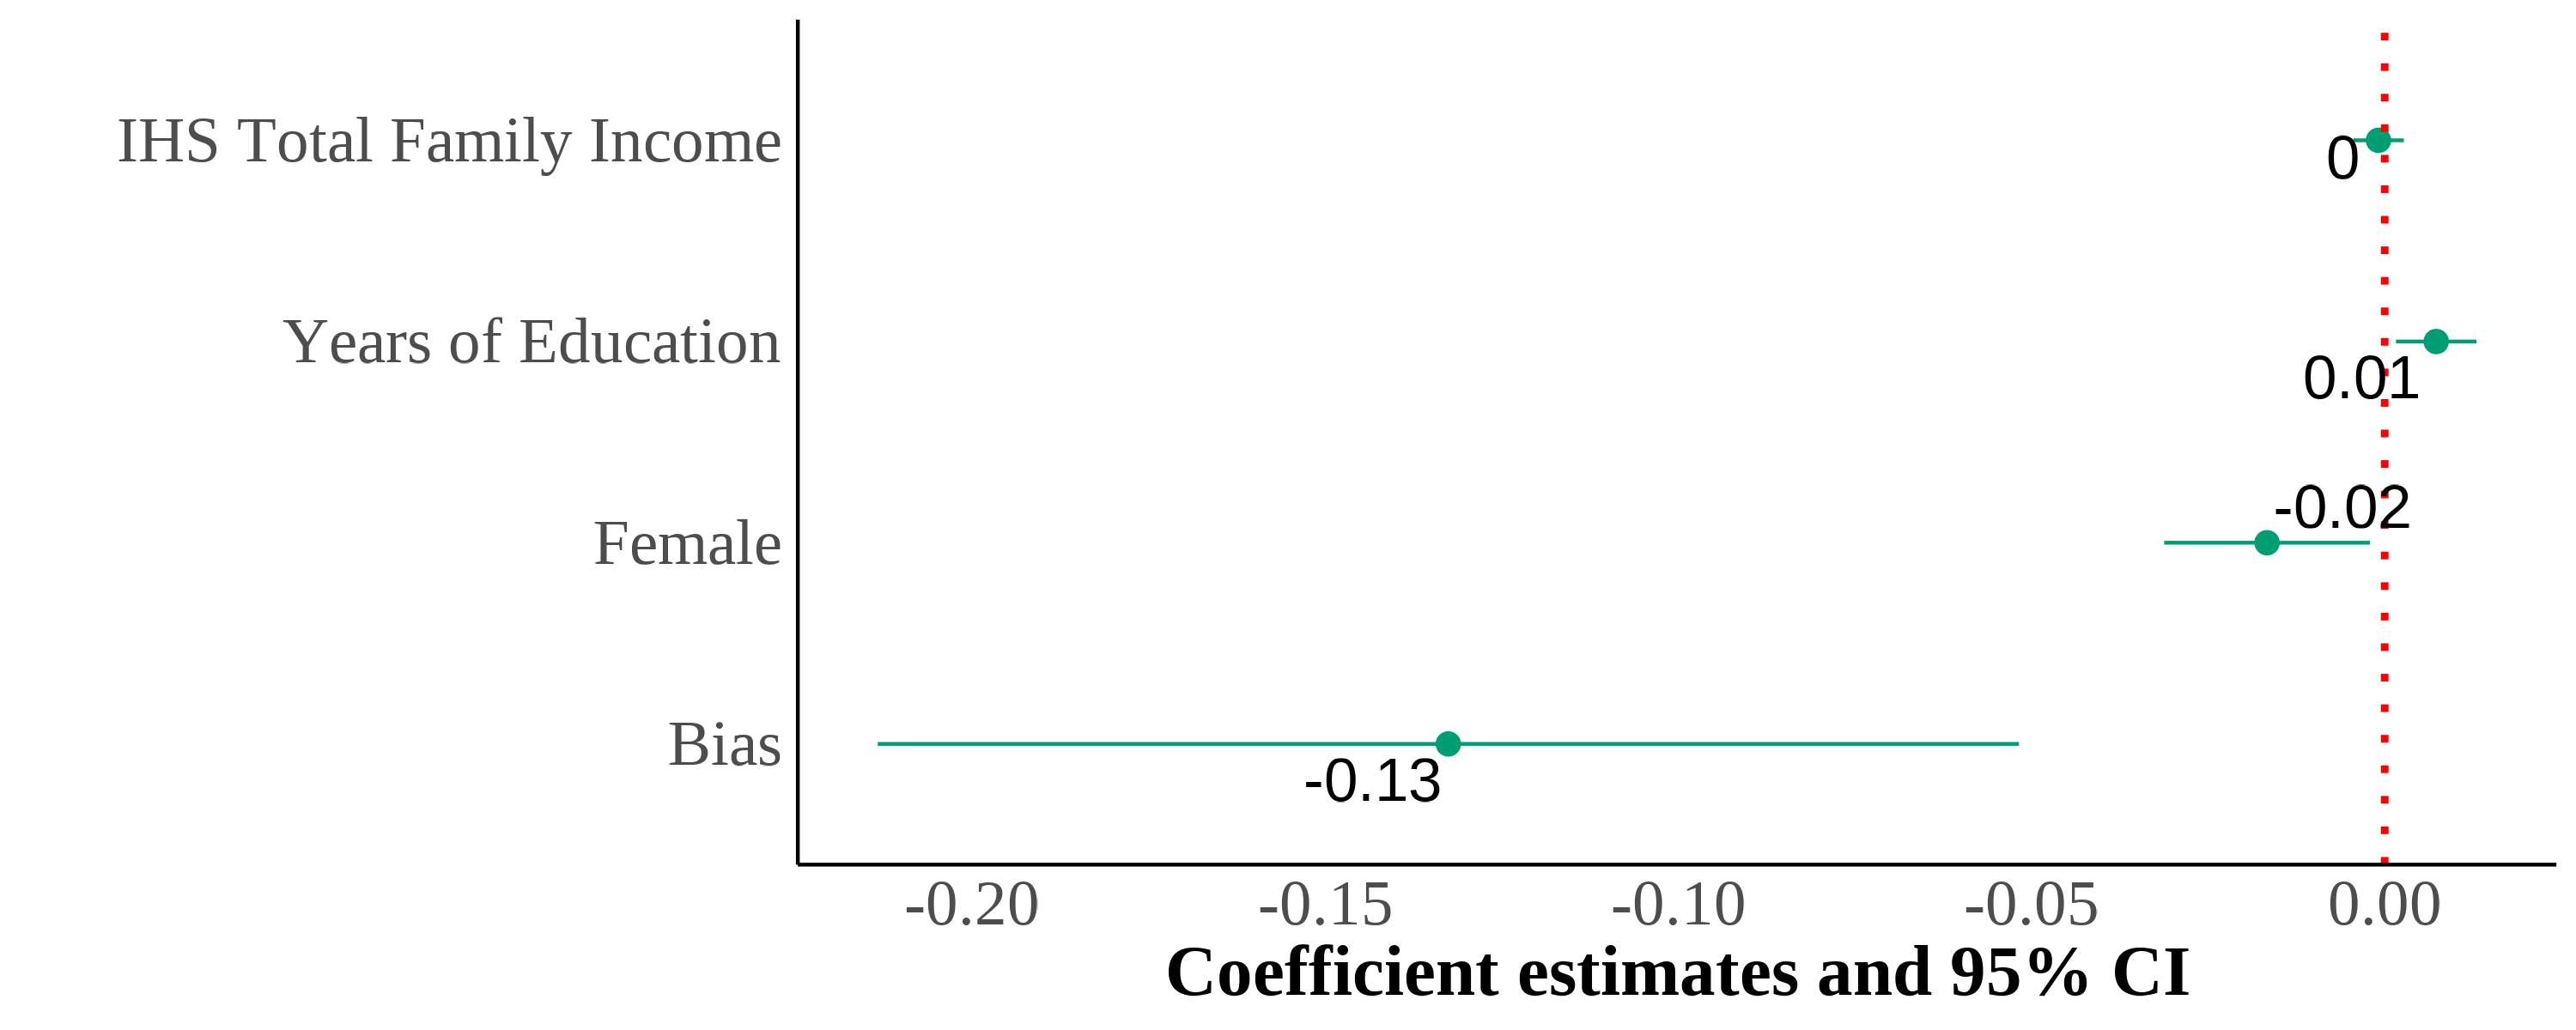
\includegraphics[width=.9\linewidth]{skin-iat-regression-second-gen-adults.png}
\end{subfigure}

\caption*{\footnotesize{I show three panels of estimating equation (\ref{eq:identity_reg_bias}) on a sample of adults. I include region $\times$ year fixed effects with controls for sex, quartic age, years of education, and inverse hyperbolic sine of income. The dependent variable is self-reported Asian identity and the independent variable is state-level bias. Each panel is the results from the same regression but on different samples that are divided by generation. Standard errors are clustered on the state level. The samples include first- and second-generation Asian adults ages 18 and above. First-generation Asian immigrants are individuals that were born in a Asian country. Native-born second-generation Asian immigrants are individuals with at least one parent born in a Asian country.}}
\end{figure}
\end{center}

\pagebreak
\newpage

\begin{center}
\begin{figure}[!htb]
\centering
\caption{Relationship Between Self-Reported Asian Identity and Bias: By Parental Types}
\label{plot01-regression-byparent}
%First graph
\begin{subfigure}{.48\textwidth}
\caption{Second-Generation (All Parental Types)}
\centering
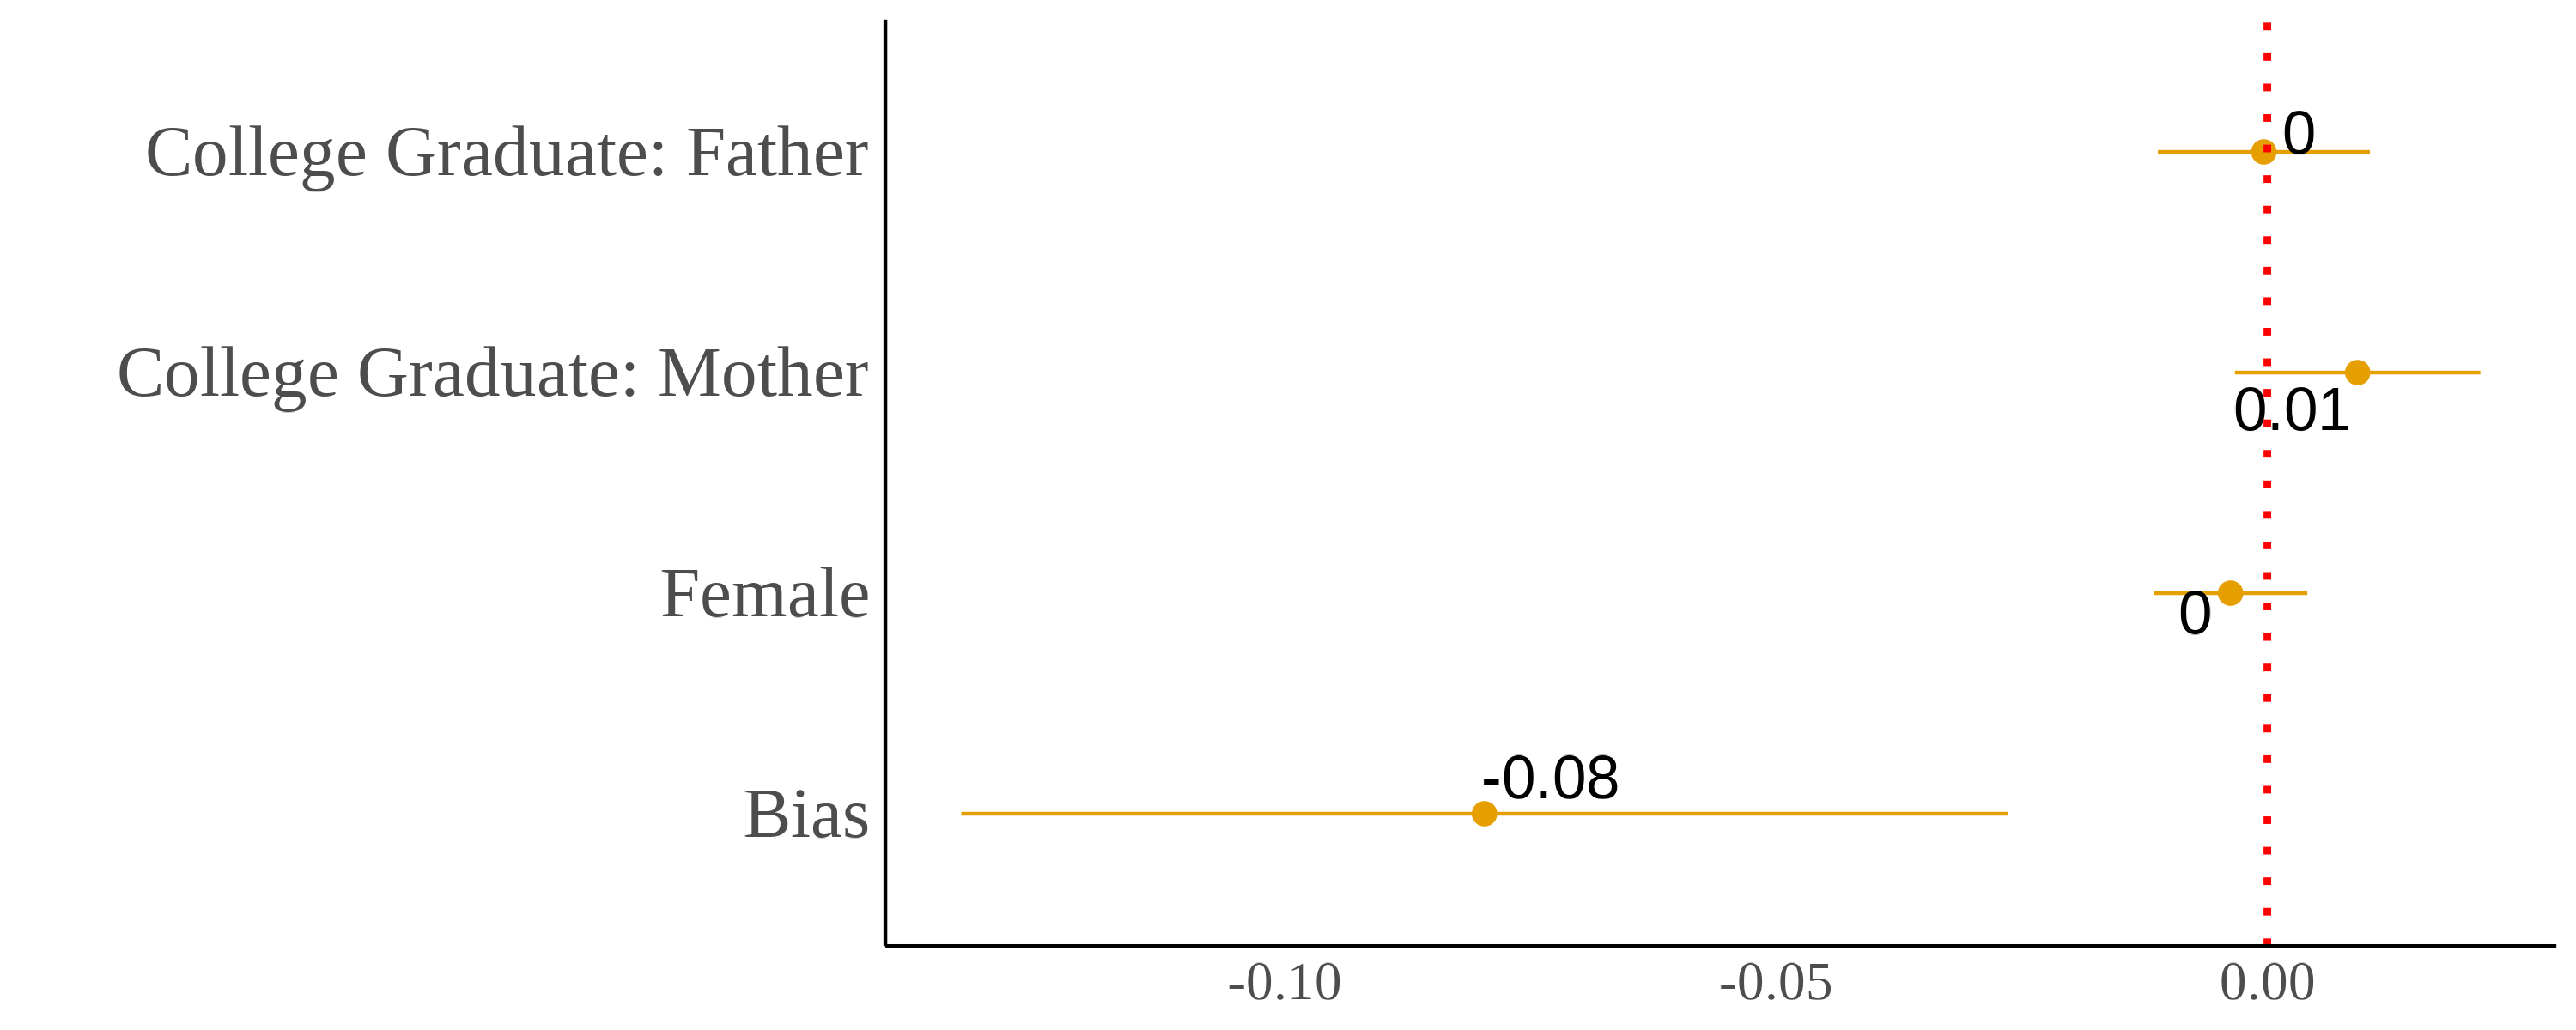
\includegraphics[width=.9\linewidth]{by-parents-regs-all.png}
\end{subfigure}
\centering
%Second graph
\begin{subfigure}{.48\textwidth}
\caption{Asian Fathers-Asian Mothers}
\centering
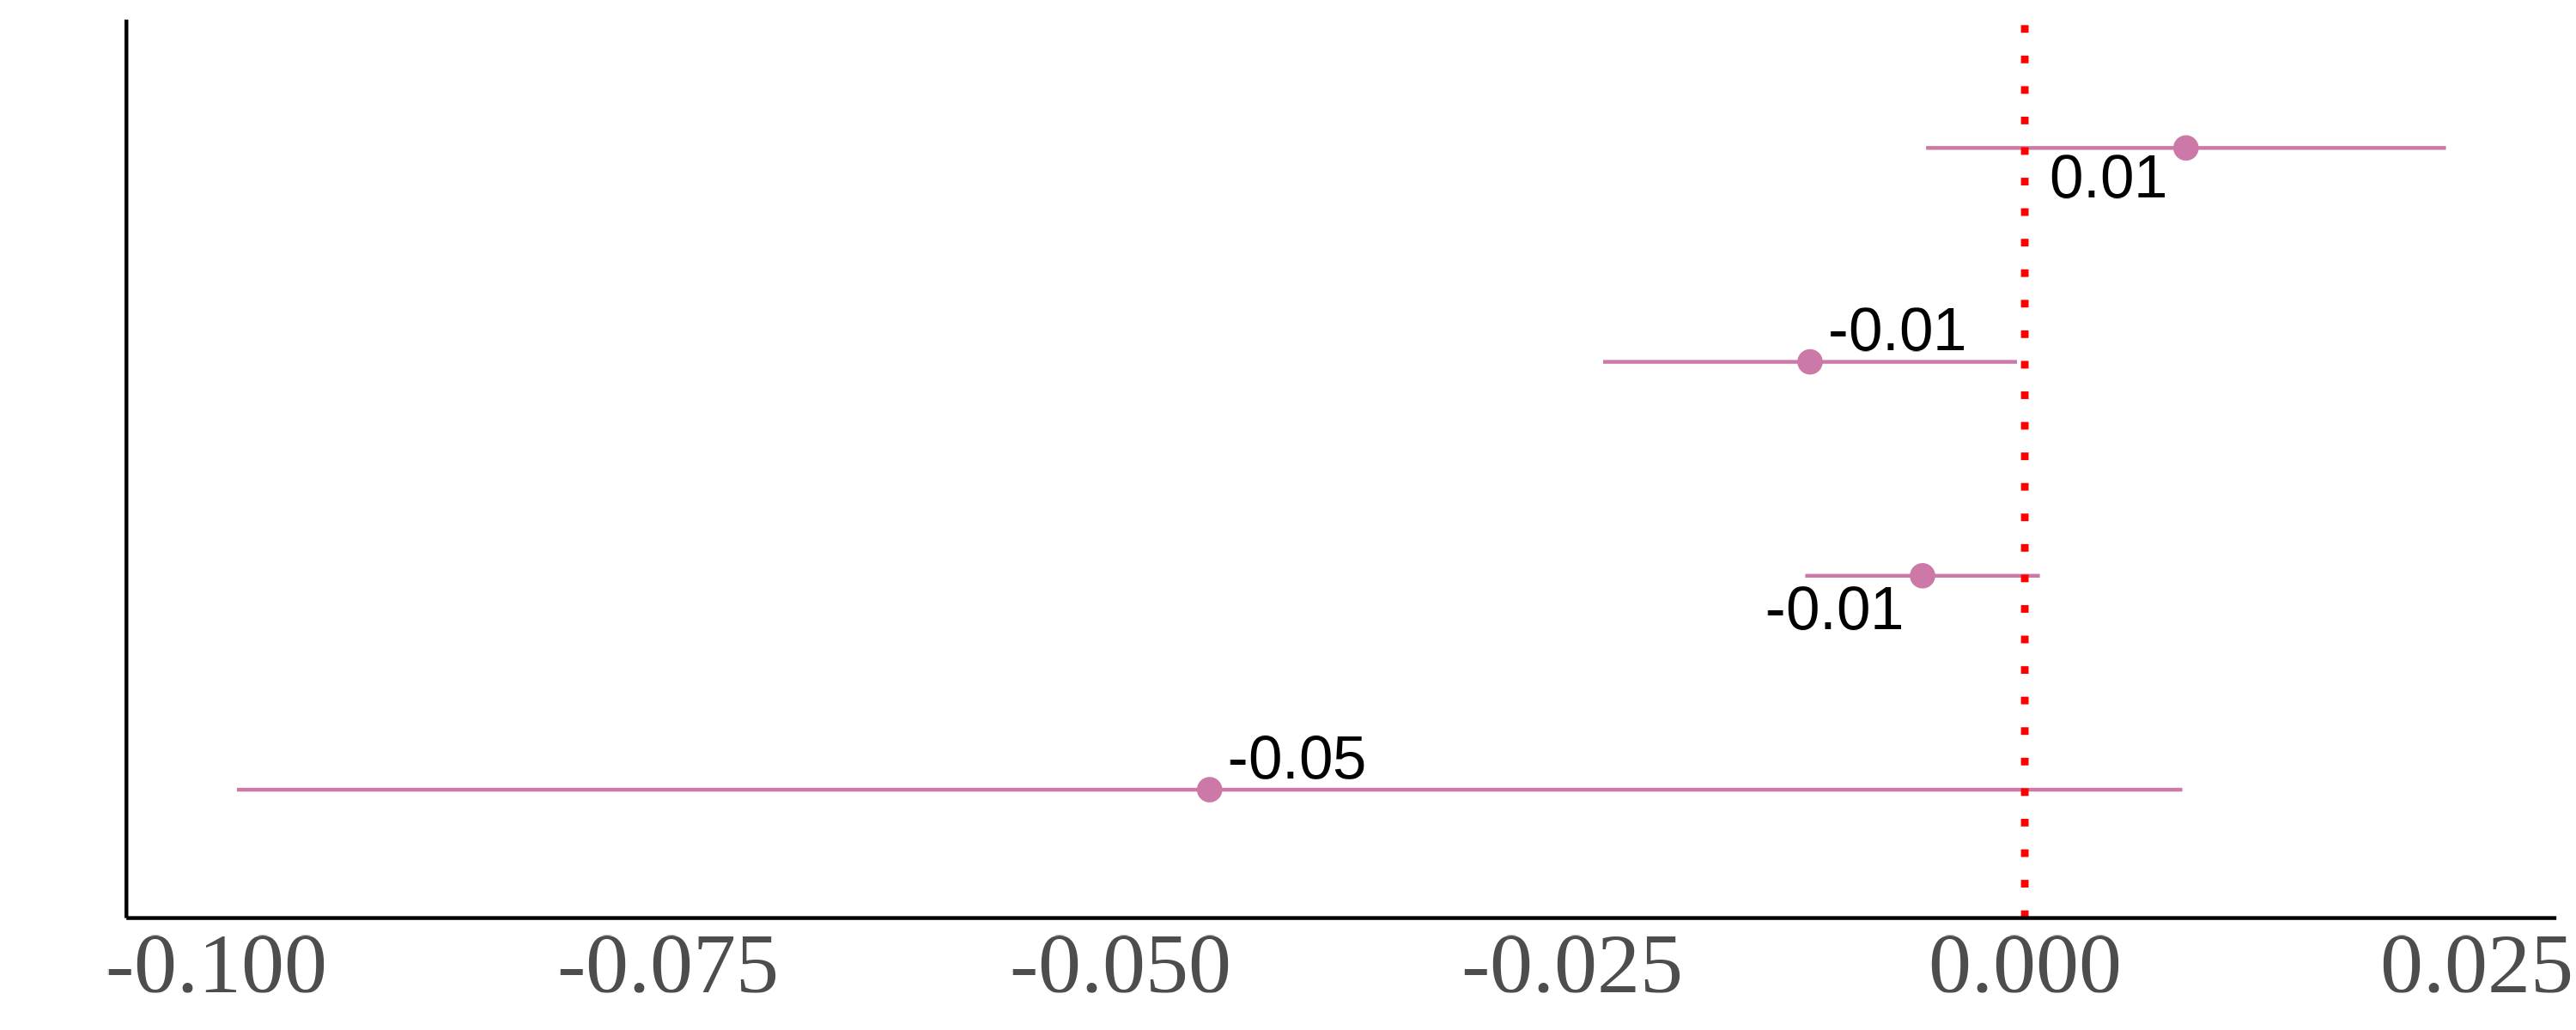
\includegraphics[width=.9\linewidth]{by-parents-regs-hh.png}
\end{subfigure}
%Third Graph
\begin{subfigure}{.48\textwidth}
\caption{Asian Fathers-White Mothers}
\centering
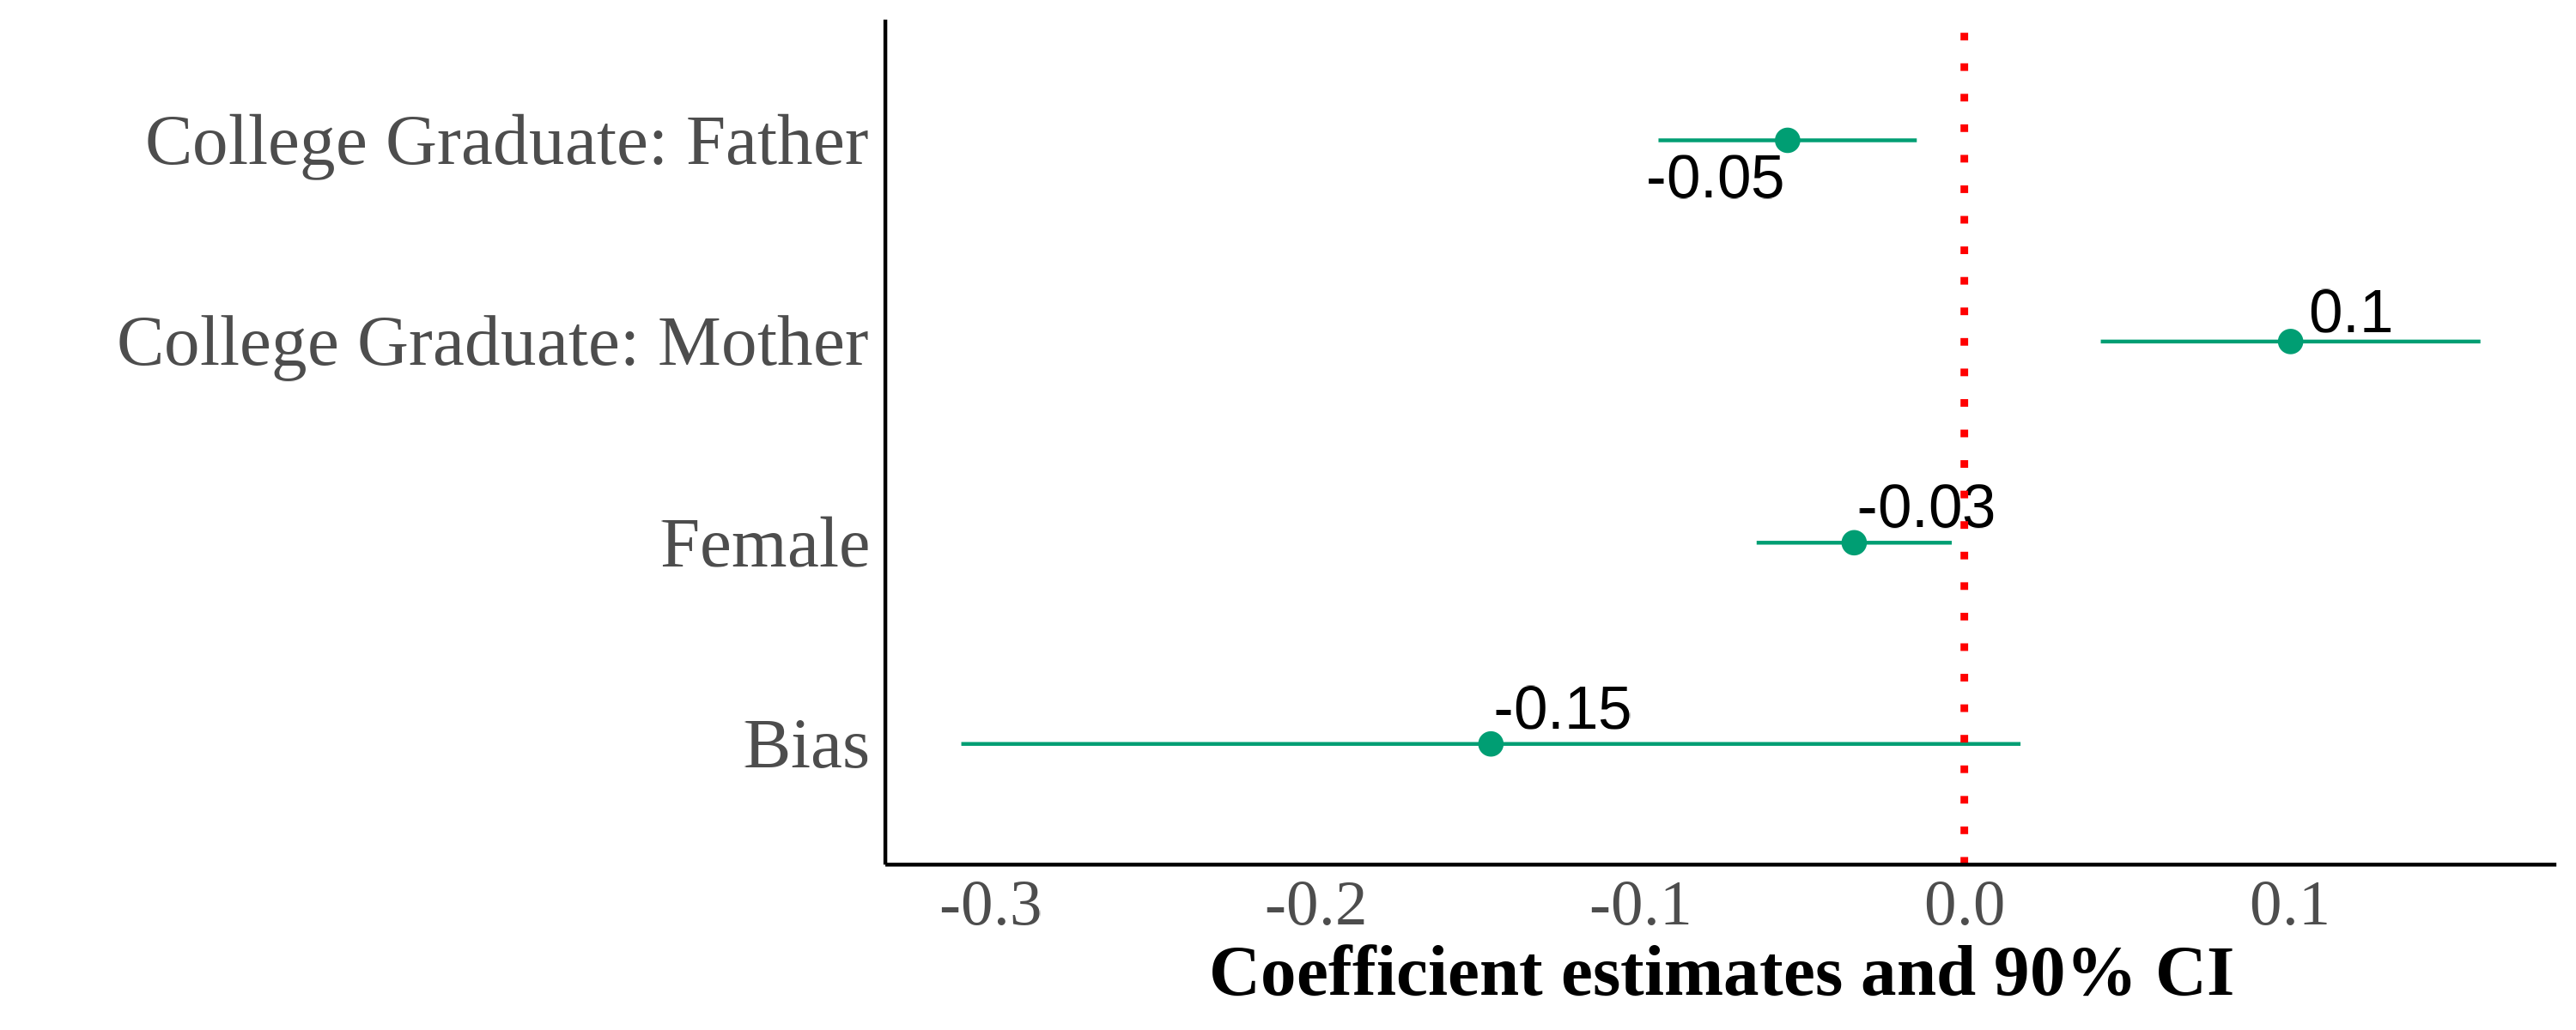
\includegraphics[width=.9\linewidth]{by-parents-regs-hw.png}
\end{subfigure}
%Fourth Graph
\begin{subfigure}{.48\textwidth}
\caption{White Fathers-Asian Mothers}
\centering
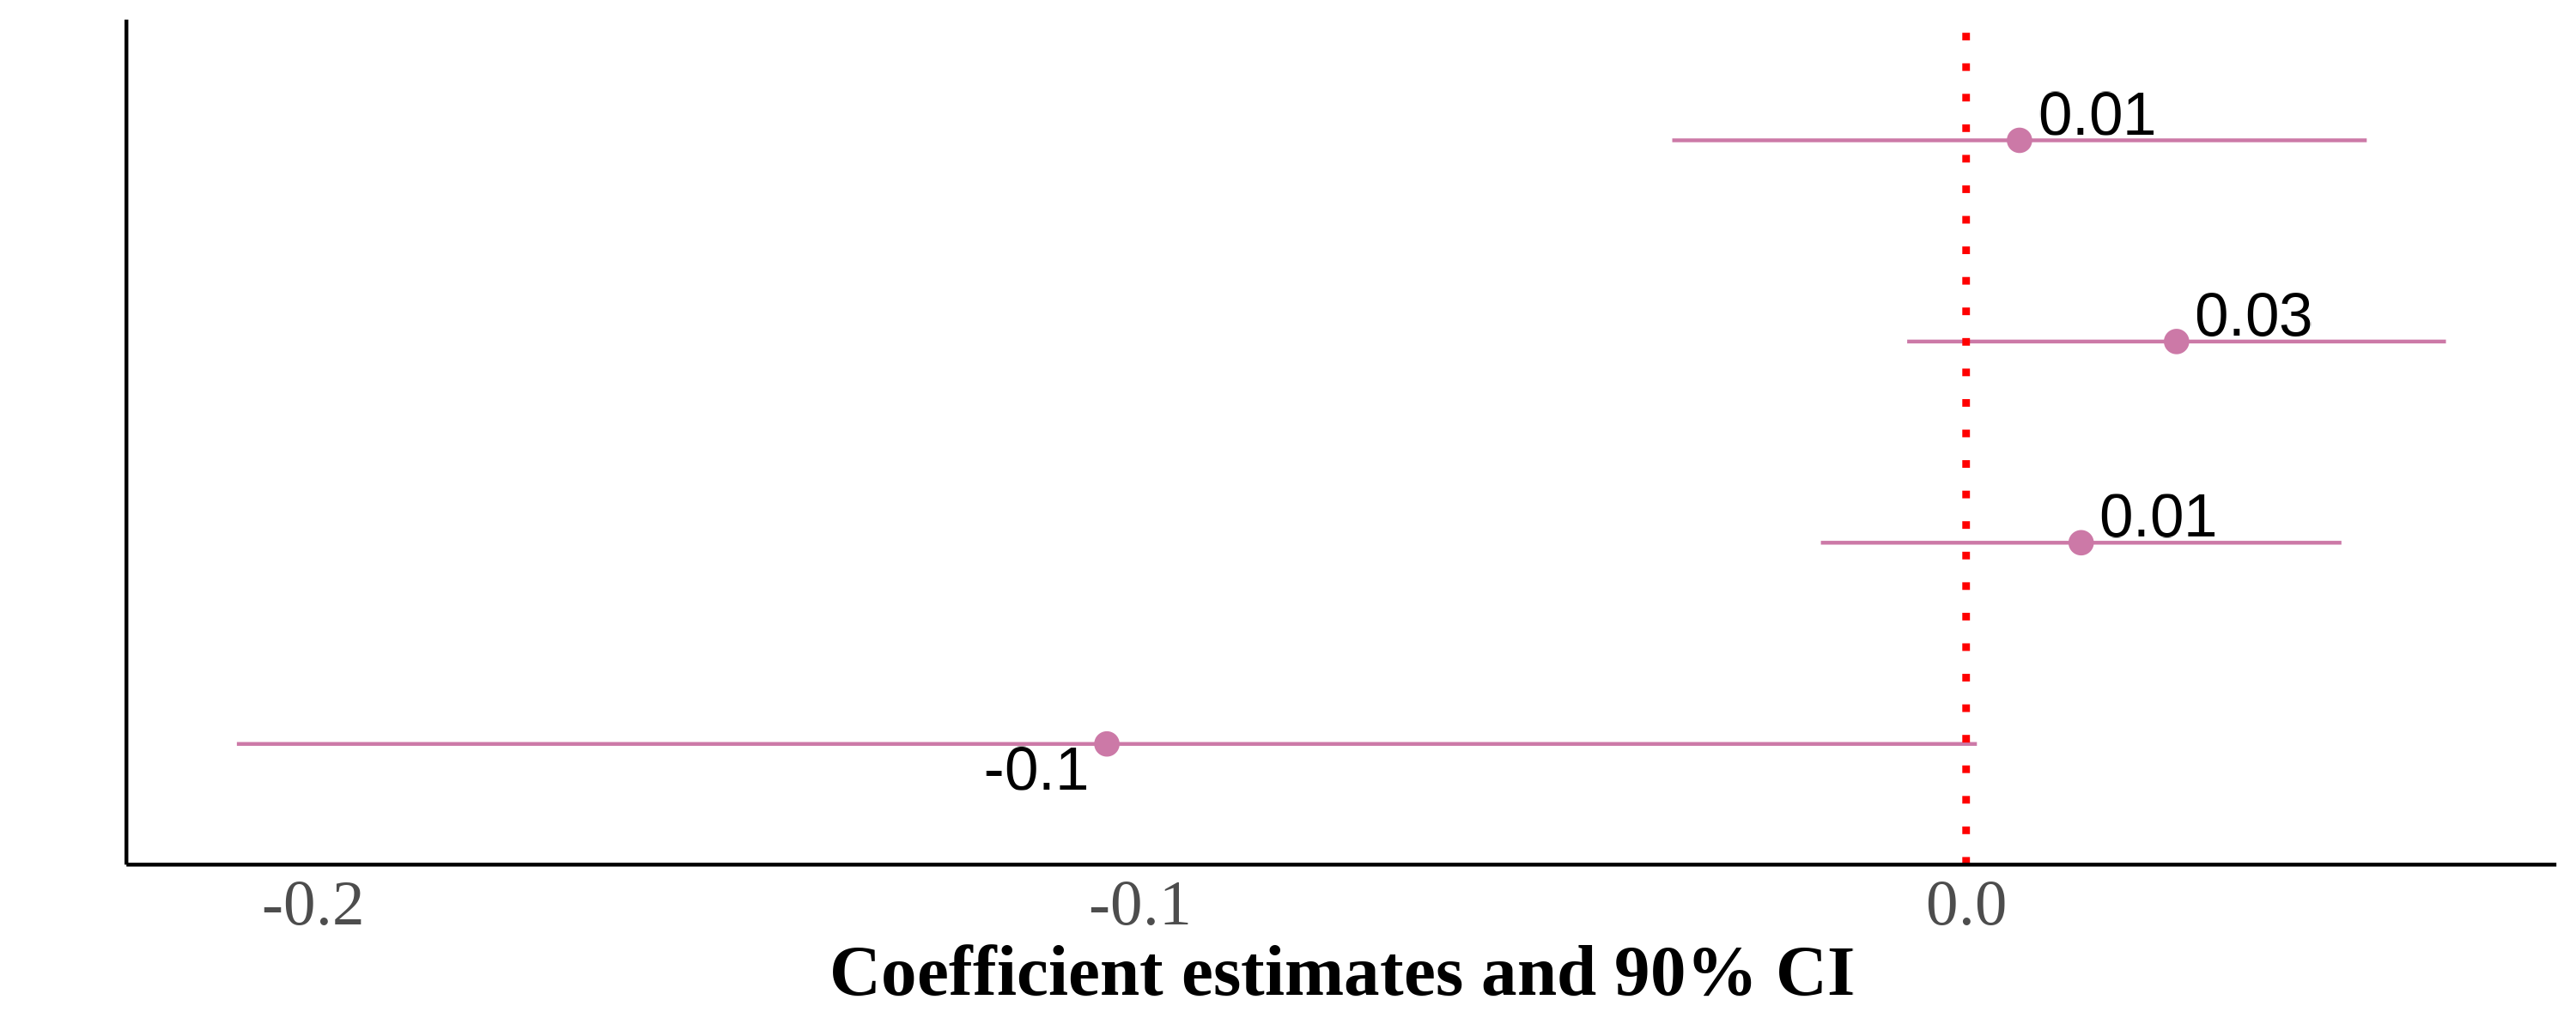
\includegraphics[width=.9\linewidth]{by-parents-regs-wh.png}
\end{subfigure}
\caption*{\footnotesize{I show four panels of estimating equation (\ref{eq:identity_reg_bias}). I include region $\times$ year fixed effects with controls for sex, quartic age, and parental education. The dependent variable is self-reported Asian identity and the independent variable is state-level bias. Each panel results from the same regression but on different samples divided by parental types. Standard errors are clustered on the state level. The samples include second-generation Asian children ages 17 and below who live in intact families. Native-born second-generation Asian immigrant children with at least one parent born in an Asian country.}}
\end{figure}
\end{center}

\pagebreak
\newpage

\begin{center}
\begin{figure}[!htb]
\centering
\caption{Relationship Between Self-Reported Asian Identity and Bias: By Parental Types Among Adults}
\label{plot01-regression-byparent-adults}
%First graph
\begin{subfigure}{.48\textwidth}
\caption{Second-Generation (All Parental Types)}
\centering
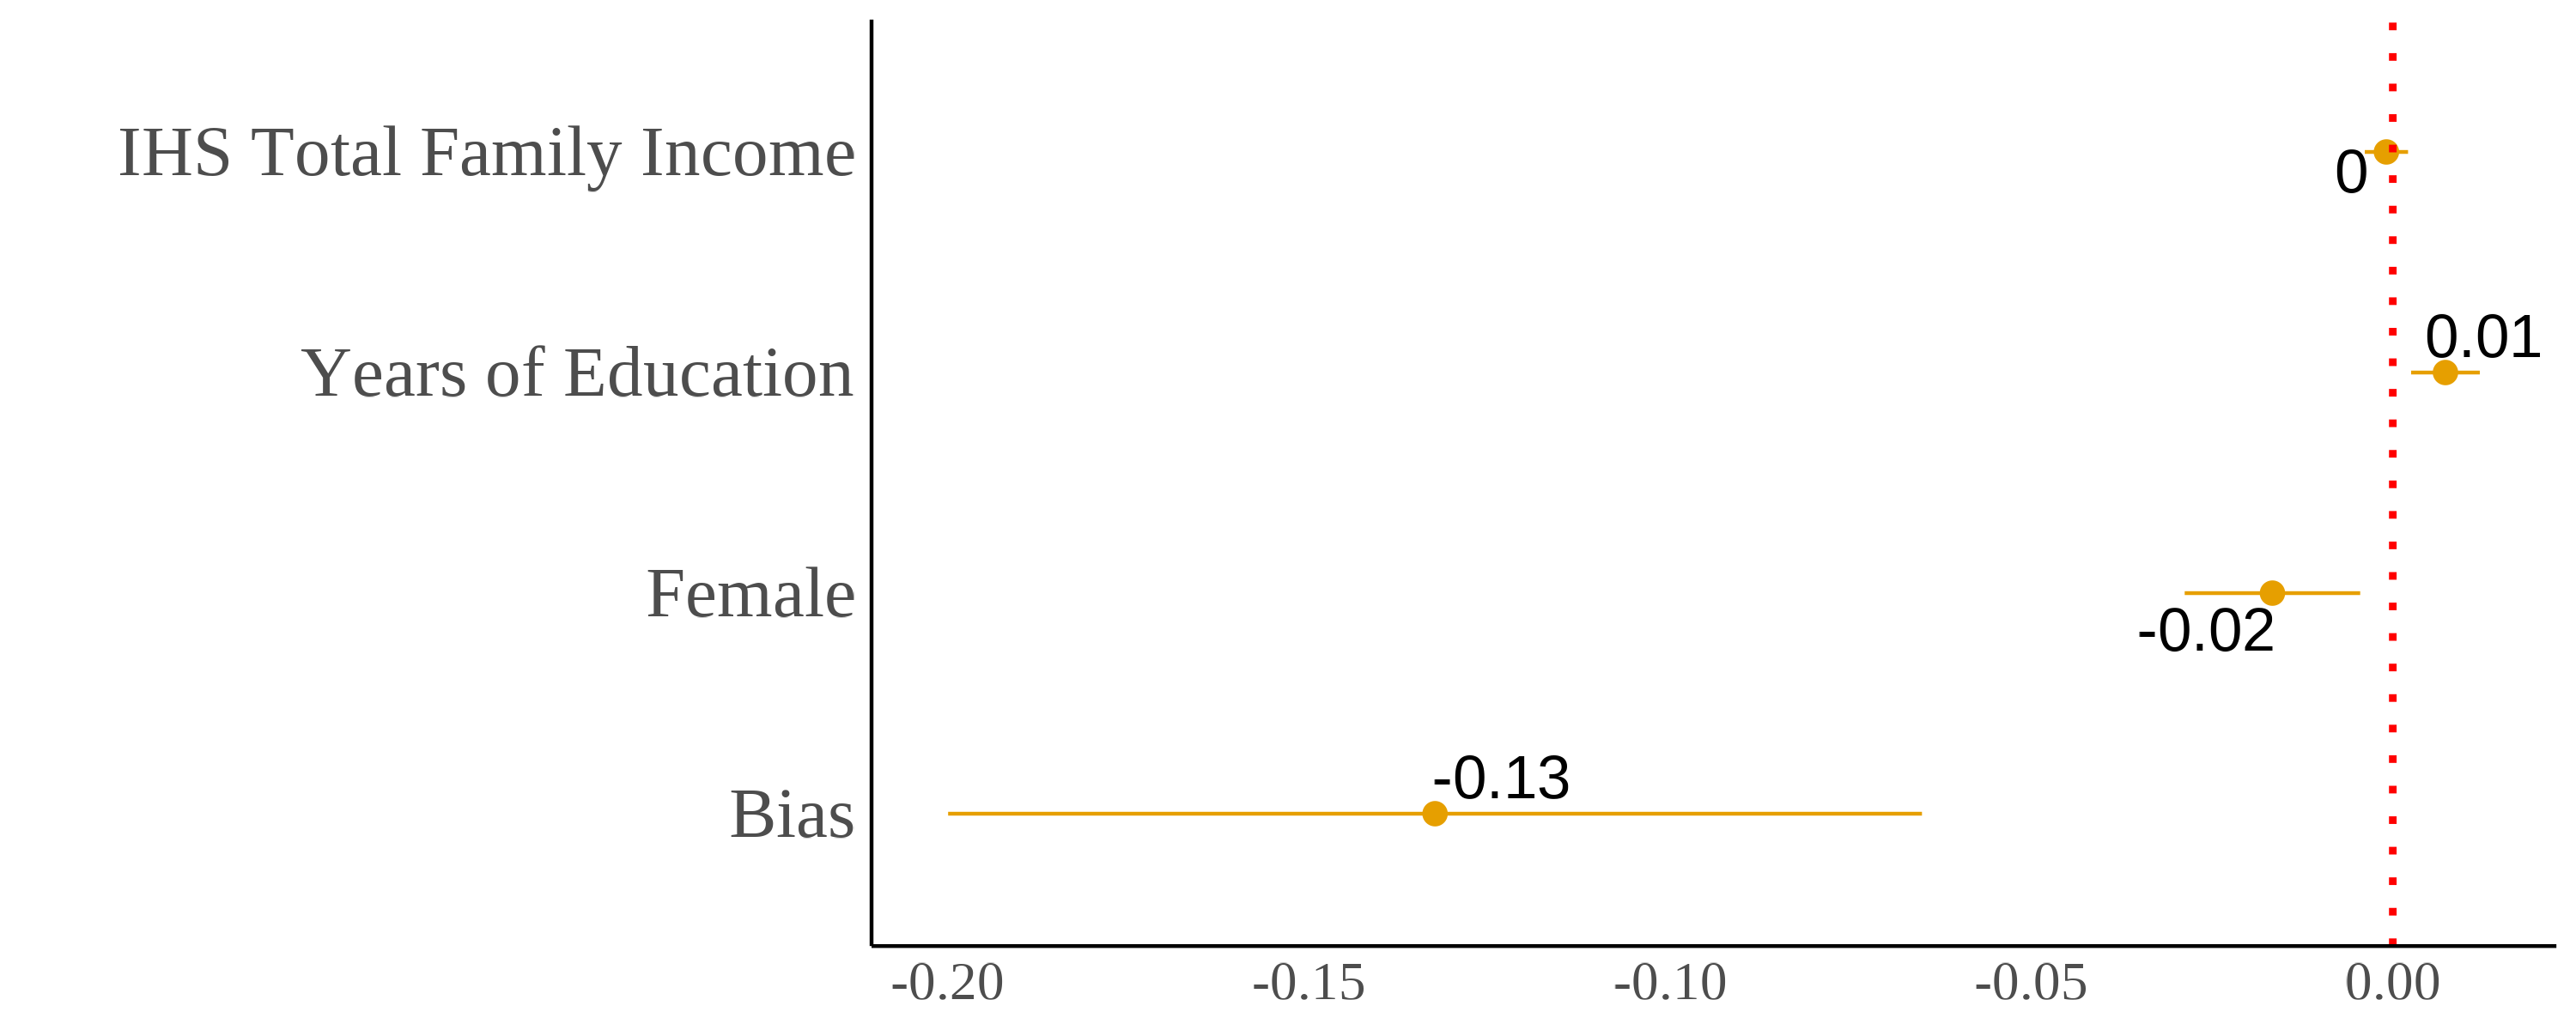
\includegraphics[width=.9\linewidth]{by-parents-regs-all-adults.png}
\end{subfigure}
\centering
%Second graph
\begin{subfigure}{.48\textwidth}
\caption{Asian Fathers-Asian Mothers}
\centering
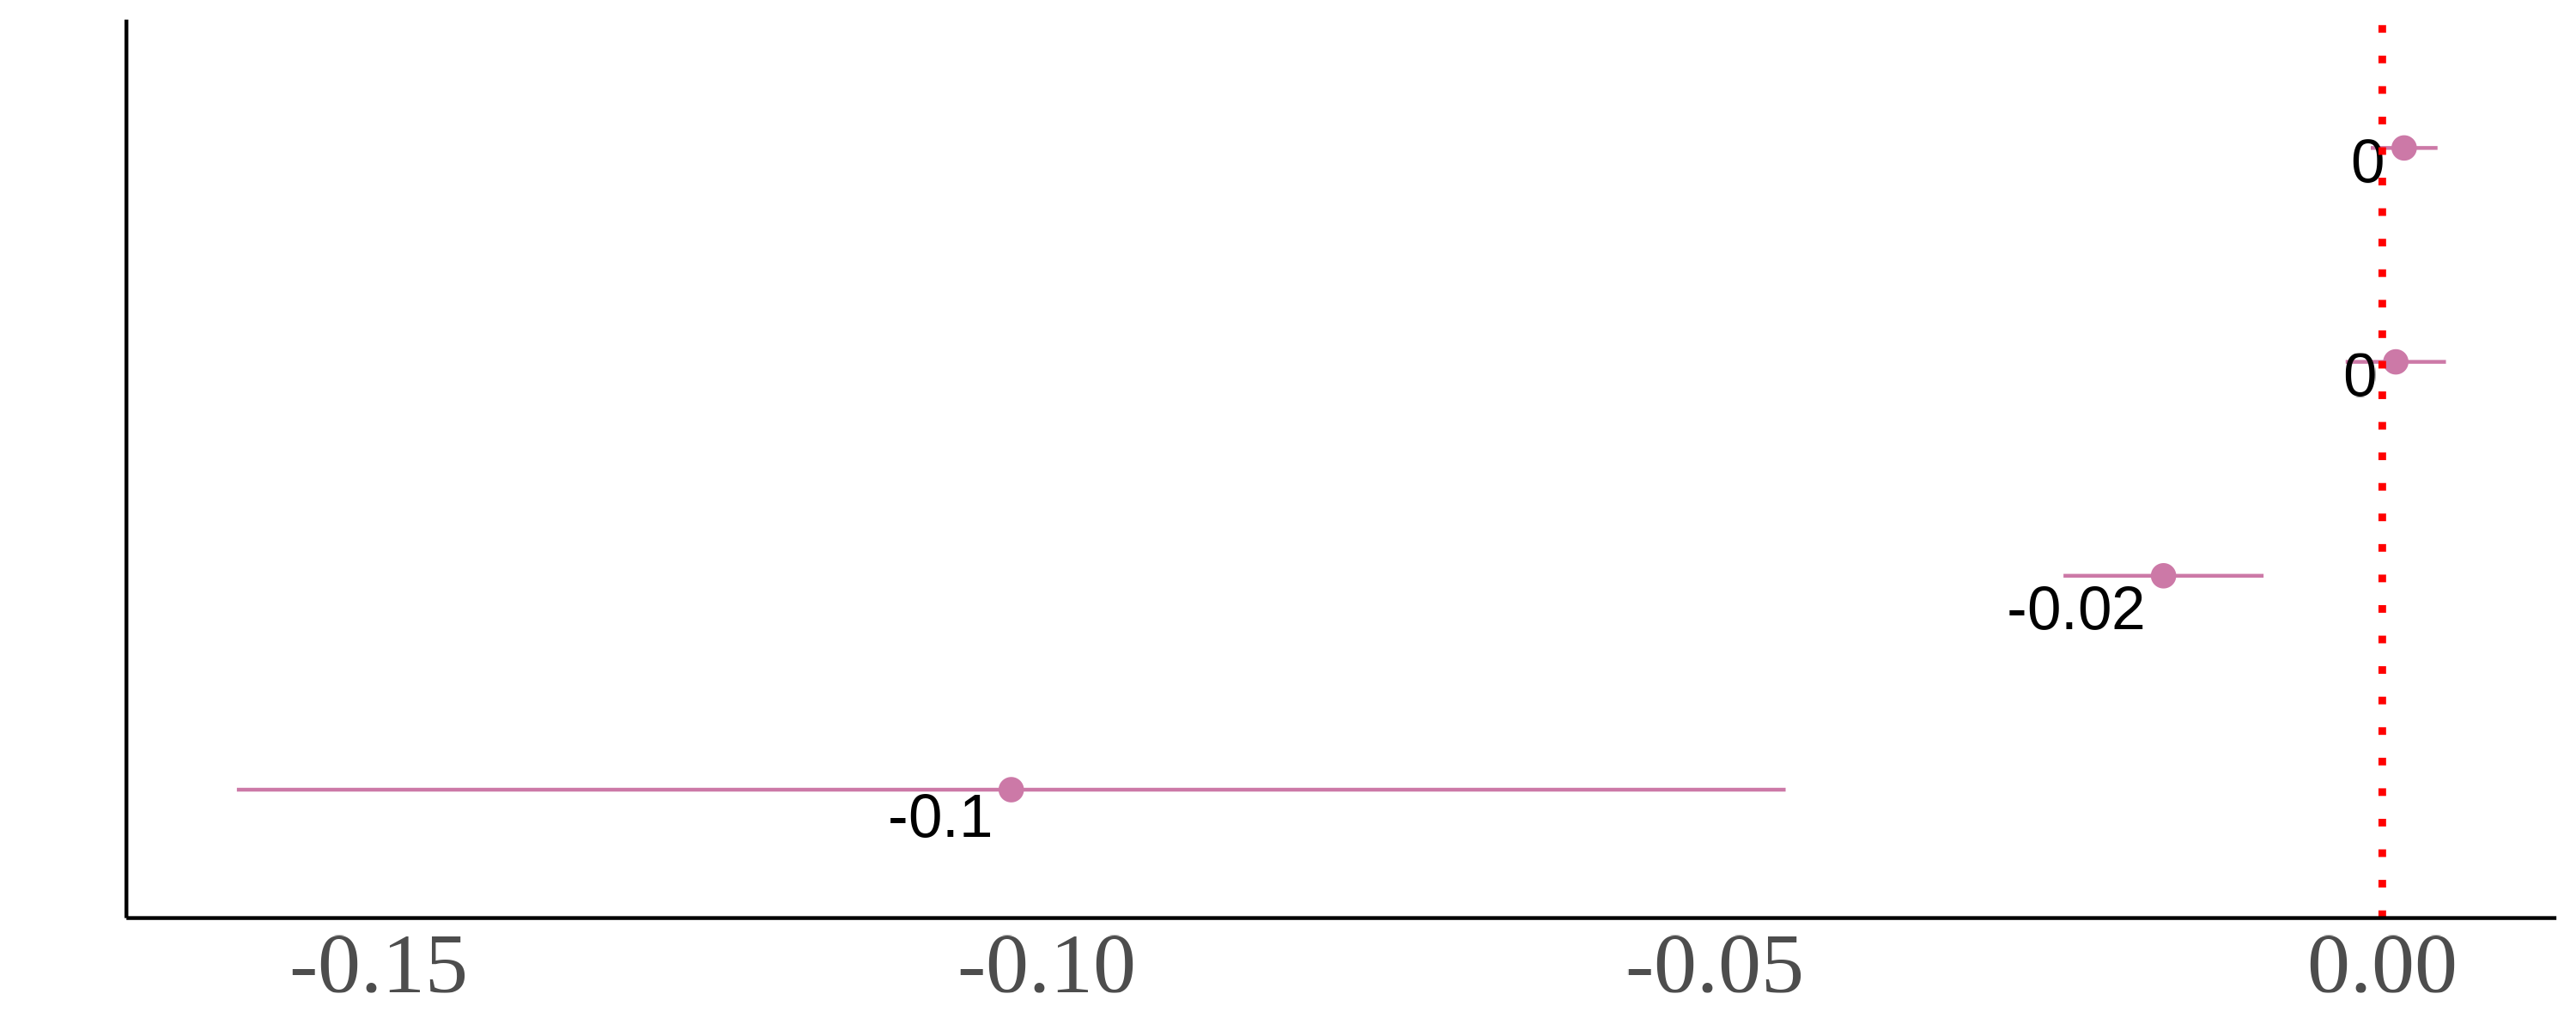
\includegraphics[width=.9\linewidth]{by-parents-regs-hh-adults.png}
\end{subfigure}
%Third Graph
\begin{subfigure}{.48\textwidth}
\caption{Asian Fathers-White Mothers}
\centering
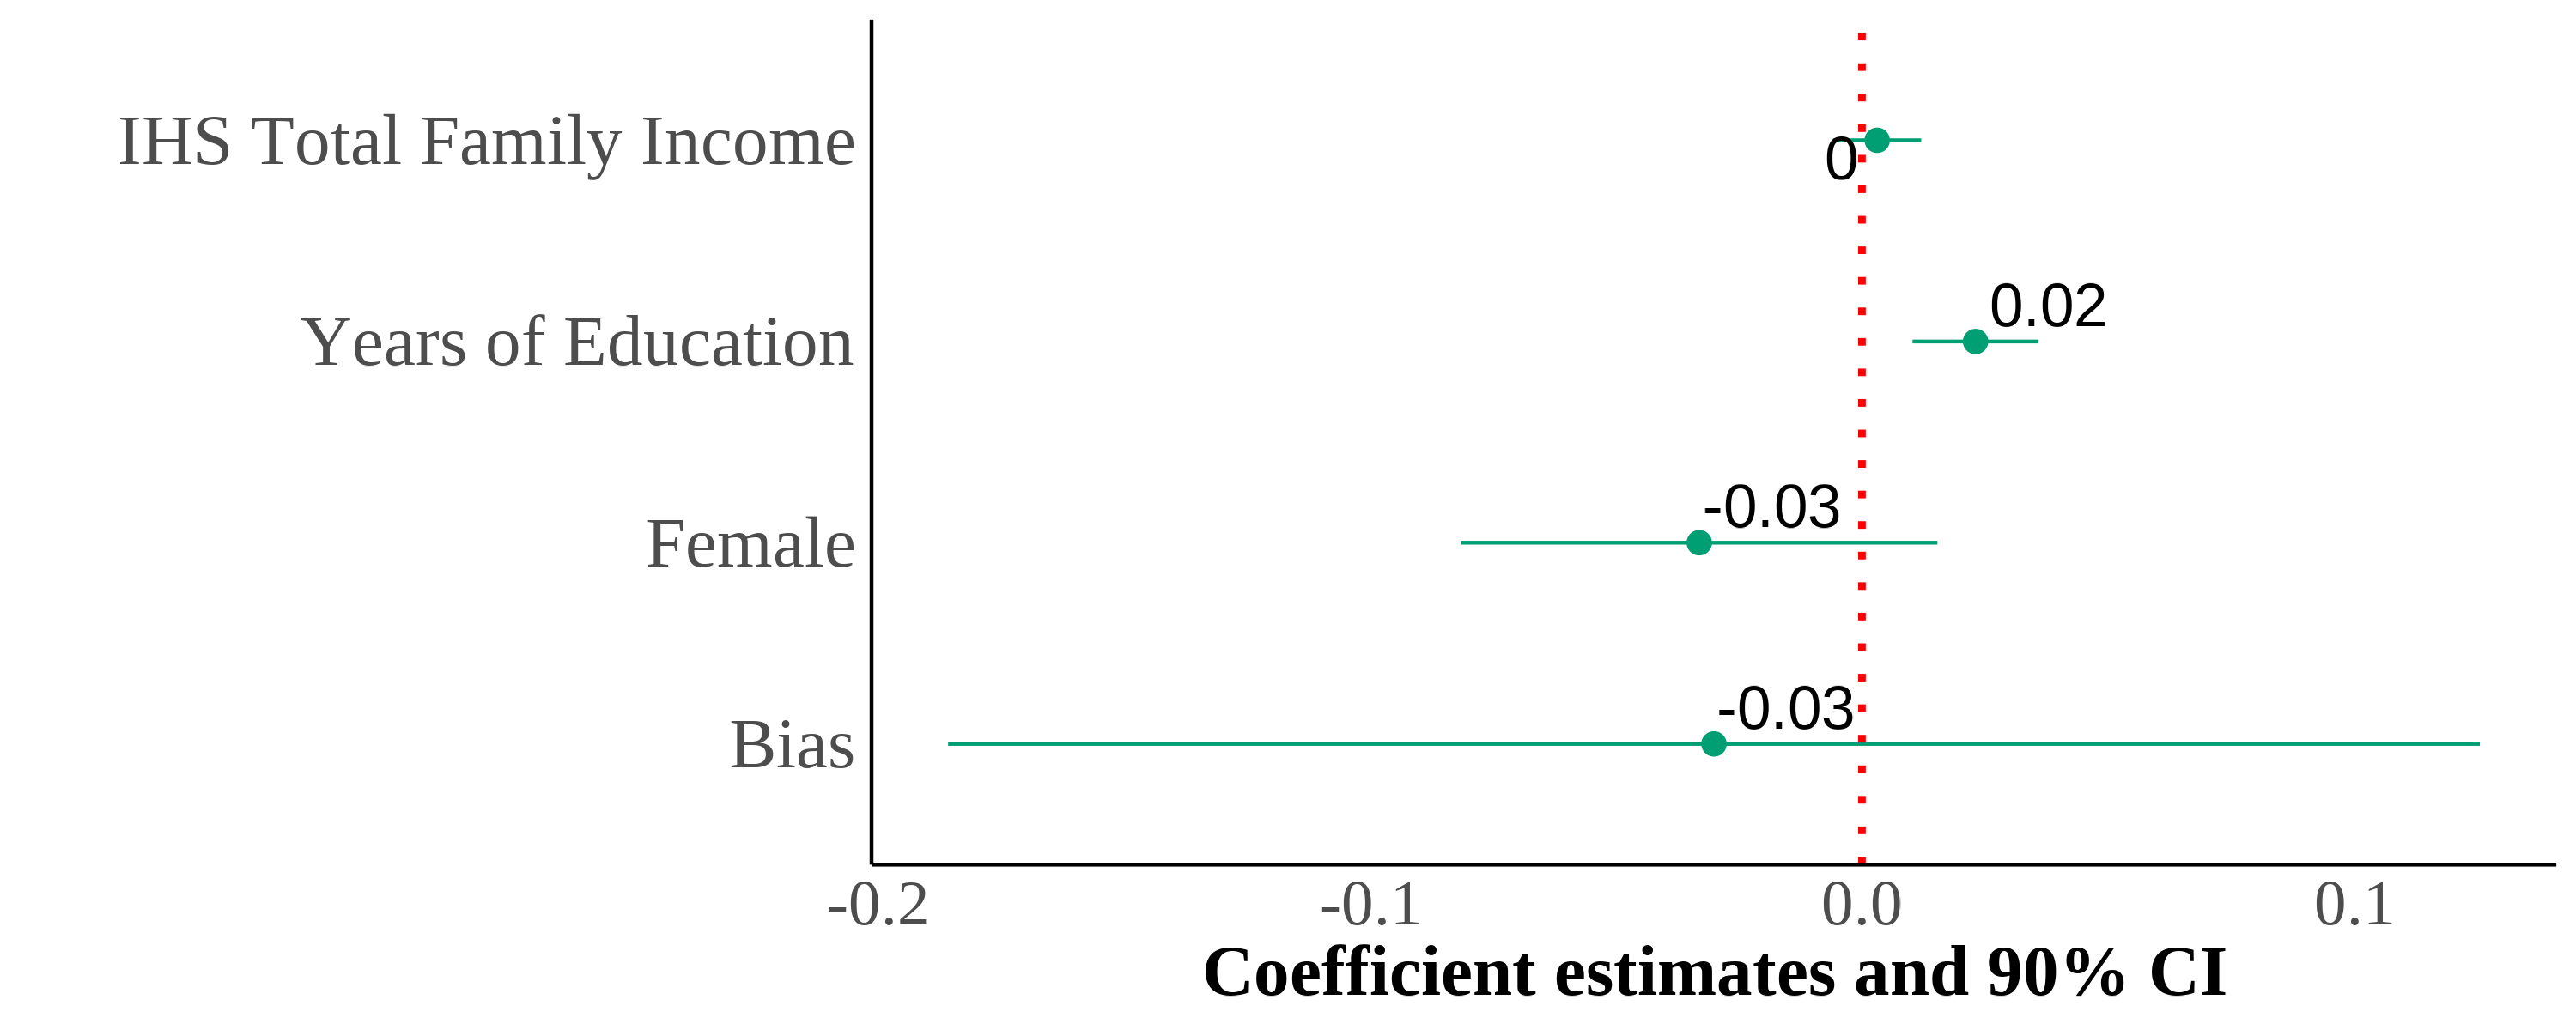
\includegraphics[width=.9\linewidth]{by-parents-regs-hw-adults.png}
\end{subfigure}
%Fourth Graph
\begin{subfigure}{.48\textwidth}
\caption{White Fathers-Asian Mothers}
\centering
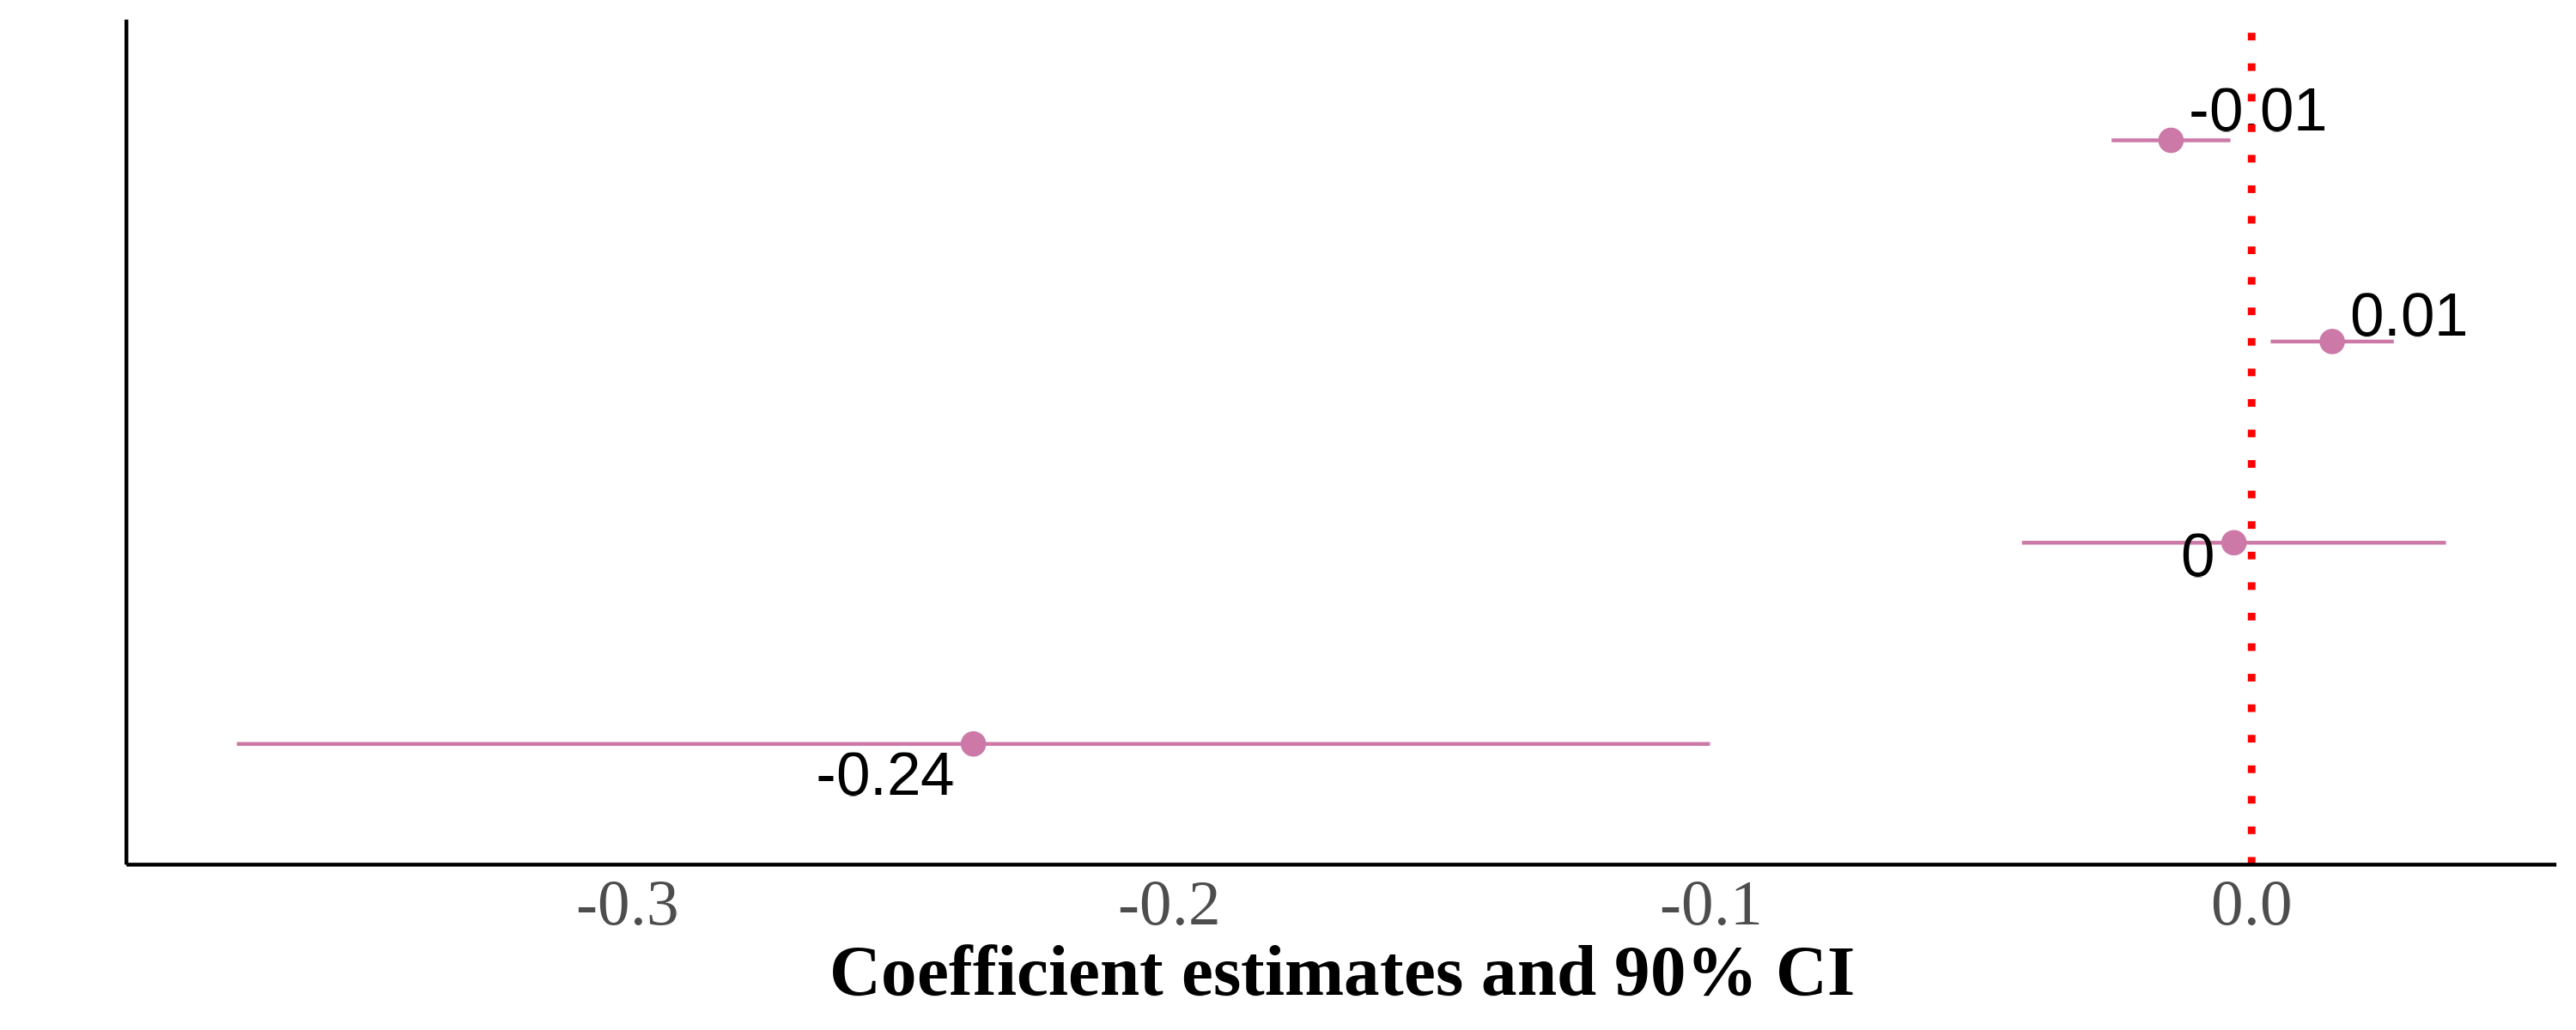
\includegraphics[width=.9\linewidth]{by-parents-regs-wh-adults.png}
\end{subfigure}
\caption*{\footnotesize{I show four panels of estimating equation (\ref{eq:identity_reg_bias}) on a sample of adults. I include region $\times$ year fixed effects with controls for sex, quartic age, years of education, and the inverse hyperbolic sine of income. The dependent variable is self-reported Asian identity and the independent variable is state-level bias. Each panel results from the same regression but on different samples divided by parental types. Standard errors are clustered on the state level. The samples include second-generation Asian individuals ages 18 and above. Native-born second-generation Asian immigrant individuals with at least one parent born in an Asian country.}}
\end{figure}
\end{center}


\pagebreak
\newpage

\begin{table}[H]

\caption{Relationship Between Bias and Self-Reported Hispanic identity Among Third-Generation Hispanic Immigrants: By Grandparental Type \label{regtab-bygrandparents}}
\centering
\resizebox{\linewidth}{!}{
\begin{threeparttable}
\begin{tabular}[t]{lcccc}
\toprule
\multicolumn{1}{c}{ } & \multicolumn{4}{c}{Number of Hispanic Grandparents} \\
\cmidrule(l{3pt}r{3pt}){2-5}
  & \specialcell{(1) \\ One} & \specialcell{(2) \\ Two} & \specialcell{(3) \\ Three} & \specialcell{(4) \\ Four}\\
\midrule
Bias & -0.04 & 0.03 & 0.19 & -0.14*\\
 & (0.11) & (0.09) & (0.26) & (0.07)\\
Female & -0.01 & 0.00 & -0.01 & 0.00\\
 & (0.01) & (0.01) & (0.01) & (0.01)\\
College Graduate: Mother & -0.11*** & -0.07*** & 0.02 & -0.02\\
 & (0.03) & (0.02) & (0.02) & (0.01)\\
College Graduate: Father & -0.11*** & -0.08*** & 0.02 & -0.03*\\
 & (0.03) & (0.01) & (0.01) & (0.01)\\
\midrule
Observations & 55,051 & 74,100 & 12,194 & 57,646\\
Year $\times$ Region FE & X & X & X & X\\
\bottomrule
\multicolumn{5}{l}{\rule{0pt}{1em}* p $<$ 0.1, ** p $<$ 0.05, *** p $<$ 0.01}\\
\end{tabular}
\begin{tablenotes}
\small
\item[1] \footnotesize{Each column is an estimation of equation (\ref{eq:identity_reg_bias}) restricted to third-generation Hispanic immigrants by 
                      number of Hispanic grandparents with region × year fixed effects. 
                      I include controls for sex, quartic age, fraction of Hispanics in a state, and parental education.
                      Standard errors are clustered on the state level.}
\item[2] \footnotesize{The samples include third-generation Hispanic children ages 17 and below who live in intact families. 
                      Native-born third-generation Hispanic 
                      immigrant children with at least one grandparent born in a Spanish-speaking 
                      country.}
\item[3] \footnotesize{Data source is the 2004-2021 Current Population Survey.}
\end{tablenotes}
\end{threeparttable}}
\end{table}


\pagebreak
\newpage

\begin{table}[H]
\centering\centering
\caption{Relationship Between Bias and Interethnic Marriages \label{regtab-logit-02}}
\centering
\begin{threeparttable}
\begin{tabular}[t]{lccc}
\toprule
\multicolumn{2}{c}{ } & \multicolumn{1}{c}{Asian Men} & \multicolumn{1}{c}{Asian Women} \\
\cmidrule(l{3pt}r{3pt}){3-3} \cmidrule(l{3pt}r{3pt}){4-4}
  & \specialcell{(1) \\ Interethnic} & \specialcell{(2) \\ Interethnic} & \specialcell{(3) \\ Interethnic}\\
\midrule
Bias & $0.04$*** & $-0.01$ & $0.03$**\\
 & ($0.01$) & ($0.01$) & ($0.01$)\\
College Graduate: Wife & $0.04$*** & $0.04$*** & $0.05$***\\
 & ($0.00$) & ($0.01$) & \vphantom{1} ($0.00$)\\
College Graduate: Husband & $-0.01$* & $-0.01$ & $-0.02$***\\
 & ($0.00$) & ($0.01$) & ($0.00$)\\
\midrule
Observations & $69,800$ & $52,103$ & $60,214$\\
Year $\times$ Region FE & X & X & X\\
\bottomrule
\multicolumn{4}{l}{\rule{0pt}{1em}* p $<$ 0.1, ** p $<$ 0.05, *** p $<$ 0.01}\\
\end{tabular}
\begin{tablenotes}
\small
\item[1] \footnotesize{This is the result to estimating (\ref{eq:inter-interethnic}) as a
                      linear probability model.}
\item[2] \footnotesize{I include controls for partners' sex, age, education, 
                      and years since immigrating to the United States.
                      Standard errors are clustered on the household level.}
\item[3] \footnotesize{Data source is the 2004-2020 Current Population Survey Data.}
\end{tablenotes}
\end{threeparttable}
\end{table}


\pagebreak
\newpage

\begin{table}[H]
\centering\centering
\caption{Relationship Between Bias and Migration \label{regtab-mig-01}}
\centering
\resizebox{0.7\textwidth}{!}{
\begin{threeparttable}
\begin{tabular}[t]{lccc}
\toprule
  & \specialcell{(1) \\ Migrated from \\ Birth Place} & \specialcell{(2) \\ Migrated from \\ Birth Place} & \specialcell{(3) \\ $Bias_{ist} - Bias_{ilb}$}\\
\midrule
$Bias_{st}$ & 0.13* &  & \\
 & (0.07) &  & \\
$Bias_{lb}$ &  & -0.03 & \\
 &  & (0.17) & \\
Asian &  &  & 0.02\\
 &  &  & (0.04)\\
Female & 0.00 & -0.01 & 0.00\\
 & (0.00) & (0.00) & (0.02)\\
College Graduate: Mother & 0.01*** & 0.00 & -0.01\\
 & (0.00) & (0.01) & (0.03)\\
College Graduate: Father & -0.03*** & -0.03*** & 0.03\\
 & (0.01) & (0.01) & (0.02)\\
\midrule
Observations & 73,563 & 41,641 & 2,075\\
Mean & 0.15 & 0.15 & -0.1\\
Year $\times$ Region FE & X &  & \\
Birthyear $\times$ Birth Region FE &  & X & \\
\bottomrule
\multicolumn{4}{l}{\rule{0pt}{1em}* p $<$ 0.1, ** p $<$ 0.05, *** p $<$ 0.01}\\
\end{tabular}
\begin{tablenotes}
\small
\item[1] \footnotesize{Each column is an estimation of equations (\ref{eq:migration-3}) in column (1), 
                      (\ref{eq:migration-4}) in column (2), and
                      (\ref{eq:migration-5}) in column (3).}
\item[2] \footnotesize{Column (1) is a regression where the left hand side variable is 
                      a dummy variable that is equal to one if a person migrated from the state
                      were born in and the right hand side variable is bias the year of survey.
                      Column (2) is a regression where the left hand side variable is 
                      a dummy variable that is equal to one if a person migrated from the state
                      were born in and the right hand side variable is bias the year of birth in the state of birth.
                      Column (3) is a regression where the left hand side variable is 
                      the difference between state-level bias during the year of the survey in the current state the 
                      respondent is living in, and state-level bias during the year of birth in the state of birth 
                      and the right hand side variable is self-reported Asian identity. This regression captures
                      the selection of those that self-reported Asian identity into states with different levels of bias.
                      I include controls for sex, quartic age, parental education, fraction of Asians in a state, and region × year fixed effects.
                      Standard errors are clustered on the state level.}
\item[3] \footnotesize{The samples include children ages 17 and below who live in intact families. 
                      Native-born second-generation Asian immigrant children with both
                      parents born in a Asian country. The sample in the column (3) regression is further restricted to only those that migrated from their birth state.}
\item[4] \footnotesize{Data source is the 2004-2021 Census Data.}
\end{tablenotes}
\end{threeparttable}}
\end{table}


\pagebreak
\newpage

\begin{table}[H]
\centering\centering
\caption{Main Effect of Proxy on Second-Generation's Asian Self-identification \label{tab:hispbyproxy}}
\centering
\fontsize{12}{14}\selectfont
\begin{tabular}[c]{>{}lllll}
\toprule
Parents Type & All & Asian-Asian & Asian-White & White-Asian\\
\midrule
\textbf{Proxy:} &  &  &  & \\
\hspace{1em}\textbf{Mother} & 0.72 & 0.97 & 0.37 & 0.3\\
\hspace{1em}\textbf{Father} & 0.72 & 0.97 & 0.39 & 0.29\\
\hspace{1em}\textbf{Self} & 0.87 & 0.97 & 0.23 & 0.31\\
\hspace{1em}\textbf{Others} & 0.88 & 0.96 & 0.6 & 0.54\\
\bottomrule
\end{tabular}
\end{table}

\pagebreak
\newpage


% \begin{table}[!h]
\centering\centering
\caption{Relationship Between Bias and Self-Reported Asian Identity: By Proxy Respondent\label{regtab-proxy-01}}
\centering
\resizebox{\ifdim\width>\linewidth\linewidth\else\width\fi}{!}{
\begin{threeparttable}
\begin{tabular}[t]{lcccccc}
\toprule
\multicolumn{1}{c}{ } & \multicolumn{6}{c}{Proxy Respondent} \\
\cmidrule(l{3pt}r{3pt}){2-7}
\multicolumn{1}{c}{ } & \multicolumn{1}{c}{White Mother} & \multicolumn{1}{c}{Asian Mother} & \multicolumn{1}{c}{White Father} & \multicolumn{1}{c}{Asian Father} & \multicolumn{1}{c}{Self} & \multicolumn{1}{c}{Other} \\
\cmidrule(l{3pt}r{3pt}){2-2} \cmidrule(l{3pt}r{3pt}){3-3} \cmidrule(l{3pt}r{3pt}){4-4} \cmidrule(l{3pt}r{3pt}){5-5} \cmidrule(l{3pt}r{3pt}){6-6} \cmidrule(l{3pt}r{3pt}){7-7}
  & \specialcell{(1) \\ $A_{ist}$} & \specialcell{(2) \\ $A_{ist}$} & \specialcell{(3) \\ $A_{ist}$} & \specialcell{(4) \\ $A_{ist}$} & \specialcell{(5) \\ $A_{ist}$} & \specialcell{(6) \\ $A_{ist}$}\\
\midrule
Prejudice Measure & 0.04 & -0.06 & -0.09 & 0.03 & 0.02 & 0.07\\
 & (0.07) & (0.05) & (0.06) & (0.03) & (0.07) & (0.06)\\
Female & -0.02 & 0.01 & -0.01 & 0.00 & -0.07* & 0.00\\
 & (0.02) & (0.01) & (0.02) & (0.01) & (0.04) & (0.01)\\
College Graduate: Mother & 0.01 & -0.04** & -0.02 & 0.00 & -0.05 & -0.07***\\
 & (0.03) & (0.01) & (0.02) & (0.01) & (0.05) & (0.01)\\
College Graduate: Father & 0.00 & 0.00 & 0.02 & 0.01 & -0.02 & -0.02\\
 & (0.03) & (0.02) & (0.02) & (0.01) & (0.06) & (0.01)\\
Second Gen & -0.06 & -0.10*** & 0.17 & -0.18*** & -1.02*** & -0.44***\\
 & (0.04) & (0.04) & (0.18) & (0.05) & (0.05) & (0.05)\\
\midrule
Observations & 4,330 & 28,374 & 8,686 & 28,506 & 738 & 5,823\\
Year $\times$ Region FE & X & X & X & X & X & X\\
\bottomrule
\multicolumn{7}{l}{\rule{0pt}{1em}* p $<$ 0.1, ** p $<$ 0.05, *** p $<$ 0.01}\\
\end{tabular}
\begin{tablenotes}
\small
\item[1] \footnotesize{Each column is an estimation of a heterogeneous effect of regression (\ref{eq:identity_reg_bias}) by 
                      the proxy household respondent with region × year fixed effects. 
                      I include controls for sex, quartic age, fraction of Asians in a state, parental education.
                      Standard errors are clustered on the state level.}
\item[2] \footnotesize{The samples include children ages 17 and below who live in intact families. 
                      First-generation Asian immigrant children that were born in a 
                      Spanish-speaking county. Native-born second-generation Asian 
                      immigrant children with at least one parent born in an Asian 
                      country. Finally, native-born third-generation Asian immigrant children 
                      with native-born parents and at least one grandparent born in a Spanish 
                      speaking country.}
\item[3] \footnotesize{Data source is the 2004-2021 Current Population Survey.}
\end{tablenotes}
\end{threeparttable}}
\end{table}

% \pagebreak
% \newpage

\clearpage


%%%%%%%%%%%%%%%%%%%%%%%%%%%%%%%%%%%%
% PART V. Appendix
%%%%%%%%%%%%%%%%%%%%%%%%%%%%%%%%%%%%
\appendix
\begin{refsection}

% reset page numbers
\pagenumbering{arabic}
\setcounter{page}{1}
\end{refsection}

% %%%%%%%%%%%%%%%%%%%%%%%%%%%%%%%%%%%%
% % PART VI. Responses to Editor and Referees
% %%%%%%%%%%%%%%%%%%%%%%%%%%%%%%%%%%%%
\begin{refsection}
% Reset section numbering
\setcounter{section}{0}
\renewcommand{\thesection}{\Alph{section}}
\renewcommand{\thesubsection}{\Alph{section}.\arabic{subsection}}
\renewcommand{\thesubsubsection}{\Alph{section}.\arabic{subsection}.\arabic{subsubsection}}

        \section{Responses to Editors and Referee} \label{r&r:responses}
        \begin{spacing}{\rrxspc}
            I would like to thank the editors and the anonymous referees for their insightful comments, suggestions, and effort and time in reviewing this paper. I have addressed all the comments and suggestions in the revised manuscript. Below, I provide a summary of the changes made to the manuscript in response to the comments and suggestions.
        \end{spacing}

    \newpage
    
    \section{Responses to Referee One}
        I would like to thank referee one for the insightful comments and suggestions. Below is a detailed response to the comments and suggestions.
    \begin{spacing}{\rrquote}
    \begin{quotation}
    \textbf{R1: } 1. Beginning with the paper's theoretical account of racial bias and its potential impact on racial identity, I appreciate the author's use of formal theory to present a logical and rational model explaining why bias may affect racial identity. However, I feel the author misses an important literature on racial identity and assimilation that focuses on the behavioral aspects of race and racial identity. While they do briefly touch on some of this literature, I suggest that revisions have a greater focus on the behavioral literature on racial identity and assimilation in addition to the formal model. A good work that I could suggest on this topic is Telles and Ortiz's Generations of Exclusion.
    \end{quotation}
    \end{spacing}
    
    \begin{spacing}{\rrxspc}
        \textbf{Response:} I thank the referee for this suggestion. I have added a paragraph in the introduction discussing Telles and Ortiz's Generations of Exclusion and other related works on racial identity and assimilation. Specifically, I add the following paragraph in the introduction: ``While my formal theoretical model provides a logical framework for understanding how bias affects racial identity, the behavioral literature on racial identity and assimilation offers crucial empirical insights that complement this theoretical approach. Research in this tradition emphasizes how racial identity is not merely a cognitive construct but is actively performed, negotiated, and reconstructed through daily interactions and life experiences \autocite{waters1990ethnic}. \textcite{telles2008generations} study of Mexican Americans demonstrates how individuals strategically adapting their racial presentations across different social contexts while maintaining core identity elements across generations. Similarly, behavioral studies have documented how discrimination experiences shape identity salience and group attachment, with individuals developing adaptive strategies that range from ethnic distancing to reactive ethnicity depending on situational factors \autocite{zhou1997segmented}. This behavioral perspective reveals that racial identity operates as both a response to external categorization and an active process of boundary maintenance \autocite{cornell2006ethnicity}. While this literature has primarily relied on qualitative observations and ethnographic methods to document identity flexibility, the present analysis advances this understanding by quantifying these strategic choices through systematic comparison of objective ancestry measures with subjective racial identification across varying environmental contexts.''
    \end{spacing}
    
    \begin{spacing}{\rrxspc}
    \begin{quotation}
        \textbf{R1: } 2. As for the methods, I have a few concerns that I hope the author can address in future drafts. One concern that looms over the paper for me is that the 'objective' measure of Asian background may not be as objective as it seems. For instance, it is unclear that, say, the children or grandchildren of people who were born to non-asian parents in Asia, for example, on an American military base, would be classified as Asian. I don't think this is a huge concern for the analysis, but it needs to at least be addressed.
        \end{quotation}
        \end{spacing}
        
    \begin{spacing}{\rrxspc}
        \textbf{Response:} I appreciate the referee's attention to this issue. It is a point I address in the paper's data section in the following footnote ``I restrict first-generation cases to those whose parents were born in Asian countries to exclude US citizens born abroad to American parents''. Following the comment, I added a few sentences to clarify this point. Specifically, I added the following sentences in the data section: ``It is important to note that while the ancestry measure provides an objective assessment of Asian heritage, it may not capture all nuances of racial identity. For instance, White individuals with Asian ancestry born to non-Asian parents in Asia, such as on American military bases, may not be classified as Asian in the data. To avoid potential misclassification, I remove individuals who report that they were born abroad of American parents.''
    \end{spacing}    

    \begin{spacing}{\rrxspc}
        \begin{quotation}
            \textbf{R1: } 3. Second, I am concerned that using the state as the unit of analysis for regional bias may be problematic. Perhaps the bias of the community that one grows up in would be better measured at the city or zip-code level. For instance, those who live in Austin, Texas may have a very different experience with bias than those who live in rural west Texas. If the authors could provide even a supplemental analysis in which they analyze this at local level, this would help significantly to alleviate these concerns.
    \end{quotation}
        \end{spacing}
            
    \begin{spacing}{\rrxspc}
            \textbf{Response:} I thank the referee for this suggestion. I agree that using more granular geographic units would provide a more precise measure of local bias. However, there are major data limitations that prevent me from doing so. First, the CPS does not provide geographic identifiers below the county level and only for 45\% of the sample and only for counties with larger populations. Therefore, if used at the county level, I would lose more than half of the sample and potentially introduce bias. Second, even if I had access to more granular geographic identifiers in the CPS, to my knowledge, there are no measures of racial bias at more granular geographic levels. The General Social Survey (GSS), which I use as one of my measures of racial bias, is only representative at the the state level. The American National Election Studies (ANES) is only available at the state level. The Uniform Crime Reports (UCR), which I use to calculate anti-Asian hate crimes, is recommended to not be used at the county level and is not available at lower levels. The Implicit Association Test (IAT) data is the only dataset that available at the county level, however, many social scientists have raised concerns about using the IAT on it's own. Therefore, while I agree with the referee that using more granular geographic units would be ideal, I am limited by data availability. I will add a paragraph to the conclusion discussing this limitation and suggesting that future research could explore this question using more granular geographic units if data becomes available. Specifically, I will add the following paragraph to the conclusion: ``More granular geographic units, such as counties, city, or zip-code level, could provide a more precise measure of local bias. However, data limitations prevent the use of these finer geographic levels in the current analysis. Future research could explore this question using more detailed geographic identifiers if such data becomes available, allowing for a deeper understanding of how local contexts shape racial identity.''

            To strengthen how I address this concern, I have conducted supplemental analyses using county-level and MSA-level Implicit Association Test (IAT) data, which are available at more granular geographic levels than the state-level measures used in the main analysis. These results are presented in Appendix Figures \ref{plot01-regression-gen-county}, \ref{plot01-regression-byparent-county}, \ref{plot01-regression-gen-msa}, and \ref{plot01-regression-byparent-msa}. The patterns observed at the county and MSA levels are consistent with the main state-level findings, showing similar negative relationships between anti-Asian bias and Asian identity reporting across generations and parental types. While these analyses are limited to IAT measures alone (due to data availability constraints for other bias measures at sub-state levels), they provide additional evidence that the documented relationships hold at more localized geographic scales. I have also added a footnote in the main results section directing readers to these supplemental analyses. The footnote reads: ``I show the results using county-level and MSA-level anti-Asian bias measures from the Implicit Association Test (IAT) show similar patterns. I present the county-level results in Figures \ref{plot01-regression-gen-county} and \ref{plot01-regression-byparent-county}, while I show the MSA-level in Figures \ref{plot01-regression-gen-msa} and \ref{plot01-regression-byparent-msa}.''
    \end{spacing}
    
    \begin{spacing}{\rrxspc}
        \begin{quotation}
            \textbf{R1: } 4. Additionally, while I understand why children are of particular interest, I would also like to see what the results look like for Asian adults. Is this phenomenon of calculating one's identity concentrated among children? Do they come to identify more with their Asian roots as they reach adolescence and adulthood? Are the same calculations being made by adults? These are important questions that including the sample of adults could be useful to help answer.
        \end{quotation}
    \end{spacing}

    \begin{spacing}{\rrxspc}
        \textbf{Response:} Thank you so much for this important suggestion. I agree that examining the relationship between bias and racial identity among adults would provide valuable insights into how these dynamics evolve over the life course. To address this comment, I have conducted supplemental analyses using the same empirical strategy on an adult sample (ages 18 and above) from the CPS. I show the summary statistics for the adult sample in Table (\ref{tab:sumstat-adults}) and the ethnic attrition for first- and second-generation Asian adults in Table (\ref{tab:hispbygen-adults}). Moreover, I present the relationship between anti-Asian bias and self-reported Asian identity among adults in Figures \ref{plot01-regression-gen-adults} and \ref{plot01-regression-byparent-adults}. The results indicate that the negative relationship between anti-Asian bias and Asian identity reporting among adults mirrors the patterns observed in children, suggesting that similar identity calculations are at play across age groups.

        I also added the following two discussion of the results in the main text. First: ``I report the results using adult samples in Figure (\ref{plot01-regression-gen-adults}). I present results estimating the main specification for all adults in panel (A) and for first- and second-generation subsamples in panels (B) and (C), respectively. Anti-Asian bias and Asian racial identity reporting exhibit negative associations. One standard deviation anti-Asian bias increases correlate with 5 percentage point decreases in Asian racial identity reporting. Among first-generation Asian American adults, one standard deviation anti-Asian bias increases associate with 2 percentage point decreases in Asian racial identity reporting but is statistically insignificant. Among second-generation Asian American adults, one standard deviation anti-Asian bias increases associate with 13 percentage point decreases in Asian racial identity reporting. '' Second: ``I report the results using adult samples in Figure (\ref{plot01-regression-byparent-adults}). I present results estimating the main specification for all second-generation adults in panel (A) and for AA, AW, and WA children subsamples in panels (B), (C), and (D), respectively. One standard deviation anti-Asian bias increases associate with 13 percentage point decreases in Asian racial identity reporting among second-generation adults. Among second-generation adults with endogamous parents, one standard deviation anti-Asian bias increases associate with 10 percentage point decreases in Asian racial identity reporting but are statistically insignificant. However, one standard deviation anti-Asian bias increases associate with a statistically insignificant 3 percentage point decreases in Asian racial identity reporting among Asian father-White mother adults, and 24 percentage point decreases among White father-Asian mother adults.''
    \end{spacing}

    \begin{spacing}{\rrxspc}
        \begin{quotation}
            \textbf{R1: } 5. Lastly and importantly, it is also unclear to me why the author uses measures of animus towards African Americans from the ANES in their bias index, especially when measures of animus towards Asian Americans are available on the very same study. Here I think the author either needs to make a case for the bias they are interested in being more broad than just bias toward Asian-Americans or they need to reestimate their measures of bias.
        \end{quotation}
    \end{spacing}

    \begin{spacing}{\rrxspc}
       \textbf{Response:} Thank you for this important methodological observation. You raise a valid point about the conceptual alignment between my bias measures and outcomes. Let me clarify my approach: The ANES racial animus questions do primarily focus on attitudes toward Black Americans, I also use measures of animus toward Asian Americans. Research consistently shows that racial prejudices are highly correlated across different minority groups—individuals who express bias toward one racial minority typically hold similar attitudes toward others \autocite{almasalkhi2023links, mora2020antiblackness}. These measures therefore capture general patterns of racial animus rather than group-specific bias alone. Crucially, my composite bias index combines three distinct components: (1) Asian-focused IAT measures, (2) ANES racial animus questions, and (3) hate crimes specifically targeting Asian Americans. This multi-proxy approach effectively weights the overall bias measure toward Asian-specific prejudice (two of three components directly measure anti-Asian sentiment) while incorporating information about the broader racial climate through the ANES measures. This methodological choice serves two purposes: it reduces measurement error through the composite approach while capturing both specific anti-Asian bias and the general environment of racial prejudice that affects all minority groups. I added the following to the text of the manuscript to address the important point the referee raised: ``While the ANES racial animus questions primarily focus on attitudes toward Black Americans, research demonstrates that racial prejudices are highly correlated across different minority groups, with individuals who express bias toward one racial minority typically holding similar attitudes toward others \autocite{almasalkhi2023links, mora2020antiblackness}. These measures therefore capture broader patterns of racial animus that extend beyond anti-Black sentiment specifically. When combined with the Asian-focused IAT measures and hate crimes against Asian Americans in my composite index, this multi-proxy approach weights the bias measure more heavily toward Asian-specific prejudice while still capturing the general racial climate.''
    \end{spacing}
    \clearpage
    \pagebreak

    \section{Responses to Referee Two}
    I would like to thank referee two for the insightful and constructive comments and suggestions. Below is a detailed response to the comments and suggestions.

    \begin{spacing}{\rrquote}
        \begin{quotation}
        \textbf{R2: } 1. The paper reports that roughly 96\% of individuals who were born in Asia or who have two Asian parents report being Asian. Before analyzing this group, it would be essential to understand the 4\% who do not. Do they report being of a single racial group not elsewhere classified (e.g., Indian or Chinese), in which case we might reasonably either exclude them since we do not know what they reported or assume that they chose a subcategory of Asian? Is there any way to determine what proportion might be expats born in Asia (primarily in Hong Kong or Singapore)?
        \end{quotation}
        \end{spacing}
        
        \begin{spacing}{\rrxspc}
            \textbf{Response:}  Thank you for this important question. Allow me to break down your comment into different parts that I would address separately. 

            First, regarding the 4\% of individuals born in Asia or with two Asian parents who do not report being Asian, I have examined their self-reported racial identities. I believe that this comment is related to your other comment below regarding showing the distribution of racial identities among those with Asian ancestry. I will respond to that comment below in more detail. However, to briefly address this point, I added a new section to the manuscript (From the Data: Asian Racial Identity and Attrition) where I show the racial attrition and racial choices among those with Asian ancestry. Specifically, I show which of the following categories they report: (1) Asian only, (2) White only, (3) Asian and White/Pacific Islander, (4) other non-Asian multiracial combinations, (5) Asian combined with other races, and (6) Asian/Pacific Islander. 

            Moreover, my analysis defines Asian countries as East Asian and Southeast Asian nations (China, Hong Kong, Taiwan, Japan, Korea, Mongolia, Cambodia, Indonesia, Laos, Malaysia, Philippines, Singapore, Thailand, and Vietnam), excluding South Asian and Middle Eastern countries. This classification aligns with standard demographic research on East and Southeast Asian populations and reflects shared experiences within these regions. To make this clearer, I have added a footnote in the data section specifying which countries are included in the definition of Asian countries. The footnote reads: ``For this analysis, Asian countries comprise East Asian and Southeast Asian nations, including China, Hong Kong, Taiwan, Japan, Korea, Mongolia, Cambodia, Indonesia, Laos, Malaysia, Philippines, Singapore, Thailand, and Vietnam, but exclude South Asian and Middle Eastern countries, consistent with standard demographic classifications.''


            Finally, regarding your point on the ability using the data to identify expats born in Asian countries (i.e. US citizens born abroad to US parents). It is a point I address in the paper's data section in the following footnote ``I restrict first-generation cases to those whose parents were born in Asian countries to exclude US citizens born abroad to American parents''. To make sure that this would be clear in the paper, I added a few sentences to clarify this point. Specifically, I added the following sentences in the data section: ``It is important to note that while the ancestry measure provides an objective assessment of Asian heritage, it may not capture all nuances of racial identity. For instance, White individuals with Asian ancestry born to non-Asian parents in Asia, such as on American military bases, may not be classified as Asian in the data. To avoid potential misclassification, I remove individuals who report that they were born abroad of American parents.''

    \end{spacing}

    \begin{spacing}{\rrquote}
        \begin{quotation}
        \textbf{R2: } 2. Leaving aside these issues, it is problematic to use a linear probability model when the probability is near 0 or 1. Given the range of bias shown in some of the figures, a coefficient of -.05 suggests that the predicted probability of reporting to be Asian is likely to exceed 1 for a nontrivial number of observations. At the very least, the author should show that the results are robust to using probit and logit. I am more inclined to the view that trying to explain the small proportion of individuals with two Asian parents who do not self-identify as Asian is not likely to be productive.
        \end{quotation}
        \end{spacing}
        
        \begin{spacing}{\rrxspc}
            \textbf{Response:} I thank the reviewer for this important methodological point. To address concerns about the linear probability model's limitations when probabilities approach boundary values, I have estimated both logit and probit models alongside the LPM specifications for all analyses. As shown in Tables \ref{regtab-all-gen}-\ref{regtab-third-gen}, the marginal effects from logit and probit models are remarkably consistent with the LPM coefficients across all generational groups, providing strong evidence for the robustness of the findings.

            Regarding the specific concern about predicted probabilities exceeding 1: the logit and probit specifications, which are bounded between 0 and 1 by construction, yield nearly identical marginal effects, confirming that boundary issues are not driving the results.

            The reviewer raises an interesting point about the substantive focus on the minority who do not self-identify as Asian despite having Asian ancestry. However, this phenomenon represents a theoretically important pattern that motivates my research design choices. This is precisely why I break down my analysis by generation and family structure—to demonstrate how identity switching costs vary systematically across different groups. As outlined in Akerlof and Kranton (2000), individuals face differential costs when changing identities based on their circumstances and social constraints. Those with more proscribed identity choices, such as individuals with two Asian parents who appear phenotypically Asian, face higher switching costs and react differently to their environment than those with less constrained options, such as mixed-race individuals who possess greater phenotypic ambiguity. My findings support this theoretical prediction: while bias effects are statistically insignificant among second-generation children with two Asian parents, they are substantial and significant among children from interracial families (15 percentage points for Asian father-White mother families and 10 percentage points for White father-Asian mother families). I present results for all subgroups both for transparency and to illustrate this crucial heterogeneity in identity switching costs. The systematic relationship between experienced bias and identity reporting across these different constraint structures provides insights into how discrimination shapes ethnic and racial identification processes, with direct implications for measuring racial gaps and understanding the economic mechanisms underlying assimilation patterns.


        \end{spacing}

    \begin{spacing}{\rrquote}
        \begin{quotation}
        \textbf{R2: } 3. The interesting part of the paper concerns individuals of mixed ancestry, most of whom do not identify as Asian. But, the only Asian/not only Asian dichotomy is problematic. What proportion of the “not only Asian” reports being Asian and something else? In general, we want to know whether explanatory variables shift mixed-race individuals from reporting themselves as Asian only to something else only, or to biracial.
        \end{quotation}
        \end{spacing}
        
        \begin{spacing}{\rrxspc}
            \textbf{Response:} I appreciate the reviewer's insightful comments on the complexities of racial identity. I believe that addressing this point will significantly enhance my paper. First, to address your comment regarding the distribution of racial identities among those with Asian ancestry, I have added a new section to the manuscript (From the Data: Asian Racial Identity and Attrition) where I show the racial attrition and racial choices among those with Asian ancestry. Specifically, I show which of the following categories they report: (1) Asian only, (2) White only, (3) Asian and White/Pacific Islander, (4) other non-Asian multiracial combinations, (5) Asian combined with other races, and (6) Asian/Pacific Islander. I provide this breakdown for all generations and separately for first-, second-, and third-generation individuals in Figures \ref{fig:histogram-all}-\ref{fig:histogram-thirdgen}. Please see Section \ref{sec:attrition} for the full discussion of these results. 

            The data reveal that among those not identifying as ``Asian only,'' there is substantial variation in identity choices. Among second-generation children from interracial families, 29\% of those with Asian fathers and White mothers report ``Asian and White/Pacific Islander'' (biracial), while 27\% report ``White only.'' Similarly, 40\% of those with White fathers and Asian mothers report ``Asian and White/Pacific Islander,'' while 24\% report ``White only.'' This pattern shows that mixed-ancestry individuals do not simply shift from Asian identification to White identification, but frequently adopt multiracial identities.

            The breakdown becomes even more complex among third-generation individuals. Those with fewer Asian grandparents are more likely to report ``White only'' (54\% for those with one Asian grandparent), while those with more Asian ancestry maintain higher rates of multiracial identification. Critically, even among third-generation children with four Asian grandparents, 92\% still report ``Asian only,'' demonstrating that family composition rather than generational status drives identity flexibility.

            These findings directly address the reviewer's question ``What proportion of the “not only Asian” reports being Asian and something else?'' 

            To further explore how explanatory variables influence these identity choices, I added results from estimating the effects of bias, parental education, and sex using a multinomial logistic regression. This approach allows me to model the probabilities of reporting ``Asian only,'' ``White only,'' and ``Asian and White/Pacific Islander'' as separate outcomes.

            I present the results in Figures \ref{fig:pp-all-gen}-\ref{fig:marginal-effects-third-grandparental}, reveal that anti-Asian bias significantly decreases the likelihood of reporting ``Asian only'' while increasing the probabilities of both ``White only'' and ``Asian and White/Pacific Islander'' identifications among mixed-ancestry individuals. For example, among second-generation children from Asian father-White mother families, a one standard deviation increase in anti-Asian bias is associated with a 12 percentage point decrease in the probability of reporting ``Asian only,'' a 20 percentage point increase in ``White only,'' and a 5 percentage points decrease in ``Asian and White/Pacific Islander.'' To discuss these results, I broke down the results into two subsection. The first subsection--- sub-section \ref{sec:results-dichotomous} titles ``Dichotomous Asian Racial Identity Reporting and Anti-Asian Bias''---discusses the dichotomous outcomes. The second subsection---sub-section \ref{sec:multinomial} titled ``Multinomial Logit Results: Racial Identity Choices and Anti-Asian Bias''---focuses on the multinomial outcomes.

    \end{spacing}

    \begin{spacing}{\rrquote}
        \begin{quotation}
        \textbf{R2: } 4. The paper either doesn’t report basic summary statistics about the distribution of bias, or I missed it. The effect of a one-standard-deviation increase in anti-Asian bias on the probability of reporting only Asian appears to be modest.
        \end{quotation}
        \end{spacing}
        
        \begin{spacing}{\rrxspc}
            \textbf{Response:} I appreciate the reviewer's comments regarding the need for clearer presentation of the bias measures. In the original manuscript, I provided several maps and figures illustrating the geographic distribution of anti-Asian bias across states. In Figure \ref{fig:toptwobias}, I show the aggregate bias index for the two most biased (North Dakota and Tennessee) and two least biased states (Hawaii and Vermont) in Panel \ref{fig:skiniat}. In Panel \ref{fig:Asian-twostates}, I show the self-reported Asian identity rates for the two most biased and two least biased states to illustrate the differences. This would provide visual evidence of the variation in bias levels across states. For example, a one standard deviation bias increases equivalent to moving from Washington, DC, or Vermont to North Dakota in 2020. Additionally, in Figure \ref{fig:skiniat-maps}, I present maps showing the variation in anti-Asian bias across states and over time for my bias index. The maps are of state-level bias in 2004 (Panel \ref{fig:skiniat-map-2004}), 2008 (Panel \ref{fig:skiniat-map-2008}), 2012 (Panel \ref{fig:skiniat-map-2008}), and 2016 (Panel \ref{fig:skiniat-map-2010}). Finally, I show the average state-level bias over the entire sample period in Figure \ref{fig:iat-map-all}. A discussion of these figures is provided in subsection \ref{sub:lw-bias} titled ``Measuring Anti-Asian Sentiment'' in the data section \ref{sec:data}.
    \end{spacing}

    \begin{spacing}{\rrquote}
        \begin{quotation}
        \textbf{R2: } 5. It is surprising that the paper does not look more carefully at other potential explanatory factors, such as income. This is particularly important because the paper is motivated by the potential bias in measures of Asian/non-Asian disparities. However, unless reporting Asian identity is directly or indirectly related to the outcomes for which we want to measure disparities, to a first approximation, there is no bias in the disparities estimates. For example, if reporting a non-Asian identity is uncorrelated with income, the estimated income of Asians is unbiased. The problem only arises if highincome Asians are more (or less) likely to report themselves as non-Asian.
        \end{quotation}
        \end{spacing}
        
        \begin{spacing}{\rrxspc}
            \textbf{Response:} I would like to thank the reviewer for this important comment. I agree that examining how racial identity reporting correlates with socioeconomic outcomes like income is crucial for understanding potential biases in measuring disparities. The issue of including income is problematic since family income is only available in the Annual Social and Economic Supplements (ASEC) of the CPS, i.e. the March supplement. Therefore, if I were to include income in my analysis, my sample size would be reduced significantly. Moreover, since I agree that income is an important variable to consider, I included parental education as it is a proxy for socioeconomic status. 

            Furthermore, in my analysis of the adult sample, I included individual independent variables that include income. As shown in the paragraph describing Figure (\ref{plot01-regression-byparent-adults}), the adult specifications reveal that higher household income positively correlates with Asian identity reporting. This finding directly addresses the reviewer's concern about potential bias in disparity estimates: higher-income Asian Americans are indeed more likely to report Asian identity, which would lead to overestimation of Asian outcomes and underestimation of the true Asian-White gaps in surveys that rely on self-reported race.

            These results support the reviewer's intuition that the relationship between identity reporting and socioeconomic outcomes is crucial for understanding measurement bias. The positive correlation between income and Asian identity reporting, combined with the differential effects by parental education, suggests that studies measuring Asian-White disparities may indeed be systematically biased, particularly overestimating the assimilation and socioeconomic success of Asian Americans.
    \end{spacing}

    \begin{spacing}{\rrquote}
        \begin{quotation}
        \textbf{R2: } 6. Similarly, any effect of anti-Asian bias on reporting is only important if it affects Asians differentially based on their incomes (or other variables we examine for disparities). Thus, it is somewhat surprising that anti-Asian bias is not interacted with other variables, although I expect that the data are not up to the task.
        \end{quotation}
        \end{spacing}
        
        \begin{spacing}{\rrxspc}
           \textbf{Response:} I appreciate the reviewer's insightful comment about the importance of examining how anti-Asian bias effects vary by socioeconomic characteristics. I have directly addressed this concern through several approaches. First, I estimated interaction models that examine how demeaned state-level bias effects differ by parental education and gender, as presented in Figures (\ref{fig:interaction-coefs-aw-wa}) and (\ref{fig:interaction-coefs-thirdgen-grandparent}). These results reveal that anti-Asian bias effects indeed vary significantly by parental education, particularly among mixed-race families, where individuals with college-educated parents respond differently to above-average state bias levels in their identity reporting decisions.
           
           Second, in my adult sample analysis that includes individual income as a covariate, I am able to examine how bias effects interact with socioeconomic status more directly. The adult specifications show not only that higher household income positively correlates with Asian identity reporting, but also reveal differential patterns of bias responsiveness across income levels. This analysis demonstrates that the relationship between anti-Asian bias and identity reporting is indeed moderated by socioeconomic factors, directly addressing the reviewer's concern about differential effects by income and other variables relevant for measuring disparities.
           
           These interaction analyses confirm that anti-Asian bias does not affect all Asian Americans uniformly—rather, its effects are concentrated among specific socioeconomic groups, which has important implications for understanding potential biases in disparity estimates.
    \end{spacing}

    \begin{spacing}{\rrquote}
        \begin{quotation}
        \textbf{R2: } 7. The argument that parents and children provide similar reports about the child's race is not compelling. Presumably, most children mimic their parents' views and only develop an independent self-concept late in childhood or in adulthood. That doesn’t make the parent’s report or the child’s report uninteresting; it just affects the interpretation.
        \end{quotation}
        \end{spacing}
        
        \begin{spacing}{\rrxspc}
           \textbf{Response:} I would like to thank the reviewer for their thoughtful critique regarding the interpretation of parental versus child reports of racial identity. The reviewer correctly notes that children often internalize parental views and may not develop independent racial self-concepts until later in development. However, I address these concerns multiple ways that reinforce the robustness of my findings.
           
           First, as part of my robustness checks, I directly examine this issue by analyzing reporting patterns by household respondent type in Table (\ref{tab:hispbyproxy}). The empirical evidence shows remarkably consistent patterns across different reporting arrangements, with main Asian racial identity effects of 72 percentage points whether mothers or fathers serve as proxies, and 87 percentage points when children themselves serve as household respondents. This consistency suggests that the underlying phenomenon I am measuring—the relationship between anti-Asian bias and identity reporting—is robust across different respondent types. Furthermore, I explore ethnic attrition patterns among adults. I find that the attrition among adults are similar to those of children, as shown in Table (\ref{tab:hispbygen-adults}), suggesting that proxy reporting aligns with individuals' self-identification. 
           
           Second, and more importantly, I address this concern directly in my robustness analysis by examining adult samples where individuals unambiguously self-report their racial identity. As demonstrated in Table (\ref{tab:hispbygen-adults}) and Figures (\ref{plot01-regression-gen-adults}-\ref{plot01-regression-byparent-adults}), I find similar patterns of ethnic attrition and bias effects among adults. This replication with self-reporting adults confirms that the relationship between environmental bias and identity choices is not an artifact of proxy reporting or parental influence on children's responses.
                      
           The \textcite{antmanEthnicAttritionAssimilation2020} finding that Hispanic identification patterns don't vary by household respondent provides additional external validation for the robustness of racial identity reporting across different respondent arrangements.
           
           The reviewer's point about the interpretation is particularly valuable because it clarifies that whether parents or children are making these identity choices, the mechanism I identify---strategic responses to environmental bias---remains substantively important. If parents are making strategic identity choices in response to anti-Asian bias (whether for themselves or on behalf of their children), this represents exactly the type of adaptive behavior my theory predicts and has the same implications for measurement bias in demographic data. The reviewer's insight helps clarify the phenomenon of interest (bias-responsive identity reporting) operates at the family level, which I think would strengthen rather than weaken the theoretical importance of these findings.

    \end{spacing}

    \begin{spacing}{\rrquote}
        \begin{quotation}
        \textbf{R2: } 8. My memory, perhaps incorrect, is that Akerlof and Kranton primarily discuss identity in terms of prescribed, not proscribed, behaviors. Of course, the requirement to act in a certain way may also be interpreted as a requirement not to act in some other way, but the former is more in line with the presentation in the original paper.
        \end{quotation}
        \end{spacing}
        
        \begin{spacing}{\rrxspc}
           \textbf{Response:} Thank you for pointing out this important distinction regarding Akerlof and Kranton's (2000) framework on identity. In thier paper, they discuss both prescribed and proscribed behaviors as integral components of identity formation and maintenance. I did correct the terminology in the manuscript to align more closely with your point. Specifically, I revised the language to emphasize ``prescribed behaviors''. 
    \end{spacing}

    \begin{spacing}{\rrquote}
        \begin{quotation}
        \textbf{R2: } 9. On page 23, I find the statement “While my aim is not to establish a causal effect of bias on self-reported Asian identity, I intend to illustrate a correlation between anti-Asian bias and self-reported identity” extremely odd. Presumably, the goal is to show that the level of bias causes some Asians to switch between an Asian and non-Asian identity. If not, why is the paper interesting? The following sentence maintains that the existence of a correlation suggests possible bias in other measures, but as discussed above, this is only important if anti-Asian bias interacts with characteristics we are comparing between Asians and others.
        \end{quotation}
        \end{spacing}
        
        \begin{spacing}{\rrxspc}
           \textbf{Response:} I would like to thank the reviewer for pointing out this important issue regarding the framing of my research objectives. I removed the sentence you highlighted.
    \end{spacing}

    \begin{spacing}{\rrquote}
        \begin{quotation}
        \textbf{R2: } 10. The world would be a better place if economists stopped including the final paragraph of the introduction, which we all skip anyway. The body of the introduction should be a sufficient guide without a paragraph telling us that the conceptual framework is in a section called conceptual framework.
        \end{quotation}
        \end{spacing}
        
        \begin{spacing}{\rrxspc}
           \textbf{Response:} I appreciate this feedback and have removed the final paragraph from the introduction to streamline the presentation.
    \end{spacing}

    \begin{spacing}{\rrquote}
        \begin{quotation}
        \textbf{R2: } 11. There is a potentially interesting paper here, but the current version is quite far from that paper. I expect that the paper should focus almost entirely on “Asians” of mixed ancestry. It should begin by showing how those individuals report their race and not simply use an Asian only/everything else dichotomy. It should then explore more fully what determines the choice among the possible responses, rather than just examining the effect of anti- Asian bias. If possible, it should examine whether anti-Asian bias affects “Asians” with different characteristics (education, income, gender) differently It should then return to motivating discussion of bias in the measure of disparities to give us a sense of how important endogenous identity is for our estimates.
        \end{quotation}
        \end{spacing}
        
        \begin{spacing}{\rrxspc}
        \textbf{Response:} I am deeply grateful to the reviewer for these comprehensive and incisive comments, which have fundamentally strengthened this paper. The reviewer's suggestions have helped me sharpen the empirical focus, and better connect the findings to their broader implications for measuring disparities. I particularly appreciate the opportunity to address these substantive critiques, as they have guided me toward a more compelling and policy-relevant analysis.
        
        I would like to specifically point out that your suggestions have been incorporated throughout the revision in several key ways. First, following your recommendation to focus more intensively on mixed-ancestry individuals, I have expanded the analysis to examine AW and WA families separately, as shown in the new interaction analysis in Figures (\ref{fig:interaction-coefs-aw-wa}) and (\ref{fig:interaction-coefs-thirdgen-grandparent}). These results reveal the heterogeneous effects you anticipated and demonstrate that bias responses vary significantly by family composition and socioeconomic characteristics.
        
        Second, I have addressed your call for examining differential effects by incorporating interaction models that show how anti-Asian bias affects individuals differently based on parental education, gender, and income. The adult sample analysis now includes direct income controls and demonstrates the selection effects you highlighted—that higher-income Asian Americans are more likely to maintain Asian identity, leading to potential overestimation of Asian outcomes in standard surveys.
        
        Third, I have strengthened the connection between identity reporting patterns and measurement bias in disparity estimates, directly addressing your concern about the policy relevance of endogenous identity choices. The findings now clearly demonstrate how selective identity reporting could systematically bias our understanding of Asian American socioeconomic outcomes.
        
        Finally, your suggestion to move beyond the Asian only/everything else dichotomy has informed my discussion of the multinomial results, where I examine the full range of identity choices available to mixed-race individuals. These revisions have transformed the paper from a descriptive analysis of identity patterns into a more theoretically grounded examination of how environmental factors shape strategic identity choices with clear implications for demographic measurement and policy research.
    \end{spacing}

    \end{refsection}

\clearpage
\pagebreak

%%%%%%%%%%%%%%%%%%%%%%%%%%%%%%%%%%%%
% PART VII. Online Appendix
%%%%%%%%%%%%%%%%%%%%%%%%%%%%%%%%%%%%
\begin{refsection}
% Reset section numbering
\setcounter{section}{0}
\renewcommand{\thesection}{\Alph{section}}
\renewcommand{\thesubsection}{\Alph{section}.\arabic{subsection}}
\renewcommand{\thesubsubsection}{\Alph{section}.\arabic{subsection}.\arabic{subsubsection}}

% Title Page for Appendix
% special footnote symbols
\renewcommand*{\thefootnote}{\fnsymbol{footnote}}
\begingroup
\doublespacing
\centering
\Large ONLINE APPENDIX \\[1.5em]
\LARGE \PAPERTITLE \\[0.75em]
\large
\AUTHORHADAH\footnote[1]{\AUTHORHADAHINFO}\\[1.0em]
\endgroup
\clearpage

% Online appendix
%%%%%%%%%%%%%%%%%%%%%%%%%%%%%%%%%%%%
% Appendix A, Solution and Estimation Details
%%%%%%%%%%%%%%%%%%%%%%%%%%%%%%%%%%%%

% Set equation, figure, table indexing
\renewcommand{\thefigure}{A.\arabic{figure}}
\setcounter{figure}{0}
\renewcommand{\thetable}{A.\arabic{table}}
\setcounter{table}{0}
\renewcommand{\theequation}{A.\arabic{equation}}
\setcounter{equation}{0}
\renewcommand{\thefootnote}{A.\arabic{footnote}}
\setcounter{footnote}{0}

\section{Data} % (fold)
\label{sec:data-ap}

\begin{figure}[H]
\centering
\caption{Examples of an Implicit Association Test}
\label{fig:iatexamples}
\begin{subfigure}{.48\textwidth}
\centering
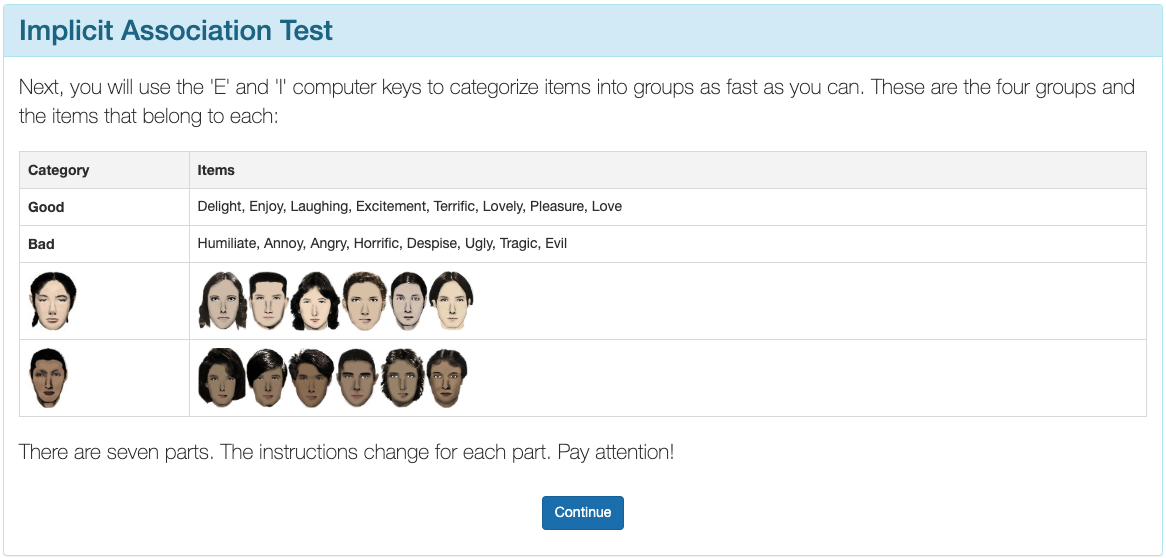
\includegraphics[width=.9\linewidth]{iatexample1.png}
\end{subfigure}
\centering
%Second graph
\begin{subfigure}{.48\textwidth}
\centering
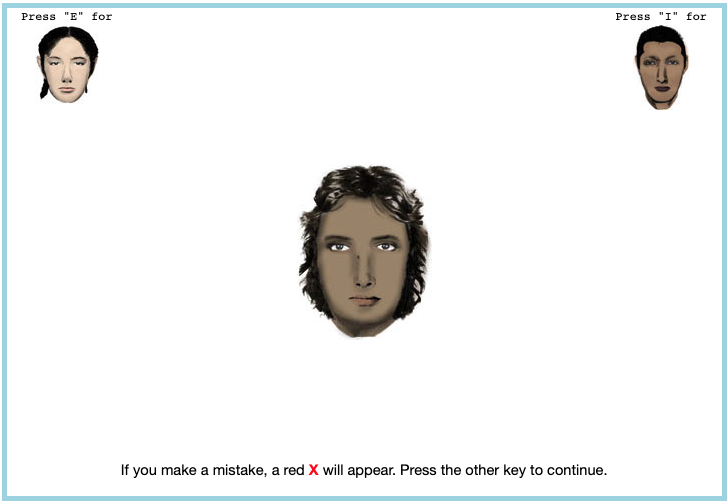
\includegraphics[width=.9\linewidth]{iatexample2.png}
\end{subfigure}
%Third
\begin{subfigure}{.48\textwidth}
\centering
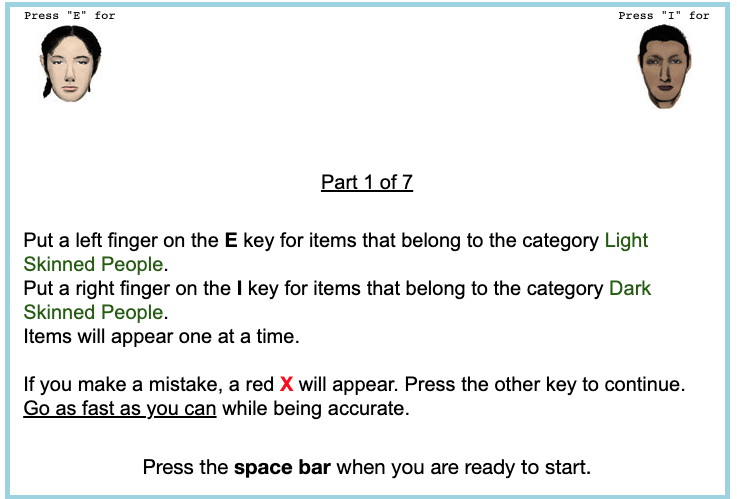
\includegraphics[width=.9\linewidth]{iatexample3.png}
\end{subfigure}
% Fourth
\begin{subfigure}{.48\textwidth}
\centering
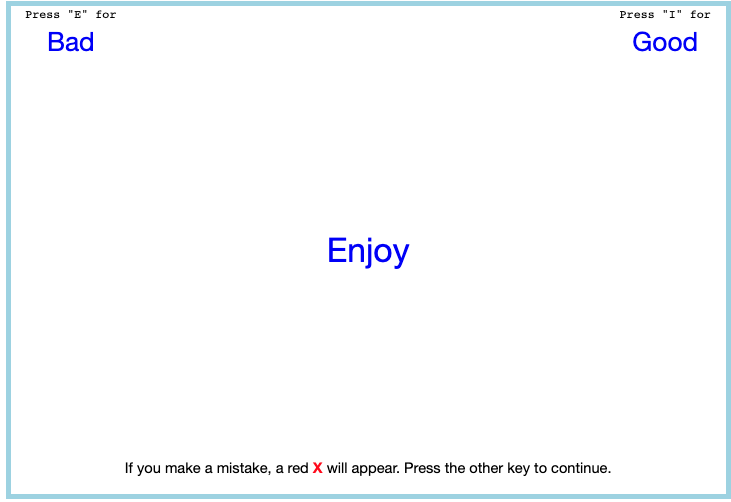
\includegraphics[width=.9\linewidth]{iatexample4.png}
\end{subfigure}
%Fifth
\begin{subfigure}{.48\textwidth}
\centering
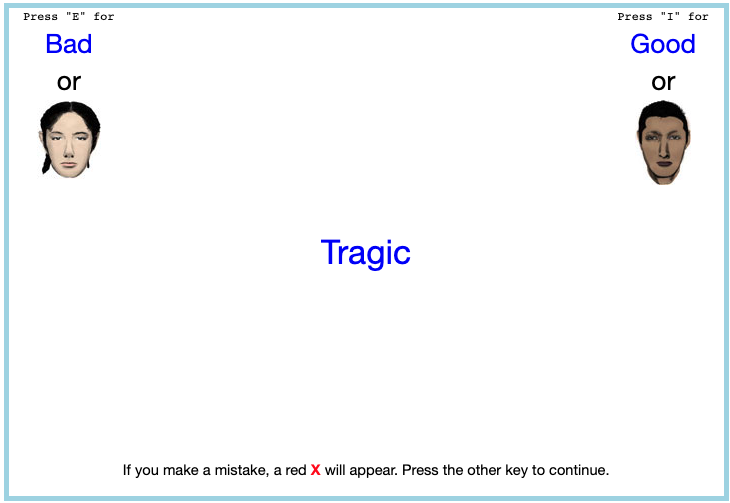
\includegraphics[width=.9\linewidth]{iatexample5.png}
\end{subfigure}
\caption*{\footnotesize{Here are a few examples of what a respondent would see on an implicit association test.}}
\end{figure}

\newpage
\pagebreak

\section{Figures}\label{appendix:figs}

\begin{figure}[H]
    \centering
    \caption{Scatter Plot of Proportion Subjectively Asian on Bias}
    \label{scatter-plot-1}
    \begin{subfigure}{.9\textwidth}
    \caption{Year < 2015}
    \centering
    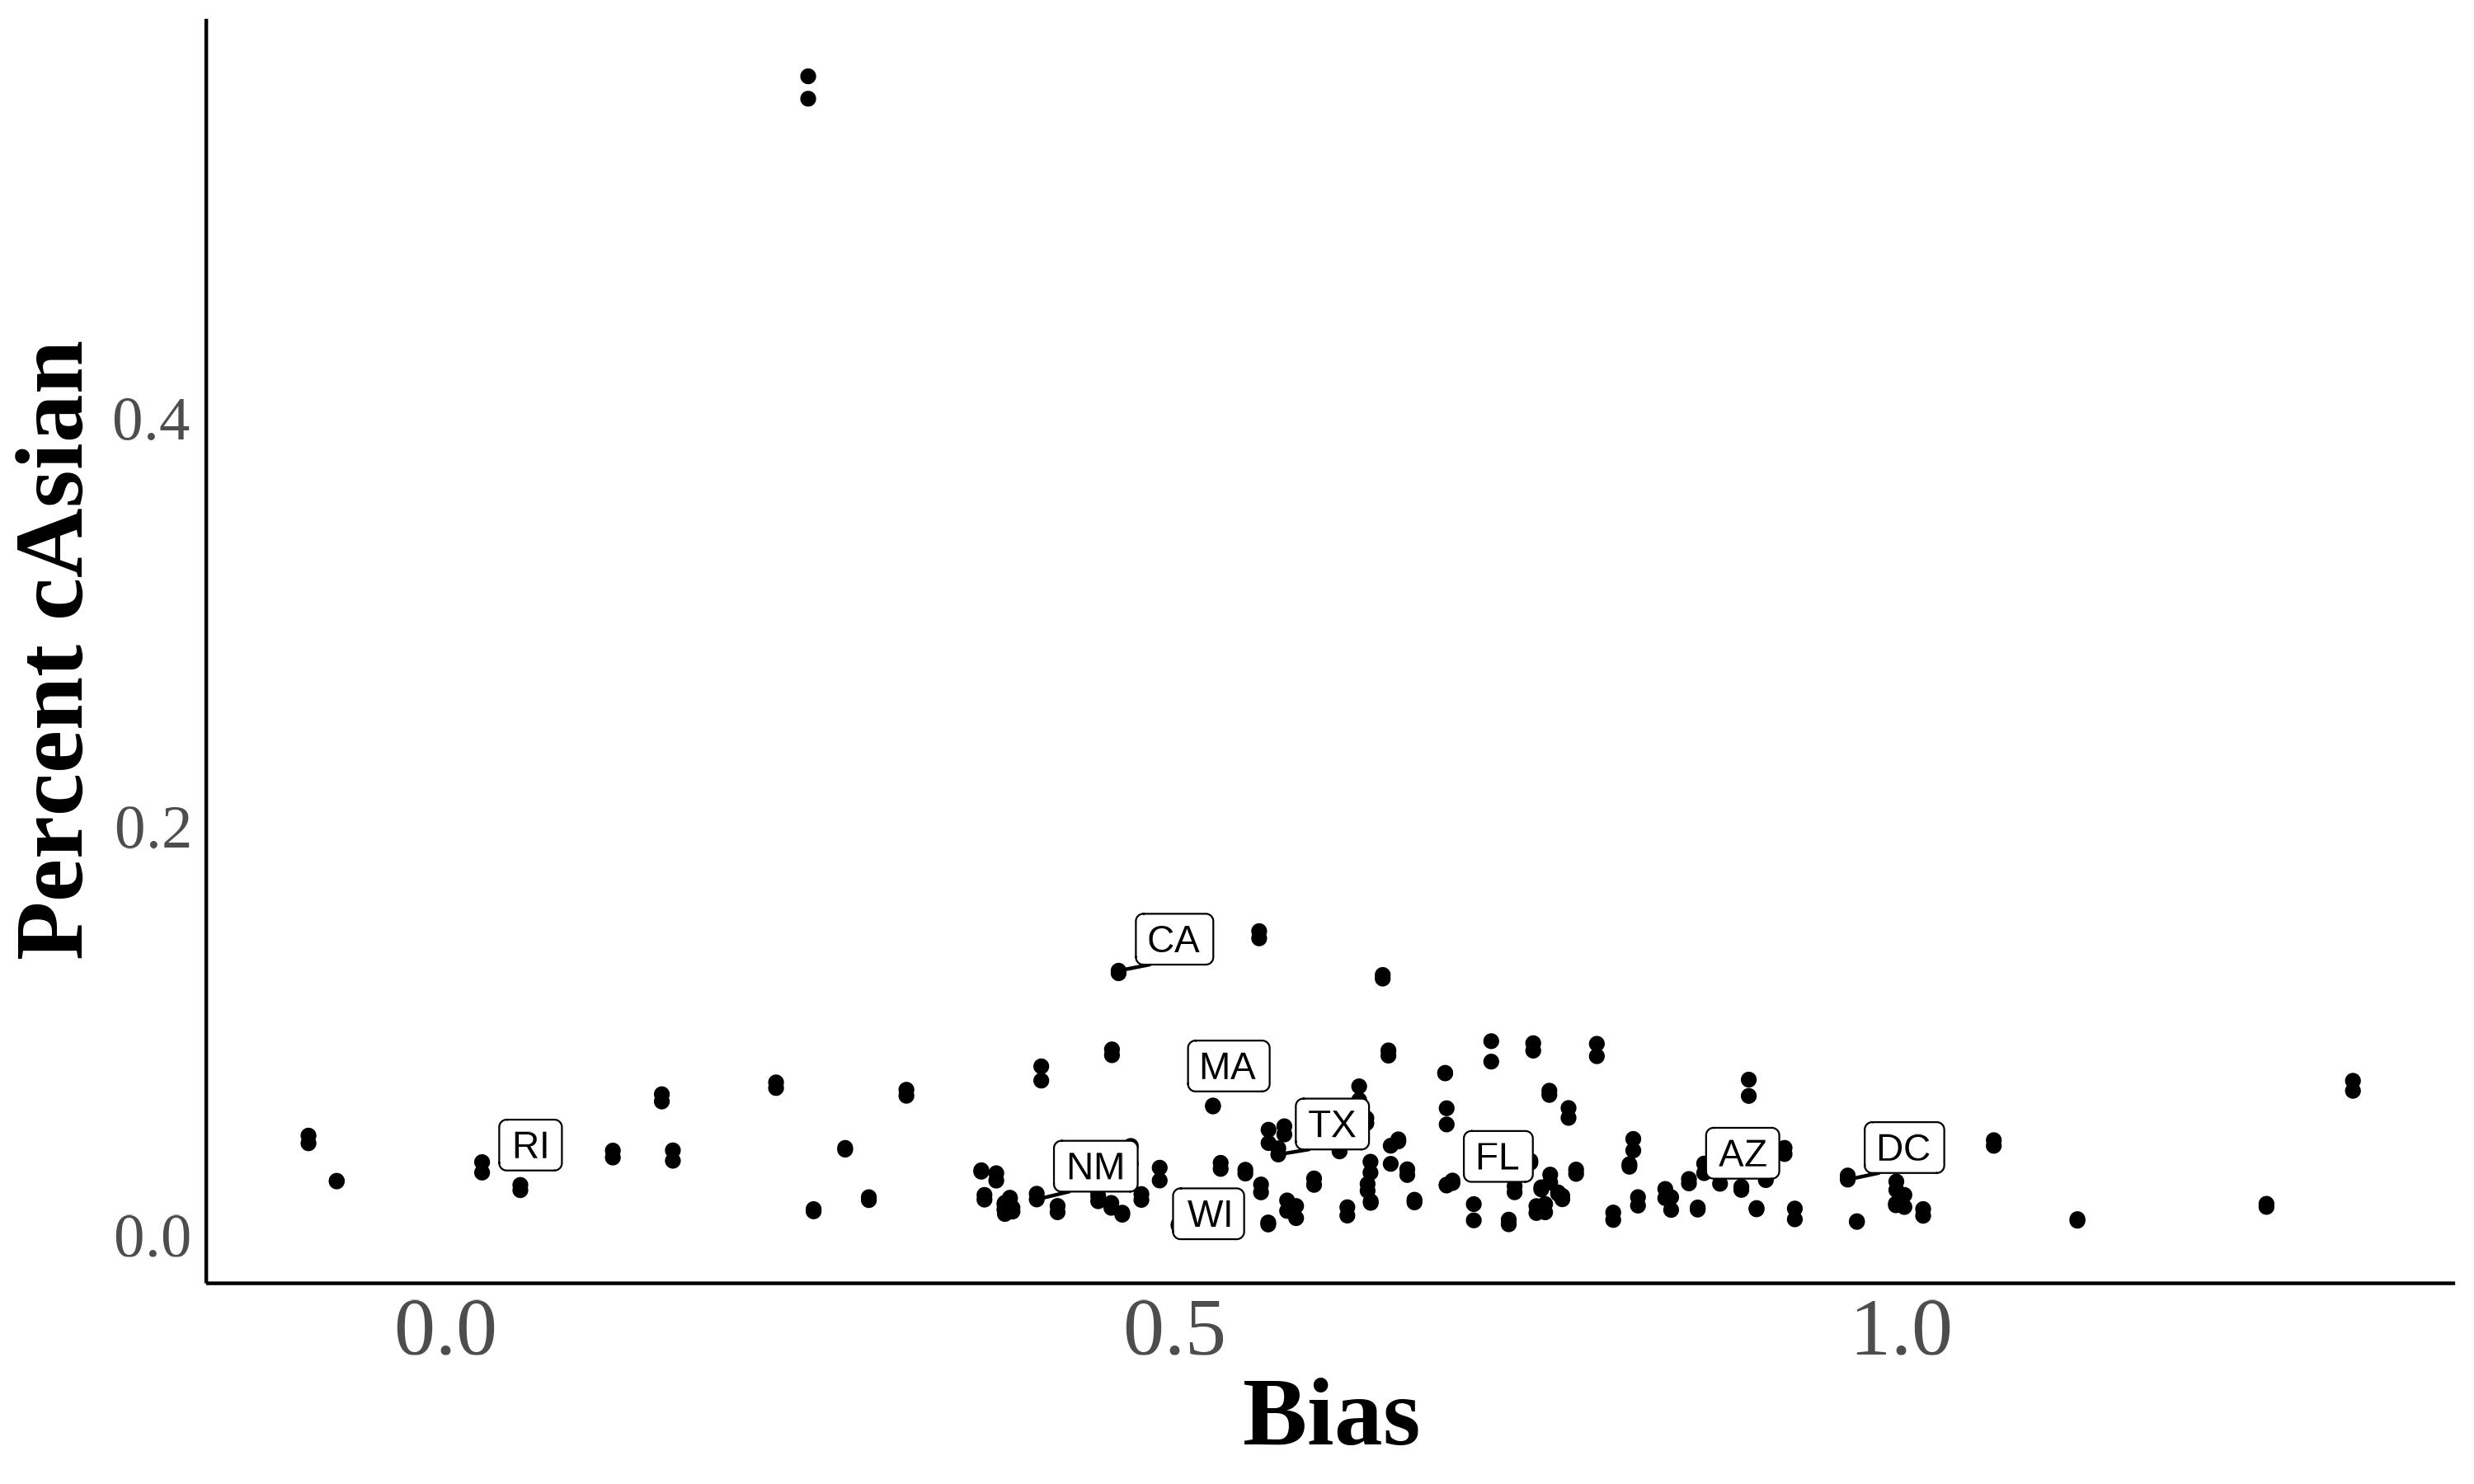
\includegraphics[width=.9\linewidth]{scatter-plot-bias-Asian-less2015.png}
    \end{subfigure}
    \centering
    %Second graph
    \begin{subfigure}{.9\textwidth}
    \caption{Year $\geq$ 2015}
    \centering
    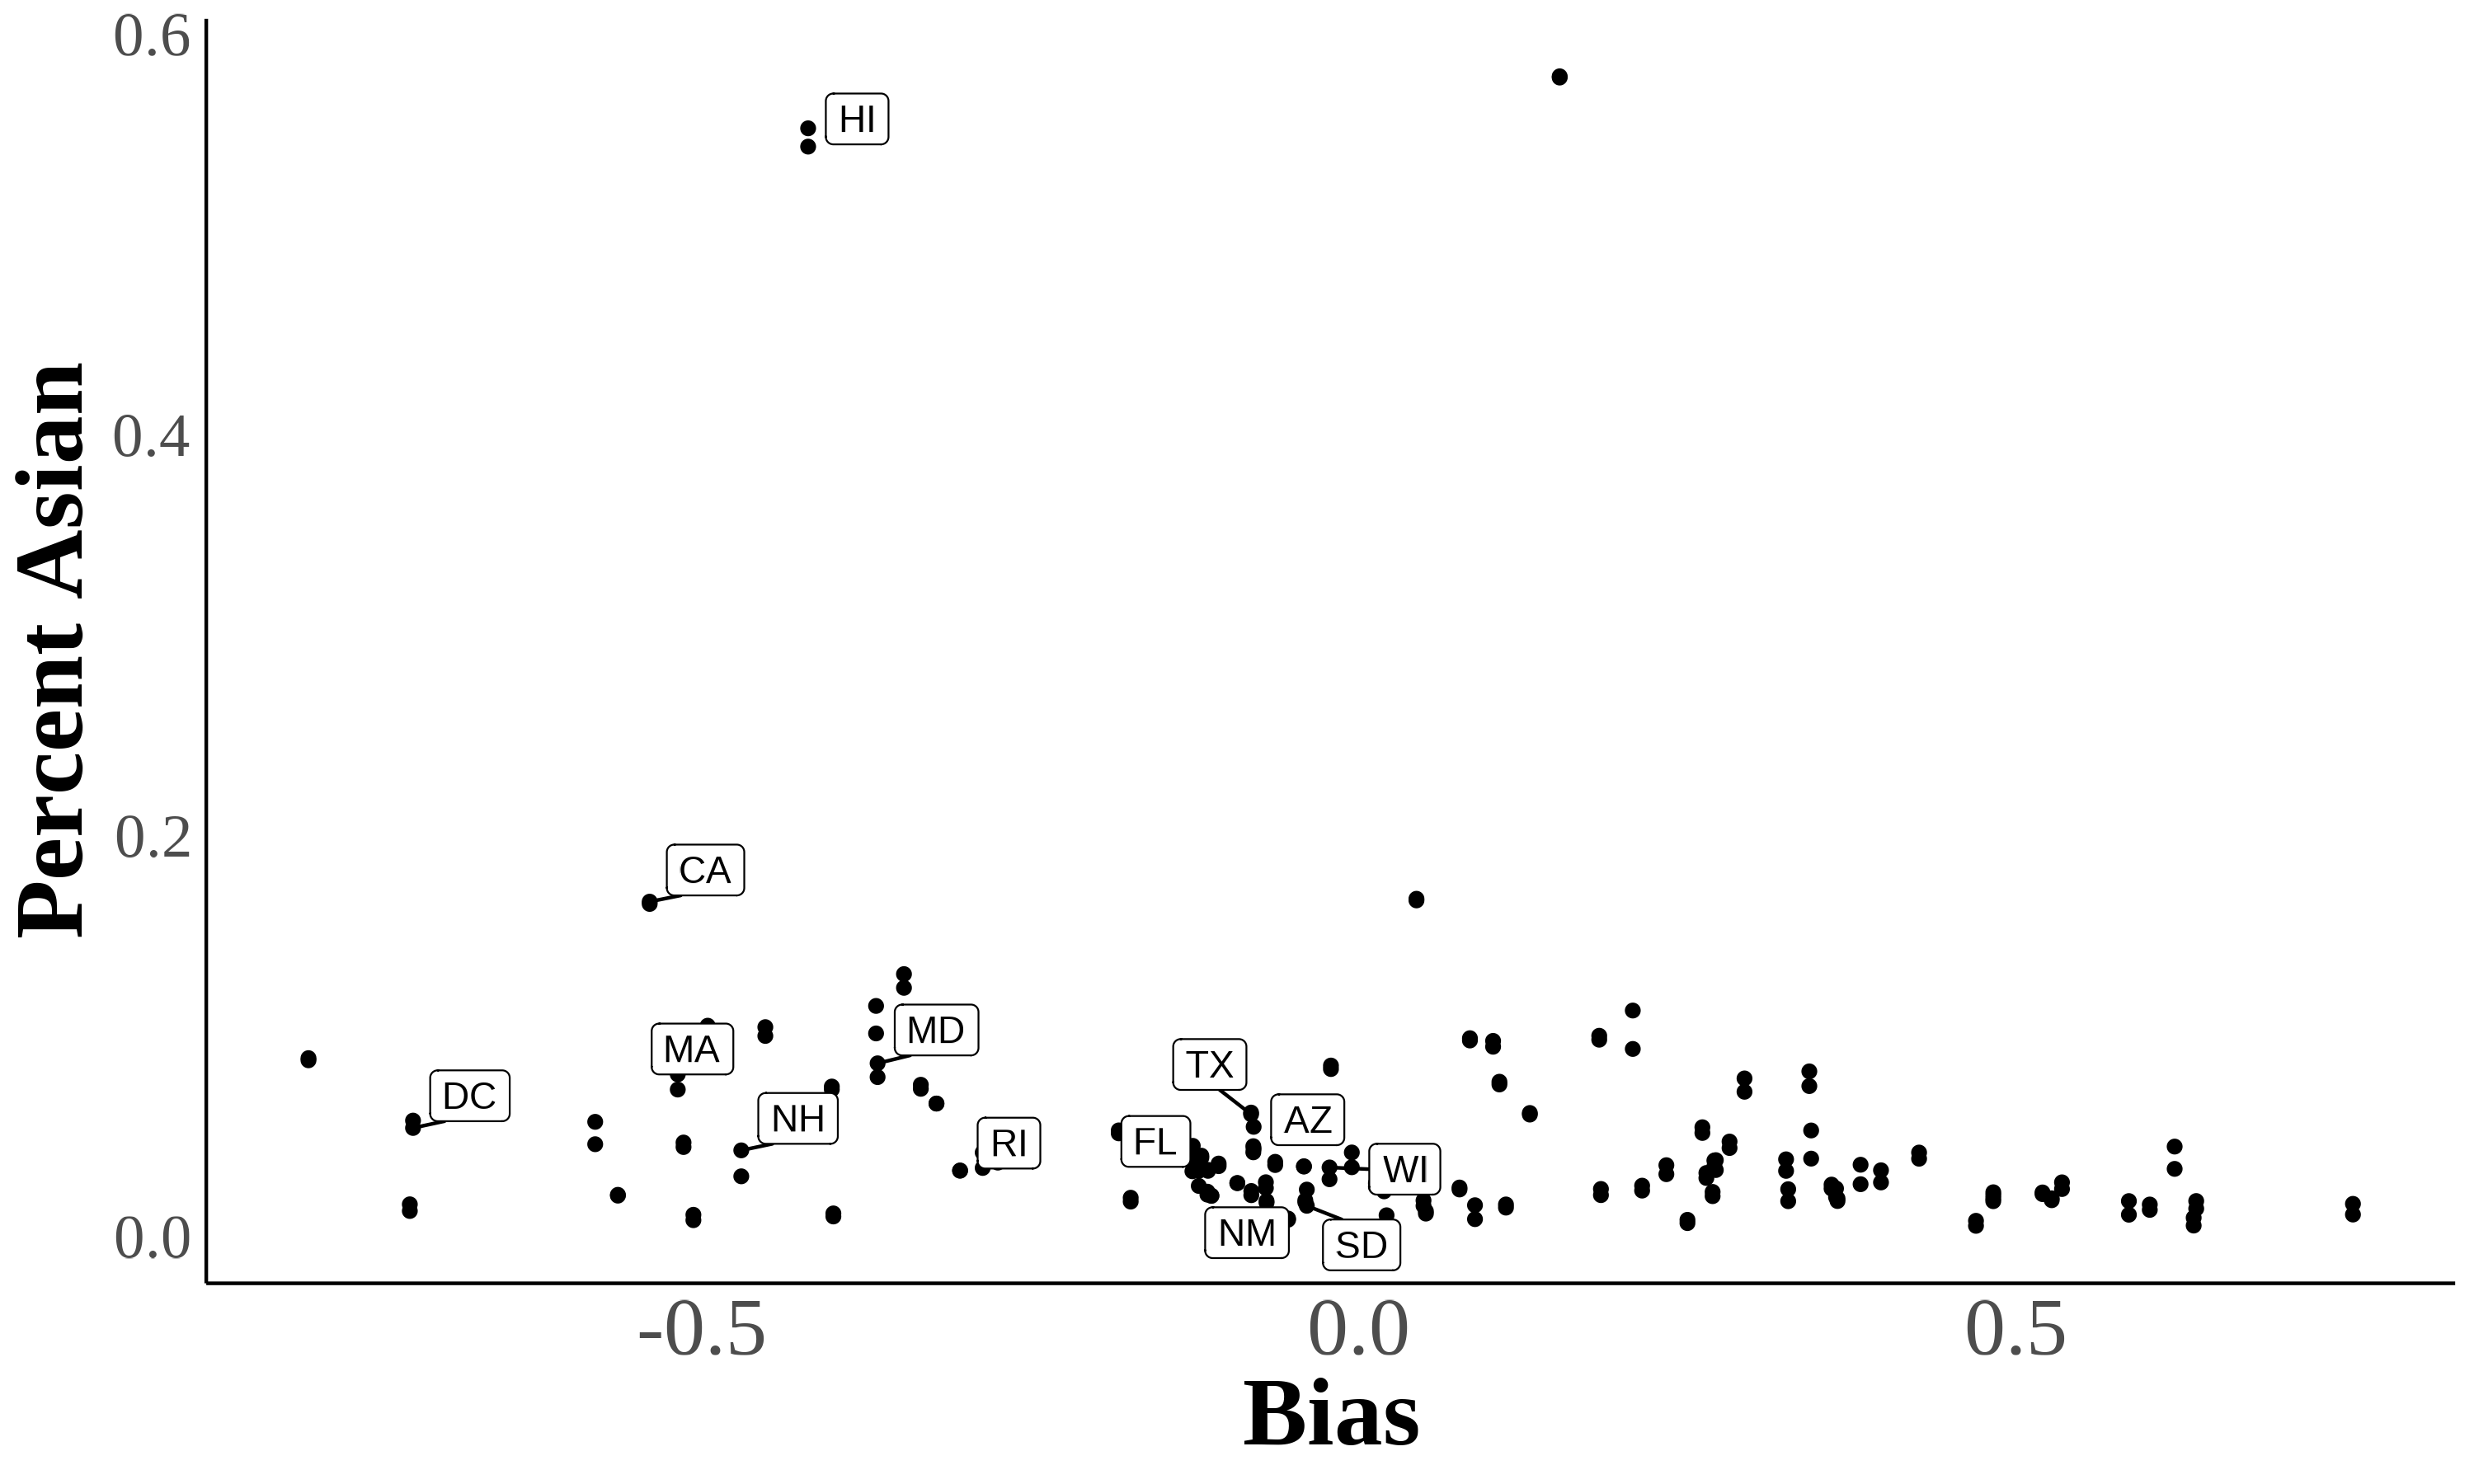
\includegraphics[width=.9\linewidth]{scatter-plot-bias-Asian-great2015.png}
    \end{subfigure}
    \caption*{\footnotesize{Here are two scatter plots showing the relationship between bias and subjective Asian population in a state. Each dot represents a state in a certain year. Percent subjectively Asian = $\frac{\# \text{Asian}}{\text{Population}}$ \\
    \emph{Source.} 2004-2021 Current Population Survey.}}
    \end{figure}
    
\subsection{Using \textcite{lubotskyInterpretationRegressionsMultiple2006} to Construct Bias Index} % (fold)
\label{sub:lw-bias}
In \textcite{lubotskyInterpretationRegressionsMultiple2006}, the authors propose a method to reduce measurement error in proxies by constructing a composite index. The Lubotsky-Wittenberg (henceforth LW) consider a model where a covariate is unobserved. Therefore, they use two proxies in its place, which will have measurement error. Thus, the LW method allows researchers to use two proxies that are error-ridden. 

LW consider a setup with the following model:

\begin{align*}
    y &= \alpha + \beta x^* + \epsilon \\
    x_1 &= x^* + \mu_1 \\
    x_2 &= x^* + \mu_2
\end{align*}

Where \(x_{i}^{*}\) is the unobserved covariate, \(x_{1i}\) and \(x_{2i}\) are the proxies, and the measurement errors \(\mu_1\) and \(\mu_2\) are assumed to be classical and allowed to covary. The covariance matrix of the errors is given by:

\[
\Sigma = \begin{bmatrix}
    \sigma_1^2 & \sigma_{12} \\
    \sigma_{12} & \sigma_2^2
\end{bmatrix}
\]

Replacing the unobserved \(x^*\) with \(x_1\) or \(x_2\) yields the following expectations of the OLS estimates:

\[
\mathbb{E} \left[ \hat{\beta}_1 \right] = \beta \frac{\sigma_{x^*}^2}{\sigma_{x^*}^2 + \sigma_1^2} \quad ; \quad \mathbb{E} \left[ \hat{\beta}_2 \right] = \beta \frac{\sigma_{x^*}^2}{\sigma_{x^*}^2 + \sigma_2^2}
\]

Both estimates are biased; the one with the smaller variance of the measurement error being less biased.

LW then propose defining a new proxy \(x_3\) as a weighted average of \(x_1\) and \(x_2\):

\[
x_3 = \lambda x_1 + (1 - \lambda) x_2
\]

To minimize the attenuation bias in the OLS estimate of \(\beta\), they solve for the optimal value of \(\lambda\):

\[
\lambda^* = \frac{\sigma_2^2 - \sigma_{12}}{\sigma_1^2 + \sigma_2^2 - 2\sigma_{12}}
\]

This optimal value of \(\lambda\) is not directly useful because the variances of the measurement errors and their covariance are unobserved. However, if you estimate a bivariate regression using OLS (i.e., regress \(y\) on \(x_1\) and \(x_2\)), then the expectation of the sum of the two coefficient estimates is identical to the expectation of the OLS coefficient estimate on \(x_3\) in a univariate regression using the optimal choice of \(\lambda\):

\[
\mathbb{E} \left[ \hat{\beta}_1 + \hat{\beta}_2 \right] = \mathbb{E} \left[ \hat{\beta}_{x_3} \right]
\]

Thus, OLS produces an estimate of \(\beta\) with the least bias by optimally combining the information in \(x_1\) and \(x_2\).


\newpage
\pagebreak

% Appendix Bibliography
\begingroup
\setstretch{1.0}
\setlength\bibitemsep{0pt}
\printbibliography[title=References for Online Appendix]
\endgroup
\pagebreak
\end{refsection}

\end{document}